
\guideline[g:nontext:figure_vector_graphics]
    {Figures: Use vector graphics.}

% bad: make bad screenshot of vector graphics
\goodbadexample[{\cite[Fig.~6]{Wetzlinger2023TAC}}]{
    \begin{center}
        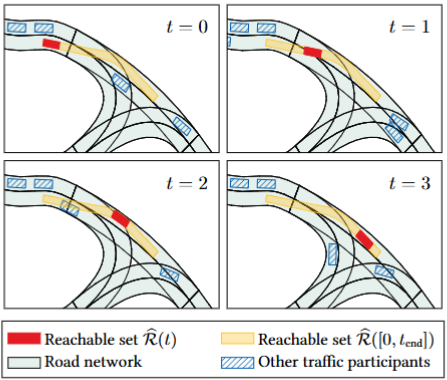
\includegraphics[scale=0.7]{data/figure_vectorgraphics_bad.png}
    \end{center}
}{
    \definecolor{good_blue}{RGB}{0, 92, 171}
\definecolor{good_red}{RGB}{227, 27, 35}
\definecolor{good_gray}{RGB}{230, 241, 238}
\definecolor{good_yellow}{RGB}{255, 195, 37}
%
\begin{center}
\begin{tikzpicture}
\pgfplotsset{
plotstyle1/.style={area legend, draw=black, fill=good_gray, thin, forget plot},
plotstyle2/.style={area legend, draw=black, forget plot},
plotstyle3/.style={area legend, draw=good_blue, pattern = north east lines, pattern color=good_blue, forget plot},
plotstyle4/.style={area legend, draw=good_yellow, fill=good_yellow, fill opacity=0.35, forget plot},
plotstyle5/.style={area legend, draw=good_red, fill=good_red, forget plot}
}
% to put axis lines on top!
\pgfplotsset{
	layers/axis lines on top/.define layer set={
		axis background,
		axis grid,
		axis ticks,
		axis tick labels,
		pre main,
		main,
		axis lines,
		axis descriptions,
		axis foreground,
	}{/pgfplots/layers/standard},
}
\def\rows{2}
\def\cols{2}
\def\horzsep{0.15cm}

\begin{groupplot}[%
group style={rows = \rows, columns = \cols, horizontal sep = \horzsep, vertical sep=\horzsep},
scale only axis,
set layers=axis lines on top,
width=4cm,height=2.75cm,
legend style={legend columns=2,legend to name=legendname, legend cell align=left,/tikz/every even column/.append style={column sep=0.75cm}},
xmin=-730,xmax=-670,ymin=-805,ymax=-770,ticks=none
]
\nextgroupplot[]

\addplot[plotstyle1]
table[row sep=crcr] {%
x	y\\
-746.62	-781.5\\
-748.79	-782.8\\
-752.13	-784.43\\
-754.38	-785.26\\
-756.71	-785.87\\
-759.06	-786.2\\
-761.41	-786.24\\
-763.71	-785.94\\
-765.94	-785.31\\
-768.07	-784.37\\
-770.07	-783.16\\
-771.95	-781.71\\
-773.69	-780.06\\
-776.06	-777.34\\
-773.3	-775.19\\
-771.18	-777.61\\
-769.7	-778.97\\
-768.09	-780.18\\
-766.37	-781.18\\
-764.55	-781.93\\
-762.67	-782.41\\
-760.74	-782.61\\
-758.79	-782.54\\
-756.84	-782.23\\
-754.91	-781.69\\
-753.02	-780.97\\
-750.22	-779.58\\
-748.5	-778.55\\
}--cycle;

\addplot[plotstyle1]
table[row sep=crcr] {%
x	y\\
-776.06	-777.34\\
-776.12	-777.25\\
-776.23	-777.12\\
-773.43	-775.02\\
-773.37	-775.1\\
-773.3	-775.19\\
}--cycle;

\addplot[plotstyle1]
table[row sep=crcr] {%
x	y\\
-746.62	-781.5\\
-750.05	-783.74\\
-757.62	-789\\
-765.79	-795.18\\
-774.5	-802.28\\
-776.83	-799.67\\
-767.98	-792.45\\
-759.7	-786.19\\
-752.02	-780.84\\
-748.5	-778.55\\
}--cycle;

\addplot[plotstyle1]
table[row sep=crcr] {%
x	y\\
-774.5	-802.28\\
-779.06	-806.28\\
-781.93	-809.22\\
-783.91	-811.68\\
-784.56	-812.74\\
-786.29	-816.53\\
-786.76	-818.26\\
-787.54	-822.28\\
-788.15	-827.34\\
-788.49	-833.42\\
-788.86	-847.4\\
-789.33	-853.26\\
-790.85	-866.09\\
-794.31	-865.57\\
-792.74	-852.25\\
-792.3	-846.14\\
-791.93	-831.75\\
-791.49	-825.48\\
-790.74	-820.24\\
-789.82	-816.08\\
-789.17	-814.37\\
-787.35	-810.53\\
-786.61	-809.43\\
-784.57	-806.93\\
-781.58	-803.85\\
-776.83	-799.67\\
}--cycle;

\addplot[plotstyle1]
table[row sep=crcr] {%
x	y\\
-711.24	-779.06\\
-714.06	-777.97\\
-716.1	-777.4\\
-718.3	-777.13\\
-721.44	-777.17\\
-725.84	-777.32\\
-728.55	-777.08\\
-732.77	-776.46\\
-735.31	-776.26\\
-737.5	-776.39\\
-739.2	-776.76\\
-740.84	-777.45\\
-742.72	-778.64\\
-746.32	-781.32\\
-746.62	-781.5\\
-748.5	-778.55\\
-748.07	-778.27\\
-744.31	-775.47\\
-742.34	-774.28\\
-740.63	-773.55\\
-738.85	-773.07\\
-736.5	-772.78\\
-733.58	-772.85\\
-728.64	-773.54\\
-725.53	-773.82\\
-720.97	-773.64\\
-717.69	-773.66\\
-715.35	-773.98\\
-713.07	-774.61\\
-709.84	-775.85\\
}--cycle;

\addplot[plotstyle1]
table[row sep=crcr] {%
x	y\\
-776.06	-777.34\\
-773.69	-780.06\\
-771.95	-781.71\\
-770.07	-783.16\\
-768.07	-784.37\\
-765.94	-785.31\\
-763.71	-785.94\\
-761.41	-786.24\\
-759.06	-786.2\\
-756.71	-785.87\\
-754.38	-785.26\\
-752.13	-784.43\\
-748.79	-782.8\\
-746.62	-781.5\\
-744.75	-784.47\\
-747	-785.81\\
-750.59	-787.57\\
-753.16	-788.54\\
-755.81	-789.25\\
-758.54	-789.67\\
-761.34	-789.74\\
-764.13	-789.41\\
-766.86	-788.69\\
-769.46	-787.58\\
-771.87	-786.16\\
-774.08	-784.49\\
-776.09	-782.62\\
-778.8	-779.52\\
}--cycle;

\addplot[plotstyle1]
table[row sep=crcr] {%
x	y\\
-746.62	-781.5\\
-746.32	-781.32\\
-742.72	-778.64\\
-740.84	-777.45\\
-739.2	-776.76\\
-737.5	-776.39\\
-735.31	-776.26\\
-732.77	-776.46\\
-728.55	-777.08\\
-725.84	-777.32\\
-721.44	-777.17\\
-718.3	-777.13\\
-716.1	-777.4\\
-714.06	-777.97\\
-711.24	-779.06\\
-712.69	-782.25\\
-715.32	-781.23\\
-717.03	-780.77\\
-718.69	-780.61\\
-721.38	-780.67\\
-725.73	-780.81\\
-728.83	-780.57\\
-733.28	-779.92\\
-735.58	-779.75\\
-737.26	-779.89\\
-738.41	-780.17\\
-739.44	-780.65\\
-740.82	-781.58\\
-744.23	-784.13\\
-744.75	-784.47\\
}--cycle;

\addplot[plotstyle1]
table[row sep=crcr] {%
x	y\\
-774.5	-802.28\\
-765.79	-795.18\\
-757.62	-789\\
-750.05	-783.74\\
-746.62	-781.5\\
-744.75	-784.47\\
-748.15	-786.67\\
-755.62	-791.87\\
-763.68	-797.97\\
-772.25	-804.97\\
}--cycle;

\addplot[plotstyle1]
table[row sep=crcr] {%
x	y\\
-711.24	-779.06\\
-705.66	-781.72\\
-700.27	-784.69\\
-695.93	-787.44\\
-691.74	-790.43\\
-687.73	-793.65\\
-683.92	-797.1\\
-680.32	-800.75\\
-678.26	-803.05\\
-680.9	-805.35\\
-682.93	-803.08\\
-686.41	-799.55\\
-690.08	-796.25\\
-693.93	-793.16\\
-697.96	-790.29\\
-702.14	-787.65\\
-707.35	-784.78\\
-712.69	-782.25\\
}--cycle;

\addplot[plotstyle1]
table[row sep=crcr] {%
x	y\\
-711.24	-779.06\\
-707.61	-780.85\\
-705.26	-782.28\\
-703.07	-783.94\\
-702.02	-784.92\\
-701.04	-786.03\\
-700.17	-787.28\\
-699.47	-788.68\\
-698.99	-790.19\\
-698.79	-791.77\\
-698.87	-793.35\\
-699.2	-794.84\\
-699.72	-796.24\\
-700.38	-797.53\\
-701.13	-798.73\\
-702	-799.88\\
-703.82	-801.91\\
-705.8	-803.75\\
-708.84	-806.18\\
-710.92	-803.37\\
-707.98	-801.02\\
-706.21	-799.35\\
-704.61	-797.55\\
-703.95	-796.64\\
-703.34	-795.67\\
-702.85	-794.67\\
-702.49	-793.65\\
-702.3	-792.64\\
-702.29	-791.65\\
-702.46	-790.69\\
-702.79	-789.78\\
-703.27	-788.9\\
-703.89	-788.06\\
-704.63	-787.26\\
-705.46	-786.5\\
-707.37	-785.07\\
-709.41	-783.85\\
-712.69	-782.25\\
}--cycle;

\addplot[plotstyle1]
table[row sep=crcr] {%
x	y\\
-774.5	-802.28\\
-772.93	-800.76\\
-771.47	-798.86\\
-770.83	-797.73\\
-770.33	-796.6\\
-769.95	-795.41\\
-769.7	-794.19\\
-769.57	-792.97\\
-769.56	-791.74\\
-769.65	-790.53\\
-769.84	-789.34\\
-770.44	-787.12\\
-771.29	-784.96\\
-772.31	-782.93\\
-774.06	-780.08\\
-776.06	-777.34\\
-773.3	-775.19\\
-770.98	-778.38\\
-768.9	-781.83\\
-767.71	-784.3\\
-766.76	-786.89\\
-766.13	-789.61\\
-765.95	-791.08\\
-765.9	-792.52\\
-765.98	-793.96\\
-766.2	-795.41\\
-766.57	-796.82\\
-767.07	-798.2\\
-767.7	-799.51\\
-768.45	-800.76\\
-770.17	-802.96\\
-772.25	-804.97\\
}--cycle;

\addplot[plotstyle1]
table[row sep=crcr] {%
x	y\\
-776.06	-777.34\\
-774.06	-780.08\\
-772.31	-782.93\\
-771.29	-784.96\\
-770.44	-787.12\\
-769.84	-789.34\\
-769.65	-790.53\\
-769.56	-791.74\\
-769.57	-792.97\\
-769.7	-794.19\\
-769.95	-795.41\\
-770.33	-796.6\\
-770.83	-797.73\\
-771.47	-798.86\\
-772.93	-800.76\\
-774.5	-802.28\\
-776.83	-799.67\\
-775.36	-798.25\\
-774.27	-796.76\\
-773.89	-796.03\\
-773.54	-795.21\\
-773.29	-794.37\\
-773.13	-793.51\\
-773.05	-792.62\\
-773.06	-791.73\\
-773.14	-790.82\\
-773.3	-789.91\\
-773.82	-788.04\\
-774.54	-786.26\\
-775.44	-784.5\\
-777.04	-781.92\\
-778.8	-779.52\\
}--cycle;

\addplot[plotstyle1]
table[row sep=crcr] {%
x	y\\
-776.23	-777.12\\
-777.56	-775.5\\
-780.5	-772.33\\
-784.47	-768.67\\
-795.14	-759.95\\
-798.97	-756.47\\
-801.78	-753.53\\
-799.15	-751.22\\
-796.24	-754.26\\
-792.41	-757.73\\
-781.83	-766.4\\
-777.86	-770.05\\
-774.88	-773.25\\
-773.43	-775.02\\
}--cycle;

\addplot[plotstyle1]
table[row sep=crcr] {%
x	y\\
-776.23	-777.12\\
-777.58	-775.16\\
-778.68	-773.08\\
-779.5	-770.85\\
-780	-768.53\\
-780.16	-766.16\\
-779.98	-763.82\\
-779.52	-761.55\\
-778.82	-759.36\\
-777.92	-757.25\\
-776.31	-754.31\\
-774.49	-751.61\\
-771.66	-753.67\\
-773.41	-756.26\\
-774.85	-758.92\\
-775.6	-760.73\\
-776.19	-762.6\\
-776.55	-764.5\\
-776.66	-766.4\\
-776.51	-768.27\\
-776.09	-770.09\\
-775.41	-771.84\\
-774.5	-773.51\\
-773.43	-775.02\\
}--cycle;

\addplot[plotstyle1]
table[row sep=crcr] {%
x	y\\
-774.49	-751.61\\
-771.5	-747.54\\
-767.46	-742.33\\
-764.42	-738.85\\
-761.47	-735.92\\
-758.64	-733.58\\
-755.99	-731.81\\
-753.15	-730.34\\
-750.64	-729.38\\
-748.02	-728.7\\
-744.78	-728.28\\
-742.47	-728.34\\
-740.72	-728.72\\
-738.6	-729.56\\
-736.69	-730.69\\
-734.59	-732.32\\
-732.33	-734.42\\
-728.21	-738.68\\
-725.07	-741.66\\
-722.71	-743.5\\
-724.86	-746.26\\
-727.22	-744.42\\
-730.61	-741.21\\
-734.84	-736.86\\
-736.97	-734.88\\
-738.82	-733.46\\
-740.37	-732.58\\
-741.97	-731.98\\
-743.16	-731.77\\
-744.84	-731.78\\
-747.54	-732.17\\
-749.75	-732.77\\
-751.89	-733.6\\
-754.37	-734.91\\
-756.68	-736.49\\
-759.23	-738.62\\
-761.95	-741.33\\
-764.81	-744.63\\
-768.73	-749.69\\
-771.66	-753.67\\
}--cycle;

\addplot[plotstyle1]
table[row sep=crcr] {%
x	y\\
-776.23	-777.12\\
-776.12	-777.25\\
-776.06	-777.34\\
-778.8	-779.52\\
-778.88	-779.41\\
-778.97	-779.3\\
}--cycle;

\addplot[plotstyle1]
table[row sep=crcr] {%
x	y\\
-801.78	-753.53\\
-804.83	-750.03\\
-813.05	-740.65\\
-810.42	-738.34\\
-802.19	-747.73\\
-799.15	-751.22\\
}--cycle;

\addplot[plotstyle1]
table[row sep=crcr] {%
x	y\\
-774.49	-751.61\\
-776.31	-754.31\\
-777.92	-757.25\\
-778.82	-759.36\\
-779.52	-761.55\\
-779.98	-763.82\\
-780.16	-766.16\\
-780	-768.53\\
-779.5	-770.85\\
-778.68	-773.08\\
-777.58	-775.16\\
-776.23	-777.12\\
-778.97	-779.3\\
-780.45	-777.19\\
-781.76	-774.82\\
-782.78	-772.29\\
-783.45	-769.63\\
-783.73	-766.88\\
-783.62	-764.13\\
-783.16	-761.44\\
-782.4	-758.84\\
-781.39	-756.35\\
-779.54	-752.87\\
-777.32	-749.54\\
}--cycle;

\addplot[plotstyle1]
table[row sep=crcr] {%
x	y\\
-801.78	-753.53\\
-798.97	-756.47\\
-795.14	-759.95\\
-784.47	-768.67\\
-780.5	-772.33\\
-777.56	-775.5\\
-776.23	-777.12\\
-778.97	-779.3\\
-780.27	-777.71\\
-783.06	-774.72\\
-786.84	-771.25\\
-797.35	-762.65\\
-801.32	-759.06\\
-804.34	-755.91\\
}--cycle;

\addplot[plotstyle1]
table[row sep=crcr] {%
x	y\\
-746.85	-817.91\\
-743.56	-813.69\\
-741.65	-811.57\\
-738.47	-808.87\\
-736.21	-811.53\\
-739.39	-814.24\\
-740.94	-816.02\\
-744.07	-820.04\\
}--cycle;

\addplot[plotstyle1]
table[row sep=crcr] {%
x	y\\
-790.85	-866.09\\
-791.07	-868.28\\
-791.12	-870.62\\
-790.98	-872.98\\
-790.57	-875.34\\
-789.84	-877.67\\
-789.32	-878.86\\
-788.72	-879.96\\
-788.03	-881\\
-787.25	-881.99\\
-786.39	-882.9\\
-785.45	-883.73\\
-784.46	-884.48\\
-782.4	-885.71\\
-780.16	-886.68\\
-777.88	-887.39\\
-774.4	-888.07\\
-774.86	-891.54\\
-778.82	-890.78\\
-781.53	-889.96\\
-784.13	-888.86\\
-786.61	-887.43\\
-787.83	-886.53\\
-788.93	-885.57\\
-789.96	-884.52\\
-790.89	-883.38\\
-791.72	-882.16\\
-792.43	-880.88\\
-793.04	-879.54\\
-793.92	-876.84\\
-794.44	-874.02\\
-794.64	-871.19\\
-794.59	-868.39\\
-794.31	-865.57\\
}--cycle;

\addplot[plotstyle1]
table[row sep=crcr] {%
x	y\\
-790.85	-866.09\\
-791.48	-869.51\\
-792.14	-871.78\\
-793.03	-874.01\\
-794.17	-876.09\\
-794.88	-877.1\\
-795.66	-878.06\\
-796.53	-878.95\\
-797.47	-879.77\\
-798.48	-880.5\\
-799.55	-881.14\\
-800.66	-881.69\\
-801.86	-882.15\\
-804.2	-882.77\\
-806.55	-883.08\\
-808.93	-883.13\\
-812.26	-882.87\\
-811.86	-879.4\\
-808.65	-879.64\\
-806.65	-879.58\\
-804.67	-879.3\\
-802.78	-878.77\\
-801.95	-878.43\\
-801.1	-878\\
-800.29	-877.51\\
-799.54	-876.95\\
-798.84	-876.32\\
-798.19	-875.64\\
-797.6	-874.89\\
-797.06	-874.1\\
-796.11	-872.34\\
-795.4	-870.49\\
-794.85	-868.55\\
-794.31	-865.57\\
}--cycle;

\addplot[plotstyle1]
table[row sep=crcr] {%
x	y\\
-790.85	-866.09\\
-789.33	-853.26\\
-788.86	-847.4\\
-788.49	-833.42\\
-788.15	-827.34\\
-787.54	-822.28\\
-786.76	-818.26\\
-786.29	-816.53\\
-784.56	-812.74\\
-783.91	-811.68\\
-781.93	-809.22\\
-779.06	-806.28\\
-774.5	-802.28\\
-772.25	-804.97\\
-776.75	-808.91\\
-779.42	-811.67\\
-781.18	-813.87\\
-781.55	-814.52\\
-783.1	-817.97\\
-783.38	-819.14\\
-784.1	-822.94\\
-784.67	-827.76\\
-785	-833.61\\
-785.36	-847.49\\
-785.84	-853.54\\
-787.38	-866.48\\
}--cycle;

\addplot[plotstyle1]
table[row sep=crcr] {%
x	y\\
-801.78	-753.53\\
-799.95	-755.47\\
-798	-757.24\\
-795.87	-758.82\\
-794.78	-759.49\\
-793.66	-760.07\\
-792.52	-760.55\\
-791.35	-760.91\\
-790.16	-761.15\\
-788.96	-761.26\\
-787.76	-761.24\\
-786.56	-761.06\\
-785.38	-760.76\\
-784.21	-760.32\\
-783.08	-759.78\\
-782.02	-759.16\\
-779.92	-757.6\\
-777.98	-755.78\\
-776.19	-753.78\\
-774.49	-751.61\\
-771.66	-753.67\\
-773.43	-755.93\\
-775.37	-758.12\\
-777.53	-760.15\\
-779.93	-761.96\\
-781.28	-762.78\\
-782.67	-763.47\\
-784.13	-764.03\\
-785.66	-764.45\\
-787.24	-764.7\\
-788.85	-764.76\\
-790.45	-764.64\\
-792.02	-764.35\\
-793.54	-763.89\\
-794.99	-763.31\\
-796.37	-762.61\\
-797.69	-761.82\\
-800.08	-760.06\\
-802.3	-758.06\\
-804.34	-755.91\\
}--cycle;

\addplot[plotstyle1]
table[row sep=crcr] {%
x	y\\
-678.26	-803.05\\
-675.75	-806\\
-672.61	-809.59\\
-666.39	-815.76\\
-663.96	-818.02\\
-662.14	-819.51\\
-661.04	-820.33\\
-659.48	-821.34\\
-658.4	-821.98\\
-657.37	-822.45\\
-655.87	-822.76\\
-654.01	-823.28\\
-652.97	-823.88\\
-651.69	-824.83\\
-650.5	-825.86\\
-648.79	-827.6\\
-647.93	-829.14\\
-647.37	-830.69\\
-646.97	-832.35\\
-646.82	-834.28\\
-647.11	-835.68\\
-647.65	-836.83\\
-648.67	-838.3\\
-649.98	-839.59\\
-651.41	-840.52\\
-653.85	-841.66\\
-654.94	-842.37\\
-656.75	-843.82\\
-658.78	-845.74\\
-663.04	-850.45\\
-665.09	-852.76\\
-667.58	-850.3\\
-665.66	-848.13\\
-661.38	-843.39\\
-659.15	-841.28\\
-657.14	-839.65\\
-655.78	-838.74\\
-652.92	-837.36\\
-651.91	-836.67\\
-651.18	-835.86\\
-650.56	-834.88\\
-650.3	-834.25\\
-650.28	-833.72\\
-650.45	-832.74\\
-650.77	-831.55\\
-651.22	-830.34\\
-651.82	-829.35\\
-652.93	-828.38\\
-653.97	-827.49\\
-655.05	-826.7\\
-655.72	-826.34\\
-656.71	-826.16\\
-658.08	-825.87\\
-659.76	-825.2\\
-661.22	-824.38\\
-662.95	-823.26\\
-664.21	-822.33\\
-666.18	-820.72\\
-668.77	-818.32\\
-675.07	-812.07\\
-678.38	-808.31\\
-680.9	-805.35\\
}--cycle;

\addplot[plotstyle1]
table[row sep=crcr] {%
x	y\\
-774.49	-751.61\\
-776.19	-753.78\\
-777.98	-755.78\\
-779.92	-757.6\\
-782.02	-759.16\\
-783.08	-759.78\\
-784.21	-760.32\\
-785.38	-760.76\\
-786.56	-761.06\\
-787.76	-761.24\\
-788.96	-761.26\\
-790.16	-761.15\\
-791.35	-760.91\\
-792.52	-760.55\\
-793.66	-760.07\\
-794.78	-759.49\\
-795.87	-758.82\\
-798	-757.24\\
-799.95	-755.47\\
-801.78	-753.53\\
-799.15	-751.22\\
-797.58	-752.87\\
-795.97	-754.32\\
-794.25	-755.57\\
-793.4	-756.07\\
-792.49	-756.52\\
-791.56	-756.89\\
-790.61	-757.16\\
-789.66	-757.33\\
-788.7	-757.39\\
-787.76	-757.33\\
-786.83	-757.17\\
-785.9	-756.91\\
-785	-756.54\\
-784.12	-756.1\\
-783.26	-755.57\\
-781.57	-754.28\\
-780.05	-752.83\\
-778.62	-751.22\\
-777.32	-749.54\\
}--cycle;

\addplot[plotstyle1]
table[row sep=crcr] {%
x	y\\
-708.84	-806.18\\
-705.8	-803.75\\
-703.82	-801.91\\
-702	-799.88\\
-701.13	-798.73\\
-700.38	-797.53\\
-699.72	-796.24\\
-699.2	-794.84\\
-698.87	-793.35\\
-698.79	-791.77\\
-698.99	-790.19\\
-699.47	-788.68\\
-700.17	-787.28\\
-701.04	-786.03\\
-702.02	-784.92\\
-703.07	-783.94\\
-705.26	-782.28\\
-707.61	-780.85\\
-711.24	-779.06\\
-709.84	-775.85\\
-705.47	-777.99\\
-702.58	-779.72\\
-699.87	-781.74\\
-698.55	-782.94\\
-697.36	-784.24\\
-696.3	-785.69\\
-695.42	-787.3\\
-694.78	-789.07\\
-694.46	-790.96\\
-694.48	-792.87\\
-694.82	-794.74\\
-695.42	-796.49\\
-696.21	-798.13\\
-697.14	-799.64\\
-698.17	-801.05\\
-700.41	-803.57\\
-702.86	-805.88\\
-706.79	-809.01\\
}--cycle;

\addplot[plotstyle1]
table[row sep=crcr] {%
x	y\\
-678.26	-803.05\\
-680.32	-800.75\\
-683.92	-797.1\\
-687.73	-793.65\\
-691.74	-790.43\\
-695.93	-787.44\\
-700.27	-784.69\\
-705.66	-781.72\\
-711.24	-779.06\\
-709.84	-775.85\\
-704.13	-778.56\\
-698.54	-781.65\\
-694.03	-784.5\\
-689.68	-787.59\\
-685.52	-790.93\\
-681.56	-794.51\\
-677.81	-798.31\\
-675.66	-800.7\\
}--cycle;

\addplot[plotstyle1]
table[row sep=crcr] {%
x	y\\
-722.71	-743.5\\
-725.07	-741.66\\
-728.21	-738.68\\
-732.33	-734.42\\
-734.59	-732.32\\
-736.69	-730.69\\
-738.6	-729.56\\
-740.72	-728.72\\
-742.47	-728.34\\
-744.78	-728.28\\
-748.02	-728.7\\
-750.64	-729.38\\
-753.15	-730.34\\
-755.99	-731.81\\
-758.64	-733.58\\
-761.47	-735.92\\
-764.42	-738.85\\
-767.46	-742.33\\
-771.5	-747.54\\
-774.49	-751.61\\
-777.32	-749.54\\
-774.09	-745.17\\
-769.72	-739.58\\
-766.4	-735.85\\
-763.18	-732.75\\
-760.07	-730.3\\
-757.18	-728.45\\
-754.09	-726.93\\
-751.36	-725.94\\
-748.56	-725.24\\
-745.14	-724.79\\
-742.73	-724.8\\
-740.88	-725.07\\
-738.56	-725.75\\
-736.36	-726.78\\
-733.89	-728.39\\
-731.24	-730.61\\
-726.56	-735.35\\
-723.09	-738.74\\
-720.69	-740.64\\
}--cycle;

\addplot[plotstyle1]
table[row sep=crcr] {%
x	y\\
-734.83	-830.58\\
-730.42	-826.47\\
-726.57	-822.49\\
-725.02	-820.72\\
-722.64	-817.2\\
-720.94	-815.1\\
-717.96	-812\\
-715.42	-809.89\\
-713.92	-808.96\\
-710.92	-807.61\\
-708.84	-806.18\\
-706.79	-809.01\\
-708.94	-810.5\\
-712.46	-812.14\\
-713.55	-812.85\\
-715.72	-814.69\\
-718.4	-817.52\\
-719.92	-819.4\\
-722.12	-822.67\\
-723.93	-824.78\\
-727.91	-828.9\\
-732.49	-833.17\\
}--cycle;

\addplot[plotstyle1]
table[row sep=crcr] {%
x	y\\
-708.84	-806.18\\
-705.77	-804.03\\
-702.61	-802.08\\
-699.34	-800.37\\
-695.96	-798.99\\
-693.69	-798.33\\
-691.37	-797.89\\
-689.04	-797.76\\
-686.77	-797.96\\
-685.73	-798.18\\
-684.65	-798.51\\
-683.62	-798.92\\
-682.61	-799.42\\
-681.65	-800.01\\
-679.81	-801.44\\
-678.26	-803.05\\
-680.9	-805.35\\
-682.38	-803.86\\
-683.93	-802.76\\
-684.69	-802.36\\
-685.54	-802\\
-686.43	-801.72\\
-687.34	-801.53\\
-688.26	-801.4\\
-690.23	-801.39\\
-692.15	-801.64\\
-694.07	-802.11\\
-695.98	-802.76\\
-698.82	-804.02\\
-701.55	-805.52\\
-704.22	-807.2\\
-706.79	-809.01\\
}--cycle;

\addplot[plotstyle1]
table[row sep=crcr] {%
x	y\\
-678.26	-803.05\\
-679.81	-801.44\\
-681.65	-800.01\\
-682.61	-799.42\\
-683.62	-798.92\\
-684.65	-798.51\\
-685.73	-798.18\\
-686.77	-797.96\\
-689.04	-797.76\\
-691.37	-797.89\\
-693.69	-798.33\\
-695.96	-798.99\\
-699.34	-800.37\\
-702.61	-802.08\\
-705.77	-804.03\\
-708.84	-806.18\\
-710.92	-803.37\\
-707.78	-801.16\\
-704.45	-799.1\\
-700.97	-797.27\\
-697.29	-795.75\\
-694.69	-794.97\\
-692.02	-794.46\\
-689.27	-794.26\\
-686.49	-794.47\\
-685.03	-794.75\\
-683.67	-795.15\\
-682.34	-795.66\\
-681.06	-796.28\\
-679.85	-797.01\\
-677.67	-798.68\\
-675.66	-800.7\\
}--cycle;

\addplot[plotstyle1]
table[row sep=crcr] {%
x	y\\
-813.05	-740.65\\
-804.83	-750.03\\
-801.78	-753.53\\
-804.34	-755.91\\
-807.44	-752.36\\
-815.63	-743.01\\
}--cycle;

\addplot[plotstyle1]
table[row sep=crcr] {%
x	y\\
-661.05	-848.24\\
-658.78	-845.74\\
-656.75	-843.82\\
-654.94	-842.37\\
-653.85	-841.66\\
-651.41	-840.52\\
-649.98	-839.59\\
-648.67	-838.3\\
-647.65	-836.83\\
-647.11	-835.68\\
-646.82	-834.28\\
-646.97	-832.35\\
-647.37	-830.69\\
-647.93	-829.14\\
-648.79	-827.6\\
-650.5	-825.86\\
-651.69	-824.83\\
-652.97	-823.88\\
-654.01	-823.28\\
-655.87	-822.76\\
-657.37	-822.45\\
-658.4	-821.98\\
-659.48	-821.34\\
-661.04	-820.33\\
-662.14	-819.51\\
-663.96	-818.02\\
-666.39	-815.76\\
-672.61	-809.59\\
-675.75	-806\\
-678.26	-803.05\\
-675.66	-800.7\\
-672.8	-804.08\\
-669.18	-808.11\\
-662.21	-814.88\\
-659.37	-817.22\\
-657.24	-818.61\\
-655.95	-819.24\\
-654.26	-819.51\\
-652.44	-820.17\\
-650.75	-821.16\\
-649.29	-822.28\\
-647.98	-823.4\\
-647.14	-824.17\\
-645.92	-825.59\\
-644.93	-827.29\\
-644.06	-829.58\\
-643.6	-831.35\\
-643.33	-833.15\\
-643.39	-835.12\\
-643.9	-837.09\\
-644.5	-838.36\\
-645.15	-839.44\\
-646.28	-840.89\\
-647.64	-842.21\\
-649.21	-843.3\\
-652.39	-844.86\\
-653.49	-845.66\\
-655.4	-847.34\\
-657.59	-849.58\\
-660.06	-852.38\\
}--cycle;

\addplot[plotstyle1]
table[row sep=crcr] {%
x	y\\
-774.4	-888.07\\
-777.88	-887.39\\
-780.16	-886.68\\
-782.4	-885.71\\
-784.46	-884.48\\
-785.45	-883.73\\
-786.39	-882.9\\
-787.25	-881.99\\
-788.03	-881\\
-788.72	-879.96\\
-789.32	-878.86\\
-789.84	-877.67\\
-790.57	-875.34\\
-790.98	-872.98\\
-791.12	-870.62\\
-791.07	-868.28\\
-790.85	-866.09\\
-787.38	-866.48\\
-787.58	-868.62\\
-787.63	-870.7\\
-787.48	-872.75\\
-787.12	-874.73\\
-786.51	-876.61\\
-786.13	-877.43\\
-785.66	-878.27\\
-785.12	-879.06\\
-784.52	-879.8\\
-783.86	-880.48\\
-783.14	-881.11\\
-782.36	-881.68\\
-780.62	-882.69\\
-778.79	-883.46\\
-776.85	-884.04\\
-773.85	-884.62\\
}--cycle;

\addplot[plotstyle1]
table[row sep=crcr] {%
x	y\\
-774.4	-888.07\\
-761.99	-889.68\\
-746.58	-891.27\\
-729.64	-892.6\\
-715.66	-893.3\\
-704.81	-893.59\\
-704.97	-897.09\\
-715.75	-896.8\\
-729.81	-896.1\\
-746.85	-894.76\\
-762.35	-893.16\\
-774.86	-891.54\\
}--cycle;

\addplot[plotstyle1]
table[row sep=crcr] {%
x	y\\
-812.26	-882.87\\
-808.93	-883.13\\
-806.55	-883.08\\
-804.2	-882.77\\
-801.86	-882.15\\
-800.66	-881.69\\
-799.55	-881.14\\
-798.48	-880.5\\
-797.47	-879.77\\
-796.53	-878.95\\
-795.66	-878.06\\
-794.88	-877.1\\
-794.17	-876.09\\
-793.03	-874.01\\
-792.14	-871.78\\
-791.48	-869.51\\
-790.85	-866.09\\
-787.38	-866.48\\
-788.09	-870.44\\
-788.86	-873.14\\
-789.88	-875.74\\
-791.23	-878.24\\
-792.07	-879.48\\
-792.99	-880.6\\
-793.99	-881.66\\
-795.09	-882.62\\
-796.28	-883.49\\
-797.53	-884.25\\
-798.84	-884.9\\
-800.19	-885.44\\
-802.91	-886.18\\
-805.74	-886.57\\
-808.55	-886.66\\
-812.73	-886.34\\
}--cycle;

\addplot[plotstyle1]
table[row sep=crcr] {%
x	y\\
-812.26	-882.87\\
-835.23	-879.68\\
-850.12	-877.3\\
-863.43	-874.78\\
-881.32	-870.98\\
-880.7	-867.53\\
-862.83	-871.33\\
-849.54	-873.85\\
-834.69	-876.22\\
-811.86	-879.4\\
}--cycle;

\addplot[plotstyle1]
table[row sep=crcr] {%
x	y\\
-705.09	-893.59\\
-715.66	-893.3\\
-729.64	-892.6\\
-746.58	-891.27\\
-761.99	-889.68\\
-774.4	-888.07\\
-773.85	-884.62\\
-761.29	-886.24\\
-745.67	-887.84\\
-728.49	-889.17\\
-714.33	-889.85\\
-703.67	-890.14\\
}--cycle;

\addplot[plotstyle1]
table[row sep=crcr] {%
x	y\\
-881.1	-871.03\\
-863.43	-874.78\\
-850.12	-877.3\\
-835.23	-879.68\\
-812.26	-882.87\\
-812.73	-886.34\\
-835.71	-883.14\\
-850.67	-880.75\\
-864.08	-878.22\\
-881.8	-874.46\\
}--cycle;

\addplot[plotstyle1]
table[row sep=crcr] {%
x	y\\
-734.83	-830.58\\
-735.83	-831.45\\
-738.92	-833.87\\
-741.04	-835.24\\
-743.26	-836.35\\
-744.34	-836.74\\
-745.47	-837.03\\
-746.59	-837.16\\
-747.66	-837.11\\
-748.66	-836.88\\
-749.57	-836.46\\
-750.4	-835.88\\
-751.12	-835.18\\
-751.15	-835.14\\
-751.31	-834.96\\
-752.18	-833.7\\
-752.7	-832.37\\
-752.92	-831.02\\
-752.89	-829.73\\
-752.7	-828.51\\
-752.4	-827.36\\
-751.99	-826.22\\
-751.04	-824.18\\
-749.93	-822.26\\
-748.12	-819.58\\
-746.85	-817.91\\
-744.07	-820.04\\
-745.33	-821.7\\
-747.03	-824.22\\
-748	-825.92\\
-748.81	-827.69\\
-749.1	-828.52\\
-749.32	-829.39\\
-749.43	-830.24\\
-749.42	-831.04\\
-749.26	-831.74\\
-748.96	-832.34\\
-748.61	-832.75\\
-748.59	-832.76\\
-748.57	-832.78\\
-747.89	-833.36\\
-747.35	-833.56\\
-746.8	-833.62\\
-746.18	-833.58\\
-745.48	-833.43\\
-744.74	-833.18\\
-743.97	-832.86\\
-743.19	-832.46\\
-741.6	-831.49\\
-740.09	-830.4\\
-737.86	-828.58\\
-737.18	-827.98\\
}--cycle;

\addplot[plotstyle1]
table[row sep=crcr] {%
x	y\\
-708.84	-806.18\\
-710.92	-807.61\\
-713.92	-808.96\\
-715.42	-809.89\\
-717.96	-812\\
-720.94	-815.1\\
-722.64	-817.2\\
-725.02	-820.72\\
-726.57	-822.49\\
-730.42	-826.47\\
-734.83	-830.58\\
-737.18	-827.98\\
-732.66	-823.76\\
-728.79	-819.72\\
-727.24	-817.83\\
-725.03	-814.53\\
-723.22	-812.4\\
-720.26	-809.36\\
-717.74	-807.25\\
-716.31	-806.28\\
-712.78	-804.63\\
-710.92	-803.37\\
}--cycle;

\addplot[plotstyle1]
table[row sep=crcr] {%
x	y\\
-746.85	-817.91\\
-748.12	-819.58\\
-749.93	-822.26\\
-751.04	-824.18\\
-751.99	-826.22\\
-752.4	-827.36\\
-752.7	-828.51\\
-752.89	-829.73\\
-752.92	-831.02\\
-752.7	-832.37\\
-752.18	-833.7\\
-751.31	-834.96\\
-751.15	-835.14\\
-751.12	-835.18\\
-750.4	-835.88\\
-749.57	-836.46\\
-748.66	-836.88\\
-747.66	-837.11\\
-746.59	-837.16\\
-745.47	-837.03\\
-744.34	-836.74\\
-743.26	-836.35\\
-741.04	-835.24\\
-738.92	-833.87\\
-735.83	-831.45\\
-734.83	-830.58\\
-732.49	-833.17\\
-733.52	-834.08\\
-736.75	-836.62\\
-739.13	-838.18\\
-741.69	-839.48\\
-743.13	-840.02\\
-744.59	-840.41\\
-746.13	-840.63\\
-747.74	-840.61\\
-749.36	-840.31\\
-750.92	-839.69\\
-752.33	-838.8\\
-753.58	-837.66\\
-753.71	-837.53\\
-753.85	-837.38\\
-754.73	-836.26\\
-755.54	-834.84\\
-756.1	-833.28\\
-756.39	-831.65\\
-756.42	-830.03\\
-756.24	-828.46\\
-755.9	-826.96\\
-754.91	-824.21\\
-753.59	-821.61\\
-751.31	-818.04\\
-749.6	-815.75\\
}--cycle;

\addplot[plotstyle1]
table[row sep=crcr] {%
x	y\\
-738.47	-808.87\\
-741.65	-811.57\\
-743.56	-813.69\\
-746.85	-817.91\\
-749.6	-815.75\\
-746.2	-811.38\\
-744.27	-809.24\\
-740.75	-806.21\\
}--cycle;

\addplot[plotstyle2]
table[row sep=crcr] {%
x	y\\
-746.62	-781.5\\
-748.79	-782.8\\
-752.13	-784.43\\
-754.38	-785.26\\
-756.71	-785.87\\
-759.06	-786.2\\
-761.41	-786.24\\
-763.71	-785.94\\
-765.94	-785.31\\
-768.07	-784.37\\
-770.07	-783.16\\
-771.95	-781.71\\
-773.69	-780.06\\
-776.06	-777.34\\
-773.3	-775.19\\
-771.18	-777.61\\
-769.7	-778.97\\
-768.09	-780.18\\
-766.37	-781.18\\
-764.55	-781.93\\
-762.67	-782.41\\
-760.74	-782.61\\
-758.79	-782.54\\
-756.84	-782.23\\
-754.91	-781.69\\
-753.02	-780.97\\
-750.22	-779.58\\
-748.5	-778.55\\
}--cycle;

\addplot[plotstyle2]
table[row sep=crcr] {%
x	y\\
-776.06	-777.34\\
-776.12	-777.25\\
-776.23	-777.12\\
-773.43	-775.02\\
-773.37	-775.1\\
-773.3	-775.19\\
}--cycle;

\addplot[plotstyle2]
table[row sep=crcr] {%
x	y\\
-746.62	-781.5\\
-750.05	-783.74\\
-757.62	-789\\
-765.79	-795.18\\
-774.5	-802.28\\
-776.83	-799.67\\
-767.98	-792.45\\
-759.7	-786.19\\
-752.02	-780.84\\
-748.5	-778.55\\
}--cycle;

\addplot[plotstyle2]
table[row sep=crcr] {%
x	y\\
-774.5	-802.28\\
-779.06	-806.28\\
-781.93	-809.22\\
-783.91	-811.68\\
-784.56	-812.74\\
-786.29	-816.53\\
-786.76	-818.26\\
-787.54	-822.28\\
-788.15	-827.34\\
-788.49	-833.42\\
-788.86	-847.4\\
-789.33	-853.26\\
-790.85	-866.09\\
-794.31	-865.57\\
-792.74	-852.25\\
-792.3	-846.14\\
-791.93	-831.75\\
-791.49	-825.48\\
-790.74	-820.24\\
-789.82	-816.08\\
-789.17	-814.37\\
-787.35	-810.53\\
-786.61	-809.43\\
-784.57	-806.93\\
-781.58	-803.85\\
-776.83	-799.67\\
}--cycle;

\addplot[plotstyle2]
table[row sep=crcr] {%
x	y\\
-711.24	-779.06\\
-714.06	-777.97\\
-716.1	-777.4\\
-718.3	-777.13\\
-721.44	-777.17\\
-725.84	-777.32\\
-728.55	-777.08\\
-732.77	-776.46\\
-735.31	-776.26\\
-737.5	-776.39\\
-739.2	-776.76\\
-740.84	-777.45\\
-742.72	-778.64\\
-746.32	-781.32\\
-746.62	-781.5\\
-748.5	-778.55\\
-748.07	-778.27\\
-744.31	-775.47\\
-742.34	-774.28\\
-740.63	-773.55\\
-738.85	-773.07\\
-736.5	-772.78\\
-733.58	-772.85\\
-728.64	-773.54\\
-725.53	-773.82\\
-720.97	-773.64\\
-717.69	-773.66\\
-715.35	-773.98\\
-713.07	-774.61\\
-709.84	-775.85\\
}--cycle;

\addplot[plotstyle2]
table[row sep=crcr] {%
x	y\\
-776.06	-777.34\\
-773.69	-780.06\\
-771.95	-781.71\\
-770.07	-783.16\\
-768.07	-784.37\\
-765.94	-785.31\\
-763.71	-785.94\\
-761.41	-786.24\\
-759.06	-786.2\\
-756.71	-785.87\\
-754.38	-785.26\\
-752.13	-784.43\\
-748.79	-782.8\\
-746.62	-781.5\\
-744.75	-784.47\\
-747	-785.81\\
-750.59	-787.57\\
-753.16	-788.54\\
-755.81	-789.25\\
-758.54	-789.67\\
-761.34	-789.74\\
-764.13	-789.41\\
-766.86	-788.69\\
-769.46	-787.58\\
-771.87	-786.16\\
-774.08	-784.49\\
-776.09	-782.62\\
-778.8	-779.52\\
}--cycle;

\addplot[plotstyle2]
table[row sep=crcr] {%
x	y\\
-746.62	-781.5\\
-746.32	-781.32\\
-742.72	-778.64\\
-740.84	-777.45\\
-739.2	-776.76\\
-737.5	-776.39\\
-735.31	-776.26\\
-732.77	-776.46\\
-728.55	-777.08\\
-725.84	-777.32\\
-721.44	-777.17\\
-718.3	-777.13\\
-716.1	-777.4\\
-714.06	-777.97\\
-711.24	-779.06\\
-712.69	-782.25\\
-715.32	-781.23\\
-717.03	-780.77\\
-718.69	-780.61\\
-721.38	-780.67\\
-725.73	-780.81\\
-728.83	-780.57\\
-733.28	-779.92\\
-735.58	-779.75\\
-737.26	-779.89\\
-738.41	-780.17\\
-739.44	-780.65\\
-740.82	-781.58\\
-744.23	-784.13\\
-744.75	-784.47\\
}--cycle;

\addplot[plotstyle2]
table[row sep=crcr] {%
x	y\\
-774.5	-802.28\\
-765.79	-795.18\\
-757.62	-789\\
-750.05	-783.74\\
-746.62	-781.5\\
-744.75	-784.47\\
-748.15	-786.67\\
-755.62	-791.87\\
-763.68	-797.97\\
-772.25	-804.97\\
}--cycle;

\addplot[plotstyle2]
table[row sep=crcr] {%
x	y\\
-711.24	-779.06\\
-705.66	-781.72\\
-700.27	-784.69\\
-695.93	-787.44\\
-691.74	-790.43\\
-687.73	-793.65\\
-683.92	-797.1\\
-680.32	-800.75\\
-678.26	-803.05\\
-680.9	-805.35\\
-682.93	-803.08\\
-686.41	-799.55\\
-690.08	-796.25\\
-693.93	-793.16\\
-697.96	-790.29\\
-702.14	-787.65\\
-707.35	-784.78\\
-712.69	-782.25\\
}--cycle;

\addplot[plotstyle2]
table[row sep=crcr] {%
x	y\\
-711.24	-779.06\\
-707.61	-780.85\\
-705.26	-782.28\\
-703.07	-783.94\\
-702.02	-784.92\\
-701.04	-786.03\\
-700.17	-787.28\\
-699.47	-788.68\\
-698.99	-790.19\\
-698.79	-791.77\\
-698.87	-793.35\\
-699.2	-794.84\\
-699.72	-796.24\\
-700.38	-797.53\\
-701.13	-798.73\\
-702	-799.88\\
-703.82	-801.91\\
-705.8	-803.75\\
-708.84	-806.18\\
-710.92	-803.37\\
-707.98	-801.02\\
-706.21	-799.35\\
-704.61	-797.55\\
-703.95	-796.64\\
-703.34	-795.67\\
-702.85	-794.67\\
-702.49	-793.65\\
-702.3	-792.64\\
-702.29	-791.65\\
-702.46	-790.69\\
-702.79	-789.78\\
-703.27	-788.9\\
-703.89	-788.06\\
-704.63	-787.26\\
-705.46	-786.5\\
-707.37	-785.07\\
-709.41	-783.85\\
-712.69	-782.25\\
}--cycle;

\addplot[plotstyle2]
table[row sep=crcr] {%
x	y\\
-774.5	-802.28\\
-772.93	-800.76\\
-771.47	-798.86\\
-770.83	-797.73\\
-770.33	-796.6\\
-769.95	-795.41\\
-769.7	-794.19\\
-769.57	-792.97\\
-769.56	-791.74\\
-769.65	-790.53\\
-769.84	-789.34\\
-770.44	-787.12\\
-771.29	-784.96\\
-772.31	-782.93\\
-774.06	-780.08\\
-776.06	-777.34\\
-773.3	-775.19\\
-770.98	-778.38\\
-768.9	-781.83\\
-767.71	-784.3\\
-766.76	-786.89\\
-766.13	-789.61\\
-765.95	-791.08\\
-765.9	-792.52\\
-765.98	-793.96\\
-766.2	-795.41\\
-766.57	-796.82\\
-767.07	-798.2\\
-767.7	-799.51\\
-768.45	-800.76\\
-770.17	-802.96\\
-772.25	-804.97\\
}--cycle;

\addplot[plotstyle2]
table[row sep=crcr] {%
x	y\\
-776.06	-777.34\\
-774.06	-780.08\\
-772.31	-782.93\\
-771.29	-784.96\\
-770.44	-787.12\\
-769.84	-789.34\\
-769.65	-790.53\\
-769.56	-791.74\\
-769.57	-792.97\\
-769.7	-794.19\\
-769.95	-795.41\\
-770.33	-796.6\\
-770.83	-797.73\\
-771.47	-798.86\\
-772.93	-800.76\\
-774.5	-802.28\\
-776.83	-799.67\\
-775.36	-798.25\\
-774.27	-796.76\\
-773.89	-796.03\\
-773.54	-795.21\\
-773.29	-794.37\\
-773.13	-793.51\\
-773.05	-792.62\\
-773.06	-791.73\\
-773.14	-790.82\\
-773.3	-789.91\\
-773.82	-788.04\\
-774.54	-786.26\\
-775.44	-784.5\\
-777.04	-781.92\\
-778.8	-779.52\\
}--cycle;

\addplot[plotstyle2]
table[row sep=crcr] {%
x	y\\
-776.23	-777.12\\
-777.56	-775.5\\
-780.5	-772.33\\
-784.47	-768.67\\
-795.14	-759.95\\
-798.97	-756.47\\
-801.78	-753.53\\
-799.15	-751.22\\
-796.24	-754.26\\
-792.41	-757.73\\
-781.83	-766.4\\
-777.86	-770.05\\
-774.88	-773.25\\
-773.43	-775.02\\
}--cycle;

\addplot[plotstyle2]
table[row sep=crcr] {%
x	y\\
-776.23	-777.12\\
-777.58	-775.16\\
-778.68	-773.08\\
-779.5	-770.85\\
-780	-768.53\\
-780.16	-766.16\\
-779.98	-763.82\\
-779.52	-761.55\\
-778.82	-759.36\\
-777.92	-757.25\\
-776.31	-754.31\\
-774.49	-751.61\\
-771.66	-753.67\\
-773.41	-756.26\\
-774.85	-758.92\\
-775.6	-760.73\\
-776.19	-762.6\\
-776.55	-764.5\\
-776.66	-766.4\\
-776.51	-768.27\\
-776.09	-770.09\\
-775.41	-771.84\\
-774.5	-773.51\\
-773.43	-775.02\\
}--cycle;

\addplot[plotstyle2]
table[row sep=crcr] {%
x	y\\
-774.49	-751.61\\
-771.5	-747.54\\
-767.46	-742.33\\
-764.42	-738.85\\
-761.47	-735.92\\
-758.64	-733.58\\
-755.99	-731.81\\
-753.15	-730.34\\
-750.64	-729.38\\
-748.02	-728.7\\
-744.78	-728.28\\
-742.47	-728.34\\
-740.72	-728.72\\
-738.6	-729.56\\
-736.69	-730.69\\
-734.59	-732.32\\
-732.33	-734.42\\
-728.21	-738.68\\
-725.07	-741.66\\
-722.71	-743.5\\
-724.86	-746.26\\
-727.22	-744.42\\
-730.61	-741.21\\
-734.84	-736.86\\
-736.97	-734.88\\
-738.82	-733.46\\
-740.37	-732.58\\
-741.97	-731.98\\
-743.16	-731.77\\
-744.84	-731.78\\
-747.54	-732.17\\
-749.75	-732.77\\
-751.89	-733.6\\
-754.37	-734.91\\
-756.68	-736.49\\
-759.23	-738.62\\
-761.95	-741.33\\
-764.81	-744.63\\
-768.73	-749.69\\
-771.66	-753.67\\
}--cycle;

\addplot[plotstyle2]
table[row sep=crcr] {%
x	y\\
-776.23	-777.12\\
-776.12	-777.25\\
-776.06	-777.34\\
-778.8	-779.52\\
-778.88	-779.41\\
-778.97	-779.3\\
}--cycle;

\addplot[plotstyle2]
table[row sep=crcr] {%
x	y\\
-801.78	-753.53\\
-804.83	-750.03\\
-813.05	-740.65\\
-810.42	-738.34\\
-802.19	-747.73\\
-799.15	-751.22\\
}--cycle;

\addplot[plotstyle2]
table[row sep=crcr] {%
x	y\\
-774.49	-751.61\\
-776.31	-754.31\\
-777.92	-757.25\\
-778.82	-759.36\\
-779.52	-761.55\\
-779.98	-763.82\\
-780.16	-766.16\\
-780	-768.53\\
-779.5	-770.85\\
-778.68	-773.08\\
-777.58	-775.16\\
-776.23	-777.12\\
-778.97	-779.3\\
-780.45	-777.19\\
-781.76	-774.82\\
-782.78	-772.29\\
-783.45	-769.63\\
-783.73	-766.88\\
-783.62	-764.13\\
-783.16	-761.44\\
-782.4	-758.84\\
-781.39	-756.35\\
-779.54	-752.87\\
-777.32	-749.54\\
}--cycle;

\addplot[plotstyle2]
table[row sep=crcr] {%
x	y\\
-801.78	-753.53\\
-798.97	-756.47\\
-795.14	-759.95\\
-784.47	-768.67\\
-780.5	-772.33\\
-777.56	-775.5\\
-776.23	-777.12\\
-778.97	-779.3\\
-780.27	-777.71\\
-783.06	-774.72\\
-786.84	-771.25\\
-797.35	-762.65\\
-801.32	-759.06\\
-804.34	-755.91\\
}--cycle;

\addplot[plotstyle2]
table[row sep=crcr] {%
x	y\\
-746.85	-817.91\\
-743.56	-813.69\\
-741.65	-811.57\\
-738.47	-808.87\\
-736.21	-811.53\\
-739.39	-814.24\\
-740.94	-816.02\\
-744.07	-820.04\\
}--cycle;

\addplot[plotstyle2]
table[row sep=crcr] {%
x	y\\
-790.85	-866.09\\
-791.07	-868.28\\
-791.12	-870.62\\
-790.98	-872.98\\
-790.57	-875.34\\
-789.84	-877.67\\
-789.32	-878.86\\
-788.72	-879.96\\
-788.03	-881\\
-787.25	-881.99\\
-786.39	-882.9\\
-785.45	-883.73\\
-784.46	-884.48\\
-782.4	-885.71\\
-780.16	-886.68\\
-777.88	-887.39\\
-774.4	-888.07\\
-774.86	-891.54\\
-778.82	-890.78\\
-781.53	-889.96\\
-784.13	-888.86\\
-786.61	-887.43\\
-787.83	-886.53\\
-788.93	-885.57\\
-789.96	-884.52\\
-790.89	-883.38\\
-791.72	-882.16\\
-792.43	-880.88\\
-793.04	-879.54\\
-793.92	-876.84\\
-794.44	-874.02\\
-794.64	-871.19\\
-794.59	-868.39\\
-794.31	-865.57\\
}--cycle;

\addplot[plotstyle2]
table[row sep=crcr] {%
x	y\\
-790.85	-866.09\\
-791.48	-869.51\\
-792.14	-871.78\\
-793.03	-874.01\\
-794.17	-876.09\\
-794.88	-877.1\\
-795.66	-878.06\\
-796.53	-878.95\\
-797.47	-879.77\\
-798.48	-880.5\\
-799.55	-881.14\\
-800.66	-881.69\\
-801.86	-882.15\\
-804.2	-882.77\\
-806.55	-883.08\\
-808.93	-883.13\\
-812.26	-882.87\\
-811.86	-879.4\\
-808.65	-879.64\\
-806.65	-879.58\\
-804.67	-879.3\\
-802.78	-878.77\\
-801.95	-878.43\\
-801.1	-878\\
-800.29	-877.51\\
-799.54	-876.95\\
-798.84	-876.32\\
-798.19	-875.64\\
-797.6	-874.89\\
-797.06	-874.1\\
-796.11	-872.34\\
-795.4	-870.49\\
-794.85	-868.55\\
-794.31	-865.57\\
}--cycle;

\addplot[plotstyle2]
table[row sep=crcr] {%
x	y\\
-790.85	-866.09\\
-789.33	-853.26\\
-788.86	-847.4\\
-788.49	-833.42\\
-788.15	-827.34\\
-787.54	-822.28\\
-786.76	-818.26\\
-786.29	-816.53\\
-784.56	-812.74\\
-783.91	-811.68\\
-781.93	-809.22\\
-779.06	-806.28\\
-774.5	-802.28\\
-772.25	-804.97\\
-776.75	-808.91\\
-779.42	-811.67\\
-781.18	-813.87\\
-781.55	-814.52\\
-783.1	-817.97\\
-783.38	-819.14\\
-784.1	-822.94\\
-784.67	-827.76\\
-785	-833.61\\
-785.36	-847.49\\
-785.84	-853.54\\
-787.38	-866.48\\
}--cycle;

\addplot[plotstyle2]
table[row sep=crcr] {%
x	y\\
-801.78	-753.53\\
-799.95	-755.47\\
-798	-757.24\\
-795.87	-758.82\\
-794.78	-759.49\\
-793.66	-760.07\\
-792.52	-760.55\\
-791.35	-760.91\\
-790.16	-761.15\\
-788.96	-761.26\\
-787.76	-761.24\\
-786.56	-761.06\\
-785.38	-760.76\\
-784.21	-760.32\\
-783.08	-759.78\\
-782.02	-759.16\\
-779.92	-757.6\\
-777.98	-755.78\\
-776.19	-753.78\\
-774.49	-751.61\\
-771.66	-753.67\\
-773.43	-755.93\\
-775.37	-758.12\\
-777.53	-760.15\\
-779.93	-761.96\\
-781.28	-762.78\\
-782.67	-763.47\\
-784.13	-764.03\\
-785.66	-764.45\\
-787.24	-764.7\\
-788.85	-764.76\\
-790.45	-764.64\\
-792.02	-764.35\\
-793.54	-763.89\\
-794.99	-763.31\\
-796.37	-762.61\\
-797.69	-761.82\\
-800.08	-760.06\\
-802.3	-758.06\\
-804.34	-755.91\\
}--cycle;

\addplot[plotstyle2]
table[row sep=crcr] {%
x	y\\
-678.26	-803.05\\
-675.75	-806\\
-672.61	-809.59\\
-666.39	-815.76\\
-663.96	-818.02\\
-662.14	-819.51\\
-661.04	-820.33\\
-659.48	-821.34\\
-658.4	-821.98\\
-657.37	-822.45\\
-655.87	-822.76\\
-654.01	-823.28\\
-652.97	-823.88\\
-651.69	-824.83\\
-650.5	-825.86\\
-648.79	-827.6\\
-647.93	-829.14\\
-647.37	-830.69\\
-646.97	-832.35\\
-646.82	-834.28\\
-647.11	-835.68\\
-647.65	-836.83\\
-648.67	-838.3\\
-649.98	-839.59\\
-651.41	-840.52\\
-653.85	-841.66\\
-654.94	-842.37\\
-656.75	-843.82\\
-658.78	-845.74\\
-663.04	-850.45\\
-665.09	-852.76\\
-667.58	-850.3\\
-665.66	-848.13\\
-661.38	-843.39\\
-659.15	-841.28\\
-657.14	-839.65\\
-655.78	-838.74\\
-652.92	-837.36\\
-651.91	-836.67\\
-651.18	-835.86\\
-650.56	-834.88\\
-650.3	-834.25\\
-650.28	-833.72\\
-650.45	-832.74\\
-650.77	-831.55\\
-651.22	-830.34\\
-651.82	-829.35\\
-652.93	-828.38\\
-653.97	-827.49\\
-655.05	-826.7\\
-655.72	-826.34\\
-656.71	-826.16\\
-658.08	-825.87\\
-659.76	-825.2\\
-661.22	-824.38\\
-662.95	-823.26\\
-664.21	-822.33\\
-666.18	-820.72\\
-668.77	-818.32\\
-675.07	-812.07\\
-678.38	-808.31\\
-680.9	-805.35\\
}--cycle;

\addplot[plotstyle2]
table[row sep=crcr] {%
x	y\\
-774.49	-751.61\\
-776.19	-753.78\\
-777.98	-755.78\\
-779.92	-757.6\\
-782.02	-759.16\\
-783.08	-759.78\\
-784.21	-760.32\\
-785.38	-760.76\\
-786.56	-761.06\\
-787.76	-761.24\\
-788.96	-761.26\\
-790.16	-761.15\\
-791.35	-760.91\\
-792.52	-760.55\\
-793.66	-760.07\\
-794.78	-759.49\\
-795.87	-758.82\\
-798	-757.24\\
-799.95	-755.47\\
-801.78	-753.53\\
-799.15	-751.22\\
-797.58	-752.87\\
-795.97	-754.32\\
-794.25	-755.57\\
-793.4	-756.07\\
-792.49	-756.52\\
-791.56	-756.89\\
-790.61	-757.16\\
-789.66	-757.33\\
-788.7	-757.39\\
-787.76	-757.33\\
-786.83	-757.17\\
-785.9	-756.91\\
-785	-756.54\\
-784.12	-756.1\\
-783.26	-755.57\\
-781.57	-754.28\\
-780.05	-752.83\\
-778.62	-751.22\\
-777.32	-749.54\\
}--cycle;

\addplot[plotstyle2]
table[row sep=crcr] {%
x	y\\
-708.84	-806.18\\
-705.8	-803.75\\
-703.82	-801.91\\
-702	-799.88\\
-701.13	-798.73\\
-700.38	-797.53\\
-699.72	-796.24\\
-699.2	-794.84\\
-698.87	-793.35\\
-698.79	-791.77\\
-698.99	-790.19\\
-699.47	-788.68\\
-700.17	-787.28\\
-701.04	-786.03\\
-702.02	-784.92\\
-703.07	-783.94\\
-705.26	-782.28\\
-707.61	-780.85\\
-711.24	-779.06\\
-709.84	-775.85\\
-705.47	-777.99\\
-702.58	-779.72\\
-699.87	-781.74\\
-698.55	-782.94\\
-697.36	-784.24\\
-696.3	-785.69\\
-695.42	-787.3\\
-694.78	-789.07\\
-694.46	-790.96\\
-694.48	-792.87\\
-694.82	-794.74\\
-695.42	-796.49\\
-696.21	-798.13\\
-697.14	-799.64\\
-698.17	-801.05\\
-700.41	-803.57\\
-702.86	-805.88\\
-706.79	-809.01\\
}--cycle;

\addplot[plotstyle2]
table[row sep=crcr] {%
x	y\\
-678.26	-803.05\\
-680.32	-800.75\\
-683.92	-797.1\\
-687.73	-793.65\\
-691.74	-790.43\\
-695.93	-787.44\\
-700.27	-784.69\\
-705.66	-781.72\\
-711.24	-779.06\\
-709.84	-775.85\\
-704.13	-778.56\\
-698.54	-781.65\\
-694.03	-784.5\\
-689.68	-787.59\\
-685.52	-790.93\\
-681.56	-794.51\\
-677.81	-798.31\\
-675.66	-800.7\\
}--cycle;

\addplot[plotstyle2]
table[row sep=crcr] {%
x	y\\
-722.71	-743.5\\
-725.07	-741.66\\
-728.21	-738.68\\
-732.33	-734.42\\
-734.59	-732.32\\
-736.69	-730.69\\
-738.6	-729.56\\
-740.72	-728.72\\
-742.47	-728.34\\
-744.78	-728.28\\
-748.02	-728.7\\
-750.64	-729.38\\
-753.15	-730.34\\
-755.99	-731.81\\
-758.64	-733.58\\
-761.47	-735.92\\
-764.42	-738.85\\
-767.46	-742.33\\
-771.5	-747.54\\
-774.49	-751.61\\
-777.32	-749.54\\
-774.09	-745.17\\
-769.72	-739.58\\
-766.4	-735.85\\
-763.18	-732.75\\
-760.07	-730.3\\
-757.18	-728.45\\
-754.09	-726.93\\
-751.36	-725.94\\
-748.56	-725.24\\
-745.14	-724.79\\
-742.73	-724.8\\
-740.88	-725.07\\
-738.56	-725.75\\
-736.36	-726.78\\
-733.89	-728.39\\
-731.24	-730.61\\
-726.56	-735.35\\
-723.09	-738.74\\
-720.69	-740.64\\
}--cycle;

\addplot[plotstyle2]
table[row sep=crcr] {%
x	y\\
-734.83	-830.58\\
-730.42	-826.47\\
-726.57	-822.49\\
-725.02	-820.72\\
-722.64	-817.2\\
-720.94	-815.1\\
-717.96	-812\\
-715.42	-809.89\\
-713.92	-808.96\\
-710.92	-807.61\\
-708.84	-806.18\\
-706.79	-809.01\\
-708.94	-810.5\\
-712.46	-812.14\\
-713.55	-812.85\\
-715.72	-814.69\\
-718.4	-817.52\\
-719.92	-819.4\\
-722.12	-822.67\\
-723.93	-824.78\\
-727.91	-828.9\\
-732.49	-833.17\\
}--cycle;

\addplot[plotstyle2]
table[row sep=crcr] {%
x	y\\
-708.84	-806.18\\
-705.77	-804.03\\
-702.61	-802.08\\
-699.34	-800.37\\
-695.96	-798.99\\
-693.69	-798.33\\
-691.37	-797.89\\
-689.04	-797.76\\
-686.77	-797.96\\
-685.73	-798.18\\
-684.65	-798.51\\
-683.62	-798.92\\
-682.61	-799.42\\
-681.65	-800.01\\
-679.81	-801.44\\
-678.26	-803.05\\
-680.9	-805.35\\
-682.38	-803.86\\
-683.93	-802.76\\
-684.69	-802.36\\
-685.54	-802\\
-686.43	-801.72\\
-687.34	-801.53\\
-688.26	-801.4\\
-690.23	-801.39\\
-692.15	-801.64\\
-694.07	-802.11\\
-695.98	-802.76\\
-698.82	-804.02\\
-701.55	-805.52\\
-704.22	-807.2\\
-706.79	-809.01\\
}--cycle;

\addplot[plotstyle2]
table[row sep=crcr] {%
x	y\\
-678.26	-803.05\\
-679.81	-801.44\\
-681.65	-800.01\\
-682.61	-799.42\\
-683.62	-798.92\\
-684.65	-798.51\\
-685.73	-798.18\\
-686.77	-797.96\\
-689.04	-797.76\\
-691.37	-797.89\\
-693.69	-798.33\\
-695.96	-798.99\\
-699.34	-800.37\\
-702.61	-802.08\\
-705.77	-804.03\\
-708.84	-806.18\\
-710.92	-803.37\\
-707.78	-801.16\\
-704.45	-799.1\\
-700.97	-797.27\\
-697.29	-795.75\\
-694.69	-794.97\\
-692.02	-794.46\\
-689.27	-794.26\\
-686.49	-794.47\\
-685.03	-794.75\\
-683.67	-795.15\\
-682.34	-795.66\\
-681.06	-796.28\\
-679.85	-797.01\\
-677.67	-798.68\\
-675.66	-800.7\\
}--cycle;

\addplot[plotstyle2]
table[row sep=crcr] {%
x	y\\
-813.05	-740.65\\
-804.83	-750.03\\
-801.78	-753.53\\
-804.34	-755.91\\
-807.44	-752.36\\
-815.63	-743.01\\
}--cycle;

\addplot[plotstyle2]
table[row sep=crcr] {%
x	y\\
-661.05	-848.24\\
-658.78	-845.74\\
-656.75	-843.82\\
-654.94	-842.37\\
-653.85	-841.66\\
-651.41	-840.52\\
-649.98	-839.59\\
-648.67	-838.3\\
-647.65	-836.83\\
-647.11	-835.68\\
-646.82	-834.28\\
-646.97	-832.35\\
-647.37	-830.69\\
-647.93	-829.14\\
-648.79	-827.6\\
-650.5	-825.86\\
-651.69	-824.83\\
-652.97	-823.88\\
-654.01	-823.28\\
-655.87	-822.76\\
-657.37	-822.45\\
-658.4	-821.98\\
-659.48	-821.34\\
-661.04	-820.33\\
-662.14	-819.51\\
-663.96	-818.02\\
-666.39	-815.76\\
-672.61	-809.59\\
-675.75	-806\\
-678.26	-803.05\\
-675.66	-800.7\\
-672.8	-804.08\\
-669.18	-808.11\\
-662.21	-814.88\\
-659.37	-817.22\\
-657.24	-818.61\\
-655.95	-819.24\\
-654.26	-819.51\\
-652.44	-820.17\\
-650.75	-821.16\\
-649.29	-822.28\\
-647.98	-823.4\\
-647.14	-824.17\\
-645.92	-825.59\\
-644.93	-827.29\\
-644.06	-829.58\\
-643.6	-831.35\\
-643.33	-833.15\\
-643.39	-835.12\\
-643.9	-837.09\\
-644.5	-838.36\\
-645.15	-839.44\\
-646.28	-840.89\\
-647.64	-842.21\\
-649.21	-843.3\\
-652.39	-844.86\\
-653.49	-845.66\\
-655.4	-847.34\\
-657.59	-849.58\\
-660.06	-852.38\\
}--cycle;

\addplot[plotstyle2]
table[row sep=crcr] {%
x	y\\
-774.4	-888.07\\
-777.88	-887.39\\
-780.16	-886.68\\
-782.4	-885.71\\
-784.46	-884.48\\
-785.45	-883.73\\
-786.39	-882.9\\
-787.25	-881.99\\
-788.03	-881\\
-788.72	-879.96\\
-789.32	-878.86\\
-789.84	-877.67\\
-790.57	-875.34\\
-790.98	-872.98\\
-791.12	-870.62\\
-791.07	-868.28\\
-790.85	-866.09\\
-787.38	-866.48\\
-787.58	-868.62\\
-787.63	-870.7\\
-787.48	-872.75\\
-787.12	-874.73\\
-786.51	-876.61\\
-786.13	-877.43\\
-785.66	-878.27\\
-785.12	-879.06\\
-784.52	-879.8\\
-783.86	-880.48\\
-783.14	-881.11\\
-782.36	-881.68\\
-780.62	-882.69\\
-778.79	-883.46\\
-776.85	-884.04\\
-773.85	-884.62\\
}--cycle;

\addplot[plotstyle2]
table[row sep=crcr] {%
x	y\\
-774.4	-888.07\\
-761.99	-889.68\\
-746.58	-891.27\\
-729.64	-892.6\\
-715.66	-893.3\\
-704.81	-893.59\\
-704.97	-897.09\\
-715.75	-896.8\\
-729.81	-896.1\\
-746.85	-894.76\\
-762.35	-893.16\\
-774.86	-891.54\\
}--cycle;

\addplot[plotstyle2]
table[row sep=crcr] {%
x	y\\
-812.26	-882.87\\
-808.93	-883.13\\
-806.55	-883.08\\
-804.2	-882.77\\
-801.86	-882.15\\
-800.66	-881.69\\
-799.55	-881.14\\
-798.48	-880.5\\
-797.47	-879.77\\
-796.53	-878.95\\
-795.66	-878.06\\
-794.88	-877.1\\
-794.17	-876.09\\
-793.03	-874.01\\
-792.14	-871.78\\
-791.48	-869.51\\
-790.85	-866.09\\
-787.38	-866.48\\
-788.09	-870.44\\
-788.86	-873.14\\
-789.88	-875.74\\
-791.23	-878.24\\
-792.07	-879.48\\
-792.99	-880.6\\
-793.99	-881.66\\
-795.09	-882.62\\
-796.28	-883.49\\
-797.53	-884.25\\
-798.84	-884.9\\
-800.19	-885.44\\
-802.91	-886.18\\
-805.74	-886.57\\
-808.55	-886.66\\
-812.73	-886.34\\
}--cycle;

\addplot[plotstyle2]
table[row sep=crcr] {%
x	y\\
-812.26	-882.87\\
-835.23	-879.68\\
-850.12	-877.3\\
-863.43	-874.78\\
-881.32	-870.98\\
-880.7	-867.53\\
-862.83	-871.33\\
-849.54	-873.85\\
-834.69	-876.22\\
-811.86	-879.4\\
}--cycle;

\addplot[plotstyle2]
table[row sep=crcr] {%
x	y\\
-705.09	-893.59\\
-715.66	-893.3\\
-729.64	-892.6\\
-746.58	-891.27\\
-761.99	-889.68\\
-774.4	-888.07\\
-773.85	-884.62\\
-761.29	-886.24\\
-745.67	-887.84\\
-728.49	-889.17\\
-714.33	-889.85\\
-703.67	-890.14\\
}--cycle;

\addplot[plotstyle2]
table[row sep=crcr] {%
x	y\\
-881.1	-871.03\\
-863.43	-874.78\\
-850.12	-877.3\\
-835.23	-879.68\\
-812.26	-882.87\\
-812.73	-886.34\\
-835.71	-883.14\\
-850.67	-880.75\\
-864.08	-878.22\\
-881.8	-874.46\\
}--cycle;

\addplot[plotstyle2]
table[row sep=crcr] {%
x	y\\
-734.83	-830.58\\
-735.83	-831.45\\
-738.92	-833.87\\
-741.04	-835.24\\
-743.26	-836.35\\
-744.34	-836.74\\
-745.47	-837.03\\
-746.59	-837.16\\
-747.66	-837.11\\
-748.66	-836.88\\
-749.57	-836.46\\
-750.4	-835.88\\
-751.12	-835.18\\
-751.15	-835.14\\
-751.31	-834.96\\
-752.18	-833.7\\
-752.7	-832.37\\
-752.92	-831.02\\
-752.89	-829.73\\
-752.7	-828.51\\
-752.4	-827.36\\
-751.99	-826.22\\
-751.04	-824.18\\
-749.93	-822.26\\
-748.12	-819.58\\
-746.85	-817.91\\
-744.07	-820.04\\
-745.33	-821.7\\
-747.03	-824.22\\
-748	-825.92\\
-748.81	-827.69\\
-749.1	-828.52\\
-749.32	-829.39\\
-749.43	-830.24\\
-749.42	-831.04\\
-749.26	-831.74\\
-748.96	-832.34\\
-748.61	-832.75\\
-748.59	-832.76\\
-748.57	-832.78\\
-747.89	-833.36\\
-747.35	-833.56\\
-746.8	-833.62\\
-746.18	-833.58\\
-745.48	-833.43\\
-744.74	-833.18\\
-743.97	-832.86\\
-743.19	-832.46\\
-741.6	-831.49\\
-740.09	-830.4\\
-737.86	-828.58\\
-737.18	-827.98\\
}--cycle;

\addplot[plotstyle2]
table[row sep=crcr] {%
x	y\\
-708.84	-806.18\\
-710.92	-807.61\\
-713.92	-808.96\\
-715.42	-809.89\\
-717.96	-812\\
-720.94	-815.1\\
-722.64	-817.2\\
-725.02	-820.72\\
-726.57	-822.49\\
-730.42	-826.47\\
-734.83	-830.58\\
-737.18	-827.98\\
-732.66	-823.76\\
-728.79	-819.72\\
-727.24	-817.83\\
-725.03	-814.53\\
-723.22	-812.4\\
-720.26	-809.36\\
-717.74	-807.25\\
-716.31	-806.28\\
-712.78	-804.63\\
-710.92	-803.37\\
}--cycle;

\addplot[plotstyle2]
table[row sep=crcr] {%
x	y\\
-746.85	-817.91\\
-748.12	-819.58\\
-749.93	-822.26\\
-751.04	-824.18\\
-751.99	-826.22\\
-752.4	-827.36\\
-752.7	-828.51\\
-752.89	-829.73\\
-752.92	-831.02\\
-752.7	-832.37\\
-752.18	-833.7\\
-751.31	-834.96\\
-751.15	-835.14\\
-751.12	-835.18\\
-750.4	-835.88\\
-749.57	-836.46\\
-748.66	-836.88\\
-747.66	-837.11\\
-746.59	-837.16\\
-745.47	-837.03\\
-744.34	-836.74\\
-743.26	-836.35\\
-741.04	-835.24\\
-738.92	-833.87\\
-735.83	-831.45\\
-734.83	-830.58\\
-732.49	-833.17\\
-733.52	-834.08\\
-736.75	-836.62\\
-739.13	-838.18\\
-741.69	-839.48\\
-743.13	-840.02\\
-744.59	-840.41\\
-746.13	-840.63\\
-747.74	-840.61\\
-749.36	-840.31\\
-750.92	-839.69\\
-752.33	-838.8\\
-753.58	-837.66\\
-753.71	-837.53\\
-753.85	-837.38\\
-754.73	-836.26\\
-755.54	-834.84\\
-756.1	-833.28\\
-756.39	-831.65\\
-756.42	-830.03\\
-756.24	-828.46\\
-755.9	-826.96\\
-754.91	-824.21\\
-753.59	-821.61\\
-751.31	-818.04\\
-749.6	-815.75\\
}--cycle;

\addplot[plotstyle2]
table[row sep=crcr] {%
x	y\\
-738.47	-808.87\\
-741.65	-811.57\\
-743.56	-813.69\\
-746.85	-817.91\\
-749.6	-815.75\\
-746.2	-811.38\\
-744.27	-809.24\\
-740.75	-806.21\\
}--cycle;

\addplot[plotstyle3]
table[row sep=crcr] {%
x	y\\
-700.23	-787.88\\
-699.1	-786.24\\
-694.98	-789.07\\
-696.11	-790.72\\
}--cycle;

\addplot[plotstyle3]
table[row sep=crcr] {%
x	y\\
-751.68	-788.18\\
-752.79	-786.51\\
-748.63	-783.73\\
-747.52	-785.4\\
}--cycle;

\addplot[plotstyle3]
table[row sep=crcr] {%
x	y\\
-723.99	-774.51\\
-724.09	-776.51\\
-729.08	-776.25\\
-728.98	-774.25\\
}--cycle;

\addplot[plotstyle3]
table[row sep=crcr] {%
x	y\\
-716.43	-774.59\\
-716.5	-776.59\\
-721.5	-776.42\\
-721.43	-774.42\\
}--cycle;

\addplot[plotstyle3]
table[row sep=crcr] {%
x	y\\
-677.88	-799.52\\
-678.99	-800.99\\
-682.99	-798\\
-681.89	-796.52\\
}--cycle;

\addplot[plotstyle3]
table[row sep=crcr] {%
x	y\\
-647.19	-825.41\\
-648.57	-826.85\\
-652.18	-823.39\\
-650.8	-821.95\\
}--cycle;

\addplot[plotstyle4]
table[row sep=crcr] {%
x	y\\
-719.25	-779.73\\
-719.25	-779.7\\
-718.99	-778.11\\
-718.92	-778.11\\
-718.9	-778.12\\
-718.84	-778.12\\
-718.82	-778.13\\
-718.76	-778.13\\
-718.74	-778.14\\
-718.68	-778.14\\
-718.67	-778.15\\
-718.61	-778.15\\
-718.59	-778.16\\
-718.53	-778.16\\
-718.51	-778.17\\
-718.45	-778.17\\
-718.43	-778.18\\
-718.37	-778.18\\
-718.35	-778.19\\
-718.29	-778.19\\
-718.27	-778.2\\
-718.21	-778.2\\
-718.19	-778.21\\
-718.16	-778.21\\
-718.14	-778.22\\
-718.08	-778.22\\
-718.06	-778.23\\
-718	-778.23\\
-717.98	-778.24\\
-717.95	-778.24\\
-716.1	-778.58\\
-716.08	-778.59\\
-716.04	-778.59\\
-716.01	-778.6\\
-715.99	-778.6\\
-715.97	-778.61\\
-715.93	-778.61\\
-715.9	-778.62\\
-715.88	-778.62\\
-715.86	-778.63\\
-715.82	-778.63\\
-715.79	-778.64\\
-715.77	-778.64\\
-715.74	-778.65\\
-715.7	-778.65\\
-715.68	-778.66\\
-715.67	-778.66\\
-714.5	-778.86\\
-714.47	-778.86\\
-714.44	-778.87\\
-714.42	-778.87\\
-714.39	-778.88\\
-714.37	-778.88\\
-714.34	-778.89\\
-714.32	-778.89\\
-714.29	-778.9\\
-714.27	-778.9\\
-714.24	-778.91\\
-714.22	-778.91\\
-714.19	-778.92\\
-714.17	-778.92\\
-714.14	-778.93\\
-714.11	-778.93\\
-714.11	-778.94\\
-714.09	-778.94\\
-714.06	-778.95\\
-714.03	-778.95\\
-714.01	-778.96\\
-713.96	-778.96\\
-713.94	-778.97\\
-713.92	-778.97\\
-713.9	-778.98\\
-713.85	-778.98\\
-713.83	-778.99\\
-713.81	-778.99\\
-713.79	-779\\
-713.74	-779\\
-713.72	-779.01\\
-713.7	-779.01\\
-713.67	-779.02\\
-713.62	-779.02\\
-713.6	-779.03\\
-713.58	-779.03\\
-713.56	-779.04\\
-713.51	-779.04\\
-713.49	-779.05\\
-713.47	-779.05\\
-713.45	-779.06\\
-713.4	-779.06\\
-713.38	-779.07\\
-713.34	-779.07\\
-713.31	-779.08\\
-713.29	-779.08\\
-713.27	-779.09\\
-713.23	-779.09\\
-713.2	-779.1\\
-713.18	-779.1\\
-713.16	-779.11\\
-713.12	-779.11\\
-713.09	-779.12\\
-713.07	-779.12\\
-713.05	-779.13\\
-713.01	-779.13\\
-712.98	-779.14\\
-712.96	-779.14\\
-712.94	-779.15\\
-712.89	-779.15\\
-712.87	-779.16\\
-712.83	-779.16\\
-712.81	-779.17\\
-712.78	-779.17\\
-712.76	-779.18\\
-712.72	-779.18\\
-712.7	-779.19\\
-712.67	-779.19\\
-712.65	-779.2\\
-712.61	-779.2\\
-712.59	-779.21\\
-712.56	-779.21\\
-712.53	-779.22\\
-712.49	-779.22\\
-712.47	-779.23\\
-712.44	-779.23\\
-712.42	-779.24\\
-712.38	-779.24\\
-712.36	-779.25\\
-712.33	-779.25\\
-712.31	-779.26\\
-712.27	-779.26\\
-712.25	-779.27\\
-712.22	-779.27\\
-712.2	-779.28\\
-712.16	-779.28\\
-712.13	-779.29\\
-712.09	-779.29\\
-712.07	-779.3\\
-712.05	-779.3\\
-712.02	-779.31\\
-711.98	-779.31\\
-711.96	-779.32\\
-711.93	-779.32\\
-711.91	-779.33\\
-711.87	-779.33\\
-711.85	-779.34\\
-711.82	-779.34\\
-711.8	-779.35\\
-711.76	-779.35\\
-711.74	-779.36\\
-711.69	-779.36\\
-711.67	-779.37\\
-711.65	-779.37\\
-711.62	-779.38\\
-711.58	-779.38\\
-711.56	-779.39\\
-711.54	-779.39\\
-711.51	-779.4\\
-711.47	-779.4\\
-711.44	-779.41\\
-711.42	-779.41\\
-711.39	-779.42\\
-711.35	-779.42\\
-711.33	-779.43\\
-711.31	-779.43\\
-711.28	-779.44\\
-711.24	-779.44\\
-711.22	-779.45\\
-711.19	-779.45\\
-711.17	-779.46\\
-711.13	-779.46\\
-711.11	-779.47\\
-711.08	-779.47\\
-711.06	-779.48\\
-711.02	-779.48\\
-710.99	-779.49\\
-710.95	-779.49\\
-710.93	-779.5\\
-710.91	-779.5\\
-710.88	-779.51\\
-710.84	-779.51\\
-710.82	-779.52\\
-710.79	-779.52\\
-710.77	-779.53\\
-710.73	-779.53\\
-710.71	-779.54\\
-710.68	-779.54\\
-710.66	-779.55\\
-710.62	-779.55\\
-710.59	-779.56\\
-710.57	-779.56\\
-710.55	-779.57\\
-710.5	-779.57\\
-710.48	-779.58\\
-710.44	-779.58\\
-710.42	-779.59\\
-710.39	-779.59\\
-710.37	-779.6\\
-710.34	-779.6\\
-710.32	-779.61\\
-710.27	-779.61\\
-710.25	-779.62\\
-710.23	-779.62\\
-710.21	-779.63\\
-710.16	-779.63\\
-710.14	-779.64\\
-710.1	-779.64\\
-710.07	-779.65\\
-710.05	-779.65\\
-710.03	-779.66\\
-709.98	-779.66\\
-709.96	-779.67\\
-709.94	-779.67\\
-709.92	-779.68\\
-709.87	-779.68\\
-709.85	-779.69\\
-709.83	-779.69\\
-709.81	-779.7\\
-709.76	-779.7\\
-709.74	-779.71\\
-709.72	-779.71\\
-709.69	-779.72\\
-709.65	-779.72\\
-709.63	-779.73\\
-709.58	-779.73\\
-709.56	-779.74\\
-709.54	-779.74\\
-709.52	-779.75\\
-709.47	-779.75\\
-709.45	-779.76\\
-709.43	-779.76\\
-709.4	-779.77\\
-709.36	-779.77\\
-709.34	-779.78\\
-709.31	-779.78\\
-709.29	-779.79\\
-709.24	-779.79\\
-709.22	-779.8\\
-709.19	-779.8\\
-709.17	-779.81\\
-709.13	-779.81\\
-709.1	-779.82\\
-709.08	-779.82\\
-709.06	-779.83\\
-709.02	-779.83\\
-708.99	-779.84\\
-708.97	-779.84\\
-708.95	-779.85\\
-708.9	-779.85\\
-708.88	-779.86\\
-708.86	-779.86\\
-708.84	-779.87\\
-708.79	-779.87\\
-708.77	-779.88\\
-708.72	-779.88\\
-708.7	-779.89\\
-708.68	-779.89\\
-708.66	-779.9\\
-708.61	-779.9\\
-708.59	-779.91\\
-708.57	-779.91\\
-708.54	-779.92\\
-708.5	-779.92\\
-708.48	-779.93\\
-708.46	-779.93\\
-708.43	-779.94\\
-708.39	-779.94\\
-708.37	-779.95\\
-708.34	-779.95\\
-708.32	-779.96\\
-708.28	-779.96\\
-708.25	-779.97\\
-708.21	-779.97\\
-708.19	-779.98\\
-708.16	-779.98\\
-708.13	-779.99\\
-708.11	-779.99\\
-708.09	-780\\
-708.04	-780\\
-708.02	-780.01\\
-708	-780.01\\
-707.98	-780.02\\
-707.93	-780.02\\
-707.91	-780.03\\
-707.86	-780.03\\
-707.84	-780.04\\
-707.82	-780.04\\
-707.8	-780.05\\
-707.75	-780.05\\
-707.73	-780.06\\
-707.71	-780.06\\
-707.68	-780.07\\
-707.64	-780.07\\
-707.62	-780.08\\
-707.59	-780.08\\
-707.57	-780.09\\
-707.53	-780.09\\
-707.5	-780.1\\
-707.48	-780.1\\
-707.46	-780.11\\
-707.41	-780.11\\
-707.39	-780.12\\
-707.37	-780.12\\
-707.35	-780.13\\
-707.3	-780.13\\
-707.28	-780.14\\
-707.23	-780.14\\
-707.21	-780.15\\
-707.19	-780.15\\
-707.17	-780.16\\
-707.12	-780.16\\
-707.1	-780.17\\
-707.08	-780.17\\
-707.05	-780.18\\
-707	-780.18\\
-706.98	-780.19\\
-706.96	-780.19\\
-706.94	-780.2\\
-706.89	-780.2\\
-706.87	-780.21\\
-706.82	-780.21\\
-706.8	-780.22\\
-706.75	-780.22\\
-706.73	-780.23\\
-706.71	-780.23\\
-706.69	-780.24\\
-706.64	-780.24\\
-706.62	-780.25\\
-706.58	-780.25\\
-706.56	-780.26\\
-706.51	-780.26\\
-706.49	-780.27\\
-706.47	-780.27\\
-706.45	-780.28\\
-706.4	-780.28\\
-706.38	-780.29\\
-706.33	-780.29\\
-706.31	-780.3\\
-706.27	-780.3\\
-706.25	-780.31\\
-706.2	-780.31\\
-706.18	-780.32\\
-706.16	-780.32\\
-706.14	-780.33\\
-706.09	-780.33\\
-706.07	-780.34\\
-706.03	-780.34\\
-706.01	-780.35\\
-705.96	-780.35\\
-705.94	-780.36\\
-705.89	-780.36\\
-705.88	-780.37\\
-705.83	-780.37\\
-705.81	-780.38\\
-705.74	-780.38\\
-705.72	-780.39\\
-705.67	-780.39\\
-705.66	-780.4\\
-705.61	-780.4\\
-705.59	-780.41\\
-705.53	-780.41\\
-705.51	-780.42\\
-705.46	-780.42\\
-705.45	-780.43\\
-705.38	-780.43\\
-705.36	-780.44\\
-705.31	-780.44\\
-705.3	-780.45\\
-705.25	-780.45\\
-705.24	-780.46\\
-705.17	-780.46\\
-705.15	-780.47\\
-705.11	-780.47\\
-705.09	-780.48\\
-705.04	-780.48\\
-705.03	-780.49\\
-704.96	-780.49\\
-704.95	-780.5\\
-704.89	-780.5\\
-704.88	-780.51\\
-704.81	-780.51\\
-704.8	-780.52\\
-704.73	-780.52\\
-704.72	-780.53\\
-704.67	-780.53\\
-704.65	-780.54\\
-704.59	-780.54\\
-704.57	-780.55\\
-704.51	-780.55\\
-704.49	-780.56\\
-704.42	-780.56\\
-704.41	-780.57\\
-704.37	-780.57\\
-704.35	-780.58\\
-704.29	-780.58\\
-704.27	-780.59\\
-704.21	-780.59\\
-704.19	-780.6\\
-704.15	-780.6\\
-704.14	-780.61\\
-704.07	-780.61\\
-704.06	-780.62\\
-703.99	-780.62\\
-703.98	-780.63\\
-703.93	-780.63\\
-703.92	-780.64\\
-703.85	-780.64\\
-703.84	-780.65\\
-703.79	-780.65\\
-703.78	-780.66\\
-703.72	-780.66\\
-703.71	-780.67\\
-703.64	-780.67\\
-703.63	-780.68\\
-703.56	-780.68\\
-703.55	-780.69\\
-703.49	-780.69\\
-703.48	-780.7\\
-703.43	-780.7\\
-703.42	-780.71\\
-703.36	-780.71\\
-703.35	-780.72\\
-703.29	-780.72\\
-703.28	-780.73\\
-703.23	-780.73\\
-703.22	-780.74\\
-703.16	-780.74\\
-703.15	-780.75\\
-703.09	-780.75\\
-703.08	-780.76\\
-703.01	-780.76\\
-703	-780.77\\
-702.95	-780.77\\
-702.94	-780.78\\
-702.9	-780.78\\
-702.89	-780.79\\
-702.83	-780.79\\
-702.82	-780.8\\
-702.76	-780.8\\
-702.75	-780.81\\
-702.71	-780.81\\
-702.7	-780.82\\
-702.64	-780.82\\
-702.63	-780.83\\
-702.58	-780.83\\
-702.57	-780.84\\
-702.51	-780.84\\
-702.51	-780.85\\
-702.45	-780.85\\
-702.44	-780.86\\
-702.39	-780.86\\
-702.39	-780.87\\
-702.33	-780.87\\
-702.32	-780.88\\
-702.28	-780.88\\
-702.27	-780.89\\
-702.21	-780.89\\
-702.2	-780.9\\
-702.16	-780.9\\
-702.15	-780.91\\
-702.09	-780.91\\
-702.08	-780.92\\
-702.04	-780.92\\
-702.03	-780.93\\
-701.97	-780.93\\
-701.96	-780.94\\
-701.92	-780.94\\
-701.91	-780.95\\
-701.87	-780.95\\
-701.86	-780.96\\
-701.8	-780.96\\
-701.79	-780.97\\
-701.75	-780.97\\
-701.74	-780.98\\
-701.7	-780.98\\
-701.7	-780.99\\
-701.65	-780.99\\
-701.65	-781\\
-701.6	-781\\
-701.6	-781.01\\
-701.56	-781.01\\
-701.55	-781.02\\
-701.51	-781.02\\
-701.5	-781.03\\
-701.46	-781.03\\
-701.45	-781.04\\
-701.41	-781.04\\
-701.4	-781.05\\
-701.36	-781.05\\
-701.35	-781.06\\
-701.32	-781.06\\
-701.31	-781.07\\
-701.27	-781.07\\
-701.26	-781.08\\
-701.24	-781.08\\
-701.23	-781.09\\
-701.19	-781.09\\
-701.18	-781.1\\
-701.16	-781.1\\
-701.15	-781.11\\
-701.11	-781.11\\
-701.1	-781.12\\
-701.08	-781.12\\
-701.07	-781.13\\
-701.03	-781.13\\
-701.02	-781.14\\
-701	-781.14\\
-700.99	-781.15\\
-700.97	-781.15\\
-700.96	-781.16\\
-700.92	-781.16\\
-700.91	-781.17\\
-700.89	-781.17\\
-700.88	-781.18\\
-700.85	-781.18\\
-700.84	-781.19\\
-700.81	-781.19\\
-700.8	-781.2\\
-700.77	-781.2\\
-700.76	-781.21\\
-700.74	-781.21\\
-700.73	-781.22\\
-700.71	-781.22\\
-700.7	-781.23\\
-700.68	-781.23\\
-700.67	-781.24\\
-700.63	-781.24\\
-700.62	-781.25\\
-700.6	-781.25\\
-700.59	-781.26\\
-700.57	-781.26\\
-700.56	-781.27\\
-700.53	-781.27\\
-700.52	-781.28\\
-700.5	-781.28\\
-700.49	-781.29\\
-700.47	-781.29\\
-700.46	-781.3\\
-700.43	-781.3\\
-700.42	-781.31\\
-700.4	-781.31\\
-700.39	-781.32\\
-700.37	-781.32\\
-700.36	-781.33\\
-700.34	-781.33\\
-700.33	-781.34\\
-700.31	-781.34\\
-700.3	-781.35\\
-700.28	-781.35\\
-700.27	-781.36\\
-700.24	-781.36\\
-700.23	-781.37\\
-700.21	-781.37\\
-700.2	-781.38\\
-700.18	-781.38\\
-700.17	-781.39\\
-700.15	-781.39\\
-700.14	-781.4\\
-700.12	-781.4\\
-700.11	-781.41\\
-700.1	-781.41\\
-700.09	-781.42\\
-700.07	-781.42\\
-700.06	-781.43\\
-700.04	-781.43\\
-700.03	-781.44\\
-700.01	-781.44\\
-700	-781.45\\
-699.98	-781.45\\
-699.97	-781.46\\
-699.95	-781.46\\
-699.94	-781.47\\
-699.91	-781.47\\
-699.89	-781.49\\
-699.87	-781.49\\
-699.86	-781.5\\
-699.84	-781.5\\
-699.83	-781.51\\
-699.8	-781.51\\
-699.79	-781.52\\
-699.77	-781.52\\
-699.76	-781.53\\
-699.75	-781.53\\
-699.74	-781.54\\
-699.72	-781.54\\
-699.71	-781.55\\
-699.69	-781.56\\
-699.67	-781.56\\
-699.66	-781.57\\
-699.64	-781.57\\
-699.63	-781.58\\
-699.61	-781.58\\
-699.59	-781.6\\
-699.57	-781.6\\
-699.55	-781.61\\
-699.53	-781.61\\
-699.51	-781.63\\
-699.49	-781.63\\
-699.48	-781.64\\
-699.46	-781.64\\
-699.45	-781.65\\
-699.44	-781.65\\
-699.43	-781.66\\
-699.41	-781.66\\
-699.4	-781.67\\
-699.38	-781.67\\
-699.37	-781.68\\
-699.36	-781.68\\
-699.35	-781.69\\
-699.33	-781.69\\
-699.32	-781.7\\
-699.3	-781.7\\
-699.28	-781.72\\
-699.26	-781.72\\
-699.24	-781.73\\
-699.23	-781.74\\
-699.21	-781.74\\
-699.2	-781.75\\
-699.18	-781.75\\
-699.17	-781.76\\
-699.16	-781.76\\
-699.15	-781.77\\
-699.13	-781.77\\
-699.11	-781.79\\
-699.09	-781.79\\
-699.08	-781.8\\
-699.07	-781.8\\
-699.06	-781.81\\
-699.04	-781.81\\
-699.03	-781.82\\
-699.01	-781.82\\
-699	-781.83\\
-698.99	-781.83\\
-698.98	-781.84\\
-698.97	-781.84\\
-698.96	-781.85\\
-698.94	-781.85\\
-698.92	-781.87\\
-698.9	-781.87\\
-698.89	-781.88\\
-698.88	-781.88\\
-698.87	-781.89\\
-698.85	-781.89\\
-698.83	-781.91\\
-698.81	-781.91\\
-698.79	-781.92\\
-698.78	-781.93\\
-698.76	-781.93\\
-698.75	-781.94\\
-698.74	-781.94\\
-698.73	-781.95\\
-698.71	-781.95\\
-698.69	-781.97\\
-698.67	-781.97\\
-698.66	-781.98\\
-698.65	-781.98\\
-698.63	-782\\
-698.61	-782\\
-698.6	-782.01\\
-698.59	-782.01\\
-698.58	-782.02\\
-698.56	-782.02\\
-698.54	-782.04\\
-698.52	-782.04\\
-698.51	-782.05\\
-698.5	-782.05\\
-698.48	-782.07\\
-698.46	-782.07\\
-698.45	-782.08\\
-698.44	-782.08\\
-698.43	-782.09\\
-698.41	-782.09\\
-698.39	-782.11\\
-698.38	-782.11\\
-698.37	-782.12\\
-698.35	-782.12\\
-698.33	-782.14\\
-698.31	-782.14\\
-698.3	-782.15\\
-698.29	-782.15\\
-698.28	-782.16\\
-698.26	-782.17\\
-698.25	-782.18\\
-698.23	-782.18\\
-698.21	-782.19\\
-698.19	-782.21\\
-698.17	-782.21\\
-698.16	-782.22\\
-698.15	-782.22\\
-698.13	-782.24\\
-698.12	-782.24\\
-698.11	-782.25\\
-698.09	-782.25\\
-698.07	-782.27\\
-698.06	-782.27\\
-698.05	-782.28\\
-698.03	-782.28\\
-698.03	-782.29\\
-698.01	-782.29\\
-698.01	-782.3\\
-698	-782.3\\
-697.98	-782.31\\
-697.97	-782.32\\
-697.95	-782.32\\
-697.95	-782.33\\
-697.94	-782.33\\
-697.92	-782.34\\
-697.91	-782.35\\
-697.89	-782.35\\
-697.89	-782.36\\
-697.88	-782.36\\
-697.88	-782.37\\
-697.86	-782.37\\
-697.84	-782.38\\
-697.83	-782.39\\
-697.81	-782.4\\
-697.8	-782.4\\
-697.8	-782.41\\
-697.78	-782.41\\
-697.77	-782.42\\
-697.75	-782.43\\
-697.74	-782.44\\
-697.72	-782.44\\
-697.72	-782.45\\
-697.71	-782.45\\
-697.69	-782.46\\
-697.68	-782.47\\
-697.66	-782.48\\
-697.65	-782.48\\
-697.65	-782.49\\
-697.63	-782.49\\
-697.63	-782.5\\
-697.62	-782.5\\
-697.6	-782.51\\
-697.59	-782.52\\
-697.57	-782.53\\
-697.56	-782.53\\
-697.56	-782.54\\
-697.55	-782.54\\
-697.53	-782.55\\
-697.52	-782.56\\
-697.5	-782.57\\
-697.49	-782.58\\
-697.47	-782.58\\
-697.47	-782.59\\
-697.46	-782.59\\
-697.44	-782.6\\
-697.43	-782.61\\
-697.41	-782.62\\
-697.4	-782.63\\
-697.39	-782.63\\
-697.39	-782.64\\
-697.37	-782.64\\
-697.37	-782.65\\
-697.36	-782.65\\
-697.34	-782.66\\
-697.33	-782.67\\
-697.31	-782.68\\
-697.3	-782.69\\
-697.28	-782.69\\
-697.28	-782.7\\
-697.27	-782.7\\
-697.27	-782.71\\
-697.26	-782.71\\
-697.24	-782.72\\
-697.23	-782.73\\
-697.21	-782.74\\
-697.2	-782.75\\
-697.18	-782.75\\
-697.18	-782.76\\
-697.17	-782.76\\
-697.17	-782.77\\
-697.16	-782.77\\
-697.16	-782.78\\
-697.14	-782.78\\
-697.14	-782.79\\
-697.12	-782.79\\
-697.11	-782.8\\
-697.09	-782.81\\
-697.07	-782.83\\
-697.05	-782.83\\
-697.05	-782.84\\
-697.04	-782.84\\
-697.04	-782.85\\
-697.02	-782.85\\
-697.01	-782.86\\
-696.99	-782.87\\
-696.97	-782.89\\
-696.95	-782.9\\
-696.94	-782.9\\
-696.94	-782.91\\
-696.92	-782.91\\
-696.92	-782.92\\
-696.91	-782.92\\
-696.9	-782.93\\
-696.88	-782.94\\
-696.87	-782.95\\
-696.85	-782.96\\
-696.84	-782.97\\
-696.83	-782.97\\
-696.83	-782.98\\
-696.81	-782.98\\
-696.81	-782.99\\
-696.8	-782.99\\
-696.78	-783\\
-696.76	-783.02\\
-696.74	-783.03\\
-696.73	-783.04\\
-696.71	-783.05\\
-696.7	-783.05\\
-696.7	-783.06\\
-696.69	-783.06\\
-696.69	-783.07\\
-696.67	-783.07\\
-696.67	-783.08\\
-696.66	-783.08\\
-696.64	-783.09\\
-696.62	-783.11\\
-696.6	-783.12\\
-696.58	-783.14\\
-696.56	-783.15\\
-696.55	-783.15\\
-696.55	-783.16\\
-696.53	-783.16\\
-696.53	-783.17\\
-696.52	-783.17\\
-696.52	-783.18\\
-696.51	-783.18\\
-696.49	-783.19\\
-696.48	-783.2\\
-696.46	-783.21\\
-696.45	-783.22\\
-696.43	-783.23\\
-696.41	-783.25\\
-696.39	-783.26\\
-696.38	-783.27\\
-696.36	-783.28\\
-696.34	-783.3\\
-696.32	-783.31\\
-696.31	-783.31\\
-696.31	-783.32\\
-696.3	-783.32\\
-696.3	-783.33\\
-696.28	-783.33\\
-696.28	-783.34\\
-696.27	-783.34\\
-696.27	-783.35\\
-696.25	-783.35\\
-696.23	-783.37\\
-696.21	-783.38\\
-696.19	-783.4\\
-696.17	-783.41\\
-696.15	-783.43\\
-696.13	-783.44\\
-696.11	-783.46\\
-696.09	-783.47\\
-696.08	-783.48\\
-696.06	-783.49\\
-696.05	-783.49\\
-696.05	-783.5\\
-696.04	-783.5\\
-696.04	-783.51\\
-696.02	-783.51\\
-696.02	-783.52\\
-696.01	-783.52\\
-696.01	-783.53\\
-696	-783.53\\
-696	-783.54\\
-695.98	-783.54\\
-695.98	-783.55\\
-695.97	-783.55\\
-695.97	-783.56\\
-695.96	-783.56\\
-695.96	-783.57\\
-695.94	-783.57\\
-695.92	-783.59\\
-695.9	-783.6\\
-695.88	-783.62\\
-695.86	-783.63\\
-695.84	-783.65\\
-695.82	-783.66\\
-695.8	-783.68\\
-695.78	-783.69\\
-695.78	-783.7\\
-695.77	-783.7\\
-695.77	-783.71\\
-695.75	-783.71\\
-695.75	-783.72\\
-695.74	-783.72\\
-695.74	-783.73\\
-695.73	-783.73\\
-695.73	-783.74\\
-695.71	-783.74\\
-695.71	-783.75\\
-695.7	-783.75\\
-695.7	-783.76\\
-695.69	-783.76\\
-695.69	-783.77\\
-695.67	-783.77\\
-695.67	-783.78\\
-695.66	-783.78\\
-695.66	-783.79\\
-695.65	-783.79\\
-695.65	-783.8\\
-695.63	-783.8\\
-695.63	-783.81\\
-695.62	-783.81\\
-695.62	-783.82\\
-695.61	-783.82\\
-695.61	-783.83\\
-695.59	-783.83\\
-695.59	-783.84\\
-695.58	-783.84\\
-695.58	-783.85\\
-695.57	-783.85\\
-695.57	-783.86\\
-695.55	-783.86\\
-695.55	-783.87\\
-695.54	-783.87\\
-695.54	-783.88\\
-695.53	-783.88\\
-695.53	-783.89\\
-695.51	-783.89\\
-695.51	-783.9\\
-695.49	-783.92\\
-695.47	-783.93\\
-695.44	-783.96\\
-695.42	-783.97\\
-695.4	-783.99\\
-695.38	-784\\
-695.36	-784.02\\
-695.34	-784.03\\
-695.31	-784.06\\
-695.29	-784.07\\
-695.27	-784.09\\
-695.25	-784.1\\
-695.23	-784.12\\
-695.23	-784.13\\
-695.22	-784.13\\
-695.22	-784.14\\
-695.2	-784.14\\
-695.2	-784.15\\
-695.19	-784.15\\
-695.19	-784.16\\
-695.18	-784.16\\
-695.18	-784.17\\
-695.16	-784.18\\
-695.15	-784.19\\
-695.13	-784.2\\
-695.1	-784.23\\
-695.08	-784.24\\
-695.08	-784.25\\
-695.07	-784.25\\
-695.07	-784.26\\
-695.06	-784.26\\
-695.06	-784.27\\
-695.04	-784.27\\
-695.04	-784.28\\
-695.01	-784.31\\
-694.99	-784.32\\
-694.96	-784.35\\
-694.94	-784.36\\
-694.92	-784.38\\
-694.92	-784.39\\
-694.9	-784.39\\
-694.9	-784.4\\
-694.89	-784.4\\
-694.89	-784.41\\
-694.88	-784.41\\
-694.88	-784.42\\
-694.87	-784.43\\
-694.85	-784.44\\
-694.82	-784.47\\
-694.8	-784.48\\
-694.78	-784.5\\
-694.78	-784.51\\
-694.77	-784.51\\
-694.77	-784.52\\
-694.75	-784.52\\
-694.75	-784.53\\
-694.72	-784.56\\
-694.7	-784.57\\
-694.67	-784.6\\
-694.65	-784.61\\
-694.65	-784.62\\
-694.64	-784.62\\
-694.64	-784.63\\
-694.62	-784.65\\
-694.6	-784.66\\
-694.57	-784.69\\
-694.55	-784.7\\
-694.55	-784.71\\
-694.54	-784.71\\
-694.54	-784.72\\
-694.53	-784.72\\
-694.53	-784.73\\
-694.51	-784.74\\
-694.48	-784.77\\
-694.48	-784.78\\
-694.46	-784.78\\
-694.46	-784.79\\
-694.43	-784.82\\
-694.41	-784.83\\
-694.37	-784.87\\
-694.37	-784.88\\
-694.35	-784.88\\
-694.35	-784.89\\
-694.32	-784.92\\
-694.3	-784.93\\
-694.27	-784.96\\
-694.27	-784.97\\
-694.26	-784.97\\
-694.26	-784.98\\
-694.24	-784.99\\
-694.21	-785.02\\
-694.19	-785.03\\
-694.18	-785.04\\
-694.18	-785.05\\
-694.17	-785.05\\
-694.17	-785.06\\
-694.15	-785.08\\
-694.13	-785.09\\
-694.09	-785.13\\
-694.09	-785.14\\
-694.07	-785.15\\
-694.03	-785.19\\
-694.01	-785.2\\
-694.01	-785.21\\
-694	-785.21\\
-694	-785.22\\
-693.97	-785.25\\
-693.95	-785.26\\
-693.93	-785.28\\
-693.93	-785.29\\
-693.91	-785.3\\
-693.88	-785.33\\
-693.88	-785.34\\
-693.87	-785.34\\
-693.87	-785.35\\
-693.85	-785.36\\
-693.8	-785.41\\
-693.78	-785.42\\
-693.77	-785.43\\
-693.77	-785.44\\
-693.74	-785.47\\
-693.72	-785.48\\
-693.69	-785.51\\
-693.69	-785.52\\
-693.68	-785.52\\
-693.68	-785.53\\
-693.66	-785.54\\
-693.61	-785.59\\
-693.59	-785.6\\
-693.59	-785.61\\
-693.55	-785.65\\
-693.53	-785.66\\
-693.51	-785.68\\
-693.51	-785.69\\
-693.48	-785.72\\
-693.46	-785.73\\
-693.43	-785.76\\
-693.43	-785.77\\
-693.41	-785.79\\
-693.39	-785.8\\
-693.36	-785.83\\
-693.36	-785.84\\
-693.35	-785.85\\
-693.33	-785.86\\
-693.3	-785.89\\
-693.3	-785.9\\
-693.28	-785.91\\
-693.23	-785.96\\
-693.21	-785.97\\
-693.2	-785.98\\
-693.2	-785.99\\
-693.19	-785.99\\
-693.19	-786\\
-693.16	-786.03\\
-693.14	-786.04\\
-693.1	-786.08\\
-693.1	-786.09\\
-693.09	-786.1\\
-693.07	-786.11\\
-693.02	-786.16\\
-693	-786.17\\
-693	-786.18\\
-692.95	-786.23\\
-692.93	-786.24\\
-692.92	-786.25\\
-692.92	-786.26\\
-692.88	-786.3\\
-692.86	-786.31\\
-692.84	-786.33\\
-692.84	-786.34\\
-692.83	-786.34\\
-692.83	-786.35\\
-692.81	-786.37\\
-692.79	-786.38\\
-692.77	-786.4\\
-692.76	-786.42\\
-692.74	-786.43\\
-692.69	-786.48\\
-692.67	-786.49\\
-692.67	-786.5\\
-692.62	-786.55\\
-692.6	-786.56\\
-692.56	-786.6\\
-692.56	-786.61\\
-692.54	-786.63\\
-692.52	-786.64\\
-692.47	-786.69\\
-692.45	-786.7\\
-692.44	-786.71\\
-692.44	-786.72\\
-692.4	-786.76\\
-692.38	-786.77\\
-692.34	-786.81\\
-692.34	-786.82\\
-692.33	-786.83\\
-692.31	-786.84\\
-692.25	-786.9\\
-692.23	-786.91\\
-692.23	-786.92\\
-692.2	-786.95\\
-692.18	-786.96\\
-692.16	-786.98\\
-692.15	-787\\
-692.13	-787.02\\
-692.11	-787.03\\
-692.06	-787.08\\
-692.04	-787.09\\
-692	-787.13\\
-691.99	-787.15\\
-691.97	-787.16\\
-691.92	-787.21\\
-691.9	-787.22\\
-691.87	-787.25\\
-691.38	-787.69\\
-691.36	-787.71\\
-691.34	-787.71\\
-691.26	-787.79\\
-691.25	-787.79\\
-691.21	-787.83\\
-691.2	-787.83\\
-691.18	-787.85\\
-691.17	-787.85\\
-691.11	-787.91\\
-691.1	-787.91\\
-691.05	-787.96\\
-691.04	-787.96\\
-691.01	-787.99\\
-690.99	-788\\
-690.96	-788.03\\
-690.95	-788.03\\
-690.91	-788.07\\
-690.9	-788.07\\
-690.87	-788.1\\
-690.86	-788.1\\
-690.82	-788.14\\
-690.81	-788.14\\
-690.78	-788.17\\
-690.77	-788.17\\
-690.73	-788.21\\
-690.72	-788.21\\
-690.69	-788.24\\
-690.68	-788.24\\
-690.66	-788.26\\
-690.65	-788.26\\
-690.62	-788.29\\
-690.61	-788.29\\
-690.58	-788.32\\
-690.57	-788.32\\
-690.57	-788.33\\
-690.56	-788.33\\
-690.56	-788.34\\
-690.55	-788.34\\
-690.55	-788.35\\
-690.54	-788.35\\
-690.52	-788.37\\
-688.12	-790.54\\
-688.11	-790.55\\
-688.09	-790.56\\
-687.96	-790.69\\
-687.94	-790.7\\
-687.93	-790.71\\
-687.92	-790.71\\
-687.81	-790.82\\
-687.8	-790.82\\
-687.71	-790.91\\
-687.7	-790.91\\
-687.63	-790.98\\
-687.62	-790.98\\
-687.61	-791\\
-687.6	-791.01\\
-687.59	-791.01\\
-687.52	-791.08\\
-687.51	-791.08\\
-687.51	-791.09\\
-687.5	-791.09\\
-687.45	-791.14\\
-687.45	-791.15\\
-687.44	-791.15\\
-687.38	-791.21\\
-687.37	-791.21\\
-687.34	-791.24\\
-687.34	-791.25\\
-687.33	-791.26\\
-687.32	-791.26\\
-687.27	-791.31\\
-687.26	-791.31\\
-687.26	-791.32\\
-687.22	-791.36\\
-687.21	-791.36\\
-687.2	-791.37\\
-687.2	-791.38\\
-687.18	-791.4\\
-687.17	-791.4\\
-687.17	-791.65\\
-688.25	-792.84\\
-688.48	-792.84\\
-691.14	-790.43\\
-691.15	-790.43\\
-691.15	-790.42\\
-691.16	-790.41\\
-691.17	-790.41\\
-691.17	-790.4\\
-691.18	-790.4\\
-691.19	-790.39\\
-691.19	-790.38\\
-691.2	-790.38\\
-691.23	-790.35\\
-691.24	-790.35\\
-691.24	-790.34\\
-691.25	-790.33\\
-691.26	-790.33\\
-691.26	-790.32\\
-691.27	-790.32\\
-691.33	-790.26\\
-691.34	-790.26\\
-691.34	-790.25\\
-691.35	-790.24\\
-691.36	-790.24\\
-691.43	-790.17\\
-691.44	-790.17\\
-691.45	-790.16\\
-691.45	-790.15\\
-691.46	-790.14\\
-691.47	-790.14\\
-691.49	-790.12\\
-692.07	-789.61\\
-692.12	-789.56\\
-692.13	-789.56\\
-692.15	-789.54\\
-692.15	-789.53\\
-692.16	-789.53\\
-692.19	-789.5\\
-692.2	-789.5\\
-692.21	-789.49\\
-692.21	-789.48\\
-692.23	-789.46\\
-692.24	-789.46\\
-692.27	-789.43\\
-692.28	-789.43\\
-692.3	-789.41\\
-692.3	-789.4\\
-692.31	-789.39\\
-692.32	-789.39\\
-692.37	-789.34\\
-692.38	-789.34\\
-692.43	-789.29\\
-692.78	-788.99\\
-692.79	-788.98\\
-692.79	-788.97\\
-692.8	-788.97\\
-692.8	-788.96\\
-692.85	-788.91\\
-692.87	-788.9\\
-692.97	-788.8\\
-692.99	-788.79\\
-693.07	-788.71\\
-693.09	-788.7\\
-693.1	-788.69\\
-693.1	-788.68\\
-693.16	-788.62\\
-693.18	-788.61\\
-693.24	-788.55\\
-693.24	-788.54\\
-693.26	-788.53\\
-693.31	-788.48\\
-693.33	-788.47\\
-693.33	-788.46\\
-693.37	-788.42\\
-693.39	-788.41\\
-693.43	-788.37\\
-693.45	-788.36\\
-693.47	-788.34\\
-693.48	-788.32\\
-693.5	-788.3\\
-693.52	-788.29\\
-693.56	-788.25\\
-693.58	-788.24\\
-693.63	-788.19\\
-693.65	-788.18\\
-693.67	-788.16\\
-693.68	-788.14\\
-693.69	-788.13\\
-693.71	-788.12\\
-693.76	-788.07\\
-693.78	-788.06\\
-693.82	-788.02\\
-693.84	-788.01\\
-693.88	-787.97\\
-693.88	-787.96\\
-693.89	-787.95\\
-693.91	-787.94\\
-693.93	-787.92\\
-693.95	-787.91\\
-693.99	-787.87\\
-694.01	-787.86\\
-694.02	-787.84\\
-694.06	-787.8\\
-694.08	-787.79\\
-694.13	-787.74\\
-694.15	-787.73\\
-694.19	-787.69\\
-694.21	-787.68\\
-694.22	-787.67\\
-694.22	-787.66\\
-694.26	-787.62\\
-694.28	-787.61\\
-694.32	-787.57\\
-694.34	-787.56\\
-694.39	-787.51\\
-694.41	-787.5\\
-694.42	-787.49\\
-694.43	-787.47\\
-694.46	-787.44\\
-694.48	-787.43\\
-694.5	-787.41\\
-694.52	-787.4\\
-694.55	-787.37\\
-694.55	-787.36\\
-694.57	-787.34\\
-694.59	-787.33\\
-694.63	-787.29\\
-694.65	-787.28\\
-694.7	-787.23\\
-694.72	-787.22\\
-694.75	-787.19\\
-694.75	-787.18\\
-694.76	-787.17\\
-694.78	-787.16\\
-694.83	-787.11\\
-694.85	-787.1\\
-694.9	-787.05\\
-694.92	-787.04\\
-694.95	-787.01\\
-694.96	-786.99\\
-694.97	-786.98\\
-694.99	-786.97\\
-695.03	-786.93\\
-695.05	-786.92\\
-695.07	-786.9\\
-695.08	-786.88\\
-695.1	-786.87\\
-695.14	-786.83\\
-695.16	-786.82\\
-695.21	-786.77\\
-695.23	-786.76\\
-695.28	-786.71\\
-695.3	-786.7\\
-695.32	-786.68\\
-695.33	-786.66\\
-695.35	-786.64\\
-695.37	-786.63\\
-695.42	-786.58\\
-695.44	-786.57\\
-695.48	-786.53\\
-695.5	-786.52\\
-695.55	-786.47\\
-695.57	-786.46\\
-695.62	-786.41\\
-695.77	-786.29\\
-695.81	-786.25\\
-695.83	-786.24\\
-695.88	-786.19\\
-695.9	-786.18\\
-695.95	-786.13\\
-695.97	-786.12\\
-696.01	-786.08\\
-696.03	-786.07\\
-696.08	-786.02\\
-696.1	-786.01\\
-696.14	-785.97\\
-696.16	-785.96\\
-696.22	-785.9\\
-696.34	-785.81\\
-696.36	-785.79\\
-696.38	-785.78\\
-696.42	-785.74\\
-696.44	-785.73\\
-696.49	-785.68\\
-696.51	-785.67\\
-696.55	-785.63\\
-696.57	-785.62\\
-696.58	-785.61\\
-696.59	-785.61\\
-696.61	-785.59\\
-696.63	-785.58\\
-696.67	-785.54\\
-696.69	-785.53\\
-696.73	-785.49\\
-696.75	-785.48\\
-696.76	-785.47\\
-696.77	-785.47\\
-696.79	-785.45\\
-696.81	-785.44\\
-696.82	-785.43\\
-696.92	-785.35\\
-696.94	-785.34\\
-696.98	-785.3\\
-697	-785.29\\
-697.01	-785.29\\
-697.04	-785.26\\
-697.06	-785.25\\
-697.1	-785.21\\
-697.12	-785.2\\
-697.13	-785.2\\
-697.16	-785.17\\
-697.18	-785.16\\
-697.21	-785.13\\
-697.23	-785.13\\
-697.27	-785.09\\
-697.29	-785.08\\
-697.31	-785.06\\
-697.32	-785.06\\
-697.34	-785.05\\
-697.38	-785.01\\
-697.4	-785\\
-697.41	-785\\
-697.43	-784.98\\
-697.45	-784.97\\
-697.45	-784.96\\
-697.52	-784.92\\
-697.54	-784.9\\
-697.56	-784.89\\
-697.57	-784.89\\
-697.59	-784.87\\
-697.61	-784.86\\
-697.63	-784.84\\
-697.64	-784.84\\
-697.65	-784.83\\
-697.67	-784.82\\
-697.7	-784.79\\
-697.72	-784.79\\
-697.75	-784.76\\
-697.77	-784.75\\
-697.78	-784.75\\
-697.8	-784.73\\
-697.82	-784.72\\
-697.83	-784.71\\
-697.84	-784.71\\
-697.85	-784.7\\
-697.87	-784.69\\
-697.89	-784.67\\
-697.9	-784.67\\
-697.92	-784.66\\
-697.95	-784.63\\
-697.97	-784.63\\
-698	-784.6\\
-698.02	-784.59\\
-698.03	-784.59\\
-698.05	-784.57\\
-698.07	-784.56\\
-698.08	-784.55\\
-698.09	-784.55\\
-698.1	-784.54\\
-698.12	-784.53\\
-698.13	-784.52\\
-698.14	-784.52\\
-698.16	-784.51\\
-698.19	-784.48\\
-698.21	-784.48\\
-698.23	-784.46\\
-698.25	-784.45\\
-698.26	-784.45\\
-698.28	-784.43\\
-698.3	-784.42\\
-698.31	-784.42\\
-698.33	-784.4\\
-698.35	-784.39\\
-698.36	-784.39\\
-698.37	-784.38\\
-698.39	-784.37\\
-698.4	-784.36\\
-698.41	-784.36\\
-698.42	-784.35\\
-698.44	-784.34\\
-698.45	-784.33\\
-698.46	-784.33\\
-698.48	-784.32\\
-698.5	-784.3\\
-698.51	-784.3\\
-698.53	-784.29\\
-698.54	-784.28\\
-698.55	-784.28\\
-698.57	-784.27\\
-698.59	-784.25\\
-698.6	-784.25\\
-698.62	-784.24\\
-698.63	-784.23\\
-698.64	-784.23\\
-698.66	-784.22\\
-698.68	-784.2\\
-698.69	-784.2\\
-698.71	-784.19\\
-698.72	-784.18\\
-698.73	-784.18\\
-698.74	-784.17\\
-698.76	-784.16\\
-698.77	-784.15\\
-698.79	-784.15\\
-698.81	-784.13\\
-698.83	-784.13\\
-698.86	-784.1\\
-698.88	-784.1\\
-698.9	-784.08\\
-698.92	-784.08\\
-698.94	-784.06\\
-698.96	-784.06\\
-698.98	-784.04\\
-699	-784.04\\
-699.02	-784.02\\
-699.03	-784.02\\
-699.05	-784.01\\
-699.06	-784\\
-699.07	-784\\
-699.09	-783.99\\
-699.1	-783.98\\
-699.11	-783.98\\
-699.13	-783.97\\
-699.14	-783.96\\
-699.15	-783.96\\
-699.17	-783.95\\
-699.18	-783.94\\
-699.19	-783.94\\
-699.2	-783.93\\
-699.22	-783.92\\
-699.23	-783.92\\
-699.24	-783.91\\
-699.26	-783.9\\
-699.27	-783.9\\
-699.28	-783.89\\
-699.3	-783.88\\
-699.31	-783.88\\
-699.32	-783.87\\
-699.34	-783.87\\
-699.36	-783.85\\
-699.37	-783.85\\
-699.41	-783.83\\
-699.42	-783.83\\
-699.43	-783.82\\
-699.45	-783.81\\
-699.46	-783.81\\
-699.47	-783.8\\
-699.49	-783.79\\
-699.5	-783.79\\
-699.51	-783.78\\
-699.53	-783.78\\
-699.55	-783.76\\
-699.57	-783.76\\
-699.58	-783.75\\
-699.59	-783.75\\
-699.61	-783.74\\
-699.62	-783.73\\
-699.63	-783.73\\
-699.65	-783.72\\
-699.66	-783.72\\
-699.67	-783.71\\
-699.69	-783.7\\
-699.7	-783.7\\
-699.71	-783.69\\
-699.73	-783.69\\
-699.75	-783.67\\
-699.77	-783.67\\
-699.78	-783.66\\
-699.79	-783.66\\
-699.81	-783.65\\
-699.82	-783.64\\
-699.83	-783.64\\
-699.85	-783.63\\
-699.86	-783.63\\
-699.87	-783.62\\
-699.89	-783.62\\
-699.91	-783.6\\
-699.93	-783.6\\
-699.94	-783.59\\
-699.95	-783.59\\
-699.97	-783.58\\
-699.98	-783.58\\
-699.99	-783.57\\
-700.07	-783.54\\
-700.09	-783.53\\
-700.1	-783.53\\
-700.11	-783.52\\
-700.13	-783.52\\
-700.14	-783.51\\
-700.16	-783.51\\
-700.18	-783.49\\
-700.2	-783.49\\
-700.21	-783.48\\
-700.22	-783.48\\
-700.24	-783.47\\
-700.25	-783.47\\
-700.26	-783.46\\
-700.28	-783.46\\
-700.29	-783.45\\
-700.3	-783.45\\
-700.32	-783.44\\
-700.33	-783.44\\
-700.35	-783.43\\
-700.36	-783.43\\
-700.37	-783.42\\
-700.39	-783.42\\
-700.4	-783.41\\
-700.41	-783.41\\
-700.43	-783.4\\
-700.44	-783.4\\
-700.45	-783.39\\
-700.47	-783.39\\
-700.48	-783.38\\
-700.5	-783.38\\
-700.51	-783.37\\
-700.52	-783.37\\
-700.54	-783.36\\
-700.55	-783.36\\
-700.56	-783.35\\
-700.58	-783.35\\
-700.59	-783.34\\
-700.61	-783.34\\
-700.62	-783.33\\
-700.63	-783.33\\
-700.65	-783.32\\
-700.66	-783.32\\
-700.68	-783.31\\
-700.69	-783.31\\
-700.7	-783.3\\
-700.72	-783.3\\
-700.76	-783.28\\
-700.82	-783.26\\
-700.83	-783.26\\
-700.84	-783.25\\
-700.86	-783.25\\
-700.87	-783.24\\
-700.89	-783.24\\
-700.9	-783.23\\
-700.93	-783.23\\
-700.94	-783.22\\
-700.96	-783.22\\
-700.97	-783.21\\
-700.99	-783.21\\
-701	-783.2\\
-701.02	-783.2\\
-701.03	-783.19\\
-701.04	-783.19\\
-701.06	-783.18\\
-701.07	-783.18\\
-701.09	-783.17\\
-701.1	-783.17\\
-701.12	-783.16\\
-701.15	-783.16\\
-701.16	-783.15\\
-701.18	-783.15\\
-701.19	-783.14\\
-701.21	-783.14\\
-701.22	-783.13\\
-701.24	-783.13\\
-701.25	-783.12\\
-701.27	-783.12\\
-701.28	-783.11\\
-701.31	-783.11\\
-701.33	-783.1\\
-701.34	-783.1\\
-701.36	-783.09\\
-701.37	-783.09\\
-701.39	-783.08\\
-701.4	-783.08\\
-701.42	-783.07\\
-701.43	-783.07\\
-701.45	-783.06\\
-701.48	-783.06\\
-701.5	-783.05\\
-701.51	-783.05\\
-701.54	-783.04\\
-701.56	-783.03\\
-701.58	-783.03\\
-701.59	-783.02\\
-701.61	-783.02\\
-701.62	-783.01\\
-701.66	-783.01\\
-701.67	-783\\
-701.69	-783\\
-701.7	-782.99\\
-701.72	-782.99\\
-701.74	-782.98\\
-701.75	-782.98\\
-701.77	-782.97\\
-701.8	-782.97\\
-701.82	-782.96\\
-701.83	-782.96\\
-701.85	-782.95\\
-701.87	-782.95\\
-701.88	-782.94\\
-701.92	-782.94\\
-701.93	-782.93\\
-701.95	-782.93\\
-701.97	-782.92\\
-701.98	-782.92\\
-702	-782.91\\
-702.02	-782.91\\
-702.03	-782.9\\
-702.07	-782.9\\
-702.09	-782.89\\
-702.1	-782.89\\
-702.12	-782.88\\
-702.14	-782.88\\
-702.15	-782.87\\
-702.19	-782.87\\
-702.2	-782.86\\
-702.22	-782.86\\
-702.24	-782.85\\
-702.27	-782.85\\
-702.29	-782.84\\
-702.31	-782.84\\
-702.33	-782.83\\
-702.41	-782.81\\
-702.43	-782.81\\
-702.45	-782.8\\
-702.48	-782.8\\
-702.5	-782.79\\
-702.52	-782.79\\
-702.54	-782.78\\
-702.56	-782.78\\
-702.57	-782.77\\
-702.61	-782.77\\
-702.63	-782.76\\
-702.65	-782.76\\
-702.66	-782.75\\
-702.7	-782.75\\
-702.72	-782.74\\
-702.74	-782.74\\
-702.76	-782.73\\
-702.79	-782.73\\
-702.81	-782.72\\
-702.83	-782.72\\
-702.85	-782.71\\
-702.87	-782.71\\
-702.89	-782.7\\
-702.92	-782.7\\
-702.94	-782.69\\
-702.96	-782.69\\
-702.98	-782.68\\
-703.02	-782.68\\
-703.04	-782.67\\
-703.06	-782.67\\
-703.07	-782.66\\
-703.11	-782.66\\
-703.13	-782.65\\
-703.15	-782.65\\
-703.17	-782.64\\
-703.21	-782.64\\
-703.23	-782.63\\
-703.25	-782.63\\
-703.43	-782.59\\
-703.45	-782.59\\
-703.47	-782.58\\
-703.49	-782.58\\
-703.51	-782.57\\
-703.55	-782.57\\
-703.57	-782.56\\
-703.59	-782.56\\
-703.61	-782.55\\
-703.65	-782.55\\
-703.67	-782.54\\
-703.71	-782.54\\
-703.73	-782.53\\
-703.76	-782.53\\
-703.78	-782.52\\
-703.82	-782.52\\
-703.84	-782.51\\
-703.86	-782.51\\
-703.88	-782.5\\
-703.92	-782.5\\
-703.94	-782.49\\
-703.96	-782.49\\
-703.98	-782.48\\
-704.02	-782.48\\
-704.04	-782.47\\
-704.06	-782.47\\
-704.09	-782.46\\
-704.13	-782.46\\
-704.15	-782.45\\
-704.19	-782.45\\
-704.21	-782.44\\
-704.23	-782.44\\
-704.25	-782.43\\
-704.3	-782.43\\
-704.89	-782.32\\
-704.9	-782.32\\
-704.92	-782.31\\
-704.95	-782.31\\
-704.97	-782.3\\
-705.01	-782.3\\
-705.04	-782.29\\
-705.06	-782.29\\
-705.08	-782.28\\
-705.13	-782.28\\
-705.15	-782.27\\
-705.18	-782.27\\
-705.2	-782.26\\
-705.22	-782.26\\
-705.25	-782.25\\
-705.29	-782.25\\
-705.32	-782.24\\
-705.34	-782.24\\
-705.36	-782.23\\
-705.41	-782.23\\
-705.43	-782.22\\
-705.46	-782.22\\
-705.48	-782.21\\
-705.5	-782.21\\
-705.53	-782.2\\
-705.58	-782.2\\
-705.6	-782.19\\
-705.62	-782.19\\
-705.65	-782.18\\
-705.67	-782.18\\
-705.7	-782.17\\
-705.74	-782.17\\
-705.77	-782.16\\
-705.79	-782.16\\
-705.82	-782.15\\
-705.84	-782.15\\
-705.86	-782.14\\
-707.39	-781.88\\
-707.42	-781.87\\
-707.45	-781.87\\
-707.47	-781.86\\
-707.49	-781.86\\
-707.51	-781.85\\
-707.56	-781.85\\
-707.58	-781.84\\
-707.6	-781.84\\
-707.62	-781.83\\
-707.67	-781.83\\
-707.69	-781.82\\
-707.71	-781.82\\
-707.74	-781.81\\
-707.78	-781.81\\
-707.8	-781.8\\
-707.83	-781.8\\
-707.85	-781.79\\
-707.89	-781.79\\
-707.92	-781.78\\
-707.94	-781.78\\
-707.96	-781.77\\
-708.01	-781.77\\
-708.03	-781.76\\
-708.05	-781.76\\
-708.07	-781.75\\
-708.12	-781.75\\
-708.14	-781.74\\
-708.16	-781.74\\
-708.18	-781.73\\
-708.23	-781.73\\
-708.25	-781.72\\
-708.27	-781.72\\
-708.3	-781.71\\
-708.34	-781.71\\
-708.36	-781.7\\
-708.39	-781.7\\
-708.41	-781.69\\
-708.45	-781.69\\
-708.48	-781.68\\
-708.5	-781.68\\
-708.53	-781.67\\
-708.55	-781.67\\
-708.57	-781.66\\
-708.62	-781.66\\
-708.64	-781.65\\
-708.66	-781.65\\
-708.68	-781.64\\
-708.73	-781.64\\
-708.75	-781.63\\
-708.77	-781.63\\
-708.8	-781.62\\
-708.84	-781.62\\
-708.86	-781.61\\
-708.89	-781.61\\
-708.91	-781.6\\
-708.95	-781.6\\
-708.98	-781.59\\
-709	-781.59\\
-709.02	-781.58\\
-709.06	-781.58\\
-709.09	-781.57\\
-709.11	-781.57\\
-709.13	-781.56\\
-709.18	-781.56\\
-709.2	-781.55\\
-709.22	-781.55\\
-709.24	-781.54\\
-709.29	-781.54\\
-709.31	-781.53\\
-709.33	-781.53\\
-709.35	-781.52\\
-709.4	-781.52\\
-709.42	-781.51\\
-709.44	-781.51\\
-709.47	-781.5\\
-709.51	-781.5\\
-709.53	-781.49\\
-709.56	-781.49\\
-709.58	-781.48\\
-709.6	-781.48\\
-709.63	-781.47\\
-709.67	-781.47\\
-709.7	-781.46\\
-709.72	-781.46\\
-709.74	-781.45\\
-709.79	-781.45\\
-709.81	-781.44\\
-709.83	-781.44\\
-709.85	-781.43\\
-709.9	-781.43\\
-709.92	-781.42\\
-709.94	-781.42\\
-709.96	-781.41\\
-710.01	-781.41\\
-710.03	-781.4\\
-710.05	-781.4\\
-710.08	-781.39\\
-710.12	-781.39\\
-710.14	-781.38\\
-710.16	-781.38\\
-710.19	-781.37\\
-710.23	-781.37\\
-710.25	-781.36\\
-710.28	-781.36\\
-710.3	-781.35\\
-710.32	-781.35\\
-710.34	-781.34\\
-710.39	-781.34\\
-710.41	-781.33\\
-710.43	-781.33\\
-710.45	-781.32\\
-710.5	-781.32\\
-710.52	-781.31\\
-710.54	-781.31\\
-710.56	-781.3\\
-710.61	-781.3\\
-710.63	-781.29\\
-710.65	-781.29\\
-710.68	-781.28\\
-710.7	-781.28\\
-710.73	-781.27\\
-710.77	-781.27\\
-710.79	-781.26\\
-710.82	-781.26\\
-710.84	-781.25\\
-710.88	-781.25\\
-710.9	-781.24\\
-710.93	-781.24\\
-710.95	-781.23\\
-710.99	-781.23\\
-711.02	-781.22\\
-711.04	-781.22\\
-711.06	-781.21\\
-711.1	-781.21\\
-711.13	-781.2\\
-711.15	-781.2\\
-711.17	-781.19\\
-711.22	-781.19\\
-711.24	-781.18\\
-711.26	-781.18\\
-711.28	-781.17\\
-711.33	-781.17\\
-711.35	-781.16\\
-711.37	-781.16\\
-711.39	-781.15\\
-711.44	-781.15\\
-711.46	-781.14\\
-711.48	-781.14\\
-711.5	-781.13\\
-711.55	-781.13\\
-711.57	-781.12\\
-711.59	-781.12\\
-711.61	-781.11\\
-711.66	-781.11\\
-711.68	-781.1\\
-711.7	-781.1\\
-711.72	-781.09\\
-711.75	-781.09\\
-711.77	-781.08\\
-711.82	-781.08\\
-711.84	-781.07\\
-711.86	-781.07\\
-711.89	-781.06\\
-711.93	-781.06\\
-711.95	-781.05\\
-711.98	-781.05\\
-712	-781.04\\
-712.02	-781.04\\
-712.04	-781.03\\
-712.09	-781.03\\
-712.11	-781.02\\
-712.13	-781.02\\
-712.15	-781.01\\
-712.2	-781.01\\
-712.22	-781\\
-712.24	-781\\
-712.26	-780.99\\
-712.31	-780.99\\
-712.33	-780.98\\
-712.35	-780.98\\
-712.37	-780.97\\
-712.42	-780.97\\
-712.44	-780.96\\
-712.46	-780.96\\
-712.48	-780.95\\
-712.53	-780.95\\
-712.55	-780.94\\
-712.57	-780.94\\
-712.59	-780.93\\
-712.64	-780.93\\
-712.66	-780.92\\
-712.68	-780.92\\
-712.7	-780.91\\
-712.75	-780.91\\
-712.77	-780.9\\
-712.79	-780.9\\
-712.81	-780.89\\
-712.86	-780.89\\
-712.86	-780.88\\
-712.91	-780.88\\
-712.93	-780.87\\
-712.95	-780.87\\
-712.98	-780.86\\
-713.02	-780.86\\
-713.04	-780.85\\
-713.06	-780.85\\
-713.09	-780.84\\
-713.13	-780.84\\
-713.13	-780.83\\
-713.17	-780.83\\
-713.2	-780.82\\
-713.22	-780.82\\
-713.24	-780.81\\
-713.28	-780.81\\
-713.3	-780.8\\
-713.33	-780.8\\
-713.35	-780.79\\
-713.39	-780.79\\
-713.41	-780.78\\
-713.44	-780.78\\
-713.46	-780.77\\
-713.5	-780.77\\
-713.52	-780.76\\
-713.55	-780.76\\
-713.57	-780.75\\
-713.61	-780.75\\
-713.63	-780.74\\
-713.66	-780.74\\
-713.68	-780.73\\
-713.72	-780.73\\
-713.74	-780.72\\
-713.77	-780.72\\
-713.79	-780.71\\
-713.83	-780.71\\
-713.85	-780.7\\
-713.88	-780.7\\
-713.9	-780.69\\
-713.92	-780.69\\
-713.94	-780.68\\
-713.99	-780.68\\
-714.01	-780.67\\
-714.04	-780.67\\
-714.06	-780.66\\
-714.1	-780.66\\
-714.1	-780.65\\
-714.15	-780.65\\
-714.17	-780.64\\
-714.19	-780.64\\
-714.21	-780.63\\
-714.26	-780.63\\
-714.28	-780.62\\
-714.3	-780.62\\
-714.32	-780.61\\
-714.37	-780.61\\
-714.39	-780.6\\
-714.41	-780.6\\
-714.43	-780.59\\
-714.47	-780.59\\
-714.5	-780.58\\
-714.52	-780.58\\
-714.54	-780.57\\
-714.58	-780.57\\
-714.61	-780.56\\
-714.63	-780.56\\
-714.65	-780.55\\
-714.69	-780.55\\
-714.71	-780.54\\
-714.74	-780.54\\
-714.76	-780.53\\
-714.8	-780.53\\
-714.8	-780.52\\
-714.85	-780.52\\
-714.87	-780.51\\
-714.89	-780.51\\
-714.91	-780.5\\
-714.96	-780.5\\
-714.98	-780.49\\
-715	-780.49\\
-715.02	-780.48\\
-715.04	-780.48\\
-715.07	-780.47\\
-715.12	-780.47\\
-715.14	-780.46\\
-715.16	-780.46\\
-715.18	-780.45\\
-715.22	-780.45\\
-715.25	-780.44\\
-715.27	-780.44\\
-715.29	-780.43\\
-715.33	-780.43\\
-715.36	-780.42\\
-715.38	-780.42\\
-715.4	-780.41\\
-715.44	-780.41\\
-715.46	-780.4\\
-715.49	-780.4\\
-715.51	-780.39\\
-715.55	-780.39\\
-715.57	-780.38\\
-715.59	-780.38\\
-715.62	-780.37\\
-715.66	-780.37\\
-715.68	-780.36\\
-715.7	-780.36\\
-715.73	-780.35\\
-715.75	-780.35\\
-715.77	-780.34\\
-715.81	-780.34\\
-715.83	-780.33\\
-715.86	-780.33\\
-715.88	-780.32\\
-715.92	-780.32\\
-715.94	-780.31\\
-715.96	-780.31\\
-715.99	-780.3\\
-716.03	-780.3\\
-716.05	-780.29\\
-716.07	-780.29\\
-716.09	-780.28\\
-716.12	-780.28\\
-716.15	-780.27\\
-716.19	-780.27\\
-716.21	-780.26\\
-716.23	-780.26\\
-716.25	-780.25\\
-716.3	-780.25\\
-716.32	-780.24\\
-716.34	-780.24\\
-716.36	-780.23\\
-716.41	-780.23\\
-716.43	-780.22\\
-716.45	-780.22\\
-716.47	-780.21\\
-716.51	-780.21\\
-716.51	-780.2\\
-716.56	-780.2\\
-716.58	-780.19\\
-716.6	-780.19\\
-716.62	-780.18\\
-716.67	-780.18\\
-716.69	-780.17\\
-716.71	-780.17\\
-716.73	-780.16\\
-716.77	-780.16\\
-716.8	-780.15\\
-716.82	-780.15\\
-716.84	-780.14\\
-716.88	-780.14\\
-716.9	-780.13\\
-716.92	-780.13\\
-716.95	-780.12\\
-716.99	-780.12\\
-716.99	-780.11\\
-717.03	-780.11\\
-717.05	-780.1\\
-717.08	-780.1\\
-717.1	-780.09\\
-717.14	-780.09\\
-717.16	-780.08\\
-717.19	-780.08\\
-717.21	-780.07\\
-717.24	-780.07\\
-717.27	-780.06\\
-717.3	-780.06\\
-717.32	-780.05\\
-717.35	-780.05\\
-717.38	-780.04\\
-717.43	-780.04\\
-717.46	-780.03\\
-717.49	-780.03\\
}--cycle;

\addplot[plotstyle5]
table[row sep=crcr] {%
x	y\\
-714.78	-780.48\\
-714.76	-780.48\\
-714.5	-778.89\\
-714.5	-778.86\\
-718.94	-778.11\\
-718.99	-778.11\\
-719.25	-779.7\\
-719.25	-779.73\\
-714.81	-780.47\\
-714.78	-780.48\\
}--cycle;

\coordinate (top) at (rel axis cs:0,1);
\coordinate (t0) at (rel axis cs:0.85,0.85);
\node at (t0) {$t=0$};
\nextgroupplot[]

\addplot[plotstyle1]
table[row sep=crcr] {%
x	y\\
-746.62	-781.5\\
-748.79	-782.8\\
-752.13	-784.43\\
-754.38	-785.26\\
-756.71	-785.87\\
-759.06	-786.2\\
-761.41	-786.24\\
-763.71	-785.94\\
-765.94	-785.31\\
-768.07	-784.37\\
-770.07	-783.16\\
-771.95	-781.71\\
-773.69	-780.06\\
-776.06	-777.34\\
-773.3	-775.19\\
-771.18	-777.61\\
-769.7	-778.97\\
-768.09	-780.18\\
-766.37	-781.18\\
-764.55	-781.93\\
-762.67	-782.41\\
-760.74	-782.61\\
-758.79	-782.54\\
-756.84	-782.23\\
-754.91	-781.69\\
-753.02	-780.97\\
-750.22	-779.58\\
-748.5	-778.55\\
}--cycle;

\addplot[plotstyle1]
table[row sep=crcr] {%
x	y\\
-776.06	-777.34\\
-776.12	-777.25\\
-776.23	-777.12\\
-773.43	-775.02\\
-773.37	-775.1\\
-773.3	-775.19\\
}--cycle;

\addplot[plotstyle1]
table[row sep=crcr] {%
x	y\\
-746.62	-781.5\\
-750.05	-783.74\\
-757.62	-789\\
-765.79	-795.18\\
-774.5	-802.28\\
-776.83	-799.67\\
-767.98	-792.45\\
-759.7	-786.19\\
-752.02	-780.84\\
-748.5	-778.55\\
}--cycle;

\addplot[plotstyle1]
table[row sep=crcr] {%
x	y\\
-774.5	-802.28\\
-779.06	-806.28\\
-781.93	-809.22\\
-783.91	-811.68\\
-784.56	-812.74\\
-786.29	-816.53\\
-786.76	-818.26\\
-787.54	-822.28\\
-788.15	-827.34\\
-788.49	-833.42\\
-788.86	-847.4\\
-789.33	-853.26\\
-790.85	-866.09\\
-794.31	-865.57\\
-792.74	-852.25\\
-792.3	-846.14\\
-791.93	-831.75\\
-791.49	-825.48\\
-790.74	-820.24\\
-789.82	-816.08\\
-789.17	-814.37\\
-787.35	-810.53\\
-786.61	-809.43\\
-784.57	-806.93\\
-781.58	-803.85\\
-776.83	-799.67\\
}--cycle;

\addplot[plotstyle1]
table[row sep=crcr] {%
x	y\\
-711.24	-779.06\\
-714.06	-777.97\\
-716.1	-777.4\\
-718.3	-777.13\\
-721.44	-777.17\\
-725.84	-777.32\\
-728.55	-777.08\\
-732.77	-776.46\\
-735.31	-776.26\\
-737.5	-776.39\\
-739.2	-776.76\\
-740.84	-777.45\\
-742.72	-778.64\\
-746.32	-781.32\\
-746.62	-781.5\\
-748.5	-778.55\\
-748.07	-778.27\\
-744.31	-775.47\\
-742.34	-774.28\\
-740.63	-773.55\\
-738.85	-773.07\\
-736.5	-772.78\\
-733.58	-772.85\\
-728.64	-773.54\\
-725.53	-773.82\\
-720.97	-773.64\\
-717.69	-773.66\\
-715.35	-773.98\\
-713.07	-774.61\\
-709.84	-775.85\\
}--cycle;

\addplot[plotstyle1]
table[row sep=crcr] {%
x	y\\
-776.06	-777.34\\
-773.69	-780.06\\
-771.95	-781.71\\
-770.07	-783.16\\
-768.07	-784.37\\
-765.94	-785.31\\
-763.71	-785.94\\
-761.41	-786.24\\
-759.06	-786.2\\
-756.71	-785.87\\
-754.38	-785.26\\
-752.13	-784.43\\
-748.79	-782.8\\
-746.62	-781.5\\
-744.75	-784.47\\
-747	-785.81\\
-750.59	-787.57\\
-753.16	-788.54\\
-755.81	-789.25\\
-758.54	-789.67\\
-761.34	-789.74\\
-764.13	-789.41\\
-766.86	-788.69\\
-769.46	-787.58\\
-771.87	-786.16\\
-774.08	-784.49\\
-776.09	-782.62\\
-778.8	-779.52\\
}--cycle;

\addplot[plotstyle1]
table[row sep=crcr] {%
x	y\\
-746.62	-781.5\\
-746.32	-781.32\\
-742.72	-778.64\\
-740.84	-777.45\\
-739.2	-776.76\\
-737.5	-776.39\\
-735.31	-776.26\\
-732.77	-776.46\\
-728.55	-777.08\\
-725.84	-777.32\\
-721.44	-777.17\\
-718.3	-777.13\\
-716.1	-777.4\\
-714.06	-777.97\\
-711.24	-779.06\\
-712.69	-782.25\\
-715.32	-781.23\\
-717.03	-780.77\\
-718.69	-780.61\\
-721.38	-780.67\\
-725.73	-780.81\\
-728.83	-780.57\\
-733.28	-779.92\\
-735.58	-779.75\\
-737.26	-779.89\\
-738.41	-780.17\\
-739.44	-780.65\\
-740.82	-781.58\\
-744.23	-784.13\\
-744.75	-784.47\\
}--cycle;

\addplot[plotstyle1]
table[row sep=crcr] {%
x	y\\
-774.5	-802.28\\
-765.79	-795.18\\
-757.62	-789\\
-750.05	-783.74\\
-746.62	-781.5\\
-744.75	-784.47\\
-748.15	-786.67\\
-755.62	-791.87\\
-763.68	-797.97\\
-772.25	-804.97\\
}--cycle;

\addplot[plotstyle1]
table[row sep=crcr] {%
x	y\\
-711.24	-779.06\\
-705.66	-781.72\\
-700.27	-784.69\\
-695.93	-787.44\\
-691.74	-790.43\\
-687.73	-793.65\\
-683.92	-797.1\\
-680.32	-800.75\\
-678.26	-803.05\\
-680.9	-805.35\\
-682.93	-803.08\\
-686.41	-799.55\\
-690.08	-796.25\\
-693.93	-793.16\\
-697.96	-790.29\\
-702.14	-787.65\\
-707.35	-784.78\\
-712.69	-782.25\\
}--cycle;

\addplot[plotstyle1]
table[row sep=crcr] {%
x	y\\
-711.24	-779.06\\
-707.61	-780.85\\
-705.26	-782.28\\
-703.07	-783.94\\
-702.02	-784.92\\
-701.04	-786.03\\
-700.17	-787.28\\
-699.47	-788.68\\
-698.99	-790.19\\
-698.79	-791.77\\
-698.87	-793.35\\
-699.2	-794.84\\
-699.72	-796.24\\
-700.38	-797.53\\
-701.13	-798.73\\
-702	-799.88\\
-703.82	-801.91\\
-705.8	-803.75\\
-708.84	-806.18\\
-710.92	-803.37\\
-707.98	-801.02\\
-706.21	-799.35\\
-704.61	-797.55\\
-703.95	-796.64\\
-703.34	-795.67\\
-702.85	-794.67\\
-702.49	-793.65\\
-702.3	-792.64\\
-702.29	-791.65\\
-702.46	-790.69\\
-702.79	-789.78\\
-703.27	-788.9\\
-703.89	-788.06\\
-704.63	-787.26\\
-705.46	-786.5\\
-707.37	-785.07\\
-709.41	-783.85\\
-712.69	-782.25\\
}--cycle;

\addplot[plotstyle1]
table[row sep=crcr] {%
x	y\\
-774.5	-802.28\\
-772.93	-800.76\\
-771.47	-798.86\\
-770.83	-797.73\\
-770.33	-796.6\\
-769.95	-795.41\\
-769.7	-794.19\\
-769.57	-792.97\\
-769.56	-791.74\\
-769.65	-790.53\\
-769.84	-789.34\\
-770.44	-787.12\\
-771.29	-784.96\\
-772.31	-782.93\\
-774.06	-780.08\\
-776.06	-777.34\\
-773.3	-775.19\\
-770.98	-778.38\\
-768.9	-781.83\\
-767.71	-784.3\\
-766.76	-786.89\\
-766.13	-789.61\\
-765.95	-791.08\\
-765.9	-792.52\\
-765.98	-793.96\\
-766.2	-795.41\\
-766.57	-796.82\\
-767.07	-798.2\\
-767.7	-799.51\\
-768.45	-800.76\\
-770.17	-802.96\\
-772.25	-804.97\\
}--cycle;

\addplot[plotstyle1]
table[row sep=crcr] {%
x	y\\
-776.06	-777.34\\
-774.06	-780.08\\
-772.31	-782.93\\
-771.29	-784.96\\
-770.44	-787.12\\
-769.84	-789.34\\
-769.65	-790.53\\
-769.56	-791.74\\
-769.57	-792.97\\
-769.7	-794.19\\
-769.95	-795.41\\
-770.33	-796.6\\
-770.83	-797.73\\
-771.47	-798.86\\
-772.93	-800.76\\
-774.5	-802.28\\
-776.83	-799.67\\
-775.36	-798.25\\
-774.27	-796.76\\
-773.89	-796.03\\
-773.54	-795.21\\
-773.29	-794.37\\
-773.13	-793.51\\
-773.05	-792.62\\
-773.06	-791.73\\
-773.14	-790.82\\
-773.3	-789.91\\
-773.82	-788.04\\
-774.54	-786.26\\
-775.44	-784.5\\
-777.04	-781.92\\
-778.8	-779.52\\
}--cycle;

\addplot[plotstyle1]
table[row sep=crcr] {%
x	y\\
-776.23	-777.12\\
-777.56	-775.5\\
-780.5	-772.33\\
-784.47	-768.67\\
-795.14	-759.95\\
-798.97	-756.47\\
-801.78	-753.53\\
-799.15	-751.22\\
-796.24	-754.26\\
-792.41	-757.73\\
-781.83	-766.4\\
-777.86	-770.05\\
-774.88	-773.25\\
-773.43	-775.02\\
}--cycle;

\addplot[plotstyle1]
table[row sep=crcr] {%
x	y\\
-776.23	-777.12\\
-777.58	-775.16\\
-778.68	-773.08\\
-779.5	-770.85\\
-780	-768.53\\
-780.16	-766.16\\
-779.98	-763.82\\
-779.52	-761.55\\
-778.82	-759.36\\
-777.92	-757.25\\
-776.31	-754.31\\
-774.49	-751.61\\
-771.66	-753.67\\
-773.41	-756.26\\
-774.85	-758.92\\
-775.6	-760.73\\
-776.19	-762.6\\
-776.55	-764.5\\
-776.66	-766.4\\
-776.51	-768.27\\
-776.09	-770.09\\
-775.41	-771.84\\
-774.5	-773.51\\
-773.43	-775.02\\
}--cycle;

\addplot[plotstyle1]
table[row sep=crcr] {%
x	y\\
-774.49	-751.61\\
-771.5	-747.54\\
-767.46	-742.33\\
-764.42	-738.85\\
-761.47	-735.92\\
-758.64	-733.58\\
-755.99	-731.81\\
-753.15	-730.34\\
-750.64	-729.38\\
-748.02	-728.7\\
-744.78	-728.28\\
-742.47	-728.34\\
-740.72	-728.72\\
-738.6	-729.56\\
-736.69	-730.69\\
-734.59	-732.32\\
-732.33	-734.42\\
-728.21	-738.68\\
-725.07	-741.66\\
-722.71	-743.5\\
-724.86	-746.26\\
-727.22	-744.42\\
-730.61	-741.21\\
-734.84	-736.86\\
-736.97	-734.88\\
-738.82	-733.46\\
-740.37	-732.58\\
-741.97	-731.98\\
-743.16	-731.77\\
-744.84	-731.78\\
-747.54	-732.17\\
-749.75	-732.77\\
-751.89	-733.6\\
-754.37	-734.91\\
-756.68	-736.49\\
-759.23	-738.62\\
-761.95	-741.33\\
-764.81	-744.63\\
-768.73	-749.69\\
-771.66	-753.67\\
}--cycle;

\addplot[plotstyle1]
table[row sep=crcr] {%
x	y\\
-776.23	-777.12\\
-776.12	-777.25\\
-776.06	-777.34\\
-778.8	-779.52\\
-778.88	-779.41\\
-778.97	-779.3\\
}--cycle;

\addplot[plotstyle1]
table[row sep=crcr] {%
x	y\\
-801.78	-753.53\\
-804.83	-750.03\\
-813.05	-740.65\\
-810.42	-738.34\\
-802.19	-747.73\\
-799.15	-751.22\\
}--cycle;

\addplot[plotstyle1]
table[row sep=crcr] {%
x	y\\
-774.49	-751.61\\
-776.31	-754.31\\
-777.92	-757.25\\
-778.82	-759.36\\
-779.52	-761.55\\
-779.98	-763.82\\
-780.16	-766.16\\
-780	-768.53\\
-779.5	-770.85\\
-778.68	-773.08\\
-777.58	-775.16\\
-776.23	-777.12\\
-778.97	-779.3\\
-780.45	-777.19\\
-781.76	-774.82\\
-782.78	-772.29\\
-783.45	-769.63\\
-783.73	-766.88\\
-783.62	-764.13\\
-783.16	-761.44\\
-782.4	-758.84\\
-781.39	-756.35\\
-779.54	-752.87\\
-777.32	-749.54\\
}--cycle;

\addplot[plotstyle1]
table[row sep=crcr] {%
x	y\\
-801.78	-753.53\\
-798.97	-756.47\\
-795.14	-759.95\\
-784.47	-768.67\\
-780.5	-772.33\\
-777.56	-775.5\\
-776.23	-777.12\\
-778.97	-779.3\\
-780.27	-777.71\\
-783.06	-774.72\\
-786.84	-771.25\\
-797.35	-762.65\\
-801.32	-759.06\\
-804.34	-755.91\\
}--cycle;

\addplot[plotstyle1]
table[row sep=crcr] {%
x	y\\
-746.85	-817.91\\
-743.56	-813.69\\
-741.65	-811.57\\
-738.47	-808.87\\
-736.21	-811.53\\
-739.39	-814.24\\
-740.94	-816.02\\
-744.07	-820.04\\
}--cycle;

\addplot[plotstyle1]
table[row sep=crcr] {%
x	y\\
-790.85	-866.09\\
-791.07	-868.28\\
-791.12	-870.62\\
-790.98	-872.98\\
-790.57	-875.34\\
-789.84	-877.67\\
-789.32	-878.86\\
-788.72	-879.96\\
-788.03	-881\\
-787.25	-881.99\\
-786.39	-882.9\\
-785.45	-883.73\\
-784.46	-884.48\\
-782.4	-885.71\\
-780.16	-886.68\\
-777.88	-887.39\\
-774.4	-888.07\\
-774.86	-891.54\\
-778.82	-890.78\\
-781.53	-889.96\\
-784.13	-888.86\\
-786.61	-887.43\\
-787.83	-886.53\\
-788.93	-885.57\\
-789.96	-884.52\\
-790.89	-883.38\\
-791.72	-882.16\\
-792.43	-880.88\\
-793.04	-879.54\\
-793.92	-876.84\\
-794.44	-874.02\\
-794.64	-871.19\\
-794.59	-868.39\\
-794.31	-865.57\\
}--cycle;

\addplot[plotstyle1]
table[row sep=crcr] {%
x	y\\
-790.85	-866.09\\
-791.48	-869.51\\
-792.14	-871.78\\
-793.03	-874.01\\
-794.17	-876.09\\
-794.88	-877.1\\
-795.66	-878.06\\
-796.53	-878.95\\
-797.47	-879.77\\
-798.48	-880.5\\
-799.55	-881.14\\
-800.66	-881.69\\
-801.86	-882.15\\
-804.2	-882.77\\
-806.55	-883.08\\
-808.93	-883.13\\
-812.26	-882.87\\
-811.86	-879.4\\
-808.65	-879.64\\
-806.65	-879.58\\
-804.67	-879.3\\
-802.78	-878.77\\
-801.95	-878.43\\
-801.1	-878\\
-800.29	-877.51\\
-799.54	-876.95\\
-798.84	-876.32\\
-798.19	-875.64\\
-797.6	-874.89\\
-797.06	-874.1\\
-796.11	-872.34\\
-795.4	-870.49\\
-794.85	-868.55\\
-794.31	-865.57\\
}--cycle;

\addplot[plotstyle1]
table[row sep=crcr] {%
x	y\\
-790.85	-866.09\\
-789.33	-853.26\\
-788.86	-847.4\\
-788.49	-833.42\\
-788.15	-827.34\\
-787.54	-822.28\\
-786.76	-818.26\\
-786.29	-816.53\\
-784.56	-812.74\\
-783.91	-811.68\\
-781.93	-809.22\\
-779.06	-806.28\\
-774.5	-802.28\\
-772.25	-804.97\\
-776.75	-808.91\\
-779.42	-811.67\\
-781.18	-813.87\\
-781.55	-814.52\\
-783.1	-817.97\\
-783.38	-819.14\\
-784.1	-822.94\\
-784.67	-827.76\\
-785	-833.61\\
-785.36	-847.49\\
-785.84	-853.54\\
-787.38	-866.48\\
}--cycle;

\addplot[plotstyle1]
table[row sep=crcr] {%
x	y\\
-801.78	-753.53\\
-799.95	-755.47\\
-798	-757.24\\
-795.87	-758.82\\
-794.78	-759.49\\
-793.66	-760.07\\
-792.52	-760.55\\
-791.35	-760.91\\
-790.16	-761.15\\
-788.96	-761.26\\
-787.76	-761.24\\
-786.56	-761.06\\
-785.38	-760.76\\
-784.21	-760.32\\
-783.08	-759.78\\
-782.02	-759.16\\
-779.92	-757.6\\
-777.98	-755.78\\
-776.19	-753.78\\
-774.49	-751.61\\
-771.66	-753.67\\
-773.43	-755.93\\
-775.37	-758.12\\
-777.53	-760.15\\
-779.93	-761.96\\
-781.28	-762.78\\
-782.67	-763.47\\
-784.13	-764.03\\
-785.66	-764.45\\
-787.24	-764.7\\
-788.85	-764.76\\
-790.45	-764.64\\
-792.02	-764.35\\
-793.54	-763.89\\
-794.99	-763.31\\
-796.37	-762.61\\
-797.69	-761.82\\
-800.08	-760.06\\
-802.3	-758.06\\
-804.34	-755.91\\
}--cycle;

\addplot[plotstyle1]
table[row sep=crcr] {%
x	y\\
-678.26	-803.05\\
-675.75	-806\\
-672.61	-809.59\\
-666.39	-815.76\\
-663.96	-818.02\\
-662.14	-819.51\\
-661.04	-820.33\\
-659.48	-821.34\\
-658.4	-821.98\\
-657.37	-822.45\\
-655.87	-822.76\\
-654.01	-823.28\\
-652.97	-823.88\\
-651.69	-824.83\\
-650.5	-825.86\\
-648.79	-827.6\\
-647.93	-829.14\\
-647.37	-830.69\\
-646.97	-832.35\\
-646.82	-834.28\\
-647.11	-835.68\\
-647.65	-836.83\\
-648.67	-838.3\\
-649.98	-839.59\\
-651.41	-840.52\\
-653.85	-841.66\\
-654.94	-842.37\\
-656.75	-843.82\\
-658.78	-845.74\\
-663.04	-850.45\\
-665.09	-852.76\\
-667.58	-850.3\\
-665.66	-848.13\\
-661.38	-843.39\\
-659.15	-841.28\\
-657.14	-839.65\\
-655.78	-838.74\\
-652.92	-837.36\\
-651.91	-836.67\\
-651.18	-835.86\\
-650.56	-834.88\\
-650.3	-834.25\\
-650.28	-833.72\\
-650.45	-832.74\\
-650.77	-831.55\\
-651.22	-830.34\\
-651.82	-829.35\\
-652.93	-828.38\\
-653.97	-827.49\\
-655.05	-826.7\\
-655.72	-826.34\\
-656.71	-826.16\\
-658.08	-825.87\\
-659.76	-825.2\\
-661.22	-824.38\\
-662.95	-823.26\\
-664.21	-822.33\\
-666.18	-820.72\\
-668.77	-818.32\\
-675.07	-812.07\\
-678.38	-808.31\\
-680.9	-805.35\\
}--cycle;

\addplot[plotstyle1]
table[row sep=crcr] {%
x	y\\
-774.49	-751.61\\
-776.19	-753.78\\
-777.98	-755.78\\
-779.92	-757.6\\
-782.02	-759.16\\
-783.08	-759.78\\
-784.21	-760.32\\
-785.38	-760.76\\
-786.56	-761.06\\
-787.76	-761.24\\
-788.96	-761.26\\
-790.16	-761.15\\
-791.35	-760.91\\
-792.52	-760.55\\
-793.66	-760.07\\
-794.78	-759.49\\
-795.87	-758.82\\
-798	-757.24\\
-799.95	-755.47\\
-801.78	-753.53\\
-799.15	-751.22\\
-797.58	-752.87\\
-795.97	-754.32\\
-794.25	-755.57\\
-793.4	-756.07\\
-792.49	-756.52\\
-791.56	-756.89\\
-790.61	-757.16\\
-789.66	-757.33\\
-788.7	-757.39\\
-787.76	-757.33\\
-786.83	-757.17\\
-785.9	-756.91\\
-785	-756.54\\
-784.12	-756.1\\
-783.26	-755.57\\
-781.57	-754.28\\
-780.05	-752.83\\
-778.62	-751.22\\
-777.32	-749.54\\
}--cycle;

\addplot[plotstyle1]
table[row sep=crcr] {%
x	y\\
-708.84	-806.18\\
-705.8	-803.75\\
-703.82	-801.91\\
-702	-799.88\\
-701.13	-798.73\\
-700.38	-797.53\\
-699.72	-796.24\\
-699.2	-794.84\\
-698.87	-793.35\\
-698.79	-791.77\\
-698.99	-790.19\\
-699.47	-788.68\\
-700.17	-787.28\\
-701.04	-786.03\\
-702.02	-784.92\\
-703.07	-783.94\\
-705.26	-782.28\\
-707.61	-780.85\\
-711.24	-779.06\\
-709.84	-775.85\\
-705.47	-777.99\\
-702.58	-779.72\\
-699.87	-781.74\\
-698.55	-782.94\\
-697.36	-784.24\\
-696.3	-785.69\\
-695.42	-787.3\\
-694.78	-789.07\\
-694.46	-790.96\\
-694.48	-792.87\\
-694.82	-794.74\\
-695.42	-796.49\\
-696.21	-798.13\\
-697.14	-799.64\\
-698.17	-801.05\\
-700.41	-803.57\\
-702.86	-805.88\\
-706.79	-809.01\\
}--cycle;

\addplot[plotstyle1]
table[row sep=crcr] {%
x	y\\
-678.26	-803.05\\
-680.32	-800.75\\
-683.92	-797.1\\
-687.73	-793.65\\
-691.74	-790.43\\
-695.93	-787.44\\
-700.27	-784.69\\
-705.66	-781.72\\
-711.24	-779.06\\
-709.84	-775.85\\
-704.13	-778.56\\
-698.54	-781.65\\
-694.03	-784.5\\
-689.68	-787.59\\
-685.52	-790.93\\
-681.56	-794.51\\
-677.81	-798.31\\
-675.66	-800.7\\
}--cycle;

\addplot[plotstyle1]
table[row sep=crcr] {%
x	y\\
-722.71	-743.5\\
-725.07	-741.66\\
-728.21	-738.68\\
-732.33	-734.42\\
-734.59	-732.32\\
-736.69	-730.69\\
-738.6	-729.56\\
-740.72	-728.72\\
-742.47	-728.34\\
-744.78	-728.28\\
-748.02	-728.7\\
-750.64	-729.38\\
-753.15	-730.34\\
-755.99	-731.81\\
-758.64	-733.58\\
-761.47	-735.92\\
-764.42	-738.85\\
-767.46	-742.33\\
-771.5	-747.54\\
-774.49	-751.61\\
-777.32	-749.54\\
-774.09	-745.17\\
-769.72	-739.58\\
-766.4	-735.85\\
-763.18	-732.75\\
-760.07	-730.3\\
-757.18	-728.45\\
-754.09	-726.93\\
-751.36	-725.94\\
-748.56	-725.24\\
-745.14	-724.79\\
-742.73	-724.8\\
-740.88	-725.07\\
-738.56	-725.75\\
-736.36	-726.78\\
-733.89	-728.39\\
-731.24	-730.61\\
-726.56	-735.35\\
-723.09	-738.74\\
-720.69	-740.64\\
}--cycle;

\addplot[plotstyle1]
table[row sep=crcr] {%
x	y\\
-734.83	-830.58\\
-730.42	-826.47\\
-726.57	-822.49\\
-725.02	-820.72\\
-722.64	-817.2\\
-720.94	-815.1\\
-717.96	-812\\
-715.42	-809.89\\
-713.92	-808.96\\
-710.92	-807.61\\
-708.84	-806.18\\
-706.79	-809.01\\
-708.94	-810.5\\
-712.46	-812.14\\
-713.55	-812.85\\
-715.72	-814.69\\
-718.4	-817.52\\
-719.92	-819.4\\
-722.12	-822.67\\
-723.93	-824.78\\
-727.91	-828.9\\
-732.49	-833.17\\
}--cycle;

\addplot[plotstyle1]
table[row sep=crcr] {%
x	y\\
-708.84	-806.18\\
-705.77	-804.03\\
-702.61	-802.08\\
-699.34	-800.37\\
-695.96	-798.99\\
-693.69	-798.33\\
-691.37	-797.89\\
-689.04	-797.76\\
-686.77	-797.96\\
-685.73	-798.18\\
-684.65	-798.51\\
-683.62	-798.92\\
-682.61	-799.42\\
-681.65	-800.01\\
-679.81	-801.44\\
-678.26	-803.05\\
-680.9	-805.35\\
-682.38	-803.86\\
-683.93	-802.76\\
-684.69	-802.36\\
-685.54	-802\\
-686.43	-801.72\\
-687.34	-801.53\\
-688.26	-801.4\\
-690.23	-801.39\\
-692.15	-801.64\\
-694.07	-802.11\\
-695.98	-802.76\\
-698.82	-804.02\\
-701.55	-805.52\\
-704.22	-807.2\\
-706.79	-809.01\\
}--cycle;

\addplot[plotstyle1]
table[row sep=crcr] {%
x	y\\
-678.26	-803.05\\
-679.81	-801.44\\
-681.65	-800.01\\
-682.61	-799.42\\
-683.62	-798.92\\
-684.65	-798.51\\
-685.73	-798.18\\
-686.77	-797.96\\
-689.04	-797.76\\
-691.37	-797.89\\
-693.69	-798.33\\
-695.96	-798.99\\
-699.34	-800.37\\
-702.61	-802.08\\
-705.77	-804.03\\
-708.84	-806.18\\
-710.92	-803.37\\
-707.78	-801.16\\
-704.45	-799.1\\
-700.97	-797.27\\
-697.29	-795.75\\
-694.69	-794.97\\
-692.02	-794.46\\
-689.27	-794.26\\
-686.49	-794.47\\
-685.03	-794.75\\
-683.67	-795.15\\
-682.34	-795.66\\
-681.06	-796.28\\
-679.85	-797.01\\
-677.67	-798.68\\
-675.66	-800.7\\
}--cycle;

\addplot[plotstyle1]
table[row sep=crcr] {%
x	y\\
-813.05	-740.65\\
-804.83	-750.03\\
-801.78	-753.53\\
-804.34	-755.91\\
-807.44	-752.36\\
-815.63	-743.01\\
}--cycle;

\addplot[plotstyle1]
table[row sep=crcr] {%
x	y\\
-661.05	-848.24\\
-658.78	-845.74\\
-656.75	-843.82\\
-654.94	-842.37\\
-653.85	-841.66\\
-651.41	-840.52\\
-649.98	-839.59\\
-648.67	-838.3\\
-647.65	-836.83\\
-647.11	-835.68\\
-646.82	-834.28\\
-646.97	-832.35\\
-647.37	-830.69\\
-647.93	-829.14\\
-648.79	-827.6\\
-650.5	-825.86\\
-651.69	-824.83\\
-652.97	-823.88\\
-654.01	-823.28\\
-655.87	-822.76\\
-657.37	-822.45\\
-658.4	-821.98\\
-659.48	-821.34\\
-661.04	-820.33\\
-662.14	-819.51\\
-663.96	-818.02\\
-666.39	-815.76\\
-672.61	-809.59\\
-675.75	-806\\
-678.26	-803.05\\
-675.66	-800.7\\
-672.8	-804.08\\
-669.18	-808.11\\
-662.21	-814.88\\
-659.37	-817.22\\
-657.24	-818.61\\
-655.95	-819.24\\
-654.26	-819.51\\
-652.44	-820.17\\
-650.75	-821.16\\
-649.29	-822.28\\
-647.98	-823.4\\
-647.14	-824.17\\
-645.92	-825.59\\
-644.93	-827.29\\
-644.06	-829.58\\
-643.6	-831.35\\
-643.33	-833.15\\
-643.39	-835.12\\
-643.9	-837.09\\
-644.5	-838.36\\
-645.15	-839.44\\
-646.28	-840.89\\
-647.64	-842.21\\
-649.21	-843.3\\
-652.39	-844.86\\
-653.49	-845.66\\
-655.4	-847.34\\
-657.59	-849.58\\
-660.06	-852.38\\
}--cycle;

\addplot[plotstyle1]
table[row sep=crcr] {%
x	y\\
-774.4	-888.07\\
-777.88	-887.39\\
-780.16	-886.68\\
-782.4	-885.71\\
-784.46	-884.48\\
-785.45	-883.73\\
-786.39	-882.9\\
-787.25	-881.99\\
-788.03	-881\\
-788.72	-879.96\\
-789.32	-878.86\\
-789.84	-877.67\\
-790.57	-875.34\\
-790.98	-872.98\\
-791.12	-870.62\\
-791.07	-868.28\\
-790.85	-866.09\\
-787.38	-866.48\\
-787.58	-868.62\\
-787.63	-870.7\\
-787.48	-872.75\\
-787.12	-874.73\\
-786.51	-876.61\\
-786.13	-877.43\\
-785.66	-878.27\\
-785.12	-879.06\\
-784.52	-879.8\\
-783.86	-880.48\\
-783.14	-881.11\\
-782.36	-881.68\\
-780.62	-882.69\\
-778.79	-883.46\\
-776.85	-884.04\\
-773.85	-884.62\\
}--cycle;

\addplot[plotstyle1]
table[row sep=crcr] {%
x	y\\
-774.4	-888.07\\
-761.99	-889.68\\
-746.58	-891.27\\
-729.64	-892.6\\
-715.66	-893.3\\
-704.81	-893.59\\
-704.97	-897.09\\
-715.75	-896.8\\
-729.81	-896.1\\
-746.85	-894.76\\
-762.35	-893.16\\
-774.86	-891.54\\
}--cycle;

\addplot[plotstyle1]
table[row sep=crcr] {%
x	y\\
-812.26	-882.87\\
-808.93	-883.13\\
-806.55	-883.08\\
-804.2	-882.77\\
-801.86	-882.15\\
-800.66	-881.69\\
-799.55	-881.14\\
-798.48	-880.5\\
-797.47	-879.77\\
-796.53	-878.95\\
-795.66	-878.06\\
-794.88	-877.1\\
-794.17	-876.09\\
-793.03	-874.01\\
-792.14	-871.78\\
-791.48	-869.51\\
-790.85	-866.09\\
-787.38	-866.48\\
-788.09	-870.44\\
-788.86	-873.14\\
-789.88	-875.74\\
-791.23	-878.24\\
-792.07	-879.48\\
-792.99	-880.6\\
-793.99	-881.66\\
-795.09	-882.62\\
-796.28	-883.49\\
-797.53	-884.25\\
-798.84	-884.9\\
-800.19	-885.44\\
-802.91	-886.18\\
-805.74	-886.57\\
-808.55	-886.66\\
-812.73	-886.34\\
}--cycle;

\addplot[plotstyle1]
table[row sep=crcr] {%
x	y\\
-812.26	-882.87\\
-835.23	-879.68\\
-850.12	-877.3\\
-863.43	-874.78\\
-881.32	-870.98\\
-880.7	-867.53\\
-862.83	-871.33\\
-849.54	-873.85\\
-834.69	-876.22\\
-811.86	-879.4\\
}--cycle;

\addplot[plotstyle1]
table[row sep=crcr] {%
x	y\\
-705.09	-893.59\\
-715.66	-893.3\\
-729.64	-892.6\\
-746.58	-891.27\\
-761.99	-889.68\\
-774.4	-888.07\\
-773.85	-884.62\\
-761.29	-886.24\\
-745.67	-887.84\\
-728.49	-889.17\\
-714.33	-889.85\\
-703.67	-890.14\\
}--cycle;

\addplot[plotstyle1]
table[row sep=crcr] {%
x	y\\
-881.1	-871.03\\
-863.43	-874.78\\
-850.12	-877.3\\
-835.23	-879.68\\
-812.26	-882.87\\
-812.73	-886.34\\
-835.71	-883.14\\
-850.67	-880.75\\
-864.08	-878.22\\
-881.8	-874.46\\
}--cycle;

\addplot[plotstyle1]
table[row sep=crcr] {%
x	y\\
-734.83	-830.58\\
-735.83	-831.45\\
-738.92	-833.87\\
-741.04	-835.24\\
-743.26	-836.35\\
-744.34	-836.74\\
-745.47	-837.03\\
-746.59	-837.16\\
-747.66	-837.11\\
-748.66	-836.88\\
-749.57	-836.46\\
-750.4	-835.88\\
-751.12	-835.18\\
-751.15	-835.14\\
-751.31	-834.96\\
-752.18	-833.7\\
-752.7	-832.37\\
-752.92	-831.02\\
-752.89	-829.73\\
-752.7	-828.51\\
-752.4	-827.36\\
-751.99	-826.22\\
-751.04	-824.18\\
-749.93	-822.26\\
-748.12	-819.58\\
-746.85	-817.91\\
-744.07	-820.04\\
-745.33	-821.7\\
-747.03	-824.22\\
-748	-825.92\\
-748.81	-827.69\\
-749.1	-828.52\\
-749.32	-829.39\\
-749.43	-830.24\\
-749.42	-831.04\\
-749.26	-831.74\\
-748.96	-832.34\\
-748.61	-832.75\\
-748.59	-832.76\\
-748.57	-832.78\\
-747.89	-833.36\\
-747.35	-833.56\\
-746.8	-833.62\\
-746.18	-833.58\\
-745.48	-833.43\\
-744.74	-833.18\\
-743.97	-832.86\\
-743.19	-832.46\\
-741.6	-831.49\\
-740.09	-830.4\\
-737.86	-828.58\\
-737.18	-827.98\\
}--cycle;

\addplot[plotstyle1]
table[row sep=crcr] {%
x	y\\
-708.84	-806.18\\
-710.92	-807.61\\
-713.92	-808.96\\
-715.42	-809.89\\
-717.96	-812\\
-720.94	-815.1\\
-722.64	-817.2\\
-725.02	-820.72\\
-726.57	-822.49\\
-730.42	-826.47\\
-734.83	-830.58\\
-737.18	-827.98\\
-732.66	-823.76\\
-728.79	-819.72\\
-727.24	-817.83\\
-725.03	-814.53\\
-723.22	-812.4\\
-720.26	-809.36\\
-717.74	-807.25\\
-716.31	-806.28\\
-712.78	-804.63\\
-710.92	-803.37\\
}--cycle;

\addplot[plotstyle1]
table[row sep=crcr] {%
x	y\\
-746.85	-817.91\\
-748.12	-819.58\\
-749.93	-822.26\\
-751.04	-824.18\\
-751.99	-826.22\\
-752.4	-827.36\\
-752.7	-828.51\\
-752.89	-829.73\\
-752.92	-831.02\\
-752.7	-832.37\\
-752.18	-833.7\\
-751.31	-834.96\\
-751.15	-835.14\\
-751.12	-835.18\\
-750.4	-835.88\\
-749.57	-836.46\\
-748.66	-836.88\\
-747.66	-837.11\\
-746.59	-837.16\\
-745.47	-837.03\\
-744.34	-836.74\\
-743.26	-836.35\\
-741.04	-835.24\\
-738.92	-833.87\\
-735.83	-831.45\\
-734.83	-830.58\\
-732.49	-833.17\\
-733.52	-834.08\\
-736.75	-836.62\\
-739.13	-838.18\\
-741.69	-839.48\\
-743.13	-840.02\\
-744.59	-840.41\\
-746.13	-840.63\\
-747.74	-840.61\\
-749.36	-840.31\\
-750.92	-839.69\\
-752.33	-838.8\\
-753.58	-837.66\\
-753.71	-837.53\\
-753.85	-837.38\\
-754.73	-836.26\\
-755.54	-834.84\\
-756.1	-833.28\\
-756.39	-831.65\\
-756.42	-830.03\\
-756.24	-828.46\\
-755.9	-826.96\\
-754.91	-824.21\\
-753.59	-821.61\\
-751.31	-818.04\\
-749.6	-815.75\\
}--cycle;

\addplot[plotstyle1]
table[row sep=crcr] {%
x	y\\
-738.47	-808.87\\
-741.65	-811.57\\
-743.56	-813.69\\
-746.85	-817.91\\
-749.6	-815.75\\
-746.2	-811.38\\
-744.27	-809.24\\
-740.75	-806.21\\
}--cycle;

\addplot[plotstyle2]
table[row sep=crcr] {%
x	y\\
-746.62	-781.5\\
-748.79	-782.8\\
-752.13	-784.43\\
-754.38	-785.26\\
-756.71	-785.87\\
-759.06	-786.2\\
-761.41	-786.24\\
-763.71	-785.94\\
-765.94	-785.31\\
-768.07	-784.37\\
-770.07	-783.16\\
-771.95	-781.71\\
-773.69	-780.06\\
-776.06	-777.34\\
-773.3	-775.19\\
-771.18	-777.61\\
-769.7	-778.97\\
-768.09	-780.18\\
-766.37	-781.18\\
-764.55	-781.93\\
-762.67	-782.41\\
-760.74	-782.61\\
-758.79	-782.54\\
-756.84	-782.23\\
-754.91	-781.69\\
-753.02	-780.97\\
-750.22	-779.58\\
-748.5	-778.55\\
}--cycle;

\addplot[plotstyle2]
table[row sep=crcr] {%
x	y\\
-776.06	-777.34\\
-776.12	-777.25\\
-776.23	-777.12\\
-773.43	-775.02\\
-773.37	-775.1\\
-773.3	-775.19\\
}--cycle;

\addplot[plotstyle2]
table[row sep=crcr] {%
x	y\\
-746.62	-781.5\\
-750.05	-783.74\\
-757.62	-789\\
-765.79	-795.18\\
-774.5	-802.28\\
-776.83	-799.67\\
-767.98	-792.45\\
-759.7	-786.19\\
-752.02	-780.84\\
-748.5	-778.55\\
}--cycle;

\addplot[plotstyle2]
table[row sep=crcr] {%
x	y\\
-774.5	-802.28\\
-779.06	-806.28\\
-781.93	-809.22\\
-783.91	-811.68\\
-784.56	-812.74\\
-786.29	-816.53\\
-786.76	-818.26\\
-787.54	-822.28\\
-788.15	-827.34\\
-788.49	-833.42\\
-788.86	-847.4\\
-789.33	-853.26\\
-790.85	-866.09\\
-794.31	-865.57\\
-792.74	-852.25\\
-792.3	-846.14\\
-791.93	-831.75\\
-791.49	-825.48\\
-790.74	-820.24\\
-789.82	-816.08\\
-789.17	-814.37\\
-787.35	-810.53\\
-786.61	-809.43\\
-784.57	-806.93\\
-781.58	-803.85\\
-776.83	-799.67\\
}--cycle;

\addplot[plotstyle2]
table[row sep=crcr] {%
x	y\\
-711.24	-779.06\\
-714.06	-777.97\\
-716.1	-777.4\\
-718.3	-777.13\\
-721.44	-777.17\\
-725.84	-777.32\\
-728.55	-777.08\\
-732.77	-776.46\\
-735.31	-776.26\\
-737.5	-776.39\\
-739.2	-776.76\\
-740.84	-777.45\\
-742.72	-778.64\\
-746.32	-781.32\\
-746.62	-781.5\\
-748.5	-778.55\\
-748.07	-778.27\\
-744.31	-775.47\\
-742.34	-774.28\\
-740.63	-773.55\\
-738.85	-773.07\\
-736.5	-772.78\\
-733.58	-772.85\\
-728.64	-773.54\\
-725.53	-773.82\\
-720.97	-773.64\\
-717.69	-773.66\\
-715.35	-773.98\\
-713.07	-774.61\\
-709.84	-775.85\\
}--cycle;

\addplot[plotstyle2]
table[row sep=crcr] {%
x	y\\
-776.06	-777.34\\
-773.69	-780.06\\
-771.95	-781.71\\
-770.07	-783.16\\
-768.07	-784.37\\
-765.94	-785.31\\
-763.71	-785.94\\
-761.41	-786.24\\
-759.06	-786.2\\
-756.71	-785.87\\
-754.38	-785.26\\
-752.13	-784.43\\
-748.79	-782.8\\
-746.62	-781.5\\
-744.75	-784.47\\
-747	-785.81\\
-750.59	-787.57\\
-753.16	-788.54\\
-755.81	-789.25\\
-758.54	-789.67\\
-761.34	-789.74\\
-764.13	-789.41\\
-766.86	-788.69\\
-769.46	-787.58\\
-771.87	-786.16\\
-774.08	-784.49\\
-776.09	-782.62\\
-778.8	-779.52\\
}--cycle;

\addplot[plotstyle2]
table[row sep=crcr] {%
x	y\\
-746.62	-781.5\\
-746.32	-781.32\\
-742.72	-778.64\\
-740.84	-777.45\\
-739.2	-776.76\\
-737.5	-776.39\\
-735.31	-776.26\\
-732.77	-776.46\\
-728.55	-777.08\\
-725.84	-777.32\\
-721.44	-777.17\\
-718.3	-777.13\\
-716.1	-777.4\\
-714.06	-777.97\\
-711.24	-779.06\\
-712.69	-782.25\\
-715.32	-781.23\\
-717.03	-780.77\\
-718.69	-780.61\\
-721.38	-780.67\\
-725.73	-780.81\\
-728.83	-780.57\\
-733.28	-779.92\\
-735.58	-779.75\\
-737.26	-779.89\\
-738.41	-780.17\\
-739.44	-780.65\\
-740.82	-781.58\\
-744.23	-784.13\\
-744.75	-784.47\\
}--cycle;

\addplot[plotstyle2]
table[row sep=crcr] {%
x	y\\
-774.5	-802.28\\
-765.79	-795.18\\
-757.62	-789\\
-750.05	-783.74\\
-746.62	-781.5\\
-744.75	-784.47\\
-748.15	-786.67\\
-755.62	-791.87\\
-763.68	-797.97\\
-772.25	-804.97\\
}--cycle;

\addplot[plotstyle2]
table[row sep=crcr] {%
x	y\\
-711.24	-779.06\\
-705.66	-781.72\\
-700.27	-784.69\\
-695.93	-787.44\\
-691.74	-790.43\\
-687.73	-793.65\\
-683.92	-797.1\\
-680.32	-800.75\\
-678.26	-803.05\\
-680.9	-805.35\\
-682.93	-803.08\\
-686.41	-799.55\\
-690.08	-796.25\\
-693.93	-793.16\\
-697.96	-790.29\\
-702.14	-787.65\\
-707.35	-784.78\\
-712.69	-782.25\\
}--cycle;

\addplot[plotstyle2]
table[row sep=crcr] {%
x	y\\
-711.24	-779.06\\
-707.61	-780.85\\
-705.26	-782.28\\
-703.07	-783.94\\
-702.02	-784.92\\
-701.04	-786.03\\
-700.17	-787.28\\
-699.47	-788.68\\
-698.99	-790.19\\
-698.79	-791.77\\
-698.87	-793.35\\
-699.2	-794.84\\
-699.72	-796.24\\
-700.38	-797.53\\
-701.13	-798.73\\
-702	-799.88\\
-703.82	-801.91\\
-705.8	-803.75\\
-708.84	-806.18\\
-710.92	-803.37\\
-707.98	-801.02\\
-706.21	-799.35\\
-704.61	-797.55\\
-703.95	-796.64\\
-703.34	-795.67\\
-702.85	-794.67\\
-702.49	-793.65\\
-702.3	-792.64\\
-702.29	-791.65\\
-702.46	-790.69\\
-702.79	-789.78\\
-703.27	-788.9\\
-703.89	-788.06\\
-704.63	-787.26\\
-705.46	-786.5\\
-707.37	-785.07\\
-709.41	-783.85\\
-712.69	-782.25\\
}--cycle;

\addplot[plotstyle2]
table[row sep=crcr] {%
x	y\\
-774.5	-802.28\\
-772.93	-800.76\\
-771.47	-798.86\\
-770.83	-797.73\\
-770.33	-796.6\\
-769.95	-795.41\\
-769.7	-794.19\\
-769.57	-792.97\\
-769.56	-791.74\\
-769.65	-790.53\\
-769.84	-789.34\\
-770.44	-787.12\\
-771.29	-784.96\\
-772.31	-782.93\\
-774.06	-780.08\\
-776.06	-777.34\\
-773.3	-775.19\\
-770.98	-778.38\\
-768.9	-781.83\\
-767.71	-784.3\\
-766.76	-786.89\\
-766.13	-789.61\\
-765.95	-791.08\\
-765.9	-792.52\\
-765.98	-793.96\\
-766.2	-795.41\\
-766.57	-796.82\\
-767.07	-798.2\\
-767.7	-799.51\\
-768.45	-800.76\\
-770.17	-802.96\\
-772.25	-804.97\\
}--cycle;

\addplot[plotstyle2]
table[row sep=crcr] {%
x	y\\
-776.06	-777.34\\
-774.06	-780.08\\
-772.31	-782.93\\
-771.29	-784.96\\
-770.44	-787.12\\
-769.84	-789.34\\
-769.65	-790.53\\
-769.56	-791.74\\
-769.57	-792.97\\
-769.7	-794.19\\
-769.95	-795.41\\
-770.33	-796.6\\
-770.83	-797.73\\
-771.47	-798.86\\
-772.93	-800.76\\
-774.5	-802.28\\
-776.83	-799.67\\
-775.36	-798.25\\
-774.27	-796.76\\
-773.89	-796.03\\
-773.54	-795.21\\
-773.29	-794.37\\
-773.13	-793.51\\
-773.05	-792.62\\
-773.06	-791.73\\
-773.14	-790.82\\
-773.3	-789.91\\
-773.82	-788.04\\
-774.54	-786.26\\
-775.44	-784.5\\
-777.04	-781.92\\
-778.8	-779.52\\
}--cycle;

\addplot[plotstyle2]
table[row sep=crcr] {%
x	y\\
-776.23	-777.12\\
-777.56	-775.5\\
-780.5	-772.33\\
-784.47	-768.67\\
-795.14	-759.95\\
-798.97	-756.47\\
-801.78	-753.53\\
-799.15	-751.22\\
-796.24	-754.26\\
-792.41	-757.73\\
-781.83	-766.4\\
-777.86	-770.05\\
-774.88	-773.25\\
-773.43	-775.02\\
}--cycle;

\addplot[plotstyle2]
table[row sep=crcr] {%
x	y\\
-776.23	-777.12\\
-777.58	-775.16\\
-778.68	-773.08\\
-779.5	-770.85\\
-780	-768.53\\
-780.16	-766.16\\
-779.98	-763.82\\
-779.52	-761.55\\
-778.82	-759.36\\
-777.92	-757.25\\
-776.31	-754.31\\
-774.49	-751.61\\
-771.66	-753.67\\
-773.41	-756.26\\
-774.85	-758.92\\
-775.6	-760.73\\
-776.19	-762.6\\
-776.55	-764.5\\
-776.66	-766.4\\
-776.51	-768.27\\
-776.09	-770.09\\
-775.41	-771.84\\
-774.5	-773.51\\
-773.43	-775.02\\
}--cycle;

\addplot[plotstyle2]
table[row sep=crcr] {%
x	y\\
-774.49	-751.61\\
-771.5	-747.54\\
-767.46	-742.33\\
-764.42	-738.85\\
-761.47	-735.92\\
-758.64	-733.58\\
-755.99	-731.81\\
-753.15	-730.34\\
-750.64	-729.38\\
-748.02	-728.7\\
-744.78	-728.28\\
-742.47	-728.34\\
-740.72	-728.72\\
-738.6	-729.56\\
-736.69	-730.69\\
-734.59	-732.32\\
-732.33	-734.42\\
-728.21	-738.68\\
-725.07	-741.66\\
-722.71	-743.5\\
-724.86	-746.26\\
-727.22	-744.42\\
-730.61	-741.21\\
-734.84	-736.86\\
-736.97	-734.88\\
-738.82	-733.46\\
-740.37	-732.58\\
-741.97	-731.98\\
-743.16	-731.77\\
-744.84	-731.78\\
-747.54	-732.17\\
-749.75	-732.77\\
-751.89	-733.6\\
-754.37	-734.91\\
-756.68	-736.49\\
-759.23	-738.62\\
-761.95	-741.33\\
-764.81	-744.63\\
-768.73	-749.69\\
-771.66	-753.67\\
}--cycle;

\addplot[plotstyle2]
table[row sep=crcr] {%
x	y\\
-776.23	-777.12\\
-776.12	-777.25\\
-776.06	-777.34\\
-778.8	-779.52\\
-778.88	-779.41\\
-778.97	-779.3\\
}--cycle;

\addplot[plotstyle2]
table[row sep=crcr] {%
x	y\\
-801.78	-753.53\\
-804.83	-750.03\\
-813.05	-740.65\\
-810.42	-738.34\\
-802.19	-747.73\\
-799.15	-751.22\\
}--cycle;

\addplot[plotstyle2]
table[row sep=crcr] {%
x	y\\
-774.49	-751.61\\
-776.31	-754.31\\
-777.92	-757.25\\
-778.82	-759.36\\
-779.52	-761.55\\
-779.98	-763.82\\
-780.16	-766.16\\
-780	-768.53\\
-779.5	-770.85\\
-778.68	-773.08\\
-777.58	-775.16\\
-776.23	-777.12\\
-778.97	-779.3\\
-780.45	-777.19\\
-781.76	-774.82\\
-782.78	-772.29\\
-783.45	-769.63\\
-783.73	-766.88\\
-783.62	-764.13\\
-783.16	-761.44\\
-782.4	-758.84\\
-781.39	-756.35\\
-779.54	-752.87\\
-777.32	-749.54\\
}--cycle;

\addplot[plotstyle2]
table[row sep=crcr] {%
x	y\\
-801.78	-753.53\\
-798.97	-756.47\\
-795.14	-759.95\\
-784.47	-768.67\\
-780.5	-772.33\\
-777.56	-775.5\\
-776.23	-777.12\\
-778.97	-779.3\\
-780.27	-777.71\\
-783.06	-774.72\\
-786.84	-771.25\\
-797.35	-762.65\\
-801.32	-759.06\\
-804.34	-755.91\\
}--cycle;

\addplot[plotstyle2]
table[row sep=crcr] {%
x	y\\
-746.85	-817.91\\
-743.56	-813.69\\
-741.65	-811.57\\
-738.47	-808.87\\
-736.21	-811.53\\
-739.39	-814.24\\
-740.94	-816.02\\
-744.07	-820.04\\
}--cycle;

\addplot[plotstyle2]
table[row sep=crcr] {%
x	y\\
-790.85	-866.09\\
-791.07	-868.28\\
-791.12	-870.62\\
-790.98	-872.98\\
-790.57	-875.34\\
-789.84	-877.67\\
-789.32	-878.86\\
-788.72	-879.96\\
-788.03	-881\\
-787.25	-881.99\\
-786.39	-882.9\\
-785.45	-883.73\\
-784.46	-884.48\\
-782.4	-885.71\\
-780.16	-886.68\\
-777.88	-887.39\\
-774.4	-888.07\\
-774.86	-891.54\\
-778.82	-890.78\\
-781.53	-889.96\\
-784.13	-888.86\\
-786.61	-887.43\\
-787.83	-886.53\\
-788.93	-885.57\\
-789.96	-884.52\\
-790.89	-883.38\\
-791.72	-882.16\\
-792.43	-880.88\\
-793.04	-879.54\\
-793.92	-876.84\\
-794.44	-874.02\\
-794.64	-871.19\\
-794.59	-868.39\\
-794.31	-865.57\\
}--cycle;

\addplot[plotstyle2]
table[row sep=crcr] {%
x	y\\
-790.85	-866.09\\
-791.48	-869.51\\
-792.14	-871.78\\
-793.03	-874.01\\
-794.17	-876.09\\
-794.88	-877.1\\
-795.66	-878.06\\
-796.53	-878.95\\
-797.47	-879.77\\
-798.48	-880.5\\
-799.55	-881.14\\
-800.66	-881.69\\
-801.86	-882.15\\
-804.2	-882.77\\
-806.55	-883.08\\
-808.93	-883.13\\
-812.26	-882.87\\
-811.86	-879.4\\
-808.65	-879.64\\
-806.65	-879.58\\
-804.67	-879.3\\
-802.78	-878.77\\
-801.95	-878.43\\
-801.1	-878\\
-800.29	-877.51\\
-799.54	-876.95\\
-798.84	-876.32\\
-798.19	-875.64\\
-797.6	-874.89\\
-797.06	-874.1\\
-796.11	-872.34\\
-795.4	-870.49\\
-794.85	-868.55\\
-794.31	-865.57\\
}--cycle;

\addplot[plotstyle2]
table[row sep=crcr] {%
x	y\\
-790.85	-866.09\\
-789.33	-853.26\\
-788.86	-847.4\\
-788.49	-833.42\\
-788.15	-827.34\\
-787.54	-822.28\\
-786.76	-818.26\\
-786.29	-816.53\\
-784.56	-812.74\\
-783.91	-811.68\\
-781.93	-809.22\\
-779.06	-806.28\\
-774.5	-802.28\\
-772.25	-804.97\\
-776.75	-808.91\\
-779.42	-811.67\\
-781.18	-813.87\\
-781.55	-814.52\\
-783.1	-817.97\\
-783.38	-819.14\\
-784.1	-822.94\\
-784.67	-827.76\\
-785	-833.61\\
-785.36	-847.49\\
-785.84	-853.54\\
-787.38	-866.48\\
}--cycle;

\addplot[plotstyle2]
table[row sep=crcr] {%
x	y\\
-801.78	-753.53\\
-799.95	-755.47\\
-798	-757.24\\
-795.87	-758.82\\
-794.78	-759.49\\
-793.66	-760.07\\
-792.52	-760.55\\
-791.35	-760.91\\
-790.16	-761.15\\
-788.96	-761.26\\
-787.76	-761.24\\
-786.56	-761.06\\
-785.38	-760.76\\
-784.21	-760.32\\
-783.08	-759.78\\
-782.02	-759.16\\
-779.92	-757.6\\
-777.98	-755.78\\
-776.19	-753.78\\
-774.49	-751.61\\
-771.66	-753.67\\
-773.43	-755.93\\
-775.37	-758.12\\
-777.53	-760.15\\
-779.93	-761.96\\
-781.28	-762.78\\
-782.67	-763.47\\
-784.13	-764.03\\
-785.66	-764.45\\
-787.24	-764.7\\
-788.85	-764.76\\
-790.45	-764.64\\
-792.02	-764.35\\
-793.54	-763.89\\
-794.99	-763.31\\
-796.37	-762.61\\
-797.69	-761.82\\
-800.08	-760.06\\
-802.3	-758.06\\
-804.34	-755.91\\
}--cycle;

\addplot[plotstyle2]
table[row sep=crcr] {%
x	y\\
-678.26	-803.05\\
-675.75	-806\\
-672.61	-809.59\\
-666.39	-815.76\\
-663.96	-818.02\\
-662.14	-819.51\\
-661.04	-820.33\\
-659.48	-821.34\\
-658.4	-821.98\\
-657.37	-822.45\\
-655.87	-822.76\\
-654.01	-823.28\\
-652.97	-823.88\\
-651.69	-824.83\\
-650.5	-825.86\\
-648.79	-827.6\\
-647.93	-829.14\\
-647.37	-830.69\\
-646.97	-832.35\\
-646.82	-834.28\\
-647.11	-835.68\\
-647.65	-836.83\\
-648.67	-838.3\\
-649.98	-839.59\\
-651.41	-840.52\\
-653.85	-841.66\\
-654.94	-842.37\\
-656.75	-843.82\\
-658.78	-845.74\\
-663.04	-850.45\\
-665.09	-852.76\\
-667.58	-850.3\\
-665.66	-848.13\\
-661.38	-843.39\\
-659.15	-841.28\\
-657.14	-839.65\\
-655.78	-838.74\\
-652.92	-837.36\\
-651.91	-836.67\\
-651.18	-835.86\\
-650.56	-834.88\\
-650.3	-834.25\\
-650.28	-833.72\\
-650.45	-832.74\\
-650.77	-831.55\\
-651.22	-830.34\\
-651.82	-829.35\\
-652.93	-828.38\\
-653.97	-827.49\\
-655.05	-826.7\\
-655.72	-826.34\\
-656.71	-826.16\\
-658.08	-825.87\\
-659.76	-825.2\\
-661.22	-824.38\\
-662.95	-823.26\\
-664.21	-822.33\\
-666.18	-820.72\\
-668.77	-818.32\\
-675.07	-812.07\\
-678.38	-808.31\\
-680.9	-805.35\\
}--cycle;

\addplot[plotstyle2]
table[row sep=crcr] {%
x	y\\
-774.49	-751.61\\
-776.19	-753.78\\
-777.98	-755.78\\
-779.92	-757.6\\
-782.02	-759.16\\
-783.08	-759.78\\
-784.21	-760.32\\
-785.38	-760.76\\
-786.56	-761.06\\
-787.76	-761.24\\
-788.96	-761.26\\
-790.16	-761.15\\
-791.35	-760.91\\
-792.52	-760.55\\
-793.66	-760.07\\
-794.78	-759.49\\
-795.87	-758.82\\
-798	-757.24\\
-799.95	-755.47\\
-801.78	-753.53\\
-799.15	-751.22\\
-797.58	-752.87\\
-795.97	-754.32\\
-794.25	-755.57\\
-793.4	-756.07\\
-792.49	-756.52\\
-791.56	-756.89\\
-790.61	-757.16\\
-789.66	-757.33\\
-788.7	-757.39\\
-787.76	-757.33\\
-786.83	-757.17\\
-785.9	-756.91\\
-785	-756.54\\
-784.12	-756.1\\
-783.26	-755.57\\
-781.57	-754.28\\
-780.05	-752.83\\
-778.62	-751.22\\
-777.32	-749.54\\
}--cycle;

\addplot[plotstyle2]
table[row sep=crcr] {%
x	y\\
-708.84	-806.18\\
-705.8	-803.75\\
-703.82	-801.91\\
-702	-799.88\\
-701.13	-798.73\\
-700.38	-797.53\\
-699.72	-796.24\\
-699.2	-794.84\\
-698.87	-793.35\\
-698.79	-791.77\\
-698.99	-790.19\\
-699.47	-788.68\\
-700.17	-787.28\\
-701.04	-786.03\\
-702.02	-784.92\\
-703.07	-783.94\\
-705.26	-782.28\\
-707.61	-780.85\\
-711.24	-779.06\\
-709.84	-775.85\\
-705.47	-777.99\\
-702.58	-779.72\\
-699.87	-781.74\\
-698.55	-782.94\\
-697.36	-784.24\\
-696.3	-785.69\\
-695.42	-787.3\\
-694.78	-789.07\\
-694.46	-790.96\\
-694.48	-792.87\\
-694.82	-794.74\\
-695.42	-796.49\\
-696.21	-798.13\\
-697.14	-799.64\\
-698.17	-801.05\\
-700.41	-803.57\\
-702.86	-805.88\\
-706.79	-809.01\\
}--cycle;

\addplot[plotstyle2]
table[row sep=crcr] {%
x	y\\
-678.26	-803.05\\
-680.32	-800.75\\
-683.92	-797.1\\
-687.73	-793.65\\
-691.74	-790.43\\
-695.93	-787.44\\
-700.27	-784.69\\
-705.66	-781.72\\
-711.24	-779.06\\
-709.84	-775.85\\
-704.13	-778.56\\
-698.54	-781.65\\
-694.03	-784.5\\
-689.68	-787.59\\
-685.52	-790.93\\
-681.56	-794.51\\
-677.81	-798.31\\
-675.66	-800.7\\
}--cycle;

\addplot[plotstyle2]
table[row sep=crcr] {%
x	y\\
-722.71	-743.5\\
-725.07	-741.66\\
-728.21	-738.68\\
-732.33	-734.42\\
-734.59	-732.32\\
-736.69	-730.69\\
-738.6	-729.56\\
-740.72	-728.72\\
-742.47	-728.34\\
-744.78	-728.28\\
-748.02	-728.7\\
-750.64	-729.38\\
-753.15	-730.34\\
-755.99	-731.81\\
-758.64	-733.58\\
-761.47	-735.92\\
-764.42	-738.85\\
-767.46	-742.33\\
-771.5	-747.54\\
-774.49	-751.61\\
-777.32	-749.54\\
-774.09	-745.17\\
-769.72	-739.58\\
-766.4	-735.85\\
-763.18	-732.75\\
-760.07	-730.3\\
-757.18	-728.45\\
-754.09	-726.93\\
-751.36	-725.94\\
-748.56	-725.24\\
-745.14	-724.79\\
-742.73	-724.8\\
-740.88	-725.07\\
-738.56	-725.75\\
-736.36	-726.78\\
-733.89	-728.39\\
-731.24	-730.61\\
-726.56	-735.35\\
-723.09	-738.74\\
-720.69	-740.64\\
}--cycle;

\addplot[plotstyle2]
table[row sep=crcr] {%
x	y\\
-734.83	-830.58\\
-730.42	-826.47\\
-726.57	-822.49\\
-725.02	-820.72\\
-722.64	-817.2\\
-720.94	-815.1\\
-717.96	-812\\
-715.42	-809.89\\
-713.92	-808.96\\
-710.92	-807.61\\
-708.84	-806.18\\
-706.79	-809.01\\
-708.94	-810.5\\
-712.46	-812.14\\
-713.55	-812.85\\
-715.72	-814.69\\
-718.4	-817.52\\
-719.92	-819.4\\
-722.12	-822.67\\
-723.93	-824.78\\
-727.91	-828.9\\
-732.49	-833.17\\
}--cycle;

\addplot[plotstyle2]
table[row sep=crcr] {%
x	y\\
-708.84	-806.18\\
-705.77	-804.03\\
-702.61	-802.08\\
-699.34	-800.37\\
-695.96	-798.99\\
-693.69	-798.33\\
-691.37	-797.89\\
-689.04	-797.76\\
-686.77	-797.96\\
-685.73	-798.18\\
-684.65	-798.51\\
-683.62	-798.92\\
-682.61	-799.42\\
-681.65	-800.01\\
-679.81	-801.44\\
-678.26	-803.05\\
-680.9	-805.35\\
-682.38	-803.86\\
-683.93	-802.76\\
-684.69	-802.36\\
-685.54	-802\\
-686.43	-801.72\\
-687.34	-801.53\\
-688.26	-801.4\\
-690.23	-801.39\\
-692.15	-801.64\\
-694.07	-802.11\\
-695.98	-802.76\\
-698.82	-804.02\\
-701.55	-805.52\\
-704.22	-807.2\\
-706.79	-809.01\\
}--cycle;

\addplot[plotstyle2]
table[row sep=crcr] {%
x	y\\
-678.26	-803.05\\
-679.81	-801.44\\
-681.65	-800.01\\
-682.61	-799.42\\
-683.62	-798.92\\
-684.65	-798.51\\
-685.73	-798.18\\
-686.77	-797.96\\
-689.04	-797.76\\
-691.37	-797.89\\
-693.69	-798.33\\
-695.96	-798.99\\
-699.34	-800.37\\
-702.61	-802.08\\
-705.77	-804.03\\
-708.84	-806.18\\
-710.92	-803.37\\
-707.78	-801.16\\
-704.45	-799.1\\
-700.97	-797.27\\
-697.29	-795.75\\
-694.69	-794.97\\
-692.02	-794.46\\
-689.27	-794.26\\
-686.49	-794.47\\
-685.03	-794.75\\
-683.67	-795.15\\
-682.34	-795.66\\
-681.06	-796.28\\
-679.85	-797.01\\
-677.67	-798.68\\
-675.66	-800.7\\
}--cycle;

\addplot[plotstyle2]
table[row sep=crcr] {%
x	y\\
-813.05	-740.65\\
-804.83	-750.03\\
-801.78	-753.53\\
-804.34	-755.91\\
-807.44	-752.36\\
-815.63	-743.01\\
}--cycle;

\addplot[plotstyle2]
table[row sep=crcr] {%
x	y\\
-661.05	-848.24\\
-658.78	-845.74\\
-656.75	-843.82\\
-654.94	-842.37\\
-653.85	-841.66\\
-651.41	-840.52\\
-649.98	-839.59\\
-648.67	-838.3\\
-647.65	-836.83\\
-647.11	-835.68\\
-646.82	-834.28\\
-646.97	-832.35\\
-647.37	-830.69\\
-647.93	-829.14\\
-648.79	-827.6\\
-650.5	-825.86\\
-651.69	-824.83\\
-652.97	-823.88\\
-654.01	-823.28\\
-655.87	-822.76\\
-657.37	-822.45\\
-658.4	-821.98\\
-659.48	-821.34\\
-661.04	-820.33\\
-662.14	-819.51\\
-663.96	-818.02\\
-666.39	-815.76\\
-672.61	-809.59\\
-675.75	-806\\
-678.26	-803.05\\
-675.66	-800.7\\
-672.8	-804.08\\
-669.18	-808.11\\
-662.21	-814.88\\
-659.37	-817.22\\
-657.24	-818.61\\
-655.95	-819.24\\
-654.26	-819.51\\
-652.44	-820.17\\
-650.75	-821.16\\
-649.29	-822.28\\
-647.98	-823.4\\
-647.14	-824.17\\
-645.92	-825.59\\
-644.93	-827.29\\
-644.06	-829.58\\
-643.6	-831.35\\
-643.33	-833.15\\
-643.39	-835.12\\
-643.9	-837.09\\
-644.5	-838.36\\
-645.15	-839.44\\
-646.28	-840.89\\
-647.64	-842.21\\
-649.21	-843.3\\
-652.39	-844.86\\
-653.49	-845.66\\
-655.4	-847.34\\
-657.59	-849.58\\
-660.06	-852.38\\
}--cycle;

\addplot[plotstyle2]
table[row sep=crcr] {%
x	y\\
-774.4	-888.07\\
-777.88	-887.39\\
-780.16	-886.68\\
-782.4	-885.71\\
-784.46	-884.48\\
-785.45	-883.73\\
-786.39	-882.9\\
-787.25	-881.99\\
-788.03	-881\\
-788.72	-879.96\\
-789.32	-878.86\\
-789.84	-877.67\\
-790.57	-875.34\\
-790.98	-872.98\\
-791.12	-870.62\\
-791.07	-868.28\\
-790.85	-866.09\\
-787.38	-866.48\\
-787.58	-868.62\\
-787.63	-870.7\\
-787.48	-872.75\\
-787.12	-874.73\\
-786.51	-876.61\\
-786.13	-877.43\\
-785.66	-878.27\\
-785.12	-879.06\\
-784.52	-879.8\\
-783.86	-880.48\\
-783.14	-881.11\\
-782.36	-881.68\\
-780.62	-882.69\\
-778.79	-883.46\\
-776.85	-884.04\\
-773.85	-884.62\\
}--cycle;

\addplot[plotstyle2]
table[row sep=crcr] {%
x	y\\
-774.4	-888.07\\
-761.99	-889.68\\
-746.58	-891.27\\
-729.64	-892.6\\
-715.66	-893.3\\
-704.81	-893.59\\
-704.97	-897.09\\
-715.75	-896.8\\
-729.81	-896.1\\
-746.85	-894.76\\
-762.35	-893.16\\
-774.86	-891.54\\
}--cycle;

\addplot[plotstyle2]
table[row sep=crcr] {%
x	y\\
-812.26	-882.87\\
-808.93	-883.13\\
-806.55	-883.08\\
-804.2	-882.77\\
-801.86	-882.15\\
-800.66	-881.69\\
-799.55	-881.14\\
-798.48	-880.5\\
-797.47	-879.77\\
-796.53	-878.95\\
-795.66	-878.06\\
-794.88	-877.1\\
-794.17	-876.09\\
-793.03	-874.01\\
-792.14	-871.78\\
-791.48	-869.51\\
-790.85	-866.09\\
-787.38	-866.48\\
-788.09	-870.44\\
-788.86	-873.14\\
-789.88	-875.74\\
-791.23	-878.24\\
-792.07	-879.48\\
-792.99	-880.6\\
-793.99	-881.66\\
-795.09	-882.62\\
-796.28	-883.49\\
-797.53	-884.25\\
-798.84	-884.9\\
-800.19	-885.44\\
-802.91	-886.18\\
-805.74	-886.57\\
-808.55	-886.66\\
-812.73	-886.34\\
}--cycle;

\addplot[plotstyle2]
table[row sep=crcr] {%
x	y\\
-812.26	-882.87\\
-835.23	-879.68\\
-850.12	-877.3\\
-863.43	-874.78\\
-881.32	-870.98\\
-880.7	-867.53\\
-862.83	-871.33\\
-849.54	-873.85\\
-834.69	-876.22\\
-811.86	-879.4\\
}--cycle;

\addplot[plotstyle2]
table[row sep=crcr] {%
x	y\\
-705.09	-893.59\\
-715.66	-893.3\\
-729.64	-892.6\\
-746.58	-891.27\\
-761.99	-889.68\\
-774.4	-888.07\\
-773.85	-884.62\\
-761.29	-886.24\\
-745.67	-887.84\\
-728.49	-889.17\\
-714.33	-889.85\\
-703.67	-890.14\\
}--cycle;

\addplot[plotstyle2]
table[row sep=crcr] {%
x	y\\
-881.1	-871.03\\
-863.43	-874.78\\
-850.12	-877.3\\
-835.23	-879.68\\
-812.26	-882.87\\
-812.73	-886.34\\
-835.71	-883.14\\
-850.67	-880.75\\
-864.08	-878.22\\
-881.8	-874.46\\
}--cycle;

\addplot[plotstyle2]
table[row sep=crcr] {%
x	y\\
-734.83	-830.58\\
-735.83	-831.45\\
-738.92	-833.87\\
-741.04	-835.24\\
-743.26	-836.35\\
-744.34	-836.74\\
-745.47	-837.03\\
-746.59	-837.16\\
-747.66	-837.11\\
-748.66	-836.88\\
-749.57	-836.46\\
-750.4	-835.88\\
-751.12	-835.18\\
-751.15	-835.14\\
-751.31	-834.96\\
-752.18	-833.7\\
-752.7	-832.37\\
-752.92	-831.02\\
-752.89	-829.73\\
-752.7	-828.51\\
-752.4	-827.36\\
-751.99	-826.22\\
-751.04	-824.18\\
-749.93	-822.26\\
-748.12	-819.58\\
-746.85	-817.91\\
-744.07	-820.04\\
-745.33	-821.7\\
-747.03	-824.22\\
-748	-825.92\\
-748.81	-827.69\\
-749.1	-828.52\\
-749.32	-829.39\\
-749.43	-830.24\\
-749.42	-831.04\\
-749.26	-831.74\\
-748.96	-832.34\\
-748.61	-832.75\\
-748.59	-832.76\\
-748.57	-832.78\\
-747.89	-833.36\\
-747.35	-833.56\\
-746.8	-833.62\\
-746.18	-833.58\\
-745.48	-833.43\\
-744.74	-833.18\\
-743.97	-832.86\\
-743.19	-832.46\\
-741.6	-831.49\\
-740.09	-830.4\\
-737.86	-828.58\\
-737.18	-827.98\\
}--cycle;

\addplot[plotstyle2]
table[row sep=crcr] {%
x	y\\
-708.84	-806.18\\
-710.92	-807.61\\
-713.92	-808.96\\
-715.42	-809.89\\
-717.96	-812\\
-720.94	-815.1\\
-722.64	-817.2\\
-725.02	-820.72\\
-726.57	-822.49\\
-730.42	-826.47\\
-734.83	-830.58\\
-737.18	-827.98\\
-732.66	-823.76\\
-728.79	-819.72\\
-727.24	-817.83\\
-725.03	-814.53\\
-723.22	-812.4\\
-720.26	-809.36\\
-717.74	-807.25\\
-716.31	-806.28\\
-712.78	-804.63\\
-710.92	-803.37\\
}--cycle;

\addplot[plotstyle2]
table[row sep=crcr] {%
x	y\\
-746.85	-817.91\\
-748.12	-819.58\\
-749.93	-822.26\\
-751.04	-824.18\\
-751.99	-826.22\\
-752.4	-827.36\\
-752.7	-828.51\\
-752.89	-829.73\\
-752.92	-831.02\\
-752.7	-832.37\\
-752.18	-833.7\\
-751.31	-834.96\\
-751.15	-835.14\\
-751.12	-835.18\\
-750.4	-835.88\\
-749.57	-836.46\\
-748.66	-836.88\\
-747.66	-837.11\\
-746.59	-837.16\\
-745.47	-837.03\\
-744.34	-836.74\\
-743.26	-836.35\\
-741.04	-835.24\\
-738.92	-833.87\\
-735.83	-831.45\\
-734.83	-830.58\\
-732.49	-833.17\\
-733.52	-834.08\\
-736.75	-836.62\\
-739.13	-838.18\\
-741.69	-839.48\\
-743.13	-840.02\\
-744.59	-840.41\\
-746.13	-840.63\\
-747.74	-840.61\\
-749.36	-840.31\\
-750.92	-839.69\\
-752.33	-838.8\\
-753.58	-837.66\\
-753.71	-837.53\\
-753.85	-837.38\\
-754.73	-836.26\\
-755.54	-834.84\\
-756.1	-833.28\\
-756.39	-831.65\\
-756.42	-830.03\\
-756.24	-828.46\\
-755.9	-826.96\\
-754.91	-824.21\\
-753.59	-821.61\\
-751.31	-818.04\\
-749.6	-815.75\\
}--cycle;

\addplot[plotstyle2]
table[row sep=crcr] {%
x	y\\
-738.47	-808.87\\
-741.65	-811.57\\
-743.56	-813.69\\
-746.85	-817.91\\
-749.6	-815.75\\
-746.2	-811.38\\
-744.27	-809.24\\
-740.75	-806.21\\
}--cycle;

\addplot[plotstyle3]
table[row sep=crcr] {%
x	y\\
-685.8	-799.2\\
-684.39	-797.79\\
-680.86	-801.33\\
-682.28	-802.74\\
}--cycle;

\addplot[plotstyle3]
table[row sep=crcr] {%
x	y\\
-734.21	-779.09\\
-733.96	-777.11\\
-729	-777.75\\
-729.25	-779.73\\
}--cycle;

\addplot[plotstyle3]
table[row sep=crcr] {%
x	y\\
-723.99	-774.51\\
-724.1	-776.51\\
-729.09	-776.24\\
-728.99	-774.25\\
}--cycle;

\addplot[plotstyle3]
table[row sep=crcr] {%
x	y\\
-716.49	-774.59\\
-716.56	-776.59\\
-721.56	-776.42\\
-721.49	-774.42\\
}--cycle;

\addplot[plotstyle3]
table[row sep=crcr] {%
x	y\\
-679.34	-798.2\\
-680.24	-799.81\\
-684.61	-797.37\\
-683.71	-795.76\\
}--cycle;

\addplot[plotstyle3]
table[row sep=crcr] {%
x	y\\
-648.6	-823.6\\
-649.59	-825.33\\
-653.93	-822.85\\
-652.94	-821.11\\
}--cycle;

\addplot[plotstyle4]
table[row sep=crcr] {%
x	y\\
-719.25	-779.73\\
-719.25	-779.7\\
-718.99	-778.11\\
-718.92	-778.11\\
-718.9	-778.12\\
-718.84	-778.12\\
-718.82	-778.13\\
-718.76	-778.13\\
-718.74	-778.14\\
-718.68	-778.14\\
-718.67	-778.15\\
-718.61	-778.15\\
-718.59	-778.16\\
-718.53	-778.16\\
-718.51	-778.17\\
-718.45	-778.17\\
-718.43	-778.18\\
-718.37	-778.18\\
-718.35	-778.19\\
-718.29	-778.19\\
-718.27	-778.2\\
-718.21	-778.2\\
-718.19	-778.21\\
-718.16	-778.21\\
-718.14	-778.22\\
-718.08	-778.22\\
-718.06	-778.23\\
-718	-778.23\\
-717.98	-778.24\\
-717.95	-778.24\\
-716.1	-778.58\\
-716.08	-778.59\\
-716.04	-778.59\\
-716.01	-778.6\\
-715.99	-778.6\\
-715.97	-778.61\\
-715.93	-778.61\\
-715.9	-778.62\\
-715.88	-778.62\\
-715.86	-778.63\\
-715.82	-778.63\\
-715.79	-778.64\\
-715.77	-778.64\\
-715.74	-778.65\\
-715.7	-778.65\\
-715.68	-778.66\\
-715.67	-778.66\\
-714.5	-778.86\\
-714.47	-778.86\\
-714.44	-778.87\\
-714.42	-778.87\\
-714.39	-778.88\\
-714.37	-778.88\\
-714.34	-778.89\\
-714.32	-778.89\\
-714.29	-778.9\\
-714.27	-778.9\\
-714.24	-778.91\\
-714.22	-778.91\\
-714.19	-778.92\\
-714.17	-778.92\\
-714.14	-778.93\\
-714.11	-778.93\\
-714.11	-778.94\\
-714.09	-778.94\\
-714.06	-778.95\\
-714.03	-778.95\\
-714.01	-778.96\\
-713.96	-778.96\\
-713.94	-778.97\\
-713.92	-778.97\\
-713.9	-778.98\\
-713.85	-778.98\\
-713.83	-778.99\\
-713.81	-778.99\\
-713.79	-779\\
-713.74	-779\\
-713.72	-779.01\\
-713.7	-779.01\\
-713.67	-779.02\\
-713.62	-779.02\\
-713.6	-779.03\\
-713.58	-779.03\\
-713.56	-779.04\\
-713.51	-779.04\\
-713.49	-779.05\\
-713.47	-779.05\\
-713.45	-779.06\\
-713.4	-779.06\\
-713.38	-779.07\\
-713.34	-779.07\\
-713.31	-779.08\\
-713.29	-779.08\\
-713.27	-779.09\\
-713.23	-779.09\\
-713.2	-779.1\\
-713.18	-779.1\\
-713.16	-779.11\\
-713.12	-779.11\\
-713.09	-779.12\\
-713.07	-779.12\\
-713.05	-779.13\\
-713.01	-779.13\\
-712.98	-779.14\\
-712.96	-779.14\\
-712.94	-779.15\\
-712.89	-779.15\\
-712.87	-779.16\\
-712.83	-779.16\\
-712.81	-779.17\\
-712.78	-779.17\\
-712.76	-779.18\\
-712.72	-779.18\\
-712.7	-779.19\\
-712.67	-779.19\\
-712.65	-779.2\\
-712.61	-779.2\\
-712.59	-779.21\\
-712.56	-779.21\\
-712.53	-779.22\\
-712.49	-779.22\\
-712.47	-779.23\\
-712.44	-779.23\\
-712.42	-779.24\\
-712.38	-779.24\\
-712.36	-779.25\\
-712.33	-779.25\\
-712.31	-779.26\\
-712.27	-779.26\\
-712.25	-779.27\\
-712.22	-779.27\\
-712.2	-779.28\\
-712.16	-779.28\\
-712.13	-779.29\\
-712.09	-779.29\\
-712.07	-779.3\\
-712.05	-779.3\\
-712.02	-779.31\\
-711.98	-779.31\\
-711.96	-779.32\\
-711.93	-779.32\\
-711.91	-779.33\\
-711.87	-779.33\\
-711.85	-779.34\\
-711.82	-779.34\\
-711.8	-779.35\\
-711.76	-779.35\\
-711.74	-779.36\\
-711.69	-779.36\\
-711.67	-779.37\\
-711.65	-779.37\\
-711.62	-779.38\\
-711.58	-779.38\\
-711.56	-779.39\\
-711.54	-779.39\\
-711.51	-779.4\\
-711.47	-779.4\\
-711.44	-779.41\\
-711.42	-779.41\\
-711.39	-779.42\\
-711.35	-779.42\\
-711.33	-779.43\\
-711.31	-779.43\\
-711.28	-779.44\\
-711.24	-779.44\\
-711.22	-779.45\\
-711.19	-779.45\\
-711.17	-779.46\\
-711.13	-779.46\\
-711.11	-779.47\\
-711.08	-779.47\\
-711.06	-779.48\\
-711.02	-779.48\\
-710.99	-779.49\\
-710.95	-779.49\\
-710.93	-779.5\\
-710.91	-779.5\\
-710.88	-779.51\\
-710.84	-779.51\\
-710.82	-779.52\\
-710.79	-779.52\\
-710.77	-779.53\\
-710.73	-779.53\\
-710.71	-779.54\\
-710.68	-779.54\\
-710.66	-779.55\\
-710.62	-779.55\\
-710.59	-779.56\\
-710.57	-779.56\\
-710.55	-779.57\\
-710.5	-779.57\\
-710.48	-779.58\\
-710.44	-779.58\\
-710.42	-779.59\\
-710.39	-779.59\\
-710.37	-779.6\\
-710.34	-779.6\\
-710.32	-779.61\\
-710.27	-779.61\\
-710.25	-779.62\\
-710.23	-779.62\\
-710.21	-779.63\\
-710.16	-779.63\\
-710.14	-779.64\\
-710.1	-779.64\\
-710.07	-779.65\\
-710.05	-779.65\\
-710.03	-779.66\\
-709.98	-779.66\\
-709.96	-779.67\\
-709.94	-779.67\\
-709.92	-779.68\\
-709.87	-779.68\\
-709.85	-779.69\\
-709.83	-779.69\\
-709.81	-779.7\\
-709.76	-779.7\\
-709.74	-779.71\\
-709.72	-779.71\\
-709.69	-779.72\\
-709.65	-779.72\\
-709.63	-779.73\\
-709.58	-779.73\\
-709.56	-779.74\\
-709.54	-779.74\\
-709.52	-779.75\\
-709.47	-779.75\\
-709.45	-779.76\\
-709.43	-779.76\\
-709.4	-779.77\\
-709.36	-779.77\\
-709.34	-779.78\\
-709.31	-779.78\\
-709.29	-779.79\\
-709.24	-779.79\\
-709.22	-779.8\\
-709.19	-779.8\\
-709.17	-779.81\\
-709.13	-779.81\\
-709.1	-779.82\\
-709.08	-779.82\\
-709.06	-779.83\\
-709.02	-779.83\\
-708.99	-779.84\\
-708.97	-779.84\\
-708.95	-779.85\\
-708.9	-779.85\\
-708.88	-779.86\\
-708.86	-779.86\\
-708.84	-779.87\\
-708.79	-779.87\\
-708.77	-779.88\\
-708.72	-779.88\\
-708.7	-779.89\\
-708.68	-779.89\\
-708.66	-779.9\\
-708.61	-779.9\\
-708.59	-779.91\\
-708.57	-779.91\\
-708.54	-779.92\\
-708.5	-779.92\\
-708.48	-779.93\\
-708.46	-779.93\\
-708.43	-779.94\\
-708.39	-779.94\\
-708.37	-779.95\\
-708.34	-779.95\\
-708.32	-779.96\\
-708.28	-779.96\\
-708.25	-779.97\\
-708.21	-779.97\\
-708.19	-779.98\\
-708.16	-779.98\\
-708.13	-779.99\\
-708.11	-779.99\\
-708.09	-780\\
-708.04	-780\\
-708.02	-780.01\\
-708	-780.01\\
-707.98	-780.02\\
-707.93	-780.02\\
-707.91	-780.03\\
-707.86	-780.03\\
-707.84	-780.04\\
-707.82	-780.04\\
-707.8	-780.05\\
-707.75	-780.05\\
-707.73	-780.06\\
-707.71	-780.06\\
-707.68	-780.07\\
-707.64	-780.07\\
-707.62	-780.08\\
-707.59	-780.08\\
-707.57	-780.09\\
-707.53	-780.09\\
-707.5	-780.1\\
-707.48	-780.1\\
-707.46	-780.11\\
-707.41	-780.11\\
-707.39	-780.12\\
-707.37	-780.12\\
-707.35	-780.13\\
-707.3	-780.13\\
-707.28	-780.14\\
-707.23	-780.14\\
-707.21	-780.15\\
-707.19	-780.15\\
-707.17	-780.16\\
-707.12	-780.16\\
-707.1	-780.17\\
-707.08	-780.17\\
-707.05	-780.18\\
-707	-780.18\\
-706.98	-780.19\\
-706.96	-780.19\\
-706.94	-780.2\\
-706.89	-780.2\\
-706.87	-780.21\\
-706.82	-780.21\\
-706.8	-780.22\\
-706.75	-780.22\\
-706.73	-780.23\\
-706.71	-780.23\\
-706.69	-780.24\\
-706.64	-780.24\\
-706.62	-780.25\\
-706.58	-780.25\\
-706.56	-780.26\\
-706.51	-780.26\\
-706.49	-780.27\\
-706.47	-780.27\\
-706.45	-780.28\\
-706.4	-780.28\\
-706.38	-780.29\\
-706.33	-780.29\\
-706.31	-780.3\\
-706.27	-780.3\\
-706.25	-780.31\\
-706.2	-780.31\\
-706.18	-780.32\\
-706.16	-780.32\\
-706.14	-780.33\\
-706.09	-780.33\\
-706.07	-780.34\\
-706.03	-780.34\\
-706.01	-780.35\\
-705.96	-780.35\\
-705.94	-780.36\\
-705.89	-780.36\\
-705.88	-780.37\\
-705.83	-780.37\\
-705.81	-780.38\\
-705.74	-780.38\\
-705.72	-780.39\\
-705.67	-780.39\\
-705.66	-780.4\\
-705.61	-780.4\\
-705.59	-780.41\\
-705.53	-780.41\\
-705.51	-780.42\\
-705.46	-780.42\\
-705.45	-780.43\\
-705.38	-780.43\\
-705.36	-780.44\\
-705.31	-780.44\\
-705.3	-780.45\\
-705.25	-780.45\\
-705.24	-780.46\\
-705.17	-780.46\\
-705.15	-780.47\\
-705.11	-780.47\\
-705.09	-780.48\\
-705.04	-780.48\\
-705.03	-780.49\\
-704.96	-780.49\\
-704.95	-780.5\\
-704.89	-780.5\\
-704.88	-780.51\\
-704.81	-780.51\\
-704.8	-780.52\\
-704.73	-780.52\\
-704.72	-780.53\\
-704.67	-780.53\\
-704.65	-780.54\\
-704.59	-780.54\\
-704.57	-780.55\\
-704.51	-780.55\\
-704.49	-780.56\\
-704.42	-780.56\\
-704.41	-780.57\\
-704.37	-780.57\\
-704.35	-780.58\\
-704.29	-780.58\\
-704.27	-780.59\\
-704.21	-780.59\\
-704.19	-780.6\\
-704.15	-780.6\\
-704.14	-780.61\\
-704.07	-780.61\\
-704.06	-780.62\\
-703.99	-780.62\\
-703.98	-780.63\\
-703.93	-780.63\\
-703.92	-780.64\\
-703.85	-780.64\\
-703.84	-780.65\\
-703.79	-780.65\\
-703.78	-780.66\\
-703.72	-780.66\\
-703.71	-780.67\\
-703.64	-780.67\\
-703.63	-780.68\\
-703.56	-780.68\\
-703.55	-780.69\\
-703.49	-780.69\\
-703.48	-780.7\\
-703.43	-780.7\\
-703.42	-780.71\\
-703.36	-780.71\\
-703.35	-780.72\\
-703.29	-780.72\\
-703.28	-780.73\\
-703.23	-780.73\\
-703.22	-780.74\\
-703.16	-780.74\\
-703.15	-780.75\\
-703.09	-780.75\\
-703.08	-780.76\\
-703.01	-780.76\\
-703	-780.77\\
-702.95	-780.77\\
-702.94	-780.78\\
-702.9	-780.78\\
-702.89	-780.79\\
-702.83	-780.79\\
-702.82	-780.8\\
-702.76	-780.8\\
-702.75	-780.81\\
-702.71	-780.81\\
-702.7	-780.82\\
-702.64	-780.82\\
-702.63	-780.83\\
-702.58	-780.83\\
-702.57	-780.84\\
-702.51	-780.84\\
-702.51	-780.85\\
-702.45	-780.85\\
-702.44	-780.86\\
-702.39	-780.86\\
-702.39	-780.87\\
-702.33	-780.87\\
-702.32	-780.88\\
-702.28	-780.88\\
-702.27	-780.89\\
-702.21	-780.89\\
-702.2	-780.9\\
-702.16	-780.9\\
-702.15	-780.91\\
-702.09	-780.91\\
-702.08	-780.92\\
-702.04	-780.92\\
-702.03	-780.93\\
-701.97	-780.93\\
-701.96	-780.94\\
-701.92	-780.94\\
-701.91	-780.95\\
-701.87	-780.95\\
-701.86	-780.96\\
-701.8	-780.96\\
-701.79	-780.97\\
-701.75	-780.97\\
-701.74	-780.98\\
-701.7	-780.98\\
-701.7	-780.99\\
-701.65	-780.99\\
-701.65	-781\\
-701.6	-781\\
-701.6	-781.01\\
-701.56	-781.01\\
-701.55	-781.02\\
-701.51	-781.02\\
-701.5	-781.03\\
-701.46	-781.03\\
-701.45	-781.04\\
-701.41	-781.04\\
-701.4	-781.05\\
-701.36	-781.05\\
-701.35	-781.06\\
-701.32	-781.06\\
-701.31	-781.07\\
-701.27	-781.07\\
-701.26	-781.08\\
-701.24	-781.08\\
-701.23	-781.09\\
-701.19	-781.09\\
-701.18	-781.1\\
-701.16	-781.1\\
-701.15	-781.11\\
-701.11	-781.11\\
-701.1	-781.12\\
-701.08	-781.12\\
-701.07	-781.13\\
-701.03	-781.13\\
-701.02	-781.14\\
-701	-781.14\\
-700.99	-781.15\\
-700.97	-781.15\\
-700.96	-781.16\\
-700.92	-781.16\\
-700.91	-781.17\\
-700.89	-781.17\\
-700.88	-781.18\\
-700.85	-781.18\\
-700.84	-781.19\\
-700.81	-781.19\\
-700.8	-781.2\\
-700.77	-781.2\\
-700.76	-781.21\\
-700.74	-781.21\\
-700.73	-781.22\\
-700.71	-781.22\\
-700.7	-781.23\\
-700.68	-781.23\\
-700.67	-781.24\\
-700.63	-781.24\\
-700.62	-781.25\\
-700.6	-781.25\\
-700.59	-781.26\\
-700.57	-781.26\\
-700.56	-781.27\\
-700.53	-781.27\\
-700.52	-781.28\\
-700.5	-781.28\\
-700.49	-781.29\\
-700.47	-781.29\\
-700.46	-781.3\\
-700.43	-781.3\\
-700.42	-781.31\\
-700.4	-781.31\\
-700.39	-781.32\\
-700.37	-781.32\\
-700.36	-781.33\\
-700.34	-781.33\\
-700.33	-781.34\\
-700.31	-781.34\\
-700.3	-781.35\\
-700.28	-781.35\\
-700.27	-781.36\\
-700.24	-781.36\\
-700.23	-781.37\\
-700.21	-781.37\\
-700.2	-781.38\\
-700.18	-781.38\\
-700.17	-781.39\\
-700.15	-781.39\\
-700.14	-781.4\\
-700.12	-781.4\\
-700.11	-781.41\\
-700.1	-781.41\\
-700.09	-781.42\\
-700.07	-781.42\\
-700.06	-781.43\\
-700.04	-781.43\\
-700.03	-781.44\\
-700.01	-781.44\\
-700	-781.45\\
-699.98	-781.45\\
-699.97	-781.46\\
-699.95	-781.46\\
-699.94	-781.47\\
-699.91	-781.47\\
-699.89	-781.49\\
-699.87	-781.49\\
-699.86	-781.5\\
-699.84	-781.5\\
-699.83	-781.51\\
-699.8	-781.51\\
-699.79	-781.52\\
-699.77	-781.52\\
-699.76	-781.53\\
-699.75	-781.53\\
-699.74	-781.54\\
-699.72	-781.54\\
-699.71	-781.55\\
-699.69	-781.56\\
-699.67	-781.56\\
-699.66	-781.57\\
-699.64	-781.57\\
-699.63	-781.58\\
-699.61	-781.58\\
-699.59	-781.6\\
-699.57	-781.6\\
-699.55	-781.61\\
-699.53	-781.61\\
-699.51	-781.63\\
-699.49	-781.63\\
-699.48	-781.64\\
-699.46	-781.64\\
-699.45	-781.65\\
-699.44	-781.65\\
-699.43	-781.66\\
-699.41	-781.66\\
-699.4	-781.67\\
-699.38	-781.67\\
-699.37	-781.68\\
-699.36	-781.68\\
-699.35	-781.69\\
-699.33	-781.69\\
-699.32	-781.7\\
-699.3	-781.7\\
-699.28	-781.72\\
-699.26	-781.72\\
-699.24	-781.73\\
-699.23	-781.74\\
-699.21	-781.74\\
-699.2	-781.75\\
-699.18	-781.75\\
-699.17	-781.76\\
-699.16	-781.76\\
-699.15	-781.77\\
-699.13	-781.77\\
-699.11	-781.79\\
-699.09	-781.79\\
-699.08	-781.8\\
-699.07	-781.8\\
-699.06	-781.81\\
-699.04	-781.81\\
-699.03	-781.82\\
-699.01	-781.82\\
-699	-781.83\\
-698.99	-781.83\\
-698.98	-781.84\\
-698.97	-781.84\\
-698.96	-781.85\\
-698.94	-781.85\\
-698.92	-781.87\\
-698.9	-781.87\\
-698.89	-781.88\\
-698.88	-781.88\\
-698.87	-781.89\\
-698.85	-781.89\\
-698.83	-781.91\\
-698.81	-781.91\\
-698.79	-781.92\\
-698.78	-781.93\\
-698.76	-781.93\\
-698.75	-781.94\\
-698.74	-781.94\\
-698.73	-781.95\\
-698.71	-781.95\\
-698.69	-781.97\\
-698.67	-781.97\\
-698.66	-781.98\\
-698.65	-781.98\\
-698.63	-782\\
-698.61	-782\\
-698.6	-782.01\\
-698.59	-782.01\\
-698.58	-782.02\\
-698.56	-782.02\\
-698.54	-782.04\\
-698.52	-782.04\\
-698.51	-782.05\\
-698.5	-782.05\\
-698.48	-782.07\\
-698.46	-782.07\\
-698.45	-782.08\\
-698.44	-782.08\\
-698.43	-782.09\\
-698.41	-782.09\\
-698.39	-782.11\\
-698.38	-782.11\\
-698.37	-782.12\\
-698.35	-782.12\\
-698.33	-782.14\\
-698.31	-782.14\\
-698.3	-782.15\\
-698.29	-782.15\\
-698.28	-782.16\\
-698.26	-782.17\\
-698.25	-782.18\\
-698.23	-782.18\\
-698.21	-782.19\\
-698.19	-782.21\\
-698.17	-782.21\\
-698.16	-782.22\\
-698.15	-782.22\\
-698.13	-782.24\\
-698.12	-782.24\\
-698.11	-782.25\\
-698.09	-782.25\\
-698.07	-782.27\\
-698.06	-782.27\\
-698.05	-782.28\\
-698.03	-782.28\\
-698.03	-782.29\\
-698.01	-782.29\\
-698.01	-782.3\\
-698	-782.3\\
-697.98	-782.31\\
-697.97	-782.32\\
-697.95	-782.32\\
-697.95	-782.33\\
-697.94	-782.33\\
-697.92	-782.34\\
-697.91	-782.35\\
-697.89	-782.35\\
-697.89	-782.36\\
-697.88	-782.36\\
-697.88	-782.37\\
-697.86	-782.37\\
-697.84	-782.38\\
-697.83	-782.39\\
-697.81	-782.4\\
-697.8	-782.4\\
-697.8	-782.41\\
-697.78	-782.41\\
-697.77	-782.42\\
-697.75	-782.43\\
-697.74	-782.44\\
-697.72	-782.44\\
-697.72	-782.45\\
-697.71	-782.45\\
-697.69	-782.46\\
-697.68	-782.47\\
-697.66	-782.48\\
-697.65	-782.48\\
-697.65	-782.49\\
-697.63	-782.49\\
-697.63	-782.5\\
-697.62	-782.5\\
-697.6	-782.51\\
-697.59	-782.52\\
-697.57	-782.53\\
-697.56	-782.53\\
-697.56	-782.54\\
-697.55	-782.54\\
-697.53	-782.55\\
-697.52	-782.56\\
-697.5	-782.57\\
-697.49	-782.58\\
-697.47	-782.58\\
-697.47	-782.59\\
-697.46	-782.59\\
-697.44	-782.6\\
-697.43	-782.61\\
-697.41	-782.62\\
-697.4	-782.63\\
-697.39	-782.63\\
-697.39	-782.64\\
-697.37	-782.64\\
-697.37	-782.65\\
-697.36	-782.65\\
-697.34	-782.66\\
-697.33	-782.67\\
-697.31	-782.68\\
-697.3	-782.69\\
-697.28	-782.69\\
-697.28	-782.7\\
-697.27	-782.7\\
-697.27	-782.71\\
-697.26	-782.71\\
-697.24	-782.72\\
-697.23	-782.73\\
-697.21	-782.74\\
-697.2	-782.75\\
-697.18	-782.75\\
-697.18	-782.76\\
-697.17	-782.76\\
-697.17	-782.77\\
-697.16	-782.77\\
-697.16	-782.78\\
-697.14	-782.78\\
-697.14	-782.79\\
-697.12	-782.79\\
-697.11	-782.8\\
-697.09	-782.81\\
-697.07	-782.83\\
-697.05	-782.83\\
-697.05	-782.84\\
-697.04	-782.84\\
-697.04	-782.85\\
-697.02	-782.85\\
-697.01	-782.86\\
-696.99	-782.87\\
-696.97	-782.89\\
-696.95	-782.9\\
-696.94	-782.9\\
-696.94	-782.91\\
-696.92	-782.91\\
-696.92	-782.92\\
-696.91	-782.92\\
-696.9	-782.93\\
-696.88	-782.94\\
-696.87	-782.95\\
-696.85	-782.96\\
-696.84	-782.97\\
-696.83	-782.97\\
-696.83	-782.98\\
-696.81	-782.98\\
-696.81	-782.99\\
-696.8	-782.99\\
-696.78	-783\\
-696.76	-783.02\\
-696.74	-783.03\\
-696.73	-783.04\\
-696.71	-783.05\\
-696.7	-783.05\\
-696.7	-783.06\\
-696.69	-783.06\\
-696.69	-783.07\\
-696.67	-783.07\\
-696.67	-783.08\\
-696.66	-783.08\\
-696.64	-783.09\\
-696.62	-783.11\\
-696.6	-783.12\\
-696.58	-783.14\\
-696.56	-783.15\\
-696.55	-783.15\\
-696.55	-783.16\\
-696.53	-783.16\\
-696.53	-783.17\\
-696.52	-783.17\\
-696.52	-783.18\\
-696.51	-783.18\\
-696.49	-783.19\\
-696.48	-783.2\\
-696.46	-783.21\\
-696.45	-783.22\\
-696.43	-783.23\\
-696.41	-783.25\\
-696.39	-783.26\\
-696.38	-783.27\\
-696.36	-783.28\\
-696.34	-783.3\\
-696.32	-783.31\\
-696.31	-783.31\\
-696.31	-783.32\\
-696.3	-783.32\\
-696.3	-783.33\\
-696.28	-783.33\\
-696.28	-783.34\\
-696.27	-783.34\\
-696.27	-783.35\\
-696.25	-783.35\\
-696.23	-783.37\\
-696.21	-783.38\\
-696.19	-783.4\\
-696.17	-783.41\\
-696.15	-783.43\\
-696.13	-783.44\\
-696.11	-783.46\\
-696.09	-783.47\\
-696.08	-783.48\\
-696.06	-783.49\\
-696.05	-783.49\\
-696.05	-783.5\\
-696.04	-783.5\\
-696.04	-783.51\\
-696.02	-783.51\\
-696.02	-783.52\\
-696.01	-783.52\\
-696.01	-783.53\\
-696	-783.53\\
-696	-783.54\\
-695.98	-783.54\\
-695.98	-783.55\\
-695.97	-783.55\\
-695.97	-783.56\\
-695.96	-783.56\\
-695.96	-783.57\\
-695.94	-783.57\\
-695.92	-783.59\\
-695.9	-783.6\\
-695.88	-783.62\\
-695.86	-783.63\\
-695.84	-783.65\\
-695.82	-783.66\\
-695.8	-783.68\\
-695.78	-783.69\\
-695.78	-783.7\\
-695.77	-783.7\\
-695.77	-783.71\\
-695.75	-783.71\\
-695.75	-783.72\\
-695.74	-783.72\\
-695.74	-783.73\\
-695.73	-783.73\\
-695.73	-783.74\\
-695.71	-783.74\\
-695.71	-783.75\\
-695.7	-783.75\\
-695.7	-783.76\\
-695.69	-783.76\\
-695.69	-783.77\\
-695.67	-783.77\\
-695.67	-783.78\\
-695.66	-783.78\\
-695.66	-783.79\\
-695.65	-783.79\\
-695.65	-783.8\\
-695.63	-783.8\\
-695.63	-783.81\\
-695.62	-783.81\\
-695.62	-783.82\\
-695.61	-783.82\\
-695.61	-783.83\\
-695.59	-783.83\\
-695.59	-783.84\\
-695.58	-783.84\\
-695.58	-783.85\\
-695.57	-783.85\\
-695.57	-783.86\\
-695.55	-783.86\\
-695.55	-783.87\\
-695.54	-783.87\\
-695.54	-783.88\\
-695.53	-783.88\\
-695.53	-783.89\\
-695.51	-783.89\\
-695.51	-783.9\\
-695.49	-783.92\\
-695.47	-783.93\\
-695.44	-783.96\\
-695.42	-783.97\\
-695.4	-783.99\\
-695.38	-784\\
-695.36	-784.02\\
-695.34	-784.03\\
-695.31	-784.06\\
-695.29	-784.07\\
-695.27	-784.09\\
-695.25	-784.1\\
-695.23	-784.12\\
-695.23	-784.13\\
-695.22	-784.13\\
-695.22	-784.14\\
-695.2	-784.14\\
-695.2	-784.15\\
-695.19	-784.15\\
-695.19	-784.16\\
-695.18	-784.16\\
-695.18	-784.17\\
-695.16	-784.18\\
-695.15	-784.19\\
-695.13	-784.2\\
-695.1	-784.23\\
-695.08	-784.24\\
-695.08	-784.25\\
-695.07	-784.25\\
-695.07	-784.26\\
-695.06	-784.26\\
-695.06	-784.27\\
-695.04	-784.27\\
-695.04	-784.28\\
-695.01	-784.31\\
-694.99	-784.32\\
-694.96	-784.35\\
-694.94	-784.36\\
-694.92	-784.38\\
-694.92	-784.39\\
-694.9	-784.39\\
-694.9	-784.4\\
-694.89	-784.4\\
-694.89	-784.41\\
-694.88	-784.41\\
-694.88	-784.42\\
-694.87	-784.43\\
-694.85	-784.44\\
-694.82	-784.47\\
-694.8	-784.48\\
-694.78	-784.5\\
-694.78	-784.51\\
-694.77	-784.51\\
-694.77	-784.52\\
-694.75	-784.52\\
-694.75	-784.53\\
-694.72	-784.56\\
-694.7	-784.57\\
-694.67	-784.6\\
-694.65	-784.61\\
-694.65	-784.62\\
-694.64	-784.62\\
-694.64	-784.63\\
-694.62	-784.65\\
-694.6	-784.66\\
-694.57	-784.69\\
-694.55	-784.7\\
-694.55	-784.71\\
-694.54	-784.71\\
-694.54	-784.72\\
-694.53	-784.72\\
-694.53	-784.73\\
-694.51	-784.74\\
-694.48	-784.77\\
-694.48	-784.78\\
-694.46	-784.78\\
-694.46	-784.79\\
-694.43	-784.82\\
-694.41	-784.83\\
-694.37	-784.87\\
-694.37	-784.88\\
-694.35	-784.88\\
-694.35	-784.89\\
-694.32	-784.92\\
-694.3	-784.93\\
-694.27	-784.96\\
-694.27	-784.97\\
-694.26	-784.97\\
-694.26	-784.98\\
-694.24	-784.99\\
-694.21	-785.02\\
-694.19	-785.03\\
-694.18	-785.04\\
-694.18	-785.05\\
-694.17	-785.05\\
-694.17	-785.06\\
-694.15	-785.08\\
-694.13	-785.09\\
-694.09	-785.13\\
-694.09	-785.14\\
-694.07	-785.15\\
-694.03	-785.19\\
-694.01	-785.2\\
-694.01	-785.21\\
-694	-785.21\\
-694	-785.22\\
-693.97	-785.25\\
-693.95	-785.26\\
-693.93	-785.28\\
-693.93	-785.29\\
-693.91	-785.3\\
-693.88	-785.33\\
-693.88	-785.34\\
-693.87	-785.34\\
-693.87	-785.35\\
-693.85	-785.36\\
-693.8	-785.41\\
-693.78	-785.42\\
-693.77	-785.43\\
-693.77	-785.44\\
-693.74	-785.47\\
-693.72	-785.48\\
-693.69	-785.51\\
-693.69	-785.52\\
-693.68	-785.52\\
-693.68	-785.53\\
-693.66	-785.54\\
-693.61	-785.59\\
-693.59	-785.6\\
-693.59	-785.61\\
-693.55	-785.65\\
-693.53	-785.66\\
-693.51	-785.68\\
-693.51	-785.69\\
-693.48	-785.72\\
-693.46	-785.73\\
-693.43	-785.76\\
-693.43	-785.77\\
-693.41	-785.79\\
-693.39	-785.8\\
-693.36	-785.83\\
-693.36	-785.84\\
-693.35	-785.85\\
-693.33	-785.86\\
-693.3	-785.89\\
-693.3	-785.9\\
-693.28	-785.91\\
-693.23	-785.96\\
-693.21	-785.97\\
-693.2	-785.98\\
-693.2	-785.99\\
-693.19	-785.99\\
-693.19	-786\\
-693.16	-786.03\\
-693.14	-786.04\\
-693.1	-786.08\\
-693.1	-786.09\\
-693.09	-786.1\\
-693.07	-786.11\\
-693.02	-786.16\\
-693	-786.17\\
-693	-786.18\\
-692.95	-786.23\\
-692.93	-786.24\\
-692.92	-786.25\\
-692.92	-786.26\\
-692.88	-786.3\\
-692.86	-786.31\\
-692.84	-786.33\\
-692.84	-786.34\\
-692.83	-786.34\\
-692.83	-786.35\\
-692.81	-786.37\\
-692.79	-786.38\\
-692.77	-786.4\\
-692.76	-786.42\\
-692.74	-786.43\\
-692.69	-786.48\\
-692.67	-786.49\\
-692.67	-786.5\\
-692.62	-786.55\\
-692.6	-786.56\\
-692.56	-786.6\\
-692.56	-786.61\\
-692.54	-786.63\\
-692.52	-786.64\\
-692.47	-786.69\\
-692.45	-786.7\\
-692.44	-786.71\\
-692.44	-786.72\\
-692.4	-786.76\\
-692.38	-786.77\\
-692.34	-786.81\\
-692.34	-786.82\\
-692.33	-786.83\\
-692.31	-786.84\\
-692.25	-786.9\\
-692.23	-786.91\\
-692.23	-786.92\\
-692.2	-786.95\\
-692.18	-786.96\\
-692.16	-786.98\\
-692.15	-787\\
-692.13	-787.02\\
-692.11	-787.03\\
-692.06	-787.08\\
-692.04	-787.09\\
-692	-787.13\\
-691.99	-787.15\\
-691.97	-787.16\\
-691.92	-787.21\\
-691.9	-787.22\\
-691.87	-787.25\\
-691.38	-787.69\\
-691.36	-787.71\\
-691.34	-787.71\\
-691.26	-787.79\\
-691.25	-787.79\\
-691.21	-787.83\\
-691.2	-787.83\\
-691.18	-787.85\\
-691.17	-787.85\\
-691.11	-787.91\\
-691.1	-787.91\\
-691.05	-787.96\\
-691.04	-787.96\\
-691.01	-787.99\\
-690.99	-788\\
-690.96	-788.03\\
-690.95	-788.03\\
-690.91	-788.07\\
-690.9	-788.07\\
-690.87	-788.1\\
-690.86	-788.1\\
-690.82	-788.14\\
-690.81	-788.14\\
-690.78	-788.17\\
-690.77	-788.17\\
-690.73	-788.21\\
-690.72	-788.21\\
-690.69	-788.24\\
-690.68	-788.24\\
-690.66	-788.26\\
-690.65	-788.26\\
-690.62	-788.29\\
-690.61	-788.29\\
-690.58	-788.32\\
-690.57	-788.32\\
-690.57	-788.33\\
-690.56	-788.33\\
-690.56	-788.34\\
-690.55	-788.34\\
-690.55	-788.35\\
-690.54	-788.35\\
-690.52	-788.37\\
-688.12	-790.54\\
-688.11	-790.55\\
-688.09	-790.56\\
-687.96	-790.69\\
-687.94	-790.7\\
-687.93	-790.71\\
-687.92	-790.71\\
-687.81	-790.82\\
-687.8	-790.82\\
-687.71	-790.91\\
-687.7	-790.91\\
-687.63	-790.98\\
-687.62	-790.98\\
-687.61	-791\\
-687.6	-791.01\\
-687.59	-791.01\\
-687.52	-791.08\\
-687.51	-791.08\\
-687.51	-791.09\\
-687.5	-791.09\\
-687.45	-791.14\\
-687.45	-791.15\\
-687.44	-791.15\\
-687.38	-791.21\\
-687.37	-791.21\\
-687.34	-791.24\\
-687.34	-791.25\\
-687.33	-791.26\\
-687.32	-791.26\\
-687.27	-791.31\\
-687.26	-791.31\\
-687.26	-791.32\\
-687.22	-791.36\\
-687.21	-791.36\\
-687.2	-791.37\\
-687.2	-791.38\\
-687.18	-791.4\\
-687.17	-791.4\\
-687.17	-791.65\\
-688.25	-792.84\\
-688.48	-792.84\\
-691.14	-790.43\\
-691.15	-790.43\\
-691.15	-790.42\\
-691.16	-790.41\\
-691.17	-790.41\\
-691.17	-790.4\\
-691.18	-790.4\\
-691.19	-790.39\\
-691.19	-790.38\\
-691.2	-790.38\\
-691.23	-790.35\\
-691.24	-790.35\\
-691.24	-790.34\\
-691.25	-790.33\\
-691.26	-790.33\\
-691.26	-790.32\\
-691.27	-790.32\\
-691.33	-790.26\\
-691.34	-790.26\\
-691.34	-790.25\\
-691.35	-790.24\\
-691.36	-790.24\\
-691.43	-790.17\\
-691.44	-790.17\\
-691.45	-790.16\\
-691.45	-790.15\\
-691.46	-790.14\\
-691.47	-790.14\\
-691.49	-790.12\\
-692.07	-789.61\\
-692.12	-789.56\\
-692.13	-789.56\\
-692.15	-789.54\\
-692.15	-789.53\\
-692.16	-789.53\\
-692.19	-789.5\\
-692.2	-789.5\\
-692.21	-789.49\\
-692.21	-789.48\\
-692.23	-789.46\\
-692.24	-789.46\\
-692.27	-789.43\\
-692.28	-789.43\\
-692.3	-789.41\\
-692.3	-789.4\\
-692.31	-789.39\\
-692.32	-789.39\\
-692.37	-789.34\\
-692.38	-789.34\\
-692.43	-789.29\\
-692.78	-788.99\\
-692.79	-788.98\\
-692.79	-788.97\\
-692.8	-788.97\\
-692.8	-788.96\\
-692.85	-788.91\\
-692.87	-788.9\\
-692.97	-788.8\\
-692.99	-788.79\\
-693.07	-788.71\\
-693.09	-788.7\\
-693.1	-788.69\\
-693.1	-788.68\\
-693.16	-788.62\\
-693.18	-788.61\\
-693.24	-788.55\\
-693.24	-788.54\\
-693.26	-788.53\\
-693.31	-788.48\\
-693.33	-788.47\\
-693.33	-788.46\\
-693.37	-788.42\\
-693.39	-788.41\\
-693.43	-788.37\\
-693.45	-788.36\\
-693.47	-788.34\\
-693.48	-788.32\\
-693.5	-788.3\\
-693.52	-788.29\\
-693.56	-788.25\\
-693.58	-788.24\\
-693.63	-788.19\\
-693.65	-788.18\\
-693.67	-788.16\\
-693.68	-788.14\\
-693.69	-788.13\\
-693.71	-788.12\\
-693.76	-788.07\\
-693.78	-788.06\\
-693.82	-788.02\\
-693.84	-788.01\\
-693.88	-787.97\\
-693.88	-787.96\\
-693.89	-787.95\\
-693.91	-787.94\\
-693.93	-787.92\\
-693.95	-787.91\\
-693.99	-787.87\\
-694.01	-787.86\\
-694.02	-787.84\\
-694.06	-787.8\\
-694.08	-787.79\\
-694.13	-787.74\\
-694.15	-787.73\\
-694.19	-787.69\\
-694.21	-787.68\\
-694.22	-787.67\\
-694.22	-787.66\\
-694.26	-787.62\\
-694.28	-787.61\\
-694.32	-787.57\\
-694.34	-787.56\\
-694.39	-787.51\\
-694.41	-787.5\\
-694.42	-787.49\\
-694.43	-787.47\\
-694.46	-787.44\\
-694.48	-787.43\\
-694.5	-787.41\\
-694.52	-787.4\\
-694.55	-787.37\\
-694.55	-787.36\\
-694.57	-787.34\\
-694.59	-787.33\\
-694.63	-787.29\\
-694.65	-787.28\\
-694.7	-787.23\\
-694.72	-787.22\\
-694.75	-787.19\\
-694.75	-787.18\\
-694.76	-787.17\\
-694.78	-787.16\\
-694.83	-787.11\\
-694.85	-787.1\\
-694.9	-787.05\\
-694.92	-787.04\\
-694.95	-787.01\\
-694.96	-786.99\\
-694.97	-786.98\\
-694.99	-786.97\\
-695.03	-786.93\\
-695.05	-786.92\\
-695.07	-786.9\\
-695.08	-786.88\\
-695.1	-786.87\\
-695.14	-786.83\\
-695.16	-786.82\\
-695.21	-786.77\\
-695.23	-786.76\\
-695.28	-786.71\\
-695.3	-786.7\\
-695.32	-786.68\\
-695.33	-786.66\\
-695.35	-786.64\\
-695.37	-786.63\\
-695.42	-786.58\\
-695.44	-786.57\\
-695.48	-786.53\\
-695.5	-786.52\\
-695.55	-786.47\\
-695.57	-786.46\\
-695.62	-786.41\\
-695.77	-786.29\\
-695.81	-786.25\\
-695.83	-786.24\\
-695.88	-786.19\\
-695.9	-786.18\\
-695.95	-786.13\\
-695.97	-786.12\\
-696.01	-786.08\\
-696.03	-786.07\\
-696.08	-786.02\\
-696.1	-786.01\\
-696.14	-785.97\\
-696.16	-785.96\\
-696.22	-785.9\\
-696.34	-785.81\\
-696.36	-785.79\\
-696.38	-785.78\\
-696.42	-785.74\\
-696.44	-785.73\\
-696.49	-785.68\\
-696.51	-785.67\\
-696.55	-785.63\\
-696.57	-785.62\\
-696.58	-785.61\\
-696.59	-785.61\\
-696.61	-785.59\\
-696.63	-785.58\\
-696.67	-785.54\\
-696.69	-785.53\\
-696.73	-785.49\\
-696.75	-785.48\\
-696.76	-785.47\\
-696.77	-785.47\\
-696.79	-785.45\\
-696.81	-785.44\\
-696.82	-785.43\\
-696.92	-785.35\\
-696.94	-785.34\\
-696.98	-785.3\\
-697	-785.29\\
-697.01	-785.29\\
-697.04	-785.26\\
-697.06	-785.25\\
-697.1	-785.21\\
-697.12	-785.2\\
-697.13	-785.2\\
-697.16	-785.17\\
-697.18	-785.16\\
-697.21	-785.13\\
-697.23	-785.13\\
-697.27	-785.09\\
-697.29	-785.08\\
-697.31	-785.06\\
-697.32	-785.06\\
-697.34	-785.05\\
-697.38	-785.01\\
-697.4	-785\\
-697.41	-785\\
-697.43	-784.98\\
-697.45	-784.97\\
-697.45	-784.96\\
-697.52	-784.92\\
-697.54	-784.9\\
-697.56	-784.89\\
-697.57	-784.89\\
-697.59	-784.87\\
-697.61	-784.86\\
-697.63	-784.84\\
-697.64	-784.84\\
-697.65	-784.83\\
-697.67	-784.82\\
-697.7	-784.79\\
-697.72	-784.79\\
-697.75	-784.76\\
-697.77	-784.75\\
-697.78	-784.75\\
-697.8	-784.73\\
-697.82	-784.72\\
-697.83	-784.71\\
-697.84	-784.71\\
-697.85	-784.7\\
-697.87	-784.69\\
-697.89	-784.67\\
-697.9	-784.67\\
-697.92	-784.66\\
-697.95	-784.63\\
-697.97	-784.63\\
-698	-784.6\\
-698.02	-784.59\\
-698.03	-784.59\\
-698.05	-784.57\\
-698.07	-784.56\\
-698.08	-784.55\\
-698.09	-784.55\\
-698.1	-784.54\\
-698.12	-784.53\\
-698.13	-784.52\\
-698.14	-784.52\\
-698.16	-784.51\\
-698.19	-784.48\\
-698.21	-784.48\\
-698.23	-784.46\\
-698.25	-784.45\\
-698.26	-784.45\\
-698.28	-784.43\\
-698.3	-784.42\\
-698.31	-784.42\\
-698.33	-784.4\\
-698.35	-784.39\\
-698.36	-784.39\\
-698.37	-784.38\\
-698.39	-784.37\\
-698.4	-784.36\\
-698.41	-784.36\\
-698.42	-784.35\\
-698.44	-784.34\\
-698.45	-784.33\\
-698.46	-784.33\\
-698.48	-784.32\\
-698.5	-784.3\\
-698.51	-784.3\\
-698.53	-784.29\\
-698.54	-784.28\\
-698.55	-784.28\\
-698.57	-784.27\\
-698.59	-784.25\\
-698.6	-784.25\\
-698.62	-784.24\\
-698.63	-784.23\\
-698.64	-784.23\\
-698.66	-784.22\\
-698.68	-784.2\\
-698.69	-784.2\\
-698.71	-784.19\\
-698.72	-784.18\\
-698.73	-784.18\\
-698.74	-784.17\\
-698.76	-784.16\\
-698.77	-784.15\\
-698.79	-784.15\\
-698.81	-784.13\\
-698.83	-784.13\\
-698.86	-784.1\\
-698.88	-784.1\\
-698.9	-784.08\\
-698.92	-784.08\\
-698.94	-784.06\\
-698.96	-784.06\\
-698.98	-784.04\\
-699	-784.04\\
-699.02	-784.02\\
-699.03	-784.02\\
-699.05	-784.01\\
-699.06	-784\\
-699.07	-784\\
-699.09	-783.99\\
-699.1	-783.98\\
-699.11	-783.98\\
-699.13	-783.97\\
-699.14	-783.96\\
-699.15	-783.96\\
-699.17	-783.95\\
-699.18	-783.94\\
-699.19	-783.94\\
-699.2	-783.93\\
-699.22	-783.92\\
-699.23	-783.92\\
-699.24	-783.91\\
-699.26	-783.9\\
-699.27	-783.9\\
-699.28	-783.89\\
-699.3	-783.88\\
-699.31	-783.88\\
-699.32	-783.87\\
-699.34	-783.87\\
-699.36	-783.85\\
-699.37	-783.85\\
-699.41	-783.83\\
-699.42	-783.83\\
-699.43	-783.82\\
-699.45	-783.81\\
-699.46	-783.81\\
-699.47	-783.8\\
-699.49	-783.79\\
-699.5	-783.79\\
-699.51	-783.78\\
-699.53	-783.78\\
-699.55	-783.76\\
-699.57	-783.76\\
-699.58	-783.75\\
-699.59	-783.75\\
-699.61	-783.74\\
-699.62	-783.73\\
-699.63	-783.73\\
-699.65	-783.72\\
-699.66	-783.72\\
-699.67	-783.71\\
-699.69	-783.7\\
-699.7	-783.7\\
-699.71	-783.69\\
-699.73	-783.69\\
-699.75	-783.67\\
-699.77	-783.67\\
-699.78	-783.66\\
-699.79	-783.66\\
-699.81	-783.65\\
-699.82	-783.64\\
-699.83	-783.64\\
-699.85	-783.63\\
-699.86	-783.63\\
-699.87	-783.62\\
-699.89	-783.62\\
-699.91	-783.6\\
-699.93	-783.6\\
-699.94	-783.59\\
-699.95	-783.59\\
-699.97	-783.58\\
-699.98	-783.58\\
-699.99	-783.57\\
-700.07	-783.54\\
-700.09	-783.53\\
-700.1	-783.53\\
-700.11	-783.52\\
-700.13	-783.52\\
-700.14	-783.51\\
-700.16	-783.51\\
-700.18	-783.49\\
-700.2	-783.49\\
-700.21	-783.48\\
-700.22	-783.48\\
-700.24	-783.47\\
-700.25	-783.47\\
-700.26	-783.46\\
-700.28	-783.46\\
-700.29	-783.45\\
-700.3	-783.45\\
-700.32	-783.44\\
-700.33	-783.44\\
-700.35	-783.43\\
-700.36	-783.43\\
-700.37	-783.42\\
-700.39	-783.42\\
-700.4	-783.41\\
-700.41	-783.41\\
-700.43	-783.4\\
-700.44	-783.4\\
-700.45	-783.39\\
-700.47	-783.39\\
-700.48	-783.38\\
-700.5	-783.38\\
-700.51	-783.37\\
-700.52	-783.37\\
-700.54	-783.36\\
-700.55	-783.36\\
-700.56	-783.35\\
-700.58	-783.35\\
-700.59	-783.34\\
-700.61	-783.34\\
-700.62	-783.33\\
-700.63	-783.33\\
-700.65	-783.32\\
-700.66	-783.32\\
-700.68	-783.31\\
-700.69	-783.31\\
-700.7	-783.3\\
-700.72	-783.3\\
-700.76	-783.28\\
-700.82	-783.26\\
-700.83	-783.26\\
-700.84	-783.25\\
-700.86	-783.25\\
-700.87	-783.24\\
-700.89	-783.24\\
-700.9	-783.23\\
-700.93	-783.23\\
-700.94	-783.22\\
-700.96	-783.22\\
-700.97	-783.21\\
-700.99	-783.21\\
-701	-783.2\\
-701.02	-783.2\\
-701.03	-783.19\\
-701.04	-783.19\\
-701.06	-783.18\\
-701.07	-783.18\\
-701.09	-783.17\\
-701.1	-783.17\\
-701.12	-783.16\\
-701.15	-783.16\\
-701.16	-783.15\\
-701.18	-783.15\\
-701.19	-783.14\\
-701.21	-783.14\\
-701.22	-783.13\\
-701.24	-783.13\\
-701.25	-783.12\\
-701.27	-783.12\\
-701.28	-783.11\\
-701.31	-783.11\\
-701.33	-783.1\\
-701.34	-783.1\\
-701.36	-783.09\\
-701.37	-783.09\\
-701.39	-783.08\\
-701.4	-783.08\\
-701.42	-783.07\\
-701.43	-783.07\\
-701.45	-783.06\\
-701.48	-783.06\\
-701.5	-783.05\\
-701.51	-783.05\\
-701.54	-783.04\\
-701.56	-783.03\\
-701.58	-783.03\\
-701.59	-783.02\\
-701.61	-783.02\\
-701.62	-783.01\\
-701.66	-783.01\\
-701.67	-783\\
-701.69	-783\\
-701.7	-782.99\\
-701.72	-782.99\\
-701.74	-782.98\\
-701.75	-782.98\\
-701.77	-782.97\\
-701.8	-782.97\\
-701.82	-782.96\\
-701.83	-782.96\\
-701.85	-782.95\\
-701.87	-782.95\\
-701.88	-782.94\\
-701.92	-782.94\\
-701.93	-782.93\\
-701.95	-782.93\\
-701.97	-782.92\\
-701.98	-782.92\\
-702	-782.91\\
-702.02	-782.91\\
-702.03	-782.9\\
-702.07	-782.9\\
-702.09	-782.89\\
-702.1	-782.89\\
-702.12	-782.88\\
-702.14	-782.88\\
-702.15	-782.87\\
-702.19	-782.87\\
-702.2	-782.86\\
-702.22	-782.86\\
-702.24	-782.85\\
-702.27	-782.85\\
-702.29	-782.84\\
-702.31	-782.84\\
-702.33	-782.83\\
-702.41	-782.81\\
-702.43	-782.81\\
-702.45	-782.8\\
-702.48	-782.8\\
-702.5	-782.79\\
-702.52	-782.79\\
-702.54	-782.78\\
-702.56	-782.78\\
-702.57	-782.77\\
-702.61	-782.77\\
-702.63	-782.76\\
-702.65	-782.76\\
-702.66	-782.75\\
-702.7	-782.75\\
-702.72	-782.74\\
-702.74	-782.74\\
-702.76	-782.73\\
-702.79	-782.73\\
-702.81	-782.72\\
-702.83	-782.72\\
-702.85	-782.71\\
-702.87	-782.71\\
-702.89	-782.7\\
-702.92	-782.7\\
-702.94	-782.69\\
-702.96	-782.69\\
-702.98	-782.68\\
-703.02	-782.68\\
-703.04	-782.67\\
-703.06	-782.67\\
-703.07	-782.66\\
-703.11	-782.66\\
-703.13	-782.65\\
-703.15	-782.65\\
-703.17	-782.64\\
-703.21	-782.64\\
-703.23	-782.63\\
-703.25	-782.63\\
-703.43	-782.59\\
-703.45	-782.59\\
-703.47	-782.58\\
-703.49	-782.58\\
-703.51	-782.57\\
-703.55	-782.57\\
-703.57	-782.56\\
-703.59	-782.56\\
-703.61	-782.55\\
-703.65	-782.55\\
-703.67	-782.54\\
-703.71	-782.54\\
-703.73	-782.53\\
-703.76	-782.53\\
-703.78	-782.52\\
-703.82	-782.52\\
-703.84	-782.51\\
-703.86	-782.51\\
-703.88	-782.5\\
-703.92	-782.5\\
-703.94	-782.49\\
-703.96	-782.49\\
-703.98	-782.48\\
-704.02	-782.48\\
-704.04	-782.47\\
-704.06	-782.47\\
-704.09	-782.46\\
-704.13	-782.46\\
-704.15	-782.45\\
-704.19	-782.45\\
-704.21	-782.44\\
-704.23	-782.44\\
-704.25	-782.43\\
-704.3	-782.43\\
-704.89	-782.32\\
-704.9	-782.32\\
-704.92	-782.31\\
-704.95	-782.31\\
-704.97	-782.3\\
-705.01	-782.3\\
-705.04	-782.29\\
-705.06	-782.29\\
-705.08	-782.28\\
-705.13	-782.28\\
-705.15	-782.27\\
-705.18	-782.27\\
-705.2	-782.26\\
-705.22	-782.26\\
-705.25	-782.25\\
-705.29	-782.25\\
-705.32	-782.24\\
-705.34	-782.24\\
-705.36	-782.23\\
-705.41	-782.23\\
-705.43	-782.22\\
-705.46	-782.22\\
-705.48	-782.21\\
-705.5	-782.21\\
-705.53	-782.2\\
-705.58	-782.2\\
-705.6	-782.19\\
-705.62	-782.19\\
-705.65	-782.18\\
-705.67	-782.18\\
-705.7	-782.17\\
-705.74	-782.17\\
-705.77	-782.16\\
-705.79	-782.16\\
-705.82	-782.15\\
-705.84	-782.15\\
-705.86	-782.14\\
-707.39	-781.88\\
-707.42	-781.87\\
-707.45	-781.87\\
-707.47	-781.86\\
-707.49	-781.86\\
-707.51	-781.85\\
-707.56	-781.85\\
-707.58	-781.84\\
-707.6	-781.84\\
-707.62	-781.83\\
-707.67	-781.83\\
-707.69	-781.82\\
-707.71	-781.82\\
-707.74	-781.81\\
-707.78	-781.81\\
-707.8	-781.8\\
-707.83	-781.8\\
-707.85	-781.79\\
-707.89	-781.79\\
-707.92	-781.78\\
-707.94	-781.78\\
-707.96	-781.77\\
-708.01	-781.77\\
-708.03	-781.76\\
-708.05	-781.76\\
-708.07	-781.75\\
-708.12	-781.75\\
-708.14	-781.74\\
-708.16	-781.74\\
-708.18	-781.73\\
-708.23	-781.73\\
-708.25	-781.72\\
-708.27	-781.72\\
-708.3	-781.71\\
-708.34	-781.71\\
-708.36	-781.7\\
-708.39	-781.7\\
-708.41	-781.69\\
-708.45	-781.69\\
-708.48	-781.68\\
-708.5	-781.68\\
-708.53	-781.67\\
-708.55	-781.67\\
-708.57	-781.66\\
-708.62	-781.66\\
-708.64	-781.65\\
-708.66	-781.65\\
-708.68	-781.64\\
-708.73	-781.64\\
-708.75	-781.63\\
-708.77	-781.63\\
-708.8	-781.62\\
-708.84	-781.62\\
-708.86	-781.61\\
-708.89	-781.61\\
-708.91	-781.6\\
-708.95	-781.6\\
-708.98	-781.59\\
-709	-781.59\\
-709.02	-781.58\\
-709.06	-781.58\\
-709.09	-781.57\\
-709.11	-781.57\\
-709.13	-781.56\\
-709.18	-781.56\\
-709.2	-781.55\\
-709.22	-781.55\\
-709.24	-781.54\\
-709.29	-781.54\\
-709.31	-781.53\\
-709.33	-781.53\\
-709.35	-781.52\\
-709.4	-781.52\\
-709.42	-781.51\\
-709.44	-781.51\\
-709.47	-781.5\\
-709.51	-781.5\\
-709.53	-781.49\\
-709.56	-781.49\\
-709.58	-781.48\\
-709.6	-781.48\\
-709.63	-781.47\\
-709.67	-781.47\\
-709.7	-781.46\\
-709.72	-781.46\\
-709.74	-781.45\\
-709.79	-781.45\\
-709.81	-781.44\\
-709.83	-781.44\\
-709.85	-781.43\\
-709.9	-781.43\\
-709.92	-781.42\\
-709.94	-781.42\\
-709.96	-781.41\\
-710.01	-781.41\\
-710.03	-781.4\\
-710.05	-781.4\\
-710.08	-781.39\\
-710.12	-781.39\\
-710.14	-781.38\\
-710.16	-781.38\\
-710.19	-781.37\\
-710.23	-781.37\\
-710.25	-781.36\\
-710.28	-781.36\\
-710.3	-781.35\\
-710.32	-781.35\\
-710.34	-781.34\\
-710.39	-781.34\\
-710.41	-781.33\\
-710.43	-781.33\\
-710.45	-781.32\\
-710.5	-781.32\\
-710.52	-781.31\\
-710.54	-781.31\\
-710.56	-781.3\\
-710.61	-781.3\\
-710.63	-781.29\\
-710.65	-781.29\\
-710.68	-781.28\\
-710.7	-781.28\\
-710.73	-781.27\\
-710.77	-781.27\\
-710.79	-781.26\\
-710.82	-781.26\\
-710.84	-781.25\\
-710.88	-781.25\\
-710.9	-781.24\\
-710.93	-781.24\\
-710.95	-781.23\\
-710.99	-781.23\\
-711.02	-781.22\\
-711.04	-781.22\\
-711.06	-781.21\\
-711.1	-781.21\\
-711.13	-781.2\\
-711.15	-781.2\\
-711.17	-781.19\\
-711.22	-781.19\\
-711.24	-781.18\\
-711.26	-781.18\\
-711.28	-781.17\\
-711.33	-781.17\\
-711.35	-781.16\\
-711.37	-781.16\\
-711.39	-781.15\\
-711.44	-781.15\\
-711.46	-781.14\\
-711.48	-781.14\\
-711.5	-781.13\\
-711.55	-781.13\\
-711.57	-781.12\\
-711.59	-781.12\\
-711.61	-781.11\\
-711.66	-781.11\\
-711.68	-781.1\\
-711.7	-781.1\\
-711.72	-781.09\\
-711.75	-781.09\\
-711.77	-781.08\\
-711.82	-781.08\\
-711.84	-781.07\\
-711.86	-781.07\\
-711.89	-781.06\\
-711.93	-781.06\\
-711.95	-781.05\\
-711.98	-781.05\\
-712	-781.04\\
-712.02	-781.04\\
-712.04	-781.03\\
-712.09	-781.03\\
-712.11	-781.02\\
-712.13	-781.02\\
-712.15	-781.01\\
-712.2	-781.01\\
-712.22	-781\\
-712.24	-781\\
-712.26	-780.99\\
-712.31	-780.99\\
-712.33	-780.98\\
-712.35	-780.98\\
-712.37	-780.97\\
-712.42	-780.97\\
-712.44	-780.96\\
-712.46	-780.96\\
-712.48	-780.95\\
-712.53	-780.95\\
-712.55	-780.94\\
-712.57	-780.94\\
-712.59	-780.93\\
-712.64	-780.93\\
-712.66	-780.92\\
-712.68	-780.92\\
-712.7	-780.91\\
-712.75	-780.91\\
-712.77	-780.9\\
-712.79	-780.9\\
-712.81	-780.89\\
-712.86	-780.89\\
-712.86	-780.88\\
-712.91	-780.88\\
-712.93	-780.87\\
-712.95	-780.87\\
-712.98	-780.86\\
-713.02	-780.86\\
-713.04	-780.85\\
-713.06	-780.85\\
-713.09	-780.84\\
-713.13	-780.84\\
-713.13	-780.83\\
-713.17	-780.83\\
-713.2	-780.82\\
-713.22	-780.82\\
-713.24	-780.81\\
-713.28	-780.81\\
-713.3	-780.8\\
-713.33	-780.8\\
-713.35	-780.79\\
-713.39	-780.79\\
-713.41	-780.78\\
-713.44	-780.78\\
-713.46	-780.77\\
-713.5	-780.77\\
-713.52	-780.76\\
-713.55	-780.76\\
-713.57	-780.75\\
-713.61	-780.75\\
-713.63	-780.74\\
-713.66	-780.74\\
-713.68	-780.73\\
-713.72	-780.73\\
-713.74	-780.72\\
-713.77	-780.72\\
-713.79	-780.71\\
-713.83	-780.71\\
-713.85	-780.7\\
-713.88	-780.7\\
-713.9	-780.69\\
-713.92	-780.69\\
-713.94	-780.68\\
-713.99	-780.68\\
-714.01	-780.67\\
-714.04	-780.67\\
-714.06	-780.66\\
-714.1	-780.66\\
-714.1	-780.65\\
-714.15	-780.65\\
-714.17	-780.64\\
-714.19	-780.64\\
-714.21	-780.63\\
-714.26	-780.63\\
-714.28	-780.62\\
-714.3	-780.62\\
-714.32	-780.61\\
-714.37	-780.61\\
-714.39	-780.6\\
-714.41	-780.6\\
-714.43	-780.59\\
-714.47	-780.59\\
-714.5	-780.58\\
-714.52	-780.58\\
-714.54	-780.57\\
-714.58	-780.57\\
-714.61	-780.56\\
-714.63	-780.56\\
-714.65	-780.55\\
-714.69	-780.55\\
-714.71	-780.54\\
-714.74	-780.54\\
-714.76	-780.53\\
-714.8	-780.53\\
-714.8	-780.52\\
-714.85	-780.52\\
-714.87	-780.51\\
-714.89	-780.51\\
-714.91	-780.5\\
-714.96	-780.5\\
-714.98	-780.49\\
-715	-780.49\\
-715.02	-780.48\\
-715.04	-780.48\\
-715.07	-780.47\\
-715.12	-780.47\\
-715.14	-780.46\\
-715.16	-780.46\\
-715.18	-780.45\\
-715.22	-780.45\\
-715.25	-780.44\\
-715.27	-780.44\\
-715.29	-780.43\\
-715.33	-780.43\\
-715.36	-780.42\\
-715.38	-780.42\\
-715.4	-780.41\\
-715.44	-780.41\\
-715.46	-780.4\\
-715.49	-780.4\\
-715.51	-780.39\\
-715.55	-780.39\\
-715.57	-780.38\\
-715.59	-780.38\\
-715.62	-780.37\\
-715.66	-780.37\\
-715.68	-780.36\\
-715.7	-780.36\\
-715.73	-780.35\\
-715.75	-780.35\\
-715.77	-780.34\\
-715.81	-780.34\\
-715.83	-780.33\\
-715.86	-780.33\\
-715.88	-780.32\\
-715.92	-780.32\\
-715.94	-780.31\\
-715.96	-780.31\\
-715.99	-780.3\\
-716.03	-780.3\\
-716.05	-780.29\\
-716.07	-780.29\\
-716.09	-780.28\\
-716.12	-780.28\\
-716.15	-780.27\\
-716.19	-780.27\\
-716.21	-780.26\\
-716.23	-780.26\\
-716.25	-780.25\\
-716.3	-780.25\\
-716.32	-780.24\\
-716.34	-780.24\\
-716.36	-780.23\\
-716.41	-780.23\\
-716.43	-780.22\\
-716.45	-780.22\\
-716.47	-780.21\\
-716.51	-780.21\\
-716.51	-780.2\\
-716.56	-780.2\\
-716.58	-780.19\\
-716.6	-780.19\\
-716.62	-780.18\\
-716.67	-780.18\\
-716.69	-780.17\\
-716.71	-780.17\\
-716.73	-780.16\\
-716.77	-780.16\\
-716.8	-780.15\\
-716.82	-780.15\\
-716.84	-780.14\\
-716.88	-780.14\\
-716.9	-780.13\\
-716.92	-780.13\\
-716.95	-780.12\\
-716.99	-780.12\\
-716.99	-780.11\\
-717.03	-780.11\\
-717.05	-780.1\\
-717.08	-780.1\\
-717.1	-780.09\\
-717.14	-780.09\\
-717.16	-780.08\\
-717.19	-780.08\\
-717.21	-780.07\\
-717.24	-780.07\\
-717.27	-780.06\\
-717.3	-780.06\\
-717.32	-780.05\\
-717.35	-780.05\\
-717.38	-780.04\\
-717.43	-780.04\\
-717.46	-780.03\\
-717.49	-780.03\\
}--cycle;

\addplot[plotstyle5]
table[row sep=crcr] {%
x	y\\
-704.05	-782.45\\
-703.98	-782.45\\
-703.7	-780.87\\
-703.7	-780.78\\
-708.14	-779.99\\
-708.22	-779.99\\
-708.5	-781.58\\
-708.5	-781.67\\
-704.06	-782.45\\
-704.05	-782.45\\
}--cycle;

\addplot[plotstyle5]
table[row sep=crcr] {%
x	y\\
-704.03	-782.46\\
-703.95	-782.46\\
-703.67	-780.88\\
-703.67	-780.77\\
-703.69	-780.77\\
-708.13	-779.99\\
-708.22	-779.99\\
-708.5	-781.57\\
-708.5	-781.68\\
-708.48	-781.68\\
-704.04	-782.46\\
-704.03	-782.46\\
}--cycle;

\coordinate (t1) at (rel axis cs:0.85,0.85);
\node at (t1) {$t=1$};
\nextgroupplot[]

\addplot[plotstyle1]
table[row sep=crcr] {%
x	y\\
-746.62	-781.5\\
-748.79	-782.8\\
-752.13	-784.43\\
-754.38	-785.26\\
-756.71	-785.87\\
-759.06	-786.2\\
-761.41	-786.24\\
-763.71	-785.94\\
-765.94	-785.31\\
-768.07	-784.37\\
-770.07	-783.16\\
-771.95	-781.71\\
-773.69	-780.06\\
-776.06	-777.34\\
-773.3	-775.19\\
-771.18	-777.61\\
-769.7	-778.97\\
-768.09	-780.18\\
-766.37	-781.18\\
-764.55	-781.93\\
-762.67	-782.41\\
-760.74	-782.61\\
-758.79	-782.54\\
-756.84	-782.23\\
-754.91	-781.69\\
-753.02	-780.97\\
-750.22	-779.58\\
-748.5	-778.55\\
}--cycle;

\addplot[plotstyle1]
table[row sep=crcr] {%
x	y\\
-776.06	-777.34\\
-776.12	-777.25\\
-776.23	-777.12\\
-773.43	-775.02\\
-773.37	-775.1\\
-773.3	-775.19\\
}--cycle;

\addplot[plotstyle1]
table[row sep=crcr] {%
x	y\\
-746.62	-781.5\\
-750.05	-783.74\\
-757.62	-789\\
-765.79	-795.18\\
-774.5	-802.28\\
-776.83	-799.67\\
-767.98	-792.45\\
-759.7	-786.19\\
-752.02	-780.84\\
-748.5	-778.55\\
}--cycle;

\addplot[plotstyle1]
table[row sep=crcr] {%
x	y\\
-774.5	-802.28\\
-779.06	-806.28\\
-781.93	-809.22\\
-783.91	-811.68\\
-784.56	-812.74\\
-786.29	-816.53\\
-786.76	-818.26\\
-787.54	-822.28\\
-788.15	-827.34\\
-788.49	-833.42\\
-788.86	-847.4\\
-789.33	-853.26\\
-790.85	-866.09\\
-794.31	-865.57\\
-792.74	-852.25\\
-792.3	-846.14\\
-791.93	-831.75\\
-791.49	-825.48\\
-790.74	-820.24\\
-789.82	-816.08\\
-789.17	-814.37\\
-787.35	-810.53\\
-786.61	-809.43\\
-784.57	-806.93\\
-781.58	-803.85\\
-776.83	-799.67\\
}--cycle;

\addplot[plotstyle1]
table[row sep=crcr] {%
x	y\\
-711.24	-779.06\\
-714.06	-777.97\\
-716.1	-777.4\\
-718.3	-777.13\\
-721.44	-777.17\\
-725.84	-777.32\\
-728.55	-777.08\\
-732.77	-776.46\\
-735.31	-776.26\\
-737.5	-776.39\\
-739.2	-776.76\\
-740.84	-777.45\\
-742.72	-778.64\\
-746.32	-781.32\\
-746.62	-781.5\\
-748.5	-778.55\\
-748.07	-778.27\\
-744.31	-775.47\\
-742.34	-774.28\\
-740.63	-773.55\\
-738.85	-773.07\\
-736.5	-772.78\\
-733.58	-772.85\\
-728.64	-773.54\\
-725.53	-773.82\\
-720.97	-773.64\\
-717.69	-773.66\\
-715.35	-773.98\\
-713.07	-774.61\\
-709.84	-775.85\\
}--cycle;

\addplot[plotstyle1]
table[row sep=crcr] {%
x	y\\
-776.06	-777.34\\
-773.69	-780.06\\
-771.95	-781.71\\
-770.07	-783.16\\
-768.07	-784.37\\
-765.94	-785.31\\
-763.71	-785.94\\
-761.41	-786.24\\
-759.06	-786.2\\
-756.71	-785.87\\
-754.38	-785.26\\
-752.13	-784.43\\
-748.79	-782.8\\
-746.62	-781.5\\
-744.75	-784.47\\
-747	-785.81\\
-750.59	-787.57\\
-753.16	-788.54\\
-755.81	-789.25\\
-758.54	-789.67\\
-761.34	-789.74\\
-764.13	-789.41\\
-766.86	-788.69\\
-769.46	-787.58\\
-771.87	-786.16\\
-774.08	-784.49\\
-776.09	-782.62\\
-778.8	-779.52\\
}--cycle;

\addplot[plotstyle1]
table[row sep=crcr] {%
x	y\\
-746.62	-781.5\\
-746.32	-781.32\\
-742.72	-778.64\\
-740.84	-777.45\\
-739.2	-776.76\\
-737.5	-776.39\\
-735.31	-776.26\\
-732.77	-776.46\\
-728.55	-777.08\\
-725.84	-777.32\\
-721.44	-777.17\\
-718.3	-777.13\\
-716.1	-777.4\\
-714.06	-777.97\\
-711.24	-779.06\\
-712.69	-782.25\\
-715.32	-781.23\\
-717.03	-780.77\\
-718.69	-780.61\\
-721.38	-780.67\\
-725.73	-780.81\\
-728.83	-780.57\\
-733.28	-779.92\\
-735.58	-779.75\\
-737.26	-779.89\\
-738.41	-780.17\\
-739.44	-780.65\\
-740.82	-781.58\\
-744.23	-784.13\\
-744.75	-784.47\\
}--cycle;

\addplot[plotstyle1]
table[row sep=crcr] {%
x	y\\
-774.5	-802.28\\
-765.79	-795.18\\
-757.62	-789\\
-750.05	-783.74\\
-746.62	-781.5\\
-744.75	-784.47\\
-748.15	-786.67\\
-755.62	-791.87\\
-763.68	-797.97\\
-772.25	-804.97\\
}--cycle;

\addplot[plotstyle1]
table[row sep=crcr] {%
x	y\\
-711.24	-779.06\\
-705.66	-781.72\\
-700.27	-784.69\\
-695.93	-787.44\\
-691.74	-790.43\\
-687.73	-793.65\\
-683.92	-797.1\\
-680.32	-800.75\\
-678.26	-803.05\\
-680.9	-805.35\\
-682.93	-803.08\\
-686.41	-799.55\\
-690.08	-796.25\\
-693.93	-793.16\\
-697.96	-790.29\\
-702.14	-787.65\\
-707.35	-784.78\\
-712.69	-782.25\\
}--cycle;

\addplot[plotstyle1]
table[row sep=crcr] {%
x	y\\
-711.24	-779.06\\
-707.61	-780.85\\
-705.26	-782.28\\
-703.07	-783.94\\
-702.02	-784.92\\
-701.04	-786.03\\
-700.17	-787.28\\
-699.47	-788.68\\
-698.99	-790.19\\
-698.79	-791.77\\
-698.87	-793.35\\
-699.2	-794.84\\
-699.72	-796.24\\
-700.38	-797.53\\
-701.13	-798.73\\
-702	-799.88\\
-703.82	-801.91\\
-705.8	-803.75\\
-708.84	-806.18\\
-710.92	-803.37\\
-707.98	-801.02\\
-706.21	-799.35\\
-704.61	-797.55\\
-703.95	-796.64\\
-703.34	-795.67\\
-702.85	-794.67\\
-702.49	-793.65\\
-702.3	-792.64\\
-702.29	-791.65\\
-702.46	-790.69\\
-702.79	-789.78\\
-703.27	-788.9\\
-703.89	-788.06\\
-704.63	-787.26\\
-705.46	-786.5\\
-707.37	-785.07\\
-709.41	-783.85\\
-712.69	-782.25\\
}--cycle;

\addplot[plotstyle1]
table[row sep=crcr] {%
x	y\\
-774.5	-802.28\\
-772.93	-800.76\\
-771.47	-798.86\\
-770.83	-797.73\\
-770.33	-796.6\\
-769.95	-795.41\\
-769.7	-794.19\\
-769.57	-792.97\\
-769.56	-791.74\\
-769.65	-790.53\\
-769.84	-789.34\\
-770.44	-787.12\\
-771.29	-784.96\\
-772.31	-782.93\\
-774.06	-780.08\\
-776.06	-777.34\\
-773.3	-775.19\\
-770.98	-778.38\\
-768.9	-781.83\\
-767.71	-784.3\\
-766.76	-786.89\\
-766.13	-789.61\\
-765.95	-791.08\\
-765.9	-792.52\\
-765.98	-793.96\\
-766.2	-795.41\\
-766.57	-796.82\\
-767.07	-798.2\\
-767.7	-799.51\\
-768.45	-800.76\\
-770.17	-802.96\\
-772.25	-804.97\\
}--cycle;

\addplot[plotstyle1]
table[row sep=crcr] {%
x	y\\
-776.06	-777.34\\
-774.06	-780.08\\
-772.31	-782.93\\
-771.29	-784.96\\
-770.44	-787.12\\
-769.84	-789.34\\
-769.65	-790.53\\
-769.56	-791.74\\
-769.57	-792.97\\
-769.7	-794.19\\
-769.95	-795.41\\
-770.33	-796.6\\
-770.83	-797.73\\
-771.47	-798.86\\
-772.93	-800.76\\
-774.5	-802.28\\
-776.83	-799.67\\
-775.36	-798.25\\
-774.27	-796.76\\
-773.89	-796.03\\
-773.54	-795.21\\
-773.29	-794.37\\
-773.13	-793.51\\
-773.05	-792.62\\
-773.06	-791.73\\
-773.14	-790.82\\
-773.3	-789.91\\
-773.82	-788.04\\
-774.54	-786.26\\
-775.44	-784.5\\
-777.04	-781.92\\
-778.8	-779.52\\
}--cycle;

\addplot[plotstyle1]
table[row sep=crcr] {%
x	y\\
-776.23	-777.12\\
-777.56	-775.5\\
-780.5	-772.33\\
-784.47	-768.67\\
-795.14	-759.95\\
-798.97	-756.47\\
-801.78	-753.53\\
-799.15	-751.22\\
-796.24	-754.26\\
-792.41	-757.73\\
-781.83	-766.4\\
-777.86	-770.05\\
-774.88	-773.25\\
-773.43	-775.02\\
}--cycle;

\addplot[plotstyle1]
table[row sep=crcr] {%
x	y\\
-776.23	-777.12\\
-777.58	-775.16\\
-778.68	-773.08\\
-779.5	-770.85\\
-780	-768.53\\
-780.16	-766.16\\
-779.98	-763.82\\
-779.52	-761.55\\
-778.82	-759.36\\
-777.92	-757.25\\
-776.31	-754.31\\
-774.49	-751.61\\
-771.66	-753.67\\
-773.41	-756.26\\
-774.85	-758.92\\
-775.6	-760.73\\
-776.19	-762.6\\
-776.55	-764.5\\
-776.66	-766.4\\
-776.51	-768.27\\
-776.09	-770.09\\
-775.41	-771.84\\
-774.5	-773.51\\
-773.43	-775.02\\
}--cycle;

\addplot[plotstyle1]
table[row sep=crcr] {%
x	y\\
-774.49	-751.61\\
-771.5	-747.54\\
-767.46	-742.33\\
-764.42	-738.85\\
-761.47	-735.92\\
-758.64	-733.58\\
-755.99	-731.81\\
-753.15	-730.34\\
-750.64	-729.38\\
-748.02	-728.7\\
-744.78	-728.28\\
-742.47	-728.34\\
-740.72	-728.72\\
-738.6	-729.56\\
-736.69	-730.69\\
-734.59	-732.32\\
-732.33	-734.42\\
-728.21	-738.68\\
-725.07	-741.66\\
-722.71	-743.5\\
-724.86	-746.26\\
-727.22	-744.42\\
-730.61	-741.21\\
-734.84	-736.86\\
-736.97	-734.88\\
-738.82	-733.46\\
-740.37	-732.58\\
-741.97	-731.98\\
-743.16	-731.77\\
-744.84	-731.78\\
-747.54	-732.17\\
-749.75	-732.77\\
-751.89	-733.6\\
-754.37	-734.91\\
-756.68	-736.49\\
-759.23	-738.62\\
-761.95	-741.33\\
-764.81	-744.63\\
-768.73	-749.69\\
-771.66	-753.67\\
}--cycle;

\addplot[plotstyle1]
table[row sep=crcr] {%
x	y\\
-776.23	-777.12\\
-776.12	-777.25\\
-776.06	-777.34\\
-778.8	-779.52\\
-778.88	-779.41\\
-778.97	-779.3\\
}--cycle;

\addplot[plotstyle1]
table[row sep=crcr] {%
x	y\\
-801.78	-753.53\\
-804.83	-750.03\\
-813.05	-740.65\\
-810.42	-738.34\\
-802.19	-747.73\\
-799.15	-751.22\\
}--cycle;

\addplot[plotstyle1]
table[row sep=crcr] {%
x	y\\
-774.49	-751.61\\
-776.31	-754.31\\
-777.92	-757.25\\
-778.82	-759.36\\
-779.52	-761.55\\
-779.98	-763.82\\
-780.16	-766.16\\
-780	-768.53\\
-779.5	-770.85\\
-778.68	-773.08\\
-777.58	-775.16\\
-776.23	-777.12\\
-778.97	-779.3\\
-780.45	-777.19\\
-781.76	-774.82\\
-782.78	-772.29\\
-783.45	-769.63\\
-783.73	-766.88\\
-783.62	-764.13\\
-783.16	-761.44\\
-782.4	-758.84\\
-781.39	-756.35\\
-779.54	-752.87\\
-777.32	-749.54\\
}--cycle;

\addplot[plotstyle1]
table[row sep=crcr] {%
x	y\\
-801.78	-753.53\\
-798.97	-756.47\\
-795.14	-759.95\\
-784.47	-768.67\\
-780.5	-772.33\\
-777.56	-775.5\\
-776.23	-777.12\\
-778.97	-779.3\\
-780.27	-777.71\\
-783.06	-774.72\\
-786.84	-771.25\\
-797.35	-762.65\\
-801.32	-759.06\\
-804.34	-755.91\\
}--cycle;

\addplot[plotstyle1]
table[row sep=crcr] {%
x	y\\
-746.85	-817.91\\
-743.56	-813.69\\
-741.65	-811.57\\
-738.47	-808.87\\
-736.21	-811.53\\
-739.39	-814.24\\
-740.94	-816.02\\
-744.07	-820.04\\
}--cycle;

\addplot[plotstyle1]
table[row sep=crcr] {%
x	y\\
-790.85	-866.09\\
-791.07	-868.28\\
-791.12	-870.62\\
-790.98	-872.98\\
-790.57	-875.34\\
-789.84	-877.67\\
-789.32	-878.86\\
-788.72	-879.96\\
-788.03	-881\\
-787.25	-881.99\\
-786.39	-882.9\\
-785.45	-883.73\\
-784.46	-884.48\\
-782.4	-885.71\\
-780.16	-886.68\\
-777.88	-887.39\\
-774.4	-888.07\\
-774.86	-891.54\\
-778.82	-890.78\\
-781.53	-889.96\\
-784.13	-888.86\\
-786.61	-887.43\\
-787.83	-886.53\\
-788.93	-885.57\\
-789.96	-884.52\\
-790.89	-883.38\\
-791.72	-882.16\\
-792.43	-880.88\\
-793.04	-879.54\\
-793.92	-876.84\\
-794.44	-874.02\\
-794.64	-871.19\\
-794.59	-868.39\\
-794.31	-865.57\\
}--cycle;

\addplot[plotstyle1]
table[row sep=crcr] {%
x	y\\
-790.85	-866.09\\
-791.48	-869.51\\
-792.14	-871.78\\
-793.03	-874.01\\
-794.17	-876.09\\
-794.88	-877.1\\
-795.66	-878.06\\
-796.53	-878.95\\
-797.47	-879.77\\
-798.48	-880.5\\
-799.55	-881.14\\
-800.66	-881.69\\
-801.86	-882.15\\
-804.2	-882.77\\
-806.55	-883.08\\
-808.93	-883.13\\
-812.26	-882.87\\
-811.86	-879.4\\
-808.65	-879.64\\
-806.65	-879.58\\
-804.67	-879.3\\
-802.78	-878.77\\
-801.95	-878.43\\
-801.1	-878\\
-800.29	-877.51\\
-799.54	-876.95\\
-798.84	-876.32\\
-798.19	-875.64\\
-797.6	-874.89\\
-797.06	-874.1\\
-796.11	-872.34\\
-795.4	-870.49\\
-794.85	-868.55\\
-794.31	-865.57\\
}--cycle;

\addplot[plotstyle1]
table[row sep=crcr] {%
x	y\\
-790.85	-866.09\\
-789.33	-853.26\\
-788.86	-847.4\\
-788.49	-833.42\\
-788.15	-827.34\\
-787.54	-822.28\\
-786.76	-818.26\\
-786.29	-816.53\\
-784.56	-812.74\\
-783.91	-811.68\\
-781.93	-809.22\\
-779.06	-806.28\\
-774.5	-802.28\\
-772.25	-804.97\\
-776.75	-808.91\\
-779.42	-811.67\\
-781.18	-813.87\\
-781.55	-814.52\\
-783.1	-817.97\\
-783.38	-819.14\\
-784.1	-822.94\\
-784.67	-827.76\\
-785	-833.61\\
-785.36	-847.49\\
-785.84	-853.54\\
-787.38	-866.48\\
}--cycle;

\addplot[plotstyle1]
table[row sep=crcr] {%
x	y\\
-801.78	-753.53\\
-799.95	-755.47\\
-798	-757.24\\
-795.87	-758.82\\
-794.78	-759.49\\
-793.66	-760.07\\
-792.52	-760.55\\
-791.35	-760.91\\
-790.16	-761.15\\
-788.96	-761.26\\
-787.76	-761.24\\
-786.56	-761.06\\
-785.38	-760.76\\
-784.21	-760.32\\
-783.08	-759.78\\
-782.02	-759.16\\
-779.92	-757.6\\
-777.98	-755.78\\
-776.19	-753.78\\
-774.49	-751.61\\
-771.66	-753.67\\
-773.43	-755.93\\
-775.37	-758.12\\
-777.53	-760.15\\
-779.93	-761.96\\
-781.28	-762.78\\
-782.67	-763.47\\
-784.13	-764.03\\
-785.66	-764.45\\
-787.24	-764.7\\
-788.85	-764.76\\
-790.45	-764.64\\
-792.02	-764.35\\
-793.54	-763.89\\
-794.99	-763.31\\
-796.37	-762.61\\
-797.69	-761.82\\
-800.08	-760.06\\
-802.3	-758.06\\
-804.34	-755.91\\
}--cycle;

\addplot[plotstyle1]
table[row sep=crcr] {%
x	y\\
-678.26	-803.05\\
-675.75	-806\\
-672.61	-809.59\\
-666.39	-815.76\\
-663.96	-818.02\\
-662.14	-819.51\\
-661.04	-820.33\\
-659.48	-821.34\\
-658.4	-821.98\\
-657.37	-822.45\\
-655.87	-822.76\\
-654.01	-823.28\\
-652.97	-823.88\\
-651.69	-824.83\\
-650.5	-825.86\\
-648.79	-827.6\\
-647.93	-829.14\\
-647.37	-830.69\\
-646.97	-832.35\\
-646.82	-834.28\\
-647.11	-835.68\\
-647.65	-836.83\\
-648.67	-838.3\\
-649.98	-839.59\\
-651.41	-840.52\\
-653.85	-841.66\\
-654.94	-842.37\\
-656.75	-843.82\\
-658.78	-845.74\\
-663.04	-850.45\\
-665.09	-852.76\\
-667.58	-850.3\\
-665.66	-848.13\\
-661.38	-843.39\\
-659.15	-841.28\\
-657.14	-839.65\\
-655.78	-838.74\\
-652.92	-837.36\\
-651.91	-836.67\\
-651.18	-835.86\\
-650.56	-834.88\\
-650.3	-834.25\\
-650.28	-833.72\\
-650.45	-832.74\\
-650.77	-831.55\\
-651.22	-830.34\\
-651.82	-829.35\\
-652.93	-828.38\\
-653.97	-827.49\\
-655.05	-826.7\\
-655.72	-826.34\\
-656.71	-826.16\\
-658.08	-825.87\\
-659.76	-825.2\\
-661.22	-824.38\\
-662.95	-823.26\\
-664.21	-822.33\\
-666.18	-820.72\\
-668.77	-818.32\\
-675.07	-812.07\\
-678.38	-808.31\\
-680.9	-805.35\\
}--cycle;

\addplot[plotstyle1]
table[row sep=crcr] {%
x	y\\
-774.49	-751.61\\
-776.19	-753.78\\
-777.98	-755.78\\
-779.92	-757.6\\
-782.02	-759.16\\
-783.08	-759.78\\
-784.21	-760.32\\
-785.38	-760.76\\
-786.56	-761.06\\
-787.76	-761.24\\
-788.96	-761.26\\
-790.16	-761.15\\
-791.35	-760.91\\
-792.52	-760.55\\
-793.66	-760.07\\
-794.78	-759.49\\
-795.87	-758.82\\
-798	-757.24\\
-799.95	-755.47\\
-801.78	-753.53\\
-799.15	-751.22\\
-797.58	-752.87\\
-795.97	-754.32\\
-794.25	-755.57\\
-793.4	-756.07\\
-792.49	-756.52\\
-791.56	-756.89\\
-790.61	-757.16\\
-789.66	-757.33\\
-788.7	-757.39\\
-787.76	-757.33\\
-786.83	-757.17\\
-785.9	-756.91\\
-785	-756.54\\
-784.12	-756.1\\
-783.26	-755.57\\
-781.57	-754.28\\
-780.05	-752.83\\
-778.62	-751.22\\
-777.32	-749.54\\
}--cycle;

\addplot[plotstyle1]
table[row sep=crcr] {%
x	y\\
-708.84	-806.18\\
-705.8	-803.75\\
-703.82	-801.91\\
-702	-799.88\\
-701.13	-798.73\\
-700.38	-797.53\\
-699.72	-796.24\\
-699.2	-794.84\\
-698.87	-793.35\\
-698.79	-791.77\\
-698.99	-790.19\\
-699.47	-788.68\\
-700.17	-787.28\\
-701.04	-786.03\\
-702.02	-784.92\\
-703.07	-783.94\\
-705.26	-782.28\\
-707.61	-780.85\\
-711.24	-779.06\\
-709.84	-775.85\\
-705.47	-777.99\\
-702.58	-779.72\\
-699.87	-781.74\\
-698.55	-782.94\\
-697.36	-784.24\\
-696.3	-785.69\\
-695.42	-787.3\\
-694.78	-789.07\\
-694.46	-790.96\\
-694.48	-792.87\\
-694.82	-794.74\\
-695.42	-796.49\\
-696.21	-798.13\\
-697.14	-799.64\\
-698.17	-801.05\\
-700.41	-803.57\\
-702.86	-805.88\\
-706.79	-809.01\\
}--cycle;

\addplot[plotstyle1]
table[row sep=crcr] {%
x	y\\
-678.26	-803.05\\
-680.32	-800.75\\
-683.92	-797.1\\
-687.73	-793.65\\
-691.74	-790.43\\
-695.93	-787.44\\
-700.27	-784.69\\
-705.66	-781.72\\
-711.24	-779.06\\
-709.84	-775.85\\
-704.13	-778.56\\
-698.54	-781.65\\
-694.03	-784.5\\
-689.68	-787.59\\
-685.52	-790.93\\
-681.56	-794.51\\
-677.81	-798.31\\
-675.66	-800.7\\
}--cycle;

\addplot[plotstyle1]
table[row sep=crcr] {%
x	y\\
-722.71	-743.5\\
-725.07	-741.66\\
-728.21	-738.68\\
-732.33	-734.42\\
-734.59	-732.32\\
-736.69	-730.69\\
-738.6	-729.56\\
-740.72	-728.72\\
-742.47	-728.34\\
-744.78	-728.28\\
-748.02	-728.7\\
-750.64	-729.38\\
-753.15	-730.34\\
-755.99	-731.81\\
-758.64	-733.58\\
-761.47	-735.92\\
-764.42	-738.85\\
-767.46	-742.33\\
-771.5	-747.54\\
-774.49	-751.61\\
-777.32	-749.54\\
-774.09	-745.17\\
-769.72	-739.58\\
-766.4	-735.85\\
-763.18	-732.75\\
-760.07	-730.3\\
-757.18	-728.45\\
-754.09	-726.93\\
-751.36	-725.94\\
-748.56	-725.24\\
-745.14	-724.79\\
-742.73	-724.8\\
-740.88	-725.07\\
-738.56	-725.75\\
-736.36	-726.78\\
-733.89	-728.39\\
-731.24	-730.61\\
-726.56	-735.35\\
-723.09	-738.74\\
-720.69	-740.64\\
}--cycle;

\addplot[plotstyle1]
table[row sep=crcr] {%
x	y\\
-734.83	-830.58\\
-730.42	-826.47\\
-726.57	-822.49\\
-725.02	-820.72\\
-722.64	-817.2\\
-720.94	-815.1\\
-717.96	-812\\
-715.42	-809.89\\
-713.92	-808.96\\
-710.92	-807.61\\
-708.84	-806.18\\
-706.79	-809.01\\
-708.94	-810.5\\
-712.46	-812.14\\
-713.55	-812.85\\
-715.72	-814.69\\
-718.4	-817.52\\
-719.92	-819.4\\
-722.12	-822.67\\
-723.93	-824.78\\
-727.91	-828.9\\
-732.49	-833.17\\
}--cycle;

\addplot[plotstyle1]
table[row sep=crcr] {%
x	y\\
-708.84	-806.18\\
-705.77	-804.03\\
-702.61	-802.08\\
-699.34	-800.37\\
-695.96	-798.99\\
-693.69	-798.33\\
-691.37	-797.89\\
-689.04	-797.76\\
-686.77	-797.96\\
-685.73	-798.18\\
-684.65	-798.51\\
-683.62	-798.92\\
-682.61	-799.42\\
-681.65	-800.01\\
-679.81	-801.44\\
-678.26	-803.05\\
-680.9	-805.35\\
-682.38	-803.86\\
-683.93	-802.76\\
-684.69	-802.36\\
-685.54	-802\\
-686.43	-801.72\\
-687.34	-801.53\\
-688.26	-801.4\\
-690.23	-801.39\\
-692.15	-801.64\\
-694.07	-802.11\\
-695.98	-802.76\\
-698.82	-804.02\\
-701.55	-805.52\\
-704.22	-807.2\\
-706.79	-809.01\\
}--cycle;

\addplot[plotstyle1]
table[row sep=crcr] {%
x	y\\
-678.26	-803.05\\
-679.81	-801.44\\
-681.65	-800.01\\
-682.61	-799.42\\
-683.62	-798.92\\
-684.65	-798.51\\
-685.73	-798.18\\
-686.77	-797.96\\
-689.04	-797.76\\
-691.37	-797.89\\
-693.69	-798.33\\
-695.96	-798.99\\
-699.34	-800.37\\
-702.61	-802.08\\
-705.77	-804.03\\
-708.84	-806.18\\
-710.92	-803.37\\
-707.78	-801.16\\
-704.45	-799.1\\
-700.97	-797.27\\
-697.29	-795.75\\
-694.69	-794.97\\
-692.02	-794.46\\
-689.27	-794.26\\
-686.49	-794.47\\
-685.03	-794.75\\
-683.67	-795.15\\
-682.34	-795.66\\
-681.06	-796.28\\
-679.85	-797.01\\
-677.67	-798.68\\
-675.66	-800.7\\
}--cycle;

\addplot[plotstyle1]
table[row sep=crcr] {%
x	y\\
-813.05	-740.65\\
-804.83	-750.03\\
-801.78	-753.53\\
-804.34	-755.91\\
-807.44	-752.36\\
-815.63	-743.01\\
}--cycle;

\addplot[plotstyle1]
table[row sep=crcr] {%
x	y\\
-661.05	-848.24\\
-658.78	-845.74\\
-656.75	-843.82\\
-654.94	-842.37\\
-653.85	-841.66\\
-651.41	-840.52\\
-649.98	-839.59\\
-648.67	-838.3\\
-647.65	-836.83\\
-647.11	-835.68\\
-646.82	-834.28\\
-646.97	-832.35\\
-647.37	-830.69\\
-647.93	-829.14\\
-648.79	-827.6\\
-650.5	-825.86\\
-651.69	-824.83\\
-652.97	-823.88\\
-654.01	-823.28\\
-655.87	-822.76\\
-657.37	-822.45\\
-658.4	-821.98\\
-659.48	-821.34\\
-661.04	-820.33\\
-662.14	-819.51\\
-663.96	-818.02\\
-666.39	-815.76\\
-672.61	-809.59\\
-675.75	-806\\
-678.26	-803.05\\
-675.66	-800.7\\
-672.8	-804.08\\
-669.18	-808.11\\
-662.21	-814.88\\
-659.37	-817.22\\
-657.24	-818.61\\
-655.95	-819.24\\
-654.26	-819.51\\
-652.44	-820.17\\
-650.75	-821.16\\
-649.29	-822.28\\
-647.98	-823.4\\
-647.14	-824.17\\
-645.92	-825.59\\
-644.93	-827.29\\
-644.06	-829.58\\
-643.6	-831.35\\
-643.33	-833.15\\
-643.39	-835.12\\
-643.9	-837.09\\
-644.5	-838.36\\
-645.15	-839.44\\
-646.28	-840.89\\
-647.64	-842.21\\
-649.21	-843.3\\
-652.39	-844.86\\
-653.49	-845.66\\
-655.4	-847.34\\
-657.59	-849.58\\
-660.06	-852.38\\
}--cycle;

\addplot[plotstyle1]
table[row sep=crcr] {%
x	y\\
-774.4	-888.07\\
-777.88	-887.39\\
-780.16	-886.68\\
-782.4	-885.71\\
-784.46	-884.48\\
-785.45	-883.73\\
-786.39	-882.9\\
-787.25	-881.99\\
-788.03	-881\\
-788.72	-879.96\\
-789.32	-878.86\\
-789.84	-877.67\\
-790.57	-875.34\\
-790.98	-872.98\\
-791.12	-870.62\\
-791.07	-868.28\\
-790.85	-866.09\\
-787.38	-866.48\\
-787.58	-868.62\\
-787.63	-870.7\\
-787.48	-872.75\\
-787.12	-874.73\\
-786.51	-876.61\\
-786.13	-877.43\\
-785.66	-878.27\\
-785.12	-879.06\\
-784.52	-879.8\\
-783.86	-880.48\\
-783.14	-881.11\\
-782.36	-881.68\\
-780.62	-882.69\\
-778.79	-883.46\\
-776.85	-884.04\\
-773.85	-884.62\\
}--cycle;

\addplot[plotstyle1]
table[row sep=crcr] {%
x	y\\
-774.4	-888.07\\
-761.99	-889.68\\
-746.58	-891.27\\
-729.64	-892.6\\
-715.66	-893.3\\
-704.81	-893.59\\
-704.97	-897.09\\
-715.75	-896.8\\
-729.81	-896.1\\
-746.85	-894.76\\
-762.35	-893.16\\
-774.86	-891.54\\
}--cycle;

\addplot[plotstyle1]
table[row sep=crcr] {%
x	y\\
-812.26	-882.87\\
-808.93	-883.13\\
-806.55	-883.08\\
-804.2	-882.77\\
-801.86	-882.15\\
-800.66	-881.69\\
-799.55	-881.14\\
-798.48	-880.5\\
-797.47	-879.77\\
-796.53	-878.95\\
-795.66	-878.06\\
-794.88	-877.1\\
-794.17	-876.09\\
-793.03	-874.01\\
-792.14	-871.78\\
-791.48	-869.51\\
-790.85	-866.09\\
-787.38	-866.48\\
-788.09	-870.44\\
-788.86	-873.14\\
-789.88	-875.74\\
-791.23	-878.24\\
-792.07	-879.48\\
-792.99	-880.6\\
-793.99	-881.66\\
-795.09	-882.62\\
-796.28	-883.49\\
-797.53	-884.25\\
-798.84	-884.9\\
-800.19	-885.44\\
-802.91	-886.18\\
-805.74	-886.57\\
-808.55	-886.66\\
-812.73	-886.34\\
}--cycle;

\addplot[plotstyle1]
table[row sep=crcr] {%
x	y\\
-812.26	-882.87\\
-835.23	-879.68\\
-850.12	-877.3\\
-863.43	-874.78\\
-881.32	-870.98\\
-880.7	-867.53\\
-862.83	-871.33\\
-849.54	-873.85\\
-834.69	-876.22\\
-811.86	-879.4\\
}--cycle;

\addplot[plotstyle1]
table[row sep=crcr] {%
x	y\\
-705.09	-893.59\\
-715.66	-893.3\\
-729.64	-892.6\\
-746.58	-891.27\\
-761.99	-889.68\\
-774.4	-888.07\\
-773.85	-884.62\\
-761.29	-886.24\\
-745.67	-887.84\\
-728.49	-889.17\\
-714.33	-889.85\\
-703.67	-890.14\\
}--cycle;

\addplot[plotstyle1]
table[row sep=crcr] {%
x	y\\
-881.1	-871.03\\
-863.43	-874.78\\
-850.12	-877.3\\
-835.23	-879.68\\
-812.26	-882.87\\
-812.73	-886.34\\
-835.71	-883.14\\
-850.67	-880.75\\
-864.08	-878.22\\
-881.8	-874.46\\
}--cycle;

\addplot[plotstyle1]
table[row sep=crcr] {%
x	y\\
-734.83	-830.58\\
-735.83	-831.45\\
-738.92	-833.87\\
-741.04	-835.24\\
-743.26	-836.35\\
-744.34	-836.74\\
-745.47	-837.03\\
-746.59	-837.16\\
-747.66	-837.11\\
-748.66	-836.88\\
-749.57	-836.46\\
-750.4	-835.88\\
-751.12	-835.18\\
-751.15	-835.14\\
-751.31	-834.96\\
-752.18	-833.7\\
-752.7	-832.37\\
-752.92	-831.02\\
-752.89	-829.73\\
-752.7	-828.51\\
-752.4	-827.36\\
-751.99	-826.22\\
-751.04	-824.18\\
-749.93	-822.26\\
-748.12	-819.58\\
-746.85	-817.91\\
-744.07	-820.04\\
-745.33	-821.7\\
-747.03	-824.22\\
-748	-825.92\\
-748.81	-827.69\\
-749.1	-828.52\\
-749.32	-829.39\\
-749.43	-830.24\\
-749.42	-831.04\\
-749.26	-831.74\\
-748.96	-832.34\\
-748.61	-832.75\\
-748.59	-832.76\\
-748.57	-832.78\\
-747.89	-833.36\\
-747.35	-833.56\\
-746.8	-833.62\\
-746.18	-833.58\\
-745.48	-833.43\\
-744.74	-833.18\\
-743.97	-832.86\\
-743.19	-832.46\\
-741.6	-831.49\\
-740.09	-830.4\\
-737.86	-828.58\\
-737.18	-827.98\\
}--cycle;

\addplot[plotstyle1]
table[row sep=crcr] {%
x	y\\
-708.84	-806.18\\
-710.92	-807.61\\
-713.92	-808.96\\
-715.42	-809.89\\
-717.96	-812\\
-720.94	-815.1\\
-722.64	-817.2\\
-725.02	-820.72\\
-726.57	-822.49\\
-730.42	-826.47\\
-734.83	-830.58\\
-737.18	-827.98\\
-732.66	-823.76\\
-728.79	-819.72\\
-727.24	-817.83\\
-725.03	-814.53\\
-723.22	-812.4\\
-720.26	-809.36\\
-717.74	-807.25\\
-716.31	-806.28\\
-712.78	-804.63\\
-710.92	-803.37\\
}--cycle;

\addplot[plotstyle1]
table[row sep=crcr] {%
x	y\\
-746.85	-817.91\\
-748.12	-819.58\\
-749.93	-822.26\\
-751.04	-824.18\\
-751.99	-826.22\\
-752.4	-827.36\\
-752.7	-828.51\\
-752.89	-829.73\\
-752.92	-831.02\\
-752.7	-832.37\\
-752.18	-833.7\\
-751.31	-834.96\\
-751.15	-835.14\\
-751.12	-835.18\\
-750.4	-835.88\\
-749.57	-836.46\\
-748.66	-836.88\\
-747.66	-837.11\\
-746.59	-837.16\\
-745.47	-837.03\\
-744.34	-836.74\\
-743.26	-836.35\\
-741.04	-835.24\\
-738.92	-833.87\\
-735.83	-831.45\\
-734.83	-830.58\\
-732.49	-833.17\\
-733.52	-834.08\\
-736.75	-836.62\\
-739.13	-838.18\\
-741.69	-839.48\\
-743.13	-840.02\\
-744.59	-840.41\\
-746.13	-840.63\\
-747.74	-840.61\\
-749.36	-840.31\\
-750.92	-839.69\\
-752.33	-838.8\\
-753.58	-837.66\\
-753.71	-837.53\\
-753.85	-837.38\\
-754.73	-836.26\\
-755.54	-834.84\\
-756.1	-833.28\\
-756.39	-831.65\\
-756.42	-830.03\\
-756.24	-828.46\\
-755.9	-826.96\\
-754.91	-824.21\\
-753.59	-821.61\\
-751.31	-818.04\\
-749.6	-815.75\\
}--cycle;

\addplot[plotstyle1]
table[row sep=crcr] {%
x	y\\
-738.47	-808.87\\
-741.65	-811.57\\
-743.56	-813.69\\
-746.85	-817.91\\
-749.6	-815.75\\
-746.2	-811.38\\
-744.27	-809.24\\
-740.75	-806.21\\
}--cycle;

\addplot[plotstyle2]
table[row sep=crcr] {%
x	y\\
-746.62	-781.5\\
-748.79	-782.8\\
-752.13	-784.43\\
-754.38	-785.26\\
-756.71	-785.87\\
-759.06	-786.2\\
-761.41	-786.24\\
-763.71	-785.94\\
-765.94	-785.31\\
-768.07	-784.37\\
-770.07	-783.16\\
-771.95	-781.71\\
-773.69	-780.06\\
-776.06	-777.34\\
-773.3	-775.19\\
-771.18	-777.61\\
-769.7	-778.97\\
-768.09	-780.18\\
-766.37	-781.18\\
-764.55	-781.93\\
-762.67	-782.41\\
-760.74	-782.61\\
-758.79	-782.54\\
-756.84	-782.23\\
-754.91	-781.69\\
-753.02	-780.97\\
-750.22	-779.58\\
-748.5	-778.55\\
}--cycle;

\addplot[plotstyle2]
table[row sep=crcr] {%
x	y\\
-776.06	-777.34\\
-776.12	-777.25\\
-776.23	-777.12\\
-773.43	-775.02\\
-773.37	-775.1\\
-773.3	-775.19\\
}--cycle;

\addplot[plotstyle2]
table[row sep=crcr] {%
x	y\\
-746.62	-781.5\\
-750.05	-783.74\\
-757.62	-789\\
-765.79	-795.18\\
-774.5	-802.28\\
-776.83	-799.67\\
-767.98	-792.45\\
-759.7	-786.19\\
-752.02	-780.84\\
-748.5	-778.55\\
}--cycle;

\addplot[plotstyle2]
table[row sep=crcr] {%
x	y\\
-774.5	-802.28\\
-779.06	-806.28\\
-781.93	-809.22\\
-783.91	-811.68\\
-784.56	-812.74\\
-786.29	-816.53\\
-786.76	-818.26\\
-787.54	-822.28\\
-788.15	-827.34\\
-788.49	-833.42\\
-788.86	-847.4\\
-789.33	-853.26\\
-790.85	-866.09\\
-794.31	-865.57\\
-792.74	-852.25\\
-792.3	-846.14\\
-791.93	-831.75\\
-791.49	-825.48\\
-790.74	-820.24\\
-789.82	-816.08\\
-789.17	-814.37\\
-787.35	-810.53\\
-786.61	-809.43\\
-784.57	-806.93\\
-781.58	-803.85\\
-776.83	-799.67\\
}--cycle;

\addplot[plotstyle2]
table[row sep=crcr] {%
x	y\\
-711.24	-779.06\\
-714.06	-777.97\\
-716.1	-777.4\\
-718.3	-777.13\\
-721.44	-777.17\\
-725.84	-777.32\\
-728.55	-777.08\\
-732.77	-776.46\\
-735.31	-776.26\\
-737.5	-776.39\\
-739.2	-776.76\\
-740.84	-777.45\\
-742.72	-778.64\\
-746.32	-781.32\\
-746.62	-781.5\\
-748.5	-778.55\\
-748.07	-778.27\\
-744.31	-775.47\\
-742.34	-774.28\\
-740.63	-773.55\\
-738.85	-773.07\\
-736.5	-772.78\\
-733.58	-772.85\\
-728.64	-773.54\\
-725.53	-773.82\\
-720.97	-773.64\\
-717.69	-773.66\\
-715.35	-773.98\\
-713.07	-774.61\\
-709.84	-775.85\\
}--cycle;

\addplot[plotstyle2]
table[row sep=crcr] {%
x	y\\
-776.06	-777.34\\
-773.69	-780.06\\
-771.95	-781.71\\
-770.07	-783.16\\
-768.07	-784.37\\
-765.94	-785.31\\
-763.71	-785.94\\
-761.41	-786.24\\
-759.06	-786.2\\
-756.71	-785.87\\
-754.38	-785.26\\
-752.13	-784.43\\
-748.79	-782.8\\
-746.62	-781.5\\
-744.75	-784.47\\
-747	-785.81\\
-750.59	-787.57\\
-753.16	-788.54\\
-755.81	-789.25\\
-758.54	-789.67\\
-761.34	-789.74\\
-764.13	-789.41\\
-766.86	-788.69\\
-769.46	-787.58\\
-771.87	-786.16\\
-774.08	-784.49\\
-776.09	-782.62\\
-778.8	-779.52\\
}--cycle;

\addplot[plotstyle2]
table[row sep=crcr] {%
x	y\\
-746.62	-781.5\\
-746.32	-781.32\\
-742.72	-778.64\\
-740.84	-777.45\\
-739.2	-776.76\\
-737.5	-776.39\\
-735.31	-776.26\\
-732.77	-776.46\\
-728.55	-777.08\\
-725.84	-777.32\\
-721.44	-777.17\\
-718.3	-777.13\\
-716.1	-777.4\\
-714.06	-777.97\\
-711.24	-779.06\\
-712.69	-782.25\\
-715.32	-781.23\\
-717.03	-780.77\\
-718.69	-780.61\\
-721.38	-780.67\\
-725.73	-780.81\\
-728.83	-780.57\\
-733.28	-779.92\\
-735.58	-779.75\\
-737.26	-779.89\\
-738.41	-780.17\\
-739.44	-780.65\\
-740.82	-781.58\\
-744.23	-784.13\\
-744.75	-784.47\\
}--cycle;

\addplot[plotstyle2]
table[row sep=crcr] {%
x	y\\
-774.5	-802.28\\
-765.79	-795.18\\
-757.62	-789\\
-750.05	-783.74\\
-746.62	-781.5\\
-744.75	-784.47\\
-748.15	-786.67\\
-755.62	-791.87\\
-763.68	-797.97\\
-772.25	-804.97\\
}--cycle;

\addplot[plotstyle2]
table[row sep=crcr] {%
x	y\\
-711.24	-779.06\\
-705.66	-781.72\\
-700.27	-784.69\\
-695.93	-787.44\\
-691.74	-790.43\\
-687.73	-793.65\\
-683.92	-797.1\\
-680.32	-800.75\\
-678.26	-803.05\\
-680.9	-805.35\\
-682.93	-803.08\\
-686.41	-799.55\\
-690.08	-796.25\\
-693.93	-793.16\\
-697.96	-790.29\\
-702.14	-787.65\\
-707.35	-784.78\\
-712.69	-782.25\\
}--cycle;

\addplot[plotstyle2]
table[row sep=crcr] {%
x	y\\
-711.24	-779.06\\
-707.61	-780.85\\
-705.26	-782.28\\
-703.07	-783.94\\
-702.02	-784.92\\
-701.04	-786.03\\
-700.17	-787.28\\
-699.47	-788.68\\
-698.99	-790.19\\
-698.79	-791.77\\
-698.87	-793.35\\
-699.2	-794.84\\
-699.72	-796.24\\
-700.38	-797.53\\
-701.13	-798.73\\
-702	-799.88\\
-703.82	-801.91\\
-705.8	-803.75\\
-708.84	-806.18\\
-710.92	-803.37\\
-707.98	-801.02\\
-706.21	-799.35\\
-704.61	-797.55\\
-703.95	-796.64\\
-703.34	-795.67\\
-702.85	-794.67\\
-702.49	-793.65\\
-702.3	-792.64\\
-702.29	-791.65\\
-702.46	-790.69\\
-702.79	-789.78\\
-703.27	-788.9\\
-703.89	-788.06\\
-704.63	-787.26\\
-705.46	-786.5\\
-707.37	-785.07\\
-709.41	-783.85\\
-712.69	-782.25\\
}--cycle;

\addplot[plotstyle2]
table[row sep=crcr] {%
x	y\\
-774.5	-802.28\\
-772.93	-800.76\\
-771.47	-798.86\\
-770.83	-797.73\\
-770.33	-796.6\\
-769.95	-795.41\\
-769.7	-794.19\\
-769.57	-792.97\\
-769.56	-791.74\\
-769.65	-790.53\\
-769.84	-789.34\\
-770.44	-787.12\\
-771.29	-784.96\\
-772.31	-782.93\\
-774.06	-780.08\\
-776.06	-777.34\\
-773.3	-775.19\\
-770.98	-778.38\\
-768.9	-781.83\\
-767.71	-784.3\\
-766.76	-786.89\\
-766.13	-789.61\\
-765.95	-791.08\\
-765.9	-792.52\\
-765.98	-793.96\\
-766.2	-795.41\\
-766.57	-796.82\\
-767.07	-798.2\\
-767.7	-799.51\\
-768.45	-800.76\\
-770.17	-802.96\\
-772.25	-804.97\\
}--cycle;

\addplot[plotstyle2]
table[row sep=crcr] {%
x	y\\
-776.06	-777.34\\
-774.06	-780.08\\
-772.31	-782.93\\
-771.29	-784.96\\
-770.44	-787.12\\
-769.84	-789.34\\
-769.65	-790.53\\
-769.56	-791.74\\
-769.57	-792.97\\
-769.7	-794.19\\
-769.95	-795.41\\
-770.33	-796.6\\
-770.83	-797.73\\
-771.47	-798.86\\
-772.93	-800.76\\
-774.5	-802.28\\
-776.83	-799.67\\
-775.36	-798.25\\
-774.27	-796.76\\
-773.89	-796.03\\
-773.54	-795.21\\
-773.29	-794.37\\
-773.13	-793.51\\
-773.05	-792.62\\
-773.06	-791.73\\
-773.14	-790.82\\
-773.3	-789.91\\
-773.82	-788.04\\
-774.54	-786.26\\
-775.44	-784.5\\
-777.04	-781.92\\
-778.8	-779.52\\
}--cycle;

\addplot[plotstyle2]
table[row sep=crcr] {%
x	y\\
-776.23	-777.12\\
-777.56	-775.5\\
-780.5	-772.33\\
-784.47	-768.67\\
-795.14	-759.95\\
-798.97	-756.47\\
-801.78	-753.53\\
-799.15	-751.22\\
-796.24	-754.26\\
-792.41	-757.73\\
-781.83	-766.4\\
-777.86	-770.05\\
-774.88	-773.25\\
-773.43	-775.02\\
}--cycle;

\addplot[plotstyle2]
table[row sep=crcr] {%
x	y\\
-776.23	-777.12\\
-777.58	-775.16\\
-778.68	-773.08\\
-779.5	-770.85\\
-780	-768.53\\
-780.16	-766.16\\
-779.98	-763.82\\
-779.52	-761.55\\
-778.82	-759.36\\
-777.92	-757.25\\
-776.31	-754.31\\
-774.49	-751.61\\
-771.66	-753.67\\
-773.41	-756.26\\
-774.85	-758.92\\
-775.6	-760.73\\
-776.19	-762.6\\
-776.55	-764.5\\
-776.66	-766.4\\
-776.51	-768.27\\
-776.09	-770.09\\
-775.41	-771.84\\
-774.5	-773.51\\
-773.43	-775.02\\
}--cycle;

\addplot[plotstyle2]
table[row sep=crcr] {%
x	y\\
-774.49	-751.61\\
-771.5	-747.54\\
-767.46	-742.33\\
-764.42	-738.85\\
-761.47	-735.92\\
-758.64	-733.58\\
-755.99	-731.81\\
-753.15	-730.34\\
-750.64	-729.38\\
-748.02	-728.7\\
-744.78	-728.28\\
-742.47	-728.34\\
-740.72	-728.72\\
-738.6	-729.56\\
-736.69	-730.69\\
-734.59	-732.32\\
-732.33	-734.42\\
-728.21	-738.68\\
-725.07	-741.66\\
-722.71	-743.5\\
-724.86	-746.26\\
-727.22	-744.42\\
-730.61	-741.21\\
-734.84	-736.86\\
-736.97	-734.88\\
-738.82	-733.46\\
-740.37	-732.58\\
-741.97	-731.98\\
-743.16	-731.77\\
-744.84	-731.78\\
-747.54	-732.17\\
-749.75	-732.77\\
-751.89	-733.6\\
-754.37	-734.91\\
-756.68	-736.49\\
-759.23	-738.62\\
-761.95	-741.33\\
-764.81	-744.63\\
-768.73	-749.69\\
-771.66	-753.67\\
}--cycle;

\addplot[plotstyle2]
table[row sep=crcr] {%
x	y\\
-776.23	-777.12\\
-776.12	-777.25\\
-776.06	-777.34\\
-778.8	-779.52\\
-778.88	-779.41\\
-778.97	-779.3\\
}--cycle;

\addplot[plotstyle2]
table[row sep=crcr] {%
x	y\\
-801.78	-753.53\\
-804.83	-750.03\\
-813.05	-740.65\\
-810.42	-738.34\\
-802.19	-747.73\\
-799.15	-751.22\\
}--cycle;

\addplot[plotstyle2]
table[row sep=crcr] {%
x	y\\
-774.49	-751.61\\
-776.31	-754.31\\
-777.92	-757.25\\
-778.82	-759.36\\
-779.52	-761.55\\
-779.98	-763.82\\
-780.16	-766.16\\
-780	-768.53\\
-779.5	-770.85\\
-778.68	-773.08\\
-777.58	-775.16\\
-776.23	-777.12\\
-778.97	-779.3\\
-780.45	-777.19\\
-781.76	-774.82\\
-782.78	-772.29\\
-783.45	-769.63\\
-783.73	-766.88\\
-783.62	-764.13\\
-783.16	-761.44\\
-782.4	-758.84\\
-781.39	-756.35\\
-779.54	-752.87\\
-777.32	-749.54\\
}--cycle;

\addplot[plotstyle2]
table[row sep=crcr] {%
x	y\\
-801.78	-753.53\\
-798.97	-756.47\\
-795.14	-759.95\\
-784.47	-768.67\\
-780.5	-772.33\\
-777.56	-775.5\\
-776.23	-777.12\\
-778.97	-779.3\\
-780.27	-777.71\\
-783.06	-774.72\\
-786.84	-771.25\\
-797.35	-762.65\\
-801.32	-759.06\\
-804.34	-755.91\\
}--cycle;

\addplot[plotstyle2]
table[row sep=crcr] {%
x	y\\
-746.85	-817.91\\
-743.56	-813.69\\
-741.65	-811.57\\
-738.47	-808.87\\
-736.21	-811.53\\
-739.39	-814.24\\
-740.94	-816.02\\
-744.07	-820.04\\
}--cycle;

\addplot[plotstyle2]
table[row sep=crcr] {%
x	y\\
-790.85	-866.09\\
-791.07	-868.28\\
-791.12	-870.62\\
-790.98	-872.98\\
-790.57	-875.34\\
-789.84	-877.67\\
-789.32	-878.86\\
-788.72	-879.96\\
-788.03	-881\\
-787.25	-881.99\\
-786.39	-882.9\\
-785.45	-883.73\\
-784.46	-884.48\\
-782.4	-885.71\\
-780.16	-886.68\\
-777.88	-887.39\\
-774.4	-888.07\\
-774.86	-891.54\\
-778.82	-890.78\\
-781.53	-889.96\\
-784.13	-888.86\\
-786.61	-887.43\\
-787.83	-886.53\\
-788.93	-885.57\\
-789.96	-884.52\\
-790.89	-883.38\\
-791.72	-882.16\\
-792.43	-880.88\\
-793.04	-879.54\\
-793.92	-876.84\\
-794.44	-874.02\\
-794.64	-871.19\\
-794.59	-868.39\\
-794.31	-865.57\\
}--cycle;

\addplot[plotstyle2]
table[row sep=crcr] {%
x	y\\
-790.85	-866.09\\
-791.48	-869.51\\
-792.14	-871.78\\
-793.03	-874.01\\
-794.17	-876.09\\
-794.88	-877.1\\
-795.66	-878.06\\
-796.53	-878.95\\
-797.47	-879.77\\
-798.48	-880.5\\
-799.55	-881.14\\
-800.66	-881.69\\
-801.86	-882.15\\
-804.2	-882.77\\
-806.55	-883.08\\
-808.93	-883.13\\
-812.26	-882.87\\
-811.86	-879.4\\
-808.65	-879.64\\
-806.65	-879.58\\
-804.67	-879.3\\
-802.78	-878.77\\
-801.95	-878.43\\
-801.1	-878\\
-800.29	-877.51\\
-799.54	-876.95\\
-798.84	-876.32\\
-798.19	-875.64\\
-797.6	-874.89\\
-797.06	-874.1\\
-796.11	-872.34\\
-795.4	-870.49\\
-794.85	-868.55\\
-794.31	-865.57\\
}--cycle;

\addplot[plotstyle2]
table[row sep=crcr] {%
x	y\\
-790.85	-866.09\\
-789.33	-853.26\\
-788.86	-847.4\\
-788.49	-833.42\\
-788.15	-827.34\\
-787.54	-822.28\\
-786.76	-818.26\\
-786.29	-816.53\\
-784.56	-812.74\\
-783.91	-811.68\\
-781.93	-809.22\\
-779.06	-806.28\\
-774.5	-802.28\\
-772.25	-804.97\\
-776.75	-808.91\\
-779.42	-811.67\\
-781.18	-813.87\\
-781.55	-814.52\\
-783.1	-817.97\\
-783.38	-819.14\\
-784.1	-822.94\\
-784.67	-827.76\\
-785	-833.61\\
-785.36	-847.49\\
-785.84	-853.54\\
-787.38	-866.48\\
}--cycle;

\addplot[plotstyle2]
table[row sep=crcr] {%
x	y\\
-801.78	-753.53\\
-799.95	-755.47\\
-798	-757.24\\
-795.87	-758.82\\
-794.78	-759.49\\
-793.66	-760.07\\
-792.52	-760.55\\
-791.35	-760.91\\
-790.16	-761.15\\
-788.96	-761.26\\
-787.76	-761.24\\
-786.56	-761.06\\
-785.38	-760.76\\
-784.21	-760.32\\
-783.08	-759.78\\
-782.02	-759.16\\
-779.92	-757.6\\
-777.98	-755.78\\
-776.19	-753.78\\
-774.49	-751.61\\
-771.66	-753.67\\
-773.43	-755.93\\
-775.37	-758.12\\
-777.53	-760.15\\
-779.93	-761.96\\
-781.28	-762.78\\
-782.67	-763.47\\
-784.13	-764.03\\
-785.66	-764.45\\
-787.24	-764.7\\
-788.85	-764.76\\
-790.45	-764.64\\
-792.02	-764.35\\
-793.54	-763.89\\
-794.99	-763.31\\
-796.37	-762.61\\
-797.69	-761.82\\
-800.08	-760.06\\
-802.3	-758.06\\
-804.34	-755.91\\
}--cycle;

\addplot[plotstyle2]
table[row sep=crcr] {%
x	y\\
-678.26	-803.05\\
-675.75	-806\\
-672.61	-809.59\\
-666.39	-815.76\\
-663.96	-818.02\\
-662.14	-819.51\\
-661.04	-820.33\\
-659.48	-821.34\\
-658.4	-821.98\\
-657.37	-822.45\\
-655.87	-822.76\\
-654.01	-823.28\\
-652.97	-823.88\\
-651.69	-824.83\\
-650.5	-825.86\\
-648.79	-827.6\\
-647.93	-829.14\\
-647.37	-830.69\\
-646.97	-832.35\\
-646.82	-834.28\\
-647.11	-835.68\\
-647.65	-836.83\\
-648.67	-838.3\\
-649.98	-839.59\\
-651.41	-840.52\\
-653.85	-841.66\\
-654.94	-842.37\\
-656.75	-843.82\\
-658.78	-845.74\\
-663.04	-850.45\\
-665.09	-852.76\\
-667.58	-850.3\\
-665.66	-848.13\\
-661.38	-843.39\\
-659.15	-841.28\\
-657.14	-839.65\\
-655.78	-838.74\\
-652.92	-837.36\\
-651.91	-836.67\\
-651.18	-835.86\\
-650.56	-834.88\\
-650.3	-834.25\\
-650.28	-833.72\\
-650.45	-832.74\\
-650.77	-831.55\\
-651.22	-830.34\\
-651.82	-829.35\\
-652.93	-828.38\\
-653.97	-827.49\\
-655.05	-826.7\\
-655.72	-826.34\\
-656.71	-826.16\\
-658.08	-825.87\\
-659.76	-825.2\\
-661.22	-824.38\\
-662.95	-823.26\\
-664.21	-822.33\\
-666.18	-820.72\\
-668.77	-818.32\\
-675.07	-812.07\\
-678.38	-808.31\\
-680.9	-805.35\\
}--cycle;

\addplot[plotstyle2]
table[row sep=crcr] {%
x	y\\
-774.49	-751.61\\
-776.19	-753.78\\
-777.98	-755.78\\
-779.92	-757.6\\
-782.02	-759.16\\
-783.08	-759.78\\
-784.21	-760.32\\
-785.38	-760.76\\
-786.56	-761.06\\
-787.76	-761.24\\
-788.96	-761.26\\
-790.16	-761.15\\
-791.35	-760.91\\
-792.52	-760.55\\
-793.66	-760.07\\
-794.78	-759.49\\
-795.87	-758.82\\
-798	-757.24\\
-799.95	-755.47\\
-801.78	-753.53\\
-799.15	-751.22\\
-797.58	-752.87\\
-795.97	-754.32\\
-794.25	-755.57\\
-793.4	-756.07\\
-792.49	-756.52\\
-791.56	-756.89\\
-790.61	-757.16\\
-789.66	-757.33\\
-788.7	-757.39\\
-787.76	-757.33\\
-786.83	-757.17\\
-785.9	-756.91\\
-785	-756.54\\
-784.12	-756.1\\
-783.26	-755.57\\
-781.57	-754.28\\
-780.05	-752.83\\
-778.62	-751.22\\
-777.32	-749.54\\
}--cycle;

\addplot[plotstyle2]
table[row sep=crcr] {%
x	y\\
-708.84	-806.18\\
-705.8	-803.75\\
-703.82	-801.91\\
-702	-799.88\\
-701.13	-798.73\\
-700.38	-797.53\\
-699.72	-796.24\\
-699.2	-794.84\\
-698.87	-793.35\\
-698.79	-791.77\\
-698.99	-790.19\\
-699.47	-788.68\\
-700.17	-787.28\\
-701.04	-786.03\\
-702.02	-784.92\\
-703.07	-783.94\\
-705.26	-782.28\\
-707.61	-780.85\\
-711.24	-779.06\\
-709.84	-775.85\\
-705.47	-777.99\\
-702.58	-779.72\\
-699.87	-781.74\\
-698.55	-782.94\\
-697.36	-784.24\\
-696.3	-785.69\\
-695.42	-787.3\\
-694.78	-789.07\\
-694.46	-790.96\\
-694.48	-792.87\\
-694.82	-794.74\\
-695.42	-796.49\\
-696.21	-798.13\\
-697.14	-799.64\\
-698.17	-801.05\\
-700.41	-803.57\\
-702.86	-805.88\\
-706.79	-809.01\\
}--cycle;

\addplot[plotstyle2]
table[row sep=crcr] {%
x	y\\
-678.26	-803.05\\
-680.32	-800.75\\
-683.92	-797.1\\
-687.73	-793.65\\
-691.74	-790.43\\
-695.93	-787.44\\
-700.27	-784.69\\
-705.66	-781.72\\
-711.24	-779.06\\
-709.84	-775.85\\
-704.13	-778.56\\
-698.54	-781.65\\
-694.03	-784.5\\
-689.68	-787.59\\
-685.52	-790.93\\
-681.56	-794.51\\
-677.81	-798.31\\
-675.66	-800.7\\
}--cycle;

\addplot[plotstyle2]
table[row sep=crcr] {%
x	y\\
-722.71	-743.5\\
-725.07	-741.66\\
-728.21	-738.68\\
-732.33	-734.42\\
-734.59	-732.32\\
-736.69	-730.69\\
-738.6	-729.56\\
-740.72	-728.72\\
-742.47	-728.34\\
-744.78	-728.28\\
-748.02	-728.7\\
-750.64	-729.38\\
-753.15	-730.34\\
-755.99	-731.81\\
-758.64	-733.58\\
-761.47	-735.92\\
-764.42	-738.85\\
-767.46	-742.33\\
-771.5	-747.54\\
-774.49	-751.61\\
-777.32	-749.54\\
-774.09	-745.17\\
-769.72	-739.58\\
-766.4	-735.85\\
-763.18	-732.75\\
-760.07	-730.3\\
-757.18	-728.45\\
-754.09	-726.93\\
-751.36	-725.94\\
-748.56	-725.24\\
-745.14	-724.79\\
-742.73	-724.8\\
-740.88	-725.07\\
-738.56	-725.75\\
-736.36	-726.78\\
-733.89	-728.39\\
-731.24	-730.61\\
-726.56	-735.35\\
-723.09	-738.74\\
-720.69	-740.64\\
}--cycle;

\addplot[plotstyle2]
table[row sep=crcr] {%
x	y\\
-734.83	-830.58\\
-730.42	-826.47\\
-726.57	-822.49\\
-725.02	-820.72\\
-722.64	-817.2\\
-720.94	-815.1\\
-717.96	-812\\
-715.42	-809.89\\
-713.92	-808.96\\
-710.92	-807.61\\
-708.84	-806.18\\
-706.79	-809.01\\
-708.94	-810.5\\
-712.46	-812.14\\
-713.55	-812.85\\
-715.72	-814.69\\
-718.4	-817.52\\
-719.92	-819.4\\
-722.12	-822.67\\
-723.93	-824.78\\
-727.91	-828.9\\
-732.49	-833.17\\
}--cycle;

\addplot[plotstyle2]
table[row sep=crcr] {%
x	y\\
-708.84	-806.18\\
-705.77	-804.03\\
-702.61	-802.08\\
-699.34	-800.37\\
-695.96	-798.99\\
-693.69	-798.33\\
-691.37	-797.89\\
-689.04	-797.76\\
-686.77	-797.96\\
-685.73	-798.18\\
-684.65	-798.51\\
-683.62	-798.92\\
-682.61	-799.42\\
-681.65	-800.01\\
-679.81	-801.44\\
-678.26	-803.05\\
-680.9	-805.35\\
-682.38	-803.86\\
-683.93	-802.76\\
-684.69	-802.36\\
-685.54	-802\\
-686.43	-801.72\\
-687.34	-801.53\\
-688.26	-801.4\\
-690.23	-801.39\\
-692.15	-801.64\\
-694.07	-802.11\\
-695.98	-802.76\\
-698.82	-804.02\\
-701.55	-805.52\\
-704.22	-807.2\\
-706.79	-809.01\\
}--cycle;

\addplot[plotstyle2]
table[row sep=crcr] {%
x	y\\
-678.26	-803.05\\
-679.81	-801.44\\
-681.65	-800.01\\
-682.61	-799.42\\
-683.62	-798.92\\
-684.65	-798.51\\
-685.73	-798.18\\
-686.77	-797.96\\
-689.04	-797.76\\
-691.37	-797.89\\
-693.69	-798.33\\
-695.96	-798.99\\
-699.34	-800.37\\
-702.61	-802.08\\
-705.77	-804.03\\
-708.84	-806.18\\
-710.92	-803.37\\
-707.78	-801.16\\
-704.45	-799.1\\
-700.97	-797.27\\
-697.29	-795.75\\
-694.69	-794.97\\
-692.02	-794.46\\
-689.27	-794.26\\
-686.49	-794.47\\
-685.03	-794.75\\
-683.67	-795.15\\
-682.34	-795.66\\
-681.06	-796.28\\
-679.85	-797.01\\
-677.67	-798.68\\
-675.66	-800.7\\
}--cycle;

\addplot[plotstyle2]
table[row sep=crcr] {%
x	y\\
-813.05	-740.65\\
-804.83	-750.03\\
-801.78	-753.53\\
-804.34	-755.91\\
-807.44	-752.36\\
-815.63	-743.01\\
}--cycle;

\addplot[plotstyle2]
table[row sep=crcr] {%
x	y\\
-661.05	-848.24\\
-658.78	-845.74\\
-656.75	-843.82\\
-654.94	-842.37\\
-653.85	-841.66\\
-651.41	-840.52\\
-649.98	-839.59\\
-648.67	-838.3\\
-647.65	-836.83\\
-647.11	-835.68\\
-646.82	-834.28\\
-646.97	-832.35\\
-647.37	-830.69\\
-647.93	-829.14\\
-648.79	-827.6\\
-650.5	-825.86\\
-651.69	-824.83\\
-652.97	-823.88\\
-654.01	-823.28\\
-655.87	-822.76\\
-657.37	-822.45\\
-658.4	-821.98\\
-659.48	-821.34\\
-661.04	-820.33\\
-662.14	-819.51\\
-663.96	-818.02\\
-666.39	-815.76\\
-672.61	-809.59\\
-675.75	-806\\
-678.26	-803.05\\
-675.66	-800.7\\
-672.8	-804.08\\
-669.18	-808.11\\
-662.21	-814.88\\
-659.37	-817.22\\
-657.24	-818.61\\
-655.95	-819.24\\
-654.26	-819.51\\
-652.44	-820.17\\
-650.75	-821.16\\
-649.29	-822.28\\
-647.98	-823.4\\
-647.14	-824.17\\
-645.92	-825.59\\
-644.93	-827.29\\
-644.06	-829.58\\
-643.6	-831.35\\
-643.33	-833.15\\
-643.39	-835.12\\
-643.9	-837.09\\
-644.5	-838.36\\
-645.15	-839.44\\
-646.28	-840.89\\
-647.64	-842.21\\
-649.21	-843.3\\
-652.39	-844.86\\
-653.49	-845.66\\
-655.4	-847.34\\
-657.59	-849.58\\
-660.06	-852.38\\
}--cycle;

\addplot[plotstyle2]
table[row sep=crcr] {%
x	y\\
-774.4	-888.07\\
-777.88	-887.39\\
-780.16	-886.68\\
-782.4	-885.71\\
-784.46	-884.48\\
-785.45	-883.73\\
-786.39	-882.9\\
-787.25	-881.99\\
-788.03	-881\\
-788.72	-879.96\\
-789.32	-878.86\\
-789.84	-877.67\\
-790.57	-875.34\\
-790.98	-872.98\\
-791.12	-870.62\\
-791.07	-868.28\\
-790.85	-866.09\\
-787.38	-866.48\\
-787.58	-868.62\\
-787.63	-870.7\\
-787.48	-872.75\\
-787.12	-874.73\\
-786.51	-876.61\\
-786.13	-877.43\\
-785.66	-878.27\\
-785.12	-879.06\\
-784.52	-879.8\\
-783.86	-880.48\\
-783.14	-881.11\\
-782.36	-881.68\\
-780.62	-882.69\\
-778.79	-883.46\\
-776.85	-884.04\\
-773.85	-884.62\\
}--cycle;

\addplot[plotstyle2]
table[row sep=crcr] {%
x	y\\
-774.4	-888.07\\
-761.99	-889.68\\
-746.58	-891.27\\
-729.64	-892.6\\
-715.66	-893.3\\
-704.81	-893.59\\
-704.97	-897.09\\
-715.75	-896.8\\
-729.81	-896.1\\
-746.85	-894.76\\
-762.35	-893.16\\
-774.86	-891.54\\
}--cycle;

\addplot[plotstyle2]
table[row sep=crcr] {%
x	y\\
-812.26	-882.87\\
-808.93	-883.13\\
-806.55	-883.08\\
-804.2	-882.77\\
-801.86	-882.15\\
-800.66	-881.69\\
-799.55	-881.14\\
-798.48	-880.5\\
-797.47	-879.77\\
-796.53	-878.95\\
-795.66	-878.06\\
-794.88	-877.1\\
-794.17	-876.09\\
-793.03	-874.01\\
-792.14	-871.78\\
-791.48	-869.51\\
-790.85	-866.09\\
-787.38	-866.48\\
-788.09	-870.44\\
-788.86	-873.14\\
-789.88	-875.74\\
-791.23	-878.24\\
-792.07	-879.48\\
-792.99	-880.6\\
-793.99	-881.66\\
-795.09	-882.62\\
-796.28	-883.49\\
-797.53	-884.25\\
-798.84	-884.9\\
-800.19	-885.44\\
-802.91	-886.18\\
-805.74	-886.57\\
-808.55	-886.66\\
-812.73	-886.34\\
}--cycle;

\addplot[plotstyle2]
table[row sep=crcr] {%
x	y\\
-812.26	-882.87\\
-835.23	-879.68\\
-850.12	-877.3\\
-863.43	-874.78\\
-881.32	-870.98\\
-880.7	-867.53\\
-862.83	-871.33\\
-849.54	-873.85\\
-834.69	-876.22\\
-811.86	-879.4\\
}--cycle;

\addplot[plotstyle2]
table[row sep=crcr] {%
x	y\\
-705.09	-893.59\\
-715.66	-893.3\\
-729.64	-892.6\\
-746.58	-891.27\\
-761.99	-889.68\\
-774.4	-888.07\\
-773.85	-884.62\\
-761.29	-886.24\\
-745.67	-887.84\\
-728.49	-889.17\\
-714.33	-889.85\\
-703.67	-890.14\\
}--cycle;

\addplot[plotstyle2]
table[row sep=crcr] {%
x	y\\
-881.1	-871.03\\
-863.43	-874.78\\
-850.12	-877.3\\
-835.23	-879.68\\
-812.26	-882.87\\
-812.73	-886.34\\
-835.71	-883.14\\
-850.67	-880.75\\
-864.08	-878.22\\
-881.8	-874.46\\
}--cycle;

\addplot[plotstyle2]
table[row sep=crcr] {%
x	y\\
-734.83	-830.58\\
-735.83	-831.45\\
-738.92	-833.87\\
-741.04	-835.24\\
-743.26	-836.35\\
-744.34	-836.74\\
-745.47	-837.03\\
-746.59	-837.16\\
-747.66	-837.11\\
-748.66	-836.88\\
-749.57	-836.46\\
-750.4	-835.88\\
-751.12	-835.18\\
-751.15	-835.14\\
-751.31	-834.96\\
-752.18	-833.7\\
-752.7	-832.37\\
-752.92	-831.02\\
-752.89	-829.73\\
-752.7	-828.51\\
-752.4	-827.36\\
-751.99	-826.22\\
-751.04	-824.18\\
-749.93	-822.26\\
-748.12	-819.58\\
-746.85	-817.91\\
-744.07	-820.04\\
-745.33	-821.7\\
-747.03	-824.22\\
-748	-825.92\\
-748.81	-827.69\\
-749.1	-828.52\\
-749.32	-829.39\\
-749.43	-830.24\\
-749.42	-831.04\\
-749.26	-831.74\\
-748.96	-832.34\\
-748.61	-832.75\\
-748.59	-832.76\\
-748.57	-832.78\\
-747.89	-833.36\\
-747.35	-833.56\\
-746.8	-833.62\\
-746.18	-833.58\\
-745.48	-833.43\\
-744.74	-833.18\\
-743.97	-832.86\\
-743.19	-832.46\\
-741.6	-831.49\\
-740.09	-830.4\\
-737.86	-828.58\\
-737.18	-827.98\\
}--cycle;

\addplot[plotstyle2]
table[row sep=crcr] {%
x	y\\
-708.84	-806.18\\
-710.92	-807.61\\
-713.92	-808.96\\
-715.42	-809.89\\
-717.96	-812\\
-720.94	-815.1\\
-722.64	-817.2\\
-725.02	-820.72\\
-726.57	-822.49\\
-730.42	-826.47\\
-734.83	-830.58\\
-737.18	-827.98\\
-732.66	-823.76\\
-728.79	-819.72\\
-727.24	-817.83\\
-725.03	-814.53\\
-723.22	-812.4\\
-720.26	-809.36\\
-717.74	-807.25\\
-716.31	-806.28\\
-712.78	-804.63\\
-710.92	-803.37\\
}--cycle;

\addplot[plotstyle2]
table[row sep=crcr] {%
x	y\\
-746.85	-817.91\\
-748.12	-819.58\\
-749.93	-822.26\\
-751.04	-824.18\\
-751.99	-826.22\\
-752.4	-827.36\\
-752.7	-828.51\\
-752.89	-829.73\\
-752.92	-831.02\\
-752.7	-832.37\\
-752.18	-833.7\\
-751.31	-834.96\\
-751.15	-835.14\\
-751.12	-835.18\\
-750.4	-835.88\\
-749.57	-836.46\\
-748.66	-836.88\\
-747.66	-837.11\\
-746.59	-837.16\\
-745.47	-837.03\\
-744.34	-836.74\\
-743.26	-836.35\\
-741.04	-835.24\\
-738.92	-833.87\\
-735.83	-831.45\\
-734.83	-830.58\\
-732.49	-833.17\\
-733.52	-834.08\\
-736.75	-836.62\\
-739.13	-838.18\\
-741.69	-839.48\\
-743.13	-840.02\\
-744.59	-840.41\\
-746.13	-840.63\\
-747.74	-840.61\\
-749.36	-840.31\\
-750.92	-839.69\\
-752.33	-838.8\\
-753.58	-837.66\\
-753.71	-837.53\\
-753.85	-837.38\\
-754.73	-836.26\\
-755.54	-834.84\\
-756.1	-833.28\\
-756.39	-831.65\\
-756.42	-830.03\\
-756.24	-828.46\\
-755.9	-826.96\\
-754.91	-824.21\\
-753.59	-821.61\\
-751.31	-818.04\\
-749.6	-815.75\\
}--cycle;

\addplot[plotstyle2]
table[row sep=crcr] {%
x	y\\
-738.47	-808.87\\
-741.65	-811.57\\
-743.56	-813.69\\
-746.85	-817.91\\
-749.6	-815.75\\
-746.2	-811.38\\
-744.27	-809.24\\
-740.75	-806.21\\
}--cycle;

\addplot[plotstyle3]
table[row sep=crcr] {%
x	y\\
-671.77	-814.29\\
-670.37	-812.86\\
-666.8	-816.36\\
-668.2	-817.79\\
}--cycle;

\addplot[plotstyle3]
table[row sep=crcr] {%
x	y\\
-714.43	-781.15\\
-713.62	-779.32\\
-709.05	-781.34\\
-709.85	-783.17\\
}--cycle;

\addplot[plotstyle3]
table[row sep=crcr] {%
x	y\\
-724	-774.51\\
-724.1	-776.51\\
-729.1	-776.24\\
-728.99	-774.25\\
}--cycle;

\addplot[plotstyle3]
table[row sep=crcr] {%
x	y\\
-716.52	-774.59\\
-716.58	-776.59\\
-721.58	-776.42\\
-721.51	-774.42\\
}--cycle;

\addplot[plotstyle3]
table[row sep=crcr] {%
x	y\\
-681.19	-796.9\\
-681.79	-798.64\\
-686.52	-797.01\\
-685.91	-795.26\\
}--cycle;

\addplot[plotstyle3]
table[row sep=crcr] {%
x	y\\
-650.55	-822.42\\
-651.44	-824.21\\
-655.92	-821.99\\
-655.04	-820.2\\
}--cycle;

\addplot[plotstyle4]
table[row sep=crcr] {%
x	y\\
-719.25	-779.73\\
-719.25	-779.7\\
-718.99	-778.11\\
-718.92	-778.11\\
-718.9	-778.12\\
-718.84	-778.12\\
-718.82	-778.13\\
-718.76	-778.13\\
-718.74	-778.14\\
-718.68	-778.14\\
-718.67	-778.15\\
-718.61	-778.15\\
-718.59	-778.16\\
-718.53	-778.16\\
-718.51	-778.17\\
-718.45	-778.17\\
-718.43	-778.18\\
-718.37	-778.18\\
-718.35	-778.19\\
-718.29	-778.19\\
-718.27	-778.2\\
-718.21	-778.2\\
-718.19	-778.21\\
-718.16	-778.21\\
-718.14	-778.22\\
-718.08	-778.22\\
-718.06	-778.23\\
-718	-778.23\\
-717.98	-778.24\\
-717.95	-778.24\\
-716.1	-778.58\\
-716.08	-778.59\\
-716.04	-778.59\\
-716.01	-778.6\\
-715.99	-778.6\\
-715.97	-778.61\\
-715.93	-778.61\\
-715.9	-778.62\\
-715.88	-778.62\\
-715.86	-778.63\\
-715.82	-778.63\\
-715.79	-778.64\\
-715.77	-778.64\\
-715.74	-778.65\\
-715.7	-778.65\\
-715.68	-778.66\\
-715.67	-778.66\\
-714.5	-778.86\\
-714.47	-778.86\\
-714.44	-778.87\\
-714.42	-778.87\\
-714.39	-778.88\\
-714.37	-778.88\\
-714.34	-778.89\\
-714.32	-778.89\\
-714.29	-778.9\\
-714.27	-778.9\\
-714.24	-778.91\\
-714.22	-778.91\\
-714.19	-778.92\\
-714.17	-778.92\\
-714.14	-778.93\\
-714.11	-778.93\\
-714.11	-778.94\\
-714.09	-778.94\\
-714.06	-778.95\\
-714.03	-778.95\\
-714.01	-778.96\\
-713.96	-778.96\\
-713.94	-778.97\\
-713.92	-778.97\\
-713.9	-778.98\\
-713.85	-778.98\\
-713.83	-778.99\\
-713.81	-778.99\\
-713.79	-779\\
-713.74	-779\\
-713.72	-779.01\\
-713.7	-779.01\\
-713.67	-779.02\\
-713.62	-779.02\\
-713.6	-779.03\\
-713.58	-779.03\\
-713.56	-779.04\\
-713.51	-779.04\\
-713.49	-779.05\\
-713.47	-779.05\\
-713.45	-779.06\\
-713.4	-779.06\\
-713.38	-779.07\\
-713.34	-779.07\\
-713.31	-779.08\\
-713.29	-779.08\\
-713.27	-779.09\\
-713.23	-779.09\\
-713.2	-779.1\\
-713.18	-779.1\\
-713.16	-779.11\\
-713.12	-779.11\\
-713.09	-779.12\\
-713.07	-779.12\\
-713.05	-779.13\\
-713.01	-779.13\\
-712.98	-779.14\\
-712.96	-779.14\\
-712.94	-779.15\\
-712.89	-779.15\\
-712.87	-779.16\\
-712.83	-779.16\\
-712.81	-779.17\\
-712.78	-779.17\\
-712.76	-779.18\\
-712.72	-779.18\\
-712.7	-779.19\\
-712.67	-779.19\\
-712.65	-779.2\\
-712.61	-779.2\\
-712.59	-779.21\\
-712.56	-779.21\\
-712.53	-779.22\\
-712.49	-779.22\\
-712.47	-779.23\\
-712.44	-779.23\\
-712.42	-779.24\\
-712.38	-779.24\\
-712.36	-779.25\\
-712.33	-779.25\\
-712.31	-779.26\\
-712.27	-779.26\\
-712.25	-779.27\\
-712.22	-779.27\\
-712.2	-779.28\\
-712.16	-779.28\\
-712.13	-779.29\\
-712.09	-779.29\\
-712.07	-779.3\\
-712.05	-779.3\\
-712.02	-779.31\\
-711.98	-779.31\\
-711.96	-779.32\\
-711.93	-779.32\\
-711.91	-779.33\\
-711.87	-779.33\\
-711.85	-779.34\\
-711.82	-779.34\\
-711.8	-779.35\\
-711.76	-779.35\\
-711.74	-779.36\\
-711.69	-779.36\\
-711.67	-779.37\\
-711.65	-779.37\\
-711.62	-779.38\\
-711.58	-779.38\\
-711.56	-779.39\\
-711.54	-779.39\\
-711.51	-779.4\\
-711.47	-779.4\\
-711.44	-779.41\\
-711.42	-779.41\\
-711.39	-779.42\\
-711.35	-779.42\\
-711.33	-779.43\\
-711.31	-779.43\\
-711.28	-779.44\\
-711.24	-779.44\\
-711.22	-779.45\\
-711.19	-779.45\\
-711.17	-779.46\\
-711.13	-779.46\\
-711.11	-779.47\\
-711.08	-779.47\\
-711.06	-779.48\\
-711.02	-779.48\\
-710.99	-779.49\\
-710.95	-779.49\\
-710.93	-779.5\\
-710.91	-779.5\\
-710.88	-779.51\\
-710.84	-779.51\\
-710.82	-779.52\\
-710.79	-779.52\\
-710.77	-779.53\\
-710.73	-779.53\\
-710.71	-779.54\\
-710.68	-779.54\\
-710.66	-779.55\\
-710.62	-779.55\\
-710.59	-779.56\\
-710.57	-779.56\\
-710.55	-779.57\\
-710.5	-779.57\\
-710.48	-779.58\\
-710.44	-779.58\\
-710.42	-779.59\\
-710.39	-779.59\\
-710.37	-779.6\\
-710.34	-779.6\\
-710.32	-779.61\\
-710.27	-779.61\\
-710.25	-779.62\\
-710.23	-779.62\\
-710.21	-779.63\\
-710.16	-779.63\\
-710.14	-779.64\\
-710.1	-779.64\\
-710.07	-779.65\\
-710.05	-779.65\\
-710.03	-779.66\\
-709.98	-779.66\\
-709.96	-779.67\\
-709.94	-779.67\\
-709.92	-779.68\\
-709.87	-779.68\\
-709.85	-779.69\\
-709.83	-779.69\\
-709.81	-779.7\\
-709.76	-779.7\\
-709.74	-779.71\\
-709.72	-779.71\\
-709.69	-779.72\\
-709.65	-779.72\\
-709.63	-779.73\\
-709.58	-779.73\\
-709.56	-779.74\\
-709.54	-779.74\\
-709.52	-779.75\\
-709.47	-779.75\\
-709.45	-779.76\\
-709.43	-779.76\\
-709.4	-779.77\\
-709.36	-779.77\\
-709.34	-779.78\\
-709.31	-779.78\\
-709.29	-779.79\\
-709.24	-779.79\\
-709.22	-779.8\\
-709.19	-779.8\\
-709.17	-779.81\\
-709.13	-779.81\\
-709.1	-779.82\\
-709.08	-779.82\\
-709.06	-779.83\\
-709.02	-779.83\\
-708.99	-779.84\\
-708.97	-779.84\\
-708.95	-779.85\\
-708.9	-779.85\\
-708.88	-779.86\\
-708.86	-779.86\\
-708.84	-779.87\\
-708.79	-779.87\\
-708.77	-779.88\\
-708.72	-779.88\\
-708.7	-779.89\\
-708.68	-779.89\\
-708.66	-779.9\\
-708.61	-779.9\\
-708.59	-779.91\\
-708.57	-779.91\\
-708.54	-779.92\\
-708.5	-779.92\\
-708.48	-779.93\\
-708.46	-779.93\\
-708.43	-779.94\\
-708.39	-779.94\\
-708.37	-779.95\\
-708.34	-779.95\\
-708.32	-779.96\\
-708.28	-779.96\\
-708.25	-779.97\\
-708.21	-779.97\\
-708.19	-779.98\\
-708.16	-779.98\\
-708.13	-779.99\\
-708.11	-779.99\\
-708.09	-780\\
-708.04	-780\\
-708.02	-780.01\\
-708	-780.01\\
-707.98	-780.02\\
-707.93	-780.02\\
-707.91	-780.03\\
-707.86	-780.03\\
-707.84	-780.04\\
-707.82	-780.04\\
-707.8	-780.05\\
-707.75	-780.05\\
-707.73	-780.06\\
-707.71	-780.06\\
-707.68	-780.07\\
-707.64	-780.07\\
-707.62	-780.08\\
-707.59	-780.08\\
-707.57	-780.09\\
-707.53	-780.09\\
-707.5	-780.1\\
-707.48	-780.1\\
-707.46	-780.11\\
-707.41	-780.11\\
-707.39	-780.12\\
-707.37	-780.12\\
-707.35	-780.13\\
-707.3	-780.13\\
-707.28	-780.14\\
-707.23	-780.14\\
-707.21	-780.15\\
-707.19	-780.15\\
-707.17	-780.16\\
-707.12	-780.16\\
-707.1	-780.17\\
-707.08	-780.17\\
-707.05	-780.18\\
-707	-780.18\\
-706.98	-780.19\\
-706.96	-780.19\\
-706.94	-780.2\\
-706.89	-780.2\\
-706.87	-780.21\\
-706.82	-780.21\\
-706.8	-780.22\\
-706.75	-780.22\\
-706.73	-780.23\\
-706.71	-780.23\\
-706.69	-780.24\\
-706.64	-780.24\\
-706.62	-780.25\\
-706.58	-780.25\\
-706.56	-780.26\\
-706.51	-780.26\\
-706.49	-780.27\\
-706.47	-780.27\\
-706.45	-780.28\\
-706.4	-780.28\\
-706.38	-780.29\\
-706.33	-780.29\\
-706.31	-780.3\\
-706.27	-780.3\\
-706.25	-780.31\\
-706.2	-780.31\\
-706.18	-780.32\\
-706.16	-780.32\\
-706.14	-780.33\\
-706.09	-780.33\\
-706.07	-780.34\\
-706.03	-780.34\\
-706.01	-780.35\\
-705.96	-780.35\\
-705.94	-780.36\\
-705.89	-780.36\\
-705.88	-780.37\\
-705.83	-780.37\\
-705.81	-780.38\\
-705.74	-780.38\\
-705.72	-780.39\\
-705.67	-780.39\\
-705.66	-780.4\\
-705.61	-780.4\\
-705.59	-780.41\\
-705.53	-780.41\\
-705.51	-780.42\\
-705.46	-780.42\\
-705.45	-780.43\\
-705.38	-780.43\\
-705.36	-780.44\\
-705.31	-780.44\\
-705.3	-780.45\\
-705.25	-780.45\\
-705.24	-780.46\\
-705.17	-780.46\\
-705.15	-780.47\\
-705.11	-780.47\\
-705.09	-780.48\\
-705.04	-780.48\\
-705.03	-780.49\\
-704.96	-780.49\\
-704.95	-780.5\\
-704.89	-780.5\\
-704.88	-780.51\\
-704.81	-780.51\\
-704.8	-780.52\\
-704.73	-780.52\\
-704.72	-780.53\\
-704.67	-780.53\\
-704.65	-780.54\\
-704.59	-780.54\\
-704.57	-780.55\\
-704.51	-780.55\\
-704.49	-780.56\\
-704.42	-780.56\\
-704.41	-780.57\\
-704.37	-780.57\\
-704.35	-780.58\\
-704.29	-780.58\\
-704.27	-780.59\\
-704.21	-780.59\\
-704.19	-780.6\\
-704.15	-780.6\\
-704.14	-780.61\\
-704.07	-780.61\\
-704.06	-780.62\\
-703.99	-780.62\\
-703.98	-780.63\\
-703.93	-780.63\\
-703.92	-780.64\\
-703.85	-780.64\\
-703.84	-780.65\\
-703.79	-780.65\\
-703.78	-780.66\\
-703.72	-780.66\\
-703.71	-780.67\\
-703.64	-780.67\\
-703.63	-780.68\\
-703.56	-780.68\\
-703.55	-780.69\\
-703.49	-780.69\\
-703.48	-780.7\\
-703.43	-780.7\\
-703.42	-780.71\\
-703.36	-780.71\\
-703.35	-780.72\\
-703.29	-780.72\\
-703.28	-780.73\\
-703.23	-780.73\\
-703.22	-780.74\\
-703.16	-780.74\\
-703.15	-780.75\\
-703.09	-780.75\\
-703.08	-780.76\\
-703.01	-780.76\\
-703	-780.77\\
-702.95	-780.77\\
-702.94	-780.78\\
-702.9	-780.78\\
-702.89	-780.79\\
-702.83	-780.79\\
-702.82	-780.8\\
-702.76	-780.8\\
-702.75	-780.81\\
-702.71	-780.81\\
-702.7	-780.82\\
-702.64	-780.82\\
-702.63	-780.83\\
-702.58	-780.83\\
-702.57	-780.84\\
-702.51	-780.84\\
-702.51	-780.85\\
-702.45	-780.85\\
-702.44	-780.86\\
-702.39	-780.86\\
-702.39	-780.87\\
-702.33	-780.87\\
-702.32	-780.88\\
-702.28	-780.88\\
-702.27	-780.89\\
-702.21	-780.89\\
-702.2	-780.9\\
-702.16	-780.9\\
-702.15	-780.91\\
-702.09	-780.91\\
-702.08	-780.92\\
-702.04	-780.92\\
-702.03	-780.93\\
-701.97	-780.93\\
-701.96	-780.94\\
-701.92	-780.94\\
-701.91	-780.95\\
-701.87	-780.95\\
-701.86	-780.96\\
-701.8	-780.96\\
-701.79	-780.97\\
-701.75	-780.97\\
-701.74	-780.98\\
-701.7	-780.98\\
-701.7	-780.99\\
-701.65	-780.99\\
-701.65	-781\\
-701.6	-781\\
-701.6	-781.01\\
-701.56	-781.01\\
-701.55	-781.02\\
-701.51	-781.02\\
-701.5	-781.03\\
-701.46	-781.03\\
-701.45	-781.04\\
-701.41	-781.04\\
-701.4	-781.05\\
-701.36	-781.05\\
-701.35	-781.06\\
-701.32	-781.06\\
-701.31	-781.07\\
-701.27	-781.07\\
-701.26	-781.08\\
-701.24	-781.08\\
-701.23	-781.09\\
-701.19	-781.09\\
-701.18	-781.1\\
-701.16	-781.1\\
-701.15	-781.11\\
-701.11	-781.11\\
-701.1	-781.12\\
-701.08	-781.12\\
-701.07	-781.13\\
-701.03	-781.13\\
-701.02	-781.14\\
-701	-781.14\\
-700.99	-781.15\\
-700.97	-781.15\\
-700.96	-781.16\\
-700.92	-781.16\\
-700.91	-781.17\\
-700.89	-781.17\\
-700.88	-781.18\\
-700.85	-781.18\\
-700.84	-781.19\\
-700.81	-781.19\\
-700.8	-781.2\\
-700.77	-781.2\\
-700.76	-781.21\\
-700.74	-781.21\\
-700.73	-781.22\\
-700.71	-781.22\\
-700.7	-781.23\\
-700.68	-781.23\\
-700.67	-781.24\\
-700.63	-781.24\\
-700.62	-781.25\\
-700.6	-781.25\\
-700.59	-781.26\\
-700.57	-781.26\\
-700.56	-781.27\\
-700.53	-781.27\\
-700.52	-781.28\\
-700.5	-781.28\\
-700.49	-781.29\\
-700.47	-781.29\\
-700.46	-781.3\\
-700.43	-781.3\\
-700.42	-781.31\\
-700.4	-781.31\\
-700.39	-781.32\\
-700.37	-781.32\\
-700.36	-781.33\\
-700.34	-781.33\\
-700.33	-781.34\\
-700.31	-781.34\\
-700.3	-781.35\\
-700.28	-781.35\\
-700.27	-781.36\\
-700.24	-781.36\\
-700.23	-781.37\\
-700.21	-781.37\\
-700.2	-781.38\\
-700.18	-781.38\\
-700.17	-781.39\\
-700.15	-781.39\\
-700.14	-781.4\\
-700.12	-781.4\\
-700.11	-781.41\\
-700.1	-781.41\\
-700.09	-781.42\\
-700.07	-781.42\\
-700.06	-781.43\\
-700.04	-781.43\\
-700.03	-781.44\\
-700.01	-781.44\\
-700	-781.45\\
-699.98	-781.45\\
-699.97	-781.46\\
-699.95	-781.46\\
-699.94	-781.47\\
-699.91	-781.47\\
-699.89	-781.49\\
-699.87	-781.49\\
-699.86	-781.5\\
-699.84	-781.5\\
-699.83	-781.51\\
-699.8	-781.51\\
-699.79	-781.52\\
-699.77	-781.52\\
-699.76	-781.53\\
-699.75	-781.53\\
-699.74	-781.54\\
-699.72	-781.54\\
-699.71	-781.55\\
-699.69	-781.56\\
-699.67	-781.56\\
-699.66	-781.57\\
-699.64	-781.57\\
-699.63	-781.58\\
-699.61	-781.58\\
-699.59	-781.6\\
-699.57	-781.6\\
-699.55	-781.61\\
-699.53	-781.61\\
-699.51	-781.63\\
-699.49	-781.63\\
-699.48	-781.64\\
-699.46	-781.64\\
-699.45	-781.65\\
-699.44	-781.65\\
-699.43	-781.66\\
-699.41	-781.66\\
-699.4	-781.67\\
-699.38	-781.67\\
-699.37	-781.68\\
-699.36	-781.68\\
-699.35	-781.69\\
-699.33	-781.69\\
-699.32	-781.7\\
-699.3	-781.7\\
-699.28	-781.72\\
-699.26	-781.72\\
-699.24	-781.73\\
-699.23	-781.74\\
-699.21	-781.74\\
-699.2	-781.75\\
-699.18	-781.75\\
-699.17	-781.76\\
-699.16	-781.76\\
-699.15	-781.77\\
-699.13	-781.77\\
-699.11	-781.79\\
-699.09	-781.79\\
-699.08	-781.8\\
-699.07	-781.8\\
-699.06	-781.81\\
-699.04	-781.81\\
-699.03	-781.82\\
-699.01	-781.82\\
-699	-781.83\\
-698.99	-781.83\\
-698.98	-781.84\\
-698.97	-781.84\\
-698.96	-781.85\\
-698.94	-781.85\\
-698.92	-781.87\\
-698.9	-781.87\\
-698.89	-781.88\\
-698.88	-781.88\\
-698.87	-781.89\\
-698.85	-781.89\\
-698.83	-781.91\\
-698.81	-781.91\\
-698.79	-781.92\\
-698.78	-781.93\\
-698.76	-781.93\\
-698.75	-781.94\\
-698.74	-781.94\\
-698.73	-781.95\\
-698.71	-781.95\\
-698.69	-781.97\\
-698.67	-781.97\\
-698.66	-781.98\\
-698.65	-781.98\\
-698.63	-782\\
-698.61	-782\\
-698.6	-782.01\\
-698.59	-782.01\\
-698.58	-782.02\\
-698.56	-782.02\\
-698.54	-782.04\\
-698.52	-782.04\\
-698.51	-782.05\\
-698.5	-782.05\\
-698.48	-782.07\\
-698.46	-782.07\\
-698.45	-782.08\\
-698.44	-782.08\\
-698.43	-782.09\\
-698.41	-782.09\\
-698.39	-782.11\\
-698.38	-782.11\\
-698.37	-782.12\\
-698.35	-782.12\\
-698.33	-782.14\\
-698.31	-782.14\\
-698.3	-782.15\\
-698.29	-782.15\\
-698.28	-782.16\\
-698.26	-782.17\\
-698.25	-782.18\\
-698.23	-782.18\\
-698.21	-782.19\\
-698.19	-782.21\\
-698.17	-782.21\\
-698.16	-782.22\\
-698.15	-782.22\\
-698.13	-782.24\\
-698.12	-782.24\\
-698.11	-782.25\\
-698.09	-782.25\\
-698.07	-782.27\\
-698.06	-782.27\\
-698.05	-782.28\\
-698.03	-782.28\\
-698.03	-782.29\\
-698.01	-782.29\\
-698.01	-782.3\\
-698	-782.3\\
-697.98	-782.31\\
-697.97	-782.32\\
-697.95	-782.32\\
-697.95	-782.33\\
-697.94	-782.33\\
-697.92	-782.34\\
-697.91	-782.35\\
-697.89	-782.35\\
-697.89	-782.36\\
-697.88	-782.36\\
-697.88	-782.37\\
-697.86	-782.37\\
-697.84	-782.38\\
-697.83	-782.39\\
-697.81	-782.4\\
-697.8	-782.4\\
-697.8	-782.41\\
-697.78	-782.41\\
-697.77	-782.42\\
-697.75	-782.43\\
-697.74	-782.44\\
-697.72	-782.44\\
-697.72	-782.45\\
-697.71	-782.45\\
-697.69	-782.46\\
-697.68	-782.47\\
-697.66	-782.48\\
-697.65	-782.48\\
-697.65	-782.49\\
-697.63	-782.49\\
-697.63	-782.5\\
-697.62	-782.5\\
-697.6	-782.51\\
-697.59	-782.52\\
-697.57	-782.53\\
-697.56	-782.53\\
-697.56	-782.54\\
-697.55	-782.54\\
-697.53	-782.55\\
-697.52	-782.56\\
-697.5	-782.57\\
-697.49	-782.58\\
-697.47	-782.58\\
-697.47	-782.59\\
-697.46	-782.59\\
-697.44	-782.6\\
-697.43	-782.61\\
-697.41	-782.62\\
-697.4	-782.63\\
-697.39	-782.63\\
-697.39	-782.64\\
-697.37	-782.64\\
-697.37	-782.65\\
-697.36	-782.65\\
-697.34	-782.66\\
-697.33	-782.67\\
-697.31	-782.68\\
-697.3	-782.69\\
-697.28	-782.69\\
-697.28	-782.7\\
-697.27	-782.7\\
-697.27	-782.71\\
-697.26	-782.71\\
-697.24	-782.72\\
-697.23	-782.73\\
-697.21	-782.74\\
-697.2	-782.75\\
-697.18	-782.75\\
-697.18	-782.76\\
-697.17	-782.76\\
-697.17	-782.77\\
-697.16	-782.77\\
-697.16	-782.78\\
-697.14	-782.78\\
-697.14	-782.79\\
-697.12	-782.79\\
-697.11	-782.8\\
-697.09	-782.81\\
-697.07	-782.83\\
-697.05	-782.83\\
-697.05	-782.84\\
-697.04	-782.84\\
-697.04	-782.85\\
-697.02	-782.85\\
-697.01	-782.86\\
-696.99	-782.87\\
-696.97	-782.89\\
-696.95	-782.9\\
-696.94	-782.9\\
-696.94	-782.91\\
-696.92	-782.91\\
-696.92	-782.92\\
-696.91	-782.92\\
-696.9	-782.93\\
-696.88	-782.94\\
-696.87	-782.95\\
-696.85	-782.96\\
-696.84	-782.97\\
-696.83	-782.97\\
-696.83	-782.98\\
-696.81	-782.98\\
-696.81	-782.99\\
-696.8	-782.99\\
-696.78	-783\\
-696.76	-783.02\\
-696.74	-783.03\\
-696.73	-783.04\\
-696.71	-783.05\\
-696.7	-783.05\\
-696.7	-783.06\\
-696.69	-783.06\\
-696.69	-783.07\\
-696.67	-783.07\\
-696.67	-783.08\\
-696.66	-783.08\\
-696.64	-783.09\\
-696.62	-783.11\\
-696.6	-783.12\\
-696.58	-783.14\\
-696.56	-783.15\\
-696.55	-783.15\\
-696.55	-783.16\\
-696.53	-783.16\\
-696.53	-783.17\\
-696.52	-783.17\\
-696.52	-783.18\\
-696.51	-783.18\\
-696.49	-783.19\\
-696.48	-783.2\\
-696.46	-783.21\\
-696.45	-783.22\\
-696.43	-783.23\\
-696.41	-783.25\\
-696.39	-783.26\\
-696.38	-783.27\\
-696.36	-783.28\\
-696.34	-783.3\\
-696.32	-783.31\\
-696.31	-783.31\\
-696.31	-783.32\\
-696.3	-783.32\\
-696.3	-783.33\\
-696.28	-783.33\\
-696.28	-783.34\\
-696.27	-783.34\\
-696.27	-783.35\\
-696.25	-783.35\\
-696.23	-783.37\\
-696.21	-783.38\\
-696.19	-783.4\\
-696.17	-783.41\\
-696.15	-783.43\\
-696.13	-783.44\\
-696.11	-783.46\\
-696.09	-783.47\\
-696.08	-783.48\\
-696.06	-783.49\\
-696.05	-783.49\\
-696.05	-783.5\\
-696.04	-783.5\\
-696.04	-783.51\\
-696.02	-783.51\\
-696.02	-783.52\\
-696.01	-783.52\\
-696.01	-783.53\\
-696	-783.53\\
-696	-783.54\\
-695.98	-783.54\\
-695.98	-783.55\\
-695.97	-783.55\\
-695.97	-783.56\\
-695.96	-783.56\\
-695.96	-783.57\\
-695.94	-783.57\\
-695.92	-783.59\\
-695.9	-783.6\\
-695.88	-783.62\\
-695.86	-783.63\\
-695.84	-783.65\\
-695.82	-783.66\\
-695.8	-783.68\\
-695.78	-783.69\\
-695.78	-783.7\\
-695.77	-783.7\\
-695.77	-783.71\\
-695.75	-783.71\\
-695.75	-783.72\\
-695.74	-783.72\\
-695.74	-783.73\\
-695.73	-783.73\\
-695.73	-783.74\\
-695.71	-783.74\\
-695.71	-783.75\\
-695.7	-783.75\\
-695.7	-783.76\\
-695.69	-783.76\\
-695.69	-783.77\\
-695.67	-783.77\\
-695.67	-783.78\\
-695.66	-783.78\\
-695.66	-783.79\\
-695.65	-783.79\\
-695.65	-783.8\\
-695.63	-783.8\\
-695.63	-783.81\\
-695.62	-783.81\\
-695.62	-783.82\\
-695.61	-783.82\\
-695.61	-783.83\\
-695.59	-783.83\\
-695.59	-783.84\\
-695.58	-783.84\\
-695.58	-783.85\\
-695.57	-783.85\\
-695.57	-783.86\\
-695.55	-783.86\\
-695.55	-783.87\\
-695.54	-783.87\\
-695.54	-783.88\\
-695.53	-783.88\\
-695.53	-783.89\\
-695.51	-783.89\\
-695.51	-783.9\\
-695.49	-783.92\\
-695.47	-783.93\\
-695.44	-783.96\\
-695.42	-783.97\\
-695.4	-783.99\\
-695.38	-784\\
-695.36	-784.02\\
-695.34	-784.03\\
-695.31	-784.06\\
-695.29	-784.07\\
-695.27	-784.09\\
-695.25	-784.1\\
-695.23	-784.12\\
-695.23	-784.13\\
-695.22	-784.13\\
-695.22	-784.14\\
-695.2	-784.14\\
-695.2	-784.15\\
-695.19	-784.15\\
-695.19	-784.16\\
-695.18	-784.16\\
-695.18	-784.17\\
-695.16	-784.18\\
-695.15	-784.19\\
-695.13	-784.2\\
-695.1	-784.23\\
-695.08	-784.24\\
-695.08	-784.25\\
-695.07	-784.25\\
-695.07	-784.26\\
-695.06	-784.26\\
-695.06	-784.27\\
-695.04	-784.27\\
-695.04	-784.28\\
-695.01	-784.31\\
-694.99	-784.32\\
-694.96	-784.35\\
-694.94	-784.36\\
-694.92	-784.38\\
-694.92	-784.39\\
-694.9	-784.39\\
-694.9	-784.4\\
-694.89	-784.4\\
-694.89	-784.41\\
-694.88	-784.41\\
-694.88	-784.42\\
-694.87	-784.43\\
-694.85	-784.44\\
-694.82	-784.47\\
-694.8	-784.48\\
-694.78	-784.5\\
-694.78	-784.51\\
-694.77	-784.51\\
-694.77	-784.52\\
-694.75	-784.52\\
-694.75	-784.53\\
-694.72	-784.56\\
-694.7	-784.57\\
-694.67	-784.6\\
-694.65	-784.61\\
-694.65	-784.62\\
-694.64	-784.62\\
-694.64	-784.63\\
-694.62	-784.65\\
-694.6	-784.66\\
-694.57	-784.69\\
-694.55	-784.7\\
-694.55	-784.71\\
-694.54	-784.71\\
-694.54	-784.72\\
-694.53	-784.72\\
-694.53	-784.73\\
-694.51	-784.74\\
-694.48	-784.77\\
-694.48	-784.78\\
-694.46	-784.78\\
-694.46	-784.79\\
-694.43	-784.82\\
-694.41	-784.83\\
-694.37	-784.87\\
-694.37	-784.88\\
-694.35	-784.88\\
-694.35	-784.89\\
-694.32	-784.92\\
-694.3	-784.93\\
-694.27	-784.96\\
-694.27	-784.97\\
-694.26	-784.97\\
-694.26	-784.98\\
-694.24	-784.99\\
-694.21	-785.02\\
-694.19	-785.03\\
-694.18	-785.04\\
-694.18	-785.05\\
-694.17	-785.05\\
-694.17	-785.06\\
-694.15	-785.08\\
-694.13	-785.09\\
-694.09	-785.13\\
-694.09	-785.14\\
-694.07	-785.15\\
-694.03	-785.19\\
-694.01	-785.2\\
-694.01	-785.21\\
-694	-785.21\\
-694	-785.22\\
-693.97	-785.25\\
-693.95	-785.26\\
-693.93	-785.28\\
-693.93	-785.29\\
-693.91	-785.3\\
-693.88	-785.33\\
-693.88	-785.34\\
-693.87	-785.34\\
-693.87	-785.35\\
-693.85	-785.36\\
-693.8	-785.41\\
-693.78	-785.42\\
-693.77	-785.43\\
-693.77	-785.44\\
-693.74	-785.47\\
-693.72	-785.48\\
-693.69	-785.51\\
-693.69	-785.52\\
-693.68	-785.52\\
-693.68	-785.53\\
-693.66	-785.54\\
-693.61	-785.59\\
-693.59	-785.6\\
-693.59	-785.61\\
-693.55	-785.65\\
-693.53	-785.66\\
-693.51	-785.68\\
-693.51	-785.69\\
-693.48	-785.72\\
-693.46	-785.73\\
-693.43	-785.76\\
-693.43	-785.77\\
-693.41	-785.79\\
-693.39	-785.8\\
-693.36	-785.83\\
-693.36	-785.84\\
-693.35	-785.85\\
-693.33	-785.86\\
-693.3	-785.89\\
-693.3	-785.9\\
-693.28	-785.91\\
-693.23	-785.96\\
-693.21	-785.97\\
-693.2	-785.98\\
-693.2	-785.99\\
-693.19	-785.99\\
-693.19	-786\\
-693.16	-786.03\\
-693.14	-786.04\\
-693.1	-786.08\\
-693.1	-786.09\\
-693.09	-786.1\\
-693.07	-786.11\\
-693.02	-786.16\\
-693	-786.17\\
-693	-786.18\\
-692.95	-786.23\\
-692.93	-786.24\\
-692.92	-786.25\\
-692.92	-786.26\\
-692.88	-786.3\\
-692.86	-786.31\\
-692.84	-786.33\\
-692.84	-786.34\\
-692.83	-786.34\\
-692.83	-786.35\\
-692.81	-786.37\\
-692.79	-786.38\\
-692.77	-786.4\\
-692.76	-786.42\\
-692.74	-786.43\\
-692.69	-786.48\\
-692.67	-786.49\\
-692.67	-786.5\\
-692.62	-786.55\\
-692.6	-786.56\\
-692.56	-786.6\\
-692.56	-786.61\\
-692.54	-786.63\\
-692.52	-786.64\\
-692.47	-786.69\\
-692.45	-786.7\\
-692.44	-786.71\\
-692.44	-786.72\\
-692.4	-786.76\\
-692.38	-786.77\\
-692.34	-786.81\\
-692.34	-786.82\\
-692.33	-786.83\\
-692.31	-786.84\\
-692.25	-786.9\\
-692.23	-786.91\\
-692.23	-786.92\\
-692.2	-786.95\\
-692.18	-786.96\\
-692.16	-786.98\\
-692.15	-787\\
-692.13	-787.02\\
-692.11	-787.03\\
-692.06	-787.08\\
-692.04	-787.09\\
-692	-787.13\\
-691.99	-787.15\\
-691.97	-787.16\\
-691.92	-787.21\\
-691.9	-787.22\\
-691.87	-787.25\\
-691.38	-787.69\\
-691.36	-787.71\\
-691.34	-787.71\\
-691.26	-787.79\\
-691.25	-787.79\\
-691.21	-787.83\\
-691.2	-787.83\\
-691.18	-787.85\\
-691.17	-787.85\\
-691.11	-787.91\\
-691.1	-787.91\\
-691.05	-787.96\\
-691.04	-787.96\\
-691.01	-787.99\\
-690.99	-788\\
-690.96	-788.03\\
-690.95	-788.03\\
-690.91	-788.07\\
-690.9	-788.07\\
-690.87	-788.1\\
-690.86	-788.1\\
-690.82	-788.14\\
-690.81	-788.14\\
-690.78	-788.17\\
-690.77	-788.17\\
-690.73	-788.21\\
-690.72	-788.21\\
-690.69	-788.24\\
-690.68	-788.24\\
-690.66	-788.26\\
-690.65	-788.26\\
-690.62	-788.29\\
-690.61	-788.29\\
-690.58	-788.32\\
-690.57	-788.32\\
-690.57	-788.33\\
-690.56	-788.33\\
-690.56	-788.34\\
-690.55	-788.34\\
-690.55	-788.35\\
-690.54	-788.35\\
-690.52	-788.37\\
-688.12	-790.54\\
-688.11	-790.55\\
-688.09	-790.56\\
-687.96	-790.69\\
-687.94	-790.7\\
-687.93	-790.71\\
-687.92	-790.71\\
-687.81	-790.82\\
-687.8	-790.82\\
-687.71	-790.91\\
-687.7	-790.91\\
-687.63	-790.98\\
-687.62	-790.98\\
-687.61	-791\\
-687.6	-791.01\\
-687.59	-791.01\\
-687.52	-791.08\\
-687.51	-791.08\\
-687.51	-791.09\\
-687.5	-791.09\\
-687.45	-791.14\\
-687.45	-791.15\\
-687.44	-791.15\\
-687.38	-791.21\\
-687.37	-791.21\\
-687.34	-791.24\\
-687.34	-791.25\\
-687.33	-791.26\\
-687.32	-791.26\\
-687.27	-791.31\\
-687.26	-791.31\\
-687.26	-791.32\\
-687.22	-791.36\\
-687.21	-791.36\\
-687.2	-791.37\\
-687.2	-791.38\\
-687.18	-791.4\\
-687.17	-791.4\\
-687.17	-791.65\\
-688.25	-792.84\\
-688.48	-792.84\\
-691.14	-790.43\\
-691.15	-790.43\\
-691.15	-790.42\\
-691.16	-790.41\\
-691.17	-790.41\\
-691.17	-790.4\\
-691.18	-790.4\\
-691.19	-790.39\\
-691.19	-790.38\\
-691.2	-790.38\\
-691.23	-790.35\\
-691.24	-790.35\\
-691.24	-790.34\\
-691.25	-790.33\\
-691.26	-790.33\\
-691.26	-790.32\\
-691.27	-790.32\\
-691.33	-790.26\\
-691.34	-790.26\\
-691.34	-790.25\\
-691.35	-790.24\\
-691.36	-790.24\\
-691.43	-790.17\\
-691.44	-790.17\\
-691.45	-790.16\\
-691.45	-790.15\\
-691.46	-790.14\\
-691.47	-790.14\\
-691.49	-790.12\\
-692.07	-789.61\\
-692.12	-789.56\\
-692.13	-789.56\\
-692.15	-789.54\\
-692.15	-789.53\\
-692.16	-789.53\\
-692.19	-789.5\\
-692.2	-789.5\\
-692.21	-789.49\\
-692.21	-789.48\\
-692.23	-789.46\\
-692.24	-789.46\\
-692.27	-789.43\\
-692.28	-789.43\\
-692.3	-789.41\\
-692.3	-789.4\\
-692.31	-789.39\\
-692.32	-789.39\\
-692.37	-789.34\\
-692.38	-789.34\\
-692.43	-789.29\\
-692.78	-788.99\\
-692.79	-788.98\\
-692.79	-788.97\\
-692.8	-788.97\\
-692.8	-788.96\\
-692.85	-788.91\\
-692.87	-788.9\\
-692.97	-788.8\\
-692.99	-788.79\\
-693.07	-788.71\\
-693.09	-788.7\\
-693.1	-788.69\\
-693.1	-788.68\\
-693.16	-788.62\\
-693.18	-788.61\\
-693.24	-788.55\\
-693.24	-788.54\\
-693.26	-788.53\\
-693.31	-788.48\\
-693.33	-788.47\\
-693.33	-788.46\\
-693.37	-788.42\\
-693.39	-788.41\\
-693.43	-788.37\\
-693.45	-788.36\\
-693.47	-788.34\\
-693.48	-788.32\\
-693.5	-788.3\\
-693.52	-788.29\\
-693.56	-788.25\\
-693.58	-788.24\\
-693.63	-788.19\\
-693.65	-788.18\\
-693.67	-788.16\\
-693.68	-788.14\\
-693.69	-788.13\\
-693.71	-788.12\\
-693.76	-788.07\\
-693.78	-788.06\\
-693.82	-788.02\\
-693.84	-788.01\\
-693.88	-787.97\\
-693.88	-787.96\\
-693.89	-787.95\\
-693.91	-787.94\\
-693.93	-787.92\\
-693.95	-787.91\\
-693.99	-787.87\\
-694.01	-787.86\\
-694.02	-787.84\\
-694.06	-787.8\\
-694.08	-787.79\\
-694.13	-787.74\\
-694.15	-787.73\\
-694.19	-787.69\\
-694.21	-787.68\\
-694.22	-787.67\\
-694.22	-787.66\\
-694.26	-787.62\\
-694.28	-787.61\\
-694.32	-787.57\\
-694.34	-787.56\\
-694.39	-787.51\\
-694.41	-787.5\\
-694.42	-787.49\\
-694.43	-787.47\\
-694.46	-787.44\\
-694.48	-787.43\\
-694.5	-787.41\\
-694.52	-787.4\\
-694.55	-787.37\\
-694.55	-787.36\\
-694.57	-787.34\\
-694.59	-787.33\\
-694.63	-787.29\\
-694.65	-787.28\\
-694.7	-787.23\\
-694.72	-787.22\\
-694.75	-787.19\\
-694.75	-787.18\\
-694.76	-787.17\\
-694.78	-787.16\\
-694.83	-787.11\\
-694.85	-787.1\\
-694.9	-787.05\\
-694.92	-787.04\\
-694.95	-787.01\\
-694.96	-786.99\\
-694.97	-786.98\\
-694.99	-786.97\\
-695.03	-786.93\\
-695.05	-786.92\\
-695.07	-786.9\\
-695.08	-786.88\\
-695.1	-786.87\\
-695.14	-786.83\\
-695.16	-786.82\\
-695.21	-786.77\\
-695.23	-786.76\\
-695.28	-786.71\\
-695.3	-786.7\\
-695.32	-786.68\\
-695.33	-786.66\\
-695.35	-786.64\\
-695.37	-786.63\\
-695.42	-786.58\\
-695.44	-786.57\\
-695.48	-786.53\\
-695.5	-786.52\\
-695.55	-786.47\\
-695.57	-786.46\\
-695.62	-786.41\\
-695.77	-786.29\\
-695.81	-786.25\\
-695.83	-786.24\\
-695.88	-786.19\\
-695.9	-786.18\\
-695.95	-786.13\\
-695.97	-786.12\\
-696.01	-786.08\\
-696.03	-786.07\\
-696.08	-786.02\\
-696.1	-786.01\\
-696.14	-785.97\\
-696.16	-785.96\\
-696.22	-785.9\\
-696.34	-785.81\\
-696.36	-785.79\\
-696.38	-785.78\\
-696.42	-785.74\\
-696.44	-785.73\\
-696.49	-785.68\\
-696.51	-785.67\\
-696.55	-785.63\\
-696.57	-785.62\\
-696.58	-785.61\\
-696.59	-785.61\\
-696.61	-785.59\\
-696.63	-785.58\\
-696.67	-785.54\\
-696.69	-785.53\\
-696.73	-785.49\\
-696.75	-785.48\\
-696.76	-785.47\\
-696.77	-785.47\\
-696.79	-785.45\\
-696.81	-785.44\\
-696.82	-785.43\\
-696.92	-785.35\\
-696.94	-785.34\\
-696.98	-785.3\\
-697	-785.29\\
-697.01	-785.29\\
-697.04	-785.26\\
-697.06	-785.25\\
-697.1	-785.21\\
-697.12	-785.2\\
-697.13	-785.2\\
-697.16	-785.17\\
-697.18	-785.16\\
-697.21	-785.13\\
-697.23	-785.13\\
-697.27	-785.09\\
-697.29	-785.08\\
-697.31	-785.06\\
-697.32	-785.06\\
-697.34	-785.05\\
-697.38	-785.01\\
-697.4	-785\\
-697.41	-785\\
-697.43	-784.98\\
-697.45	-784.97\\
-697.45	-784.96\\
-697.52	-784.92\\
-697.54	-784.9\\
-697.56	-784.89\\
-697.57	-784.89\\
-697.59	-784.87\\
-697.61	-784.86\\
-697.63	-784.84\\
-697.64	-784.84\\
-697.65	-784.83\\
-697.67	-784.82\\
-697.7	-784.79\\
-697.72	-784.79\\
-697.75	-784.76\\
-697.77	-784.75\\
-697.78	-784.75\\
-697.8	-784.73\\
-697.82	-784.72\\
-697.83	-784.71\\
-697.84	-784.71\\
-697.85	-784.7\\
-697.87	-784.69\\
-697.89	-784.67\\
-697.9	-784.67\\
-697.92	-784.66\\
-697.95	-784.63\\
-697.97	-784.63\\
-698	-784.6\\
-698.02	-784.59\\
-698.03	-784.59\\
-698.05	-784.57\\
-698.07	-784.56\\
-698.08	-784.55\\
-698.09	-784.55\\
-698.1	-784.54\\
-698.12	-784.53\\
-698.13	-784.52\\
-698.14	-784.52\\
-698.16	-784.51\\
-698.19	-784.48\\
-698.21	-784.48\\
-698.23	-784.46\\
-698.25	-784.45\\
-698.26	-784.45\\
-698.28	-784.43\\
-698.3	-784.42\\
-698.31	-784.42\\
-698.33	-784.4\\
-698.35	-784.39\\
-698.36	-784.39\\
-698.37	-784.38\\
-698.39	-784.37\\
-698.4	-784.36\\
-698.41	-784.36\\
-698.42	-784.35\\
-698.44	-784.34\\
-698.45	-784.33\\
-698.46	-784.33\\
-698.48	-784.32\\
-698.5	-784.3\\
-698.51	-784.3\\
-698.53	-784.29\\
-698.54	-784.28\\
-698.55	-784.28\\
-698.57	-784.27\\
-698.59	-784.25\\
-698.6	-784.25\\
-698.62	-784.24\\
-698.63	-784.23\\
-698.64	-784.23\\
-698.66	-784.22\\
-698.68	-784.2\\
-698.69	-784.2\\
-698.71	-784.19\\
-698.72	-784.18\\
-698.73	-784.18\\
-698.74	-784.17\\
-698.76	-784.16\\
-698.77	-784.15\\
-698.79	-784.15\\
-698.81	-784.13\\
-698.83	-784.13\\
-698.86	-784.1\\
-698.88	-784.1\\
-698.9	-784.08\\
-698.92	-784.08\\
-698.94	-784.06\\
-698.96	-784.06\\
-698.98	-784.04\\
-699	-784.04\\
-699.02	-784.02\\
-699.03	-784.02\\
-699.05	-784.01\\
-699.06	-784\\
-699.07	-784\\
-699.09	-783.99\\
-699.1	-783.98\\
-699.11	-783.98\\
-699.13	-783.97\\
-699.14	-783.96\\
-699.15	-783.96\\
-699.17	-783.95\\
-699.18	-783.94\\
-699.19	-783.94\\
-699.2	-783.93\\
-699.22	-783.92\\
-699.23	-783.92\\
-699.24	-783.91\\
-699.26	-783.9\\
-699.27	-783.9\\
-699.28	-783.89\\
-699.3	-783.88\\
-699.31	-783.88\\
-699.32	-783.87\\
-699.34	-783.87\\
-699.36	-783.85\\
-699.37	-783.85\\
-699.41	-783.83\\
-699.42	-783.83\\
-699.43	-783.82\\
-699.45	-783.81\\
-699.46	-783.81\\
-699.47	-783.8\\
-699.49	-783.79\\
-699.5	-783.79\\
-699.51	-783.78\\
-699.53	-783.78\\
-699.55	-783.76\\
-699.57	-783.76\\
-699.58	-783.75\\
-699.59	-783.75\\
-699.61	-783.74\\
-699.62	-783.73\\
-699.63	-783.73\\
-699.65	-783.72\\
-699.66	-783.72\\
-699.67	-783.71\\
-699.69	-783.7\\
-699.7	-783.7\\
-699.71	-783.69\\
-699.73	-783.69\\
-699.75	-783.67\\
-699.77	-783.67\\
-699.78	-783.66\\
-699.79	-783.66\\
-699.81	-783.65\\
-699.82	-783.64\\
-699.83	-783.64\\
-699.85	-783.63\\
-699.86	-783.63\\
-699.87	-783.62\\
-699.89	-783.62\\
-699.91	-783.6\\
-699.93	-783.6\\
-699.94	-783.59\\
-699.95	-783.59\\
-699.97	-783.58\\
-699.98	-783.58\\
-699.99	-783.57\\
-700.07	-783.54\\
-700.09	-783.53\\
-700.1	-783.53\\
-700.11	-783.52\\
-700.13	-783.52\\
-700.14	-783.51\\
-700.16	-783.51\\
-700.18	-783.49\\
-700.2	-783.49\\
-700.21	-783.48\\
-700.22	-783.48\\
-700.24	-783.47\\
-700.25	-783.47\\
-700.26	-783.46\\
-700.28	-783.46\\
-700.29	-783.45\\
-700.3	-783.45\\
-700.32	-783.44\\
-700.33	-783.44\\
-700.35	-783.43\\
-700.36	-783.43\\
-700.37	-783.42\\
-700.39	-783.42\\
-700.4	-783.41\\
-700.41	-783.41\\
-700.43	-783.4\\
-700.44	-783.4\\
-700.45	-783.39\\
-700.47	-783.39\\
-700.48	-783.38\\
-700.5	-783.38\\
-700.51	-783.37\\
-700.52	-783.37\\
-700.54	-783.36\\
-700.55	-783.36\\
-700.56	-783.35\\
-700.58	-783.35\\
-700.59	-783.34\\
-700.61	-783.34\\
-700.62	-783.33\\
-700.63	-783.33\\
-700.65	-783.32\\
-700.66	-783.32\\
-700.68	-783.31\\
-700.69	-783.31\\
-700.7	-783.3\\
-700.72	-783.3\\
-700.76	-783.28\\
-700.82	-783.26\\
-700.83	-783.26\\
-700.84	-783.25\\
-700.86	-783.25\\
-700.87	-783.24\\
-700.89	-783.24\\
-700.9	-783.23\\
-700.93	-783.23\\
-700.94	-783.22\\
-700.96	-783.22\\
-700.97	-783.21\\
-700.99	-783.21\\
-701	-783.2\\
-701.02	-783.2\\
-701.03	-783.19\\
-701.04	-783.19\\
-701.06	-783.18\\
-701.07	-783.18\\
-701.09	-783.17\\
-701.1	-783.17\\
-701.12	-783.16\\
-701.15	-783.16\\
-701.16	-783.15\\
-701.18	-783.15\\
-701.19	-783.14\\
-701.21	-783.14\\
-701.22	-783.13\\
-701.24	-783.13\\
-701.25	-783.12\\
-701.27	-783.12\\
-701.28	-783.11\\
-701.31	-783.11\\
-701.33	-783.1\\
-701.34	-783.1\\
-701.36	-783.09\\
-701.37	-783.09\\
-701.39	-783.08\\
-701.4	-783.08\\
-701.42	-783.07\\
-701.43	-783.07\\
-701.45	-783.06\\
-701.48	-783.06\\
-701.5	-783.05\\
-701.51	-783.05\\
-701.54	-783.04\\
-701.56	-783.03\\
-701.58	-783.03\\
-701.59	-783.02\\
-701.61	-783.02\\
-701.62	-783.01\\
-701.66	-783.01\\
-701.67	-783\\
-701.69	-783\\
-701.7	-782.99\\
-701.72	-782.99\\
-701.74	-782.98\\
-701.75	-782.98\\
-701.77	-782.97\\
-701.8	-782.97\\
-701.82	-782.96\\
-701.83	-782.96\\
-701.85	-782.95\\
-701.87	-782.95\\
-701.88	-782.94\\
-701.92	-782.94\\
-701.93	-782.93\\
-701.95	-782.93\\
-701.97	-782.92\\
-701.98	-782.92\\
-702	-782.91\\
-702.02	-782.91\\
-702.03	-782.9\\
-702.07	-782.9\\
-702.09	-782.89\\
-702.1	-782.89\\
-702.12	-782.88\\
-702.14	-782.88\\
-702.15	-782.87\\
-702.19	-782.87\\
-702.2	-782.86\\
-702.22	-782.86\\
-702.24	-782.85\\
-702.27	-782.85\\
-702.29	-782.84\\
-702.31	-782.84\\
-702.33	-782.83\\
-702.41	-782.81\\
-702.43	-782.81\\
-702.45	-782.8\\
-702.48	-782.8\\
-702.5	-782.79\\
-702.52	-782.79\\
-702.54	-782.78\\
-702.56	-782.78\\
-702.57	-782.77\\
-702.61	-782.77\\
-702.63	-782.76\\
-702.65	-782.76\\
-702.66	-782.75\\
-702.7	-782.75\\
-702.72	-782.74\\
-702.74	-782.74\\
-702.76	-782.73\\
-702.79	-782.73\\
-702.81	-782.72\\
-702.83	-782.72\\
-702.85	-782.71\\
-702.87	-782.71\\
-702.89	-782.7\\
-702.92	-782.7\\
-702.94	-782.69\\
-702.96	-782.69\\
-702.98	-782.68\\
-703.02	-782.68\\
-703.04	-782.67\\
-703.06	-782.67\\
-703.07	-782.66\\
-703.11	-782.66\\
-703.13	-782.65\\
-703.15	-782.65\\
-703.17	-782.64\\
-703.21	-782.64\\
-703.23	-782.63\\
-703.25	-782.63\\
-703.43	-782.59\\
-703.45	-782.59\\
-703.47	-782.58\\
-703.49	-782.58\\
-703.51	-782.57\\
-703.55	-782.57\\
-703.57	-782.56\\
-703.59	-782.56\\
-703.61	-782.55\\
-703.65	-782.55\\
-703.67	-782.54\\
-703.71	-782.54\\
-703.73	-782.53\\
-703.76	-782.53\\
-703.78	-782.52\\
-703.82	-782.52\\
-703.84	-782.51\\
-703.86	-782.51\\
-703.88	-782.5\\
-703.92	-782.5\\
-703.94	-782.49\\
-703.96	-782.49\\
-703.98	-782.48\\
-704.02	-782.48\\
-704.04	-782.47\\
-704.06	-782.47\\
-704.09	-782.46\\
-704.13	-782.46\\
-704.15	-782.45\\
-704.19	-782.45\\
-704.21	-782.44\\
-704.23	-782.44\\
-704.25	-782.43\\
-704.3	-782.43\\
-704.89	-782.32\\
-704.9	-782.32\\
-704.92	-782.31\\
-704.95	-782.31\\
-704.97	-782.3\\
-705.01	-782.3\\
-705.04	-782.29\\
-705.06	-782.29\\
-705.08	-782.28\\
-705.13	-782.28\\
-705.15	-782.27\\
-705.18	-782.27\\
-705.2	-782.26\\
-705.22	-782.26\\
-705.25	-782.25\\
-705.29	-782.25\\
-705.32	-782.24\\
-705.34	-782.24\\
-705.36	-782.23\\
-705.41	-782.23\\
-705.43	-782.22\\
-705.46	-782.22\\
-705.48	-782.21\\
-705.5	-782.21\\
-705.53	-782.2\\
-705.58	-782.2\\
-705.6	-782.19\\
-705.62	-782.19\\
-705.65	-782.18\\
-705.67	-782.18\\
-705.7	-782.17\\
-705.74	-782.17\\
-705.77	-782.16\\
-705.79	-782.16\\
-705.82	-782.15\\
-705.84	-782.15\\
-705.86	-782.14\\
-707.39	-781.88\\
-707.42	-781.87\\
-707.45	-781.87\\
-707.47	-781.86\\
-707.49	-781.86\\
-707.51	-781.85\\
-707.56	-781.85\\
-707.58	-781.84\\
-707.6	-781.84\\
-707.62	-781.83\\
-707.67	-781.83\\
-707.69	-781.82\\
-707.71	-781.82\\
-707.74	-781.81\\
-707.78	-781.81\\
-707.8	-781.8\\
-707.83	-781.8\\
-707.85	-781.79\\
-707.89	-781.79\\
-707.92	-781.78\\
-707.94	-781.78\\
-707.96	-781.77\\
-708.01	-781.77\\
-708.03	-781.76\\
-708.05	-781.76\\
-708.07	-781.75\\
-708.12	-781.75\\
-708.14	-781.74\\
-708.16	-781.74\\
-708.18	-781.73\\
-708.23	-781.73\\
-708.25	-781.72\\
-708.27	-781.72\\
-708.3	-781.71\\
-708.34	-781.71\\
-708.36	-781.7\\
-708.39	-781.7\\
-708.41	-781.69\\
-708.45	-781.69\\
-708.48	-781.68\\
-708.5	-781.68\\
-708.53	-781.67\\
-708.55	-781.67\\
-708.57	-781.66\\
-708.62	-781.66\\
-708.64	-781.65\\
-708.66	-781.65\\
-708.68	-781.64\\
-708.73	-781.64\\
-708.75	-781.63\\
-708.77	-781.63\\
-708.8	-781.62\\
-708.84	-781.62\\
-708.86	-781.61\\
-708.89	-781.61\\
-708.91	-781.6\\
-708.95	-781.6\\
-708.98	-781.59\\
-709	-781.59\\
-709.02	-781.58\\
-709.06	-781.58\\
-709.09	-781.57\\
-709.11	-781.57\\
-709.13	-781.56\\
-709.18	-781.56\\
-709.2	-781.55\\
-709.22	-781.55\\
-709.24	-781.54\\
-709.29	-781.54\\
-709.31	-781.53\\
-709.33	-781.53\\
-709.35	-781.52\\
-709.4	-781.52\\
-709.42	-781.51\\
-709.44	-781.51\\
-709.47	-781.5\\
-709.51	-781.5\\
-709.53	-781.49\\
-709.56	-781.49\\
-709.58	-781.48\\
-709.6	-781.48\\
-709.63	-781.47\\
-709.67	-781.47\\
-709.7	-781.46\\
-709.72	-781.46\\
-709.74	-781.45\\
-709.79	-781.45\\
-709.81	-781.44\\
-709.83	-781.44\\
-709.85	-781.43\\
-709.9	-781.43\\
-709.92	-781.42\\
-709.94	-781.42\\
-709.96	-781.41\\
-710.01	-781.41\\
-710.03	-781.4\\
-710.05	-781.4\\
-710.08	-781.39\\
-710.12	-781.39\\
-710.14	-781.38\\
-710.16	-781.38\\
-710.19	-781.37\\
-710.23	-781.37\\
-710.25	-781.36\\
-710.28	-781.36\\
-710.3	-781.35\\
-710.32	-781.35\\
-710.34	-781.34\\
-710.39	-781.34\\
-710.41	-781.33\\
-710.43	-781.33\\
-710.45	-781.32\\
-710.5	-781.32\\
-710.52	-781.31\\
-710.54	-781.31\\
-710.56	-781.3\\
-710.61	-781.3\\
-710.63	-781.29\\
-710.65	-781.29\\
-710.68	-781.28\\
-710.7	-781.28\\
-710.73	-781.27\\
-710.77	-781.27\\
-710.79	-781.26\\
-710.82	-781.26\\
-710.84	-781.25\\
-710.88	-781.25\\
-710.9	-781.24\\
-710.93	-781.24\\
-710.95	-781.23\\
-710.99	-781.23\\
-711.02	-781.22\\
-711.04	-781.22\\
-711.06	-781.21\\
-711.1	-781.21\\
-711.13	-781.2\\
-711.15	-781.2\\
-711.17	-781.19\\
-711.22	-781.19\\
-711.24	-781.18\\
-711.26	-781.18\\
-711.28	-781.17\\
-711.33	-781.17\\
-711.35	-781.16\\
-711.37	-781.16\\
-711.39	-781.15\\
-711.44	-781.15\\
-711.46	-781.14\\
-711.48	-781.14\\
-711.5	-781.13\\
-711.55	-781.13\\
-711.57	-781.12\\
-711.59	-781.12\\
-711.61	-781.11\\
-711.66	-781.11\\
-711.68	-781.1\\
-711.7	-781.1\\
-711.72	-781.09\\
-711.75	-781.09\\
-711.77	-781.08\\
-711.82	-781.08\\
-711.84	-781.07\\
-711.86	-781.07\\
-711.89	-781.06\\
-711.93	-781.06\\
-711.95	-781.05\\
-711.98	-781.05\\
-712	-781.04\\
-712.02	-781.04\\
-712.04	-781.03\\
-712.09	-781.03\\
-712.11	-781.02\\
-712.13	-781.02\\
-712.15	-781.01\\
-712.2	-781.01\\
-712.22	-781\\
-712.24	-781\\
-712.26	-780.99\\
-712.31	-780.99\\
-712.33	-780.98\\
-712.35	-780.98\\
-712.37	-780.97\\
-712.42	-780.97\\
-712.44	-780.96\\
-712.46	-780.96\\
-712.48	-780.95\\
-712.53	-780.95\\
-712.55	-780.94\\
-712.57	-780.94\\
-712.59	-780.93\\
-712.64	-780.93\\
-712.66	-780.92\\
-712.68	-780.92\\
-712.7	-780.91\\
-712.75	-780.91\\
-712.77	-780.9\\
-712.79	-780.9\\
-712.81	-780.89\\
-712.86	-780.89\\
-712.86	-780.88\\
-712.91	-780.88\\
-712.93	-780.87\\
-712.95	-780.87\\
-712.98	-780.86\\
-713.02	-780.86\\
-713.04	-780.85\\
-713.06	-780.85\\
-713.09	-780.84\\
-713.13	-780.84\\
-713.13	-780.83\\
-713.17	-780.83\\
-713.2	-780.82\\
-713.22	-780.82\\
-713.24	-780.81\\
-713.28	-780.81\\
-713.3	-780.8\\
-713.33	-780.8\\
-713.35	-780.79\\
-713.39	-780.79\\
-713.41	-780.78\\
-713.44	-780.78\\
-713.46	-780.77\\
-713.5	-780.77\\
-713.52	-780.76\\
-713.55	-780.76\\
-713.57	-780.75\\
-713.61	-780.75\\
-713.63	-780.74\\
-713.66	-780.74\\
-713.68	-780.73\\
-713.72	-780.73\\
-713.74	-780.72\\
-713.77	-780.72\\
-713.79	-780.71\\
-713.83	-780.71\\
-713.85	-780.7\\
-713.88	-780.7\\
-713.9	-780.69\\
-713.92	-780.69\\
-713.94	-780.68\\
-713.99	-780.68\\
-714.01	-780.67\\
-714.04	-780.67\\
-714.06	-780.66\\
-714.1	-780.66\\
-714.1	-780.65\\
-714.15	-780.65\\
-714.17	-780.64\\
-714.19	-780.64\\
-714.21	-780.63\\
-714.26	-780.63\\
-714.28	-780.62\\
-714.3	-780.62\\
-714.32	-780.61\\
-714.37	-780.61\\
-714.39	-780.6\\
-714.41	-780.6\\
-714.43	-780.59\\
-714.47	-780.59\\
-714.5	-780.58\\
-714.52	-780.58\\
-714.54	-780.57\\
-714.58	-780.57\\
-714.61	-780.56\\
-714.63	-780.56\\
-714.65	-780.55\\
-714.69	-780.55\\
-714.71	-780.54\\
-714.74	-780.54\\
-714.76	-780.53\\
-714.8	-780.53\\
-714.8	-780.52\\
-714.85	-780.52\\
-714.87	-780.51\\
-714.89	-780.51\\
-714.91	-780.5\\
-714.96	-780.5\\
-714.98	-780.49\\
-715	-780.49\\
-715.02	-780.48\\
-715.04	-780.48\\
-715.07	-780.47\\
-715.12	-780.47\\
-715.14	-780.46\\
-715.16	-780.46\\
-715.18	-780.45\\
-715.22	-780.45\\
-715.25	-780.44\\
-715.27	-780.44\\
-715.29	-780.43\\
-715.33	-780.43\\
-715.36	-780.42\\
-715.38	-780.42\\
-715.4	-780.41\\
-715.44	-780.41\\
-715.46	-780.4\\
-715.49	-780.4\\
-715.51	-780.39\\
-715.55	-780.39\\
-715.57	-780.38\\
-715.59	-780.38\\
-715.62	-780.37\\
-715.66	-780.37\\
-715.68	-780.36\\
-715.7	-780.36\\
-715.73	-780.35\\
-715.75	-780.35\\
-715.77	-780.34\\
-715.81	-780.34\\
-715.83	-780.33\\
-715.86	-780.33\\
-715.88	-780.32\\
-715.92	-780.32\\
-715.94	-780.31\\
-715.96	-780.31\\
-715.99	-780.3\\
-716.03	-780.3\\
-716.05	-780.29\\
-716.07	-780.29\\
-716.09	-780.28\\
-716.12	-780.28\\
-716.15	-780.27\\
-716.19	-780.27\\
-716.21	-780.26\\
-716.23	-780.26\\
-716.25	-780.25\\
-716.3	-780.25\\
-716.32	-780.24\\
-716.34	-780.24\\
-716.36	-780.23\\
-716.41	-780.23\\
-716.43	-780.22\\
-716.45	-780.22\\
-716.47	-780.21\\
-716.51	-780.21\\
-716.51	-780.2\\
-716.56	-780.2\\
-716.58	-780.19\\
-716.6	-780.19\\
-716.62	-780.18\\
-716.67	-780.18\\
-716.69	-780.17\\
-716.71	-780.17\\
-716.73	-780.16\\
-716.77	-780.16\\
-716.8	-780.15\\
-716.82	-780.15\\
-716.84	-780.14\\
-716.88	-780.14\\
-716.9	-780.13\\
-716.92	-780.13\\
-716.95	-780.12\\
-716.99	-780.12\\
-716.99	-780.11\\
-717.03	-780.11\\
-717.05	-780.1\\
-717.08	-780.1\\
-717.1	-780.09\\
-717.14	-780.09\\
-717.16	-780.08\\
-717.19	-780.08\\
-717.21	-780.07\\
-717.24	-780.07\\
-717.27	-780.06\\
-717.3	-780.06\\
-717.32	-780.05\\
-717.35	-780.05\\
-717.38	-780.04\\
-717.43	-780.04\\
-717.46	-780.03\\
-717.49	-780.03\\
}--cycle;

\addplot[plotstyle5]
table[row sep=crcr] {%
x	y\\
-696.13	-785.73\\
-696	-785.73\\
-695.16	-784.35\\
-695.16	-784.2\\
-699	-781.85\\
-699	-781.84\\
-699.14	-781.84\\
-699.98	-783.22\\
-699.98	-783.37\\
-696.14	-785.72\\
-696.14	-785.73\\
-696.13	-785.73\\
}--cycle;

\addplot[plotstyle5]
table[row sep=crcr] {%
x	y\\
-696.13	-785.75\\
-695.98	-785.75\\
-695.13	-784.38\\
-695.13	-784.2\\
-695.15	-784.19\\
-698.99	-781.83\\
-699.15	-781.83\\
-699.99	-783.21\\
-699.99	-783.38\\
-699.98	-783.39\\
-696.13	-785.75\\
}--cycle;

\coordinate (t2) at (rel axis cs:0.85,0.85);
\node at (t2) {$t=2$};
\nextgroupplot[]
\addlegendimage{plotstyle5}
\addlegendentry{\small Reachable set $\widehat{\mathcal{R}}(t)$}
\addlegendimage{plotstyle4}
\addlegendentry{\small Reachable set $\widehat{\mathcal{R}}([0,t_{\text{end}}])$}
\addlegendimage{plotstyle1}
\addlegendentry{\small Road network}
\addlegendimage{plotstyle3}
\addlegendentry{\small Other traffic participants}




\addplot[plotstyle1]
table[row sep=crcr] {%
x	y\\
-746.62	-781.5\\
-748.79	-782.8\\
-752.13	-784.43\\
-754.38	-785.26\\
-756.71	-785.87\\
-759.06	-786.2\\
-761.41	-786.24\\
-763.71	-785.94\\
-765.94	-785.31\\
-768.07	-784.37\\
-770.07	-783.16\\
-771.95	-781.71\\
-773.69	-780.06\\
-776.06	-777.34\\
-773.3	-775.19\\
-771.18	-777.61\\
-769.7	-778.97\\
-768.09	-780.18\\
-766.37	-781.18\\
-764.55	-781.93\\
-762.67	-782.41\\
-760.74	-782.61\\
-758.79	-782.54\\
-756.84	-782.23\\
-754.91	-781.69\\
-753.02	-780.97\\
-750.22	-779.58\\
-748.5	-778.55\\
}--cycle;

\addplot[plotstyle1]
table[row sep=crcr] {%
x	y\\
-776.06	-777.34\\
-776.12	-777.25\\
-776.23	-777.12\\
-773.43	-775.02\\
-773.37	-775.1\\
-773.3	-775.19\\
}--cycle;

\addplot[plotstyle1]
table[row sep=crcr] {%
x	y\\
-746.62	-781.5\\
-750.05	-783.74\\
-757.62	-789\\
-765.79	-795.18\\
-774.5	-802.28\\
-776.83	-799.67\\
-767.98	-792.45\\
-759.7	-786.19\\
-752.02	-780.84\\
-748.5	-778.55\\
}--cycle;

\addplot[plotstyle1]
table[row sep=crcr] {%
x	y\\
-774.5	-802.28\\
-779.06	-806.28\\
-781.93	-809.22\\
-783.91	-811.68\\
-784.56	-812.74\\
-786.29	-816.53\\
-786.76	-818.26\\
-787.54	-822.28\\
-788.15	-827.34\\
-788.49	-833.42\\
-788.86	-847.4\\
-789.33	-853.26\\
-790.85	-866.09\\
-794.31	-865.57\\
-792.74	-852.25\\
-792.3	-846.14\\
-791.93	-831.75\\
-791.49	-825.48\\
-790.74	-820.24\\
-789.82	-816.08\\
-789.17	-814.37\\
-787.35	-810.53\\
-786.61	-809.43\\
-784.57	-806.93\\
-781.58	-803.85\\
-776.83	-799.67\\
}--cycle;

\addplot[plotstyle1]
table[row sep=crcr] {%
x	y\\
-711.24	-779.06\\
-714.06	-777.97\\
-716.1	-777.4\\
-718.3	-777.13\\
-721.44	-777.17\\
-725.84	-777.32\\
-728.55	-777.08\\
-732.77	-776.46\\
-735.31	-776.26\\
-737.5	-776.39\\
-739.2	-776.76\\
-740.84	-777.45\\
-742.72	-778.64\\
-746.32	-781.32\\
-746.62	-781.5\\
-748.5	-778.55\\
-748.07	-778.27\\
-744.31	-775.47\\
-742.34	-774.28\\
-740.63	-773.55\\
-738.85	-773.07\\
-736.5	-772.78\\
-733.58	-772.85\\
-728.64	-773.54\\
-725.53	-773.82\\
-720.97	-773.64\\
-717.69	-773.66\\
-715.35	-773.98\\
-713.07	-774.61\\
-709.84	-775.85\\
}--cycle;

\addplot[plotstyle1]
table[row sep=crcr] {%
x	y\\
-776.06	-777.34\\
-773.69	-780.06\\
-771.95	-781.71\\
-770.07	-783.16\\
-768.07	-784.37\\
-765.94	-785.31\\
-763.71	-785.94\\
-761.41	-786.24\\
-759.06	-786.2\\
-756.71	-785.87\\
-754.38	-785.26\\
-752.13	-784.43\\
-748.79	-782.8\\
-746.62	-781.5\\
-744.75	-784.47\\
-747	-785.81\\
-750.59	-787.57\\
-753.16	-788.54\\
-755.81	-789.25\\
-758.54	-789.67\\
-761.34	-789.74\\
-764.13	-789.41\\
-766.86	-788.69\\
-769.46	-787.58\\
-771.87	-786.16\\
-774.08	-784.49\\
-776.09	-782.62\\
-778.8	-779.52\\
}--cycle;

\addplot[plotstyle1]
table[row sep=crcr] {%
x	y\\
-746.62	-781.5\\
-746.32	-781.32\\
-742.72	-778.64\\
-740.84	-777.45\\
-739.2	-776.76\\
-737.5	-776.39\\
-735.31	-776.26\\
-732.77	-776.46\\
-728.55	-777.08\\
-725.84	-777.32\\
-721.44	-777.17\\
-718.3	-777.13\\
-716.1	-777.4\\
-714.06	-777.97\\
-711.24	-779.06\\
-712.69	-782.25\\
-715.32	-781.23\\
-717.03	-780.77\\
-718.69	-780.61\\
-721.38	-780.67\\
-725.73	-780.81\\
-728.83	-780.57\\
-733.28	-779.92\\
-735.58	-779.75\\
-737.26	-779.89\\
-738.41	-780.17\\
-739.44	-780.65\\
-740.82	-781.58\\
-744.23	-784.13\\
-744.75	-784.47\\
}--cycle;

\addplot[plotstyle1]
table[row sep=crcr] {%
x	y\\
-774.5	-802.28\\
-765.79	-795.18\\
-757.62	-789\\
-750.05	-783.74\\
-746.62	-781.5\\
-744.75	-784.47\\
-748.15	-786.67\\
-755.62	-791.87\\
-763.68	-797.97\\
-772.25	-804.97\\
}--cycle;

\addplot[plotstyle1]
table[row sep=crcr] {%
x	y\\
-711.24	-779.06\\
-705.66	-781.72\\
-700.27	-784.69\\
-695.93	-787.44\\
-691.74	-790.43\\
-687.73	-793.65\\
-683.92	-797.1\\
-680.32	-800.75\\
-678.26	-803.05\\
-680.9	-805.35\\
-682.93	-803.08\\
-686.41	-799.55\\
-690.08	-796.25\\
-693.93	-793.16\\
-697.96	-790.29\\
-702.14	-787.65\\
-707.35	-784.78\\
-712.69	-782.25\\
}--cycle;

\addplot[plotstyle1]
table[row sep=crcr] {%
x	y\\
-711.24	-779.06\\
-707.61	-780.85\\
-705.26	-782.28\\
-703.07	-783.94\\
-702.02	-784.92\\
-701.04	-786.03\\
-700.17	-787.28\\
-699.47	-788.68\\
-698.99	-790.19\\
-698.79	-791.77\\
-698.87	-793.35\\
-699.2	-794.84\\
-699.72	-796.24\\
-700.38	-797.53\\
-701.13	-798.73\\
-702	-799.88\\
-703.82	-801.91\\
-705.8	-803.75\\
-708.84	-806.18\\
-710.92	-803.37\\
-707.98	-801.02\\
-706.21	-799.35\\
-704.61	-797.55\\
-703.95	-796.64\\
-703.34	-795.67\\
-702.85	-794.67\\
-702.49	-793.65\\
-702.3	-792.64\\
-702.29	-791.65\\
-702.46	-790.69\\
-702.79	-789.78\\
-703.27	-788.9\\
-703.89	-788.06\\
-704.63	-787.26\\
-705.46	-786.5\\
-707.37	-785.07\\
-709.41	-783.85\\
-712.69	-782.25\\
}--cycle;

\addplot[plotstyle1]
table[row sep=crcr] {%
x	y\\
-774.5	-802.28\\
-772.93	-800.76\\
-771.47	-798.86\\
-770.83	-797.73\\
-770.33	-796.6\\
-769.95	-795.41\\
-769.7	-794.19\\
-769.57	-792.97\\
-769.56	-791.74\\
-769.65	-790.53\\
-769.84	-789.34\\
-770.44	-787.12\\
-771.29	-784.96\\
-772.31	-782.93\\
-774.06	-780.08\\
-776.06	-777.34\\
-773.3	-775.19\\
-770.98	-778.38\\
-768.9	-781.83\\
-767.71	-784.3\\
-766.76	-786.89\\
-766.13	-789.61\\
-765.95	-791.08\\
-765.9	-792.52\\
-765.98	-793.96\\
-766.2	-795.41\\
-766.57	-796.82\\
-767.07	-798.2\\
-767.7	-799.51\\
-768.45	-800.76\\
-770.17	-802.96\\
-772.25	-804.97\\
}--cycle;

\addplot[plotstyle1]
table[row sep=crcr] {%
x	y\\
-776.06	-777.34\\
-774.06	-780.08\\
-772.31	-782.93\\
-771.29	-784.96\\
-770.44	-787.12\\
-769.84	-789.34\\
-769.65	-790.53\\
-769.56	-791.74\\
-769.57	-792.97\\
-769.7	-794.19\\
-769.95	-795.41\\
-770.33	-796.6\\
-770.83	-797.73\\
-771.47	-798.86\\
-772.93	-800.76\\
-774.5	-802.28\\
-776.83	-799.67\\
-775.36	-798.25\\
-774.27	-796.76\\
-773.89	-796.03\\
-773.54	-795.21\\
-773.29	-794.37\\
-773.13	-793.51\\
-773.05	-792.62\\
-773.06	-791.73\\
-773.14	-790.82\\
-773.3	-789.91\\
-773.82	-788.04\\
-774.54	-786.26\\
-775.44	-784.5\\
-777.04	-781.92\\
-778.8	-779.52\\
}--cycle;

\addplot[plotstyle1]
table[row sep=crcr] {%
x	y\\
-776.23	-777.12\\
-777.56	-775.5\\
-780.5	-772.33\\
-784.47	-768.67\\
-795.14	-759.95\\
-798.97	-756.47\\
-801.78	-753.53\\
-799.15	-751.22\\
-796.24	-754.26\\
-792.41	-757.73\\
-781.83	-766.4\\
-777.86	-770.05\\
-774.88	-773.25\\
-773.43	-775.02\\
}--cycle;

\addplot[plotstyle1]
table[row sep=crcr] {%
x	y\\
-776.23	-777.12\\
-777.58	-775.16\\
-778.68	-773.08\\
-779.5	-770.85\\
-780	-768.53\\
-780.16	-766.16\\
-779.98	-763.82\\
-779.52	-761.55\\
-778.82	-759.36\\
-777.92	-757.25\\
-776.31	-754.31\\
-774.49	-751.61\\
-771.66	-753.67\\
-773.41	-756.26\\
-774.85	-758.92\\
-775.6	-760.73\\
-776.19	-762.6\\
-776.55	-764.5\\
-776.66	-766.4\\
-776.51	-768.27\\
-776.09	-770.09\\
-775.41	-771.84\\
-774.5	-773.51\\
-773.43	-775.02\\
}--cycle;

\addplot[plotstyle1]
table[row sep=crcr] {%
x	y\\
-774.49	-751.61\\
-771.5	-747.54\\
-767.46	-742.33\\
-764.42	-738.85\\
-761.47	-735.92\\
-758.64	-733.58\\
-755.99	-731.81\\
-753.15	-730.34\\
-750.64	-729.38\\
-748.02	-728.7\\
-744.78	-728.28\\
-742.47	-728.34\\
-740.72	-728.72\\
-738.6	-729.56\\
-736.69	-730.69\\
-734.59	-732.32\\
-732.33	-734.42\\
-728.21	-738.68\\
-725.07	-741.66\\
-722.71	-743.5\\
-724.86	-746.26\\
-727.22	-744.42\\
-730.61	-741.21\\
-734.84	-736.86\\
-736.97	-734.88\\
-738.82	-733.46\\
-740.37	-732.58\\
-741.97	-731.98\\
-743.16	-731.77\\
-744.84	-731.78\\
-747.54	-732.17\\
-749.75	-732.77\\
-751.89	-733.6\\
-754.37	-734.91\\
-756.68	-736.49\\
-759.23	-738.62\\
-761.95	-741.33\\
-764.81	-744.63\\
-768.73	-749.69\\
-771.66	-753.67\\
}--cycle;

\addplot[plotstyle1]
table[row sep=crcr] {%
x	y\\
-776.23	-777.12\\
-776.12	-777.25\\
-776.06	-777.34\\
-778.8	-779.52\\
-778.88	-779.41\\
-778.97	-779.3\\
}--cycle;

\addplot[plotstyle1]
table[row sep=crcr] {%
x	y\\
-801.78	-753.53\\
-804.83	-750.03\\
-813.05	-740.65\\
-810.42	-738.34\\
-802.19	-747.73\\
-799.15	-751.22\\
}--cycle;

\addplot[plotstyle1]
table[row sep=crcr] {%
x	y\\
-774.49	-751.61\\
-776.31	-754.31\\
-777.92	-757.25\\
-778.82	-759.36\\
-779.52	-761.55\\
-779.98	-763.82\\
-780.16	-766.16\\
-780	-768.53\\
-779.5	-770.85\\
-778.68	-773.08\\
-777.58	-775.16\\
-776.23	-777.12\\
-778.97	-779.3\\
-780.45	-777.19\\
-781.76	-774.82\\
-782.78	-772.29\\
-783.45	-769.63\\
-783.73	-766.88\\
-783.62	-764.13\\
-783.16	-761.44\\
-782.4	-758.84\\
-781.39	-756.35\\
-779.54	-752.87\\
-777.32	-749.54\\
}--cycle;

\addplot[plotstyle1]
table[row sep=crcr] {%
x	y\\
-801.78	-753.53\\
-798.97	-756.47\\
-795.14	-759.95\\
-784.47	-768.67\\
-780.5	-772.33\\
-777.56	-775.5\\
-776.23	-777.12\\
-778.97	-779.3\\
-780.27	-777.71\\
-783.06	-774.72\\
-786.84	-771.25\\
-797.35	-762.65\\
-801.32	-759.06\\
-804.34	-755.91\\
}--cycle;

\addplot[plotstyle1]
table[row sep=crcr] {%
x	y\\
-746.85	-817.91\\
-743.56	-813.69\\
-741.65	-811.57\\
-738.47	-808.87\\
-736.21	-811.53\\
-739.39	-814.24\\
-740.94	-816.02\\
-744.07	-820.04\\
}--cycle;

\addplot[plotstyle1]
table[row sep=crcr] {%
x	y\\
-790.85	-866.09\\
-791.07	-868.28\\
-791.12	-870.62\\
-790.98	-872.98\\
-790.57	-875.34\\
-789.84	-877.67\\
-789.32	-878.86\\
-788.72	-879.96\\
-788.03	-881\\
-787.25	-881.99\\
-786.39	-882.9\\
-785.45	-883.73\\
-784.46	-884.48\\
-782.4	-885.71\\
-780.16	-886.68\\
-777.88	-887.39\\
-774.4	-888.07\\
-774.86	-891.54\\
-778.82	-890.78\\
-781.53	-889.96\\
-784.13	-888.86\\
-786.61	-887.43\\
-787.83	-886.53\\
-788.93	-885.57\\
-789.96	-884.52\\
-790.89	-883.38\\
-791.72	-882.16\\
-792.43	-880.88\\
-793.04	-879.54\\
-793.92	-876.84\\
-794.44	-874.02\\
-794.64	-871.19\\
-794.59	-868.39\\
-794.31	-865.57\\
}--cycle;

\addplot[plotstyle1]
table[row sep=crcr] {%
x	y\\
-790.85	-866.09\\
-791.48	-869.51\\
-792.14	-871.78\\
-793.03	-874.01\\
-794.17	-876.09\\
-794.88	-877.1\\
-795.66	-878.06\\
-796.53	-878.95\\
-797.47	-879.77\\
-798.48	-880.5\\
-799.55	-881.14\\
-800.66	-881.69\\
-801.86	-882.15\\
-804.2	-882.77\\
-806.55	-883.08\\
-808.93	-883.13\\
-812.26	-882.87\\
-811.86	-879.4\\
-808.65	-879.64\\
-806.65	-879.58\\
-804.67	-879.3\\
-802.78	-878.77\\
-801.95	-878.43\\
-801.1	-878\\
-800.29	-877.51\\
-799.54	-876.95\\
-798.84	-876.32\\
-798.19	-875.64\\
-797.6	-874.89\\
-797.06	-874.1\\
-796.11	-872.34\\
-795.4	-870.49\\
-794.85	-868.55\\
-794.31	-865.57\\
}--cycle;

\addplot[plotstyle1]
table[row sep=crcr] {%
x	y\\
-790.85	-866.09\\
-789.33	-853.26\\
-788.86	-847.4\\
-788.49	-833.42\\
-788.15	-827.34\\
-787.54	-822.28\\
-786.76	-818.26\\
-786.29	-816.53\\
-784.56	-812.74\\
-783.91	-811.68\\
-781.93	-809.22\\
-779.06	-806.28\\
-774.5	-802.28\\
-772.25	-804.97\\
-776.75	-808.91\\
-779.42	-811.67\\
-781.18	-813.87\\
-781.55	-814.52\\
-783.1	-817.97\\
-783.38	-819.14\\
-784.1	-822.94\\
-784.67	-827.76\\
-785	-833.61\\
-785.36	-847.49\\
-785.84	-853.54\\
-787.38	-866.48\\
}--cycle;

\addplot[plotstyle1]
table[row sep=crcr] {%
x	y\\
-801.78	-753.53\\
-799.95	-755.47\\
-798	-757.24\\
-795.87	-758.82\\
-794.78	-759.49\\
-793.66	-760.07\\
-792.52	-760.55\\
-791.35	-760.91\\
-790.16	-761.15\\
-788.96	-761.26\\
-787.76	-761.24\\
-786.56	-761.06\\
-785.38	-760.76\\
-784.21	-760.32\\
-783.08	-759.78\\
-782.02	-759.16\\
-779.92	-757.6\\
-777.98	-755.78\\
-776.19	-753.78\\
-774.49	-751.61\\
-771.66	-753.67\\
-773.43	-755.93\\
-775.37	-758.12\\
-777.53	-760.15\\
-779.93	-761.96\\
-781.28	-762.78\\
-782.67	-763.47\\
-784.13	-764.03\\
-785.66	-764.45\\
-787.24	-764.7\\
-788.85	-764.76\\
-790.45	-764.64\\
-792.02	-764.35\\
-793.54	-763.89\\
-794.99	-763.31\\
-796.37	-762.61\\
-797.69	-761.82\\
-800.08	-760.06\\
-802.3	-758.06\\
-804.34	-755.91\\
}--cycle;

\addplot[plotstyle1]
table[row sep=crcr] {%
x	y\\
-678.26	-803.05\\
-675.75	-806\\
-672.61	-809.59\\
-666.39	-815.76\\
-663.96	-818.02\\
-662.14	-819.51\\
-661.04	-820.33\\
-659.48	-821.34\\
-658.4	-821.98\\
-657.37	-822.45\\
-655.87	-822.76\\
-654.01	-823.28\\
-652.97	-823.88\\
-651.69	-824.83\\
-650.5	-825.86\\
-648.79	-827.6\\
-647.93	-829.14\\
-647.37	-830.69\\
-646.97	-832.35\\
-646.82	-834.28\\
-647.11	-835.68\\
-647.65	-836.83\\
-648.67	-838.3\\
-649.98	-839.59\\
-651.41	-840.52\\
-653.85	-841.66\\
-654.94	-842.37\\
-656.75	-843.82\\
-658.78	-845.74\\
-663.04	-850.45\\
-665.09	-852.76\\
-667.58	-850.3\\
-665.66	-848.13\\
-661.38	-843.39\\
-659.15	-841.28\\
-657.14	-839.65\\
-655.78	-838.74\\
-652.92	-837.36\\
-651.91	-836.67\\
-651.18	-835.86\\
-650.56	-834.88\\
-650.3	-834.25\\
-650.28	-833.72\\
-650.45	-832.74\\
-650.77	-831.55\\
-651.22	-830.34\\
-651.82	-829.35\\
-652.93	-828.38\\
-653.97	-827.49\\
-655.05	-826.7\\
-655.72	-826.34\\
-656.71	-826.16\\
-658.08	-825.87\\
-659.76	-825.2\\
-661.22	-824.38\\
-662.95	-823.26\\
-664.21	-822.33\\
-666.18	-820.72\\
-668.77	-818.32\\
-675.07	-812.07\\
-678.38	-808.31\\
-680.9	-805.35\\
}--cycle;

\addplot[plotstyle1]
table[row sep=crcr] {%
x	y\\
-774.49	-751.61\\
-776.19	-753.78\\
-777.98	-755.78\\
-779.92	-757.6\\
-782.02	-759.16\\
-783.08	-759.78\\
-784.21	-760.32\\
-785.38	-760.76\\
-786.56	-761.06\\
-787.76	-761.24\\
-788.96	-761.26\\
-790.16	-761.15\\
-791.35	-760.91\\
-792.52	-760.55\\
-793.66	-760.07\\
-794.78	-759.49\\
-795.87	-758.82\\
-798	-757.24\\
-799.95	-755.47\\
-801.78	-753.53\\
-799.15	-751.22\\
-797.58	-752.87\\
-795.97	-754.32\\
-794.25	-755.57\\
-793.4	-756.07\\
-792.49	-756.52\\
-791.56	-756.89\\
-790.61	-757.16\\
-789.66	-757.33\\
-788.7	-757.39\\
-787.76	-757.33\\
-786.83	-757.17\\
-785.9	-756.91\\
-785	-756.54\\
-784.12	-756.1\\
-783.26	-755.57\\
-781.57	-754.28\\
-780.05	-752.83\\
-778.62	-751.22\\
-777.32	-749.54\\
}--cycle;

\addplot[plotstyle1]
table[row sep=crcr] {%
x	y\\
-708.84	-806.18\\
-705.8	-803.75\\
-703.82	-801.91\\
-702	-799.88\\
-701.13	-798.73\\
-700.38	-797.53\\
-699.72	-796.24\\
-699.2	-794.84\\
-698.87	-793.35\\
-698.79	-791.77\\
-698.99	-790.19\\
-699.47	-788.68\\
-700.17	-787.28\\
-701.04	-786.03\\
-702.02	-784.92\\
-703.07	-783.94\\
-705.26	-782.28\\
-707.61	-780.85\\
-711.24	-779.06\\
-709.84	-775.85\\
-705.47	-777.99\\
-702.58	-779.72\\
-699.87	-781.74\\
-698.55	-782.94\\
-697.36	-784.24\\
-696.3	-785.69\\
-695.42	-787.3\\
-694.78	-789.07\\
-694.46	-790.96\\
-694.48	-792.87\\
-694.82	-794.74\\
-695.42	-796.49\\
-696.21	-798.13\\
-697.14	-799.64\\
-698.17	-801.05\\
-700.41	-803.57\\
-702.86	-805.88\\
-706.79	-809.01\\
}--cycle;

\addplot[plotstyle1]
table[row sep=crcr] {%
x	y\\
-678.26	-803.05\\
-680.32	-800.75\\
-683.92	-797.1\\
-687.73	-793.65\\
-691.74	-790.43\\
-695.93	-787.44\\
-700.27	-784.69\\
-705.66	-781.72\\
-711.24	-779.06\\
-709.84	-775.85\\
-704.13	-778.56\\
-698.54	-781.65\\
-694.03	-784.5\\
-689.68	-787.59\\
-685.52	-790.93\\
-681.56	-794.51\\
-677.81	-798.31\\
-675.66	-800.7\\
}--cycle;

\addplot[plotstyle1]
table[row sep=crcr] {%
x	y\\
-722.71	-743.5\\
-725.07	-741.66\\
-728.21	-738.68\\
-732.33	-734.42\\
-734.59	-732.32\\
-736.69	-730.69\\
-738.6	-729.56\\
-740.72	-728.72\\
-742.47	-728.34\\
-744.78	-728.28\\
-748.02	-728.7\\
-750.64	-729.38\\
-753.15	-730.34\\
-755.99	-731.81\\
-758.64	-733.58\\
-761.47	-735.92\\
-764.42	-738.85\\
-767.46	-742.33\\
-771.5	-747.54\\
-774.49	-751.61\\
-777.32	-749.54\\
-774.09	-745.17\\
-769.72	-739.58\\
-766.4	-735.85\\
-763.18	-732.75\\
-760.07	-730.3\\
-757.18	-728.45\\
-754.09	-726.93\\
-751.36	-725.94\\
-748.56	-725.24\\
-745.14	-724.79\\
-742.73	-724.8\\
-740.88	-725.07\\
-738.56	-725.75\\
-736.36	-726.78\\
-733.89	-728.39\\
-731.24	-730.61\\
-726.56	-735.35\\
-723.09	-738.74\\
-720.69	-740.64\\
}--cycle;

\addplot[plotstyle1]
table[row sep=crcr] {%
x	y\\
-734.83	-830.58\\
-730.42	-826.47\\
-726.57	-822.49\\
-725.02	-820.72\\
-722.64	-817.2\\
-720.94	-815.1\\
-717.96	-812\\
-715.42	-809.89\\
-713.92	-808.96\\
-710.92	-807.61\\
-708.84	-806.18\\
-706.79	-809.01\\
-708.94	-810.5\\
-712.46	-812.14\\
-713.55	-812.85\\
-715.72	-814.69\\
-718.4	-817.52\\
-719.92	-819.4\\
-722.12	-822.67\\
-723.93	-824.78\\
-727.91	-828.9\\
-732.49	-833.17\\
}--cycle;

\addplot[plotstyle1]
table[row sep=crcr] {%
x	y\\
-708.84	-806.18\\
-705.77	-804.03\\
-702.61	-802.08\\
-699.34	-800.37\\
-695.96	-798.99\\
-693.69	-798.33\\
-691.37	-797.89\\
-689.04	-797.76\\
-686.77	-797.96\\
-685.73	-798.18\\
-684.65	-798.51\\
-683.62	-798.92\\
-682.61	-799.42\\
-681.65	-800.01\\
-679.81	-801.44\\
-678.26	-803.05\\
-680.9	-805.35\\
-682.38	-803.86\\
-683.93	-802.76\\
-684.69	-802.36\\
-685.54	-802\\
-686.43	-801.72\\
-687.34	-801.53\\
-688.26	-801.4\\
-690.23	-801.39\\
-692.15	-801.64\\
-694.07	-802.11\\
-695.98	-802.76\\
-698.82	-804.02\\
-701.55	-805.52\\
-704.22	-807.2\\
-706.79	-809.01\\
}--cycle;

\addplot[plotstyle1]
table[row sep=crcr] {%
x	y\\
-678.26	-803.05\\
-679.81	-801.44\\
-681.65	-800.01\\
-682.61	-799.42\\
-683.62	-798.92\\
-684.65	-798.51\\
-685.73	-798.18\\
-686.77	-797.96\\
-689.04	-797.76\\
-691.37	-797.89\\
-693.69	-798.33\\
-695.96	-798.99\\
-699.34	-800.37\\
-702.61	-802.08\\
-705.77	-804.03\\
-708.84	-806.18\\
-710.92	-803.37\\
-707.78	-801.16\\
-704.45	-799.1\\
-700.97	-797.27\\
-697.29	-795.75\\
-694.69	-794.97\\
-692.02	-794.46\\
-689.27	-794.26\\
-686.49	-794.47\\
-685.03	-794.75\\
-683.67	-795.15\\
-682.34	-795.66\\
-681.06	-796.28\\
-679.85	-797.01\\
-677.67	-798.68\\
-675.66	-800.7\\
}--cycle;

\addplot[plotstyle1]
table[row sep=crcr] {%
x	y\\
-813.05	-740.65\\
-804.83	-750.03\\
-801.78	-753.53\\
-804.34	-755.91\\
-807.44	-752.36\\
-815.63	-743.01\\
}--cycle;

\addplot[plotstyle1]
table[row sep=crcr] {%
x	y\\
-661.05	-848.24\\
-658.78	-845.74\\
-656.75	-843.82\\
-654.94	-842.37\\
-653.85	-841.66\\
-651.41	-840.52\\
-649.98	-839.59\\
-648.67	-838.3\\
-647.65	-836.83\\
-647.11	-835.68\\
-646.82	-834.28\\
-646.97	-832.35\\
-647.37	-830.69\\
-647.93	-829.14\\
-648.79	-827.6\\
-650.5	-825.86\\
-651.69	-824.83\\
-652.97	-823.88\\
-654.01	-823.28\\
-655.87	-822.76\\
-657.37	-822.45\\
-658.4	-821.98\\
-659.48	-821.34\\
-661.04	-820.33\\
-662.14	-819.51\\
-663.96	-818.02\\
-666.39	-815.76\\
-672.61	-809.59\\
-675.75	-806\\
-678.26	-803.05\\
-675.66	-800.7\\
-672.8	-804.08\\
-669.18	-808.11\\
-662.21	-814.88\\
-659.37	-817.22\\
-657.24	-818.61\\
-655.95	-819.24\\
-654.26	-819.51\\
-652.44	-820.17\\
-650.75	-821.16\\
-649.29	-822.28\\
-647.98	-823.4\\
-647.14	-824.17\\
-645.92	-825.59\\
-644.93	-827.29\\
-644.06	-829.58\\
-643.6	-831.35\\
-643.33	-833.15\\
-643.39	-835.12\\
-643.9	-837.09\\
-644.5	-838.36\\
-645.15	-839.44\\
-646.28	-840.89\\
-647.64	-842.21\\
-649.21	-843.3\\
-652.39	-844.86\\
-653.49	-845.66\\
-655.4	-847.34\\
-657.59	-849.58\\
-660.06	-852.38\\
}--cycle;

\addplot[plotstyle1]
table[row sep=crcr] {%
x	y\\
-774.4	-888.07\\
-777.88	-887.39\\
-780.16	-886.68\\
-782.4	-885.71\\
-784.46	-884.48\\
-785.45	-883.73\\
-786.39	-882.9\\
-787.25	-881.99\\
-788.03	-881\\
-788.72	-879.96\\
-789.32	-878.86\\
-789.84	-877.67\\
-790.57	-875.34\\
-790.98	-872.98\\
-791.12	-870.62\\
-791.07	-868.28\\
-790.85	-866.09\\
-787.38	-866.48\\
-787.58	-868.62\\
-787.63	-870.7\\
-787.48	-872.75\\
-787.12	-874.73\\
-786.51	-876.61\\
-786.13	-877.43\\
-785.66	-878.27\\
-785.12	-879.06\\
-784.52	-879.8\\
-783.86	-880.48\\
-783.14	-881.11\\
-782.36	-881.68\\
-780.62	-882.69\\
-778.79	-883.46\\
-776.85	-884.04\\
-773.85	-884.62\\
}--cycle;

\addplot[plotstyle1]
table[row sep=crcr] {%
x	y\\
-774.4	-888.07\\
-761.99	-889.68\\
-746.58	-891.27\\
-729.64	-892.6\\
-715.66	-893.3\\
-704.81	-893.59\\
-704.97	-897.09\\
-715.75	-896.8\\
-729.81	-896.1\\
-746.85	-894.76\\
-762.35	-893.16\\
-774.86	-891.54\\
}--cycle;

\addplot[plotstyle1]
table[row sep=crcr] {%
x	y\\
-812.26	-882.87\\
-808.93	-883.13\\
-806.55	-883.08\\
-804.2	-882.77\\
-801.86	-882.15\\
-800.66	-881.69\\
-799.55	-881.14\\
-798.48	-880.5\\
-797.47	-879.77\\
-796.53	-878.95\\
-795.66	-878.06\\
-794.88	-877.1\\
-794.17	-876.09\\
-793.03	-874.01\\
-792.14	-871.78\\
-791.48	-869.51\\
-790.85	-866.09\\
-787.38	-866.48\\
-788.09	-870.44\\
-788.86	-873.14\\
-789.88	-875.74\\
-791.23	-878.24\\
-792.07	-879.48\\
-792.99	-880.6\\
-793.99	-881.66\\
-795.09	-882.62\\
-796.28	-883.49\\
-797.53	-884.25\\
-798.84	-884.9\\
-800.19	-885.44\\
-802.91	-886.18\\
-805.74	-886.57\\
-808.55	-886.66\\
-812.73	-886.34\\
}--cycle;

\addplot[plotstyle1]
table[row sep=crcr] {%
x	y\\
-812.26	-882.87\\
-835.23	-879.68\\
-850.12	-877.3\\
-863.43	-874.78\\
-881.32	-870.98\\
-880.7	-867.53\\
-862.83	-871.33\\
-849.54	-873.85\\
-834.69	-876.22\\
-811.86	-879.4\\
}--cycle;

\addplot[plotstyle1]
table[row sep=crcr] {%
x	y\\
-705.09	-893.59\\
-715.66	-893.3\\
-729.64	-892.6\\
-746.58	-891.27\\
-761.99	-889.68\\
-774.4	-888.07\\
-773.85	-884.62\\
-761.29	-886.24\\
-745.67	-887.84\\
-728.49	-889.17\\
-714.33	-889.85\\
-703.67	-890.14\\
}--cycle;

\addplot[plotstyle1]
table[row sep=crcr] {%
x	y\\
-881.1	-871.03\\
-863.43	-874.78\\
-850.12	-877.3\\
-835.23	-879.68\\
-812.26	-882.87\\
-812.73	-886.34\\
-835.71	-883.14\\
-850.67	-880.75\\
-864.08	-878.22\\
-881.8	-874.46\\
}--cycle;

\addplot[plotstyle1]
table[row sep=crcr] {%
x	y\\
-734.83	-830.58\\
-735.83	-831.45\\
-738.92	-833.87\\
-741.04	-835.24\\
-743.26	-836.35\\
-744.34	-836.74\\
-745.47	-837.03\\
-746.59	-837.16\\
-747.66	-837.11\\
-748.66	-836.88\\
-749.57	-836.46\\
-750.4	-835.88\\
-751.12	-835.18\\
-751.15	-835.14\\
-751.31	-834.96\\
-752.18	-833.7\\
-752.7	-832.37\\
-752.92	-831.02\\
-752.89	-829.73\\
-752.7	-828.51\\
-752.4	-827.36\\
-751.99	-826.22\\
-751.04	-824.18\\
-749.93	-822.26\\
-748.12	-819.58\\
-746.85	-817.91\\
-744.07	-820.04\\
-745.33	-821.7\\
-747.03	-824.22\\
-748	-825.92\\
-748.81	-827.69\\
-749.1	-828.52\\
-749.32	-829.39\\
-749.43	-830.24\\
-749.42	-831.04\\
-749.26	-831.74\\
-748.96	-832.34\\
-748.61	-832.75\\
-748.59	-832.76\\
-748.57	-832.78\\
-747.89	-833.36\\
-747.35	-833.56\\
-746.8	-833.62\\
-746.18	-833.58\\
-745.48	-833.43\\
-744.74	-833.18\\
-743.97	-832.86\\
-743.19	-832.46\\
-741.6	-831.49\\
-740.09	-830.4\\
-737.86	-828.58\\
-737.18	-827.98\\
}--cycle;

\addplot[plotstyle1]
table[row sep=crcr] {%
x	y\\
-708.84	-806.18\\
-710.92	-807.61\\
-713.92	-808.96\\
-715.42	-809.89\\
-717.96	-812\\
-720.94	-815.1\\
-722.64	-817.2\\
-725.02	-820.72\\
-726.57	-822.49\\
-730.42	-826.47\\
-734.83	-830.58\\
-737.18	-827.98\\
-732.66	-823.76\\
-728.79	-819.72\\
-727.24	-817.83\\
-725.03	-814.53\\
-723.22	-812.4\\
-720.26	-809.36\\
-717.74	-807.25\\
-716.31	-806.28\\
-712.78	-804.63\\
-710.92	-803.37\\
}--cycle;

\addplot[plotstyle1]
table[row sep=crcr] {%
x	y\\
-746.85	-817.91\\
-748.12	-819.58\\
-749.93	-822.26\\
-751.04	-824.18\\
-751.99	-826.22\\
-752.4	-827.36\\
-752.7	-828.51\\
-752.89	-829.73\\
-752.92	-831.02\\
-752.7	-832.37\\
-752.18	-833.7\\
-751.31	-834.96\\
-751.15	-835.14\\
-751.12	-835.18\\
-750.4	-835.88\\
-749.57	-836.46\\
-748.66	-836.88\\
-747.66	-837.11\\
-746.59	-837.16\\
-745.47	-837.03\\
-744.34	-836.74\\
-743.26	-836.35\\
-741.04	-835.24\\
-738.92	-833.87\\
-735.83	-831.45\\
-734.83	-830.58\\
-732.49	-833.17\\
-733.52	-834.08\\
-736.75	-836.62\\
-739.13	-838.18\\
-741.69	-839.48\\
-743.13	-840.02\\
-744.59	-840.41\\
-746.13	-840.63\\
-747.74	-840.61\\
-749.36	-840.31\\
-750.92	-839.69\\
-752.33	-838.8\\
-753.58	-837.66\\
-753.71	-837.53\\
-753.85	-837.38\\
-754.73	-836.26\\
-755.54	-834.84\\
-756.1	-833.28\\
-756.39	-831.65\\
-756.42	-830.03\\
-756.24	-828.46\\
-755.9	-826.96\\
-754.91	-824.21\\
-753.59	-821.61\\
-751.31	-818.04\\
-749.6	-815.75\\
}--cycle;

\addplot[plotstyle1]
table[row sep=crcr] {%
x	y\\
-738.47	-808.87\\
-741.65	-811.57\\
-743.56	-813.69\\
-746.85	-817.91\\
-749.6	-815.75\\
-746.2	-811.38\\
-744.27	-809.24\\
-740.75	-806.21\\
}--cycle;

\addplot[plotstyle2]
table[row sep=crcr] {%
x	y\\
-746.62	-781.5\\
-748.79	-782.8\\
-752.13	-784.43\\
-754.38	-785.26\\
-756.71	-785.87\\
-759.06	-786.2\\
-761.41	-786.24\\
-763.71	-785.94\\
-765.94	-785.31\\
-768.07	-784.37\\
-770.07	-783.16\\
-771.95	-781.71\\
-773.69	-780.06\\
-776.06	-777.34\\
-773.3	-775.19\\
-771.18	-777.61\\
-769.7	-778.97\\
-768.09	-780.18\\
-766.37	-781.18\\
-764.55	-781.93\\
-762.67	-782.41\\
-760.74	-782.61\\
-758.79	-782.54\\
-756.84	-782.23\\
-754.91	-781.69\\
-753.02	-780.97\\
-750.22	-779.58\\
-748.5	-778.55\\
}--cycle;

\addplot[plotstyle2]
table[row sep=crcr] {%
x	y\\
-776.06	-777.34\\
-776.12	-777.25\\
-776.23	-777.12\\
-773.43	-775.02\\
-773.37	-775.1\\
-773.3	-775.19\\
}--cycle;

\addplot[plotstyle2]
table[row sep=crcr] {%
x	y\\
-746.62	-781.5\\
-750.05	-783.74\\
-757.62	-789\\
-765.79	-795.18\\
-774.5	-802.28\\
-776.83	-799.67\\
-767.98	-792.45\\
-759.7	-786.19\\
-752.02	-780.84\\
-748.5	-778.55\\
}--cycle;

\addplot[plotstyle2]
table[row sep=crcr] {%
x	y\\
-774.5	-802.28\\
-779.06	-806.28\\
-781.93	-809.22\\
-783.91	-811.68\\
-784.56	-812.74\\
-786.29	-816.53\\
-786.76	-818.26\\
-787.54	-822.28\\
-788.15	-827.34\\
-788.49	-833.42\\
-788.86	-847.4\\
-789.33	-853.26\\
-790.85	-866.09\\
-794.31	-865.57\\
-792.74	-852.25\\
-792.3	-846.14\\
-791.93	-831.75\\
-791.49	-825.48\\
-790.74	-820.24\\
-789.82	-816.08\\
-789.17	-814.37\\
-787.35	-810.53\\
-786.61	-809.43\\
-784.57	-806.93\\
-781.58	-803.85\\
-776.83	-799.67\\
}--cycle;

\addplot[plotstyle2]
table[row sep=crcr] {%
x	y\\
-711.24	-779.06\\
-714.06	-777.97\\
-716.1	-777.4\\
-718.3	-777.13\\
-721.44	-777.17\\
-725.84	-777.32\\
-728.55	-777.08\\
-732.77	-776.46\\
-735.31	-776.26\\
-737.5	-776.39\\
-739.2	-776.76\\
-740.84	-777.45\\
-742.72	-778.64\\
-746.32	-781.32\\
-746.62	-781.5\\
-748.5	-778.55\\
-748.07	-778.27\\
-744.31	-775.47\\
-742.34	-774.28\\
-740.63	-773.55\\
-738.85	-773.07\\
-736.5	-772.78\\
-733.58	-772.85\\
-728.64	-773.54\\
-725.53	-773.82\\
-720.97	-773.64\\
-717.69	-773.66\\
-715.35	-773.98\\
-713.07	-774.61\\
-709.84	-775.85\\
}--cycle;

\addplot[plotstyle2]
table[row sep=crcr] {%
x	y\\
-776.06	-777.34\\
-773.69	-780.06\\
-771.95	-781.71\\
-770.07	-783.16\\
-768.07	-784.37\\
-765.94	-785.31\\
-763.71	-785.94\\
-761.41	-786.24\\
-759.06	-786.2\\
-756.71	-785.87\\
-754.38	-785.26\\
-752.13	-784.43\\
-748.79	-782.8\\
-746.62	-781.5\\
-744.75	-784.47\\
-747	-785.81\\
-750.59	-787.57\\
-753.16	-788.54\\
-755.81	-789.25\\
-758.54	-789.67\\
-761.34	-789.74\\
-764.13	-789.41\\
-766.86	-788.69\\
-769.46	-787.58\\
-771.87	-786.16\\
-774.08	-784.49\\
-776.09	-782.62\\
-778.8	-779.52\\
}--cycle;

\addplot[plotstyle2]
table[row sep=crcr] {%
x	y\\
-746.62	-781.5\\
-746.32	-781.32\\
-742.72	-778.64\\
-740.84	-777.45\\
-739.2	-776.76\\
-737.5	-776.39\\
-735.31	-776.26\\
-732.77	-776.46\\
-728.55	-777.08\\
-725.84	-777.32\\
-721.44	-777.17\\
-718.3	-777.13\\
-716.1	-777.4\\
-714.06	-777.97\\
-711.24	-779.06\\
-712.69	-782.25\\
-715.32	-781.23\\
-717.03	-780.77\\
-718.69	-780.61\\
-721.38	-780.67\\
-725.73	-780.81\\
-728.83	-780.57\\
-733.28	-779.92\\
-735.58	-779.75\\
-737.26	-779.89\\
-738.41	-780.17\\
-739.44	-780.65\\
-740.82	-781.58\\
-744.23	-784.13\\
-744.75	-784.47\\
}--cycle;

\addplot[plotstyle2]
table[row sep=crcr] {%
x	y\\
-774.5	-802.28\\
-765.79	-795.18\\
-757.62	-789\\
-750.05	-783.74\\
-746.62	-781.5\\
-744.75	-784.47\\
-748.15	-786.67\\
-755.62	-791.87\\
-763.68	-797.97\\
-772.25	-804.97\\
}--cycle;

\addplot[plotstyle2]
table[row sep=crcr] {%
x	y\\
-711.24	-779.06\\
-705.66	-781.72\\
-700.27	-784.69\\
-695.93	-787.44\\
-691.74	-790.43\\
-687.73	-793.65\\
-683.92	-797.1\\
-680.32	-800.75\\
-678.26	-803.05\\
-680.9	-805.35\\
-682.93	-803.08\\
-686.41	-799.55\\
-690.08	-796.25\\
-693.93	-793.16\\
-697.96	-790.29\\
-702.14	-787.65\\
-707.35	-784.78\\
-712.69	-782.25\\
}--cycle;

\addplot[plotstyle2]
table[row sep=crcr] {%
x	y\\
-711.24	-779.06\\
-707.61	-780.85\\
-705.26	-782.28\\
-703.07	-783.94\\
-702.02	-784.92\\
-701.04	-786.03\\
-700.17	-787.28\\
-699.47	-788.68\\
-698.99	-790.19\\
-698.79	-791.77\\
-698.87	-793.35\\
-699.2	-794.84\\
-699.72	-796.24\\
-700.38	-797.53\\
-701.13	-798.73\\
-702	-799.88\\
-703.82	-801.91\\
-705.8	-803.75\\
-708.84	-806.18\\
-710.92	-803.37\\
-707.98	-801.02\\
-706.21	-799.35\\
-704.61	-797.55\\
-703.95	-796.64\\
-703.34	-795.67\\
-702.85	-794.67\\
-702.49	-793.65\\
-702.3	-792.64\\
-702.29	-791.65\\
-702.46	-790.69\\
-702.79	-789.78\\
-703.27	-788.9\\
-703.89	-788.06\\
-704.63	-787.26\\
-705.46	-786.5\\
-707.37	-785.07\\
-709.41	-783.85\\
-712.69	-782.25\\
}--cycle;

\addplot[plotstyle2]
table[row sep=crcr] {%
x	y\\
-774.5	-802.28\\
-772.93	-800.76\\
-771.47	-798.86\\
-770.83	-797.73\\
-770.33	-796.6\\
-769.95	-795.41\\
-769.7	-794.19\\
-769.57	-792.97\\
-769.56	-791.74\\
-769.65	-790.53\\
-769.84	-789.34\\
-770.44	-787.12\\
-771.29	-784.96\\
-772.31	-782.93\\
-774.06	-780.08\\
-776.06	-777.34\\
-773.3	-775.19\\
-770.98	-778.38\\
-768.9	-781.83\\
-767.71	-784.3\\
-766.76	-786.89\\
-766.13	-789.61\\
-765.95	-791.08\\
-765.9	-792.52\\
-765.98	-793.96\\
-766.2	-795.41\\
-766.57	-796.82\\
-767.07	-798.2\\
-767.7	-799.51\\
-768.45	-800.76\\
-770.17	-802.96\\
-772.25	-804.97\\
}--cycle;

\addplot[plotstyle2]
table[row sep=crcr] {%
x	y\\
-776.06	-777.34\\
-774.06	-780.08\\
-772.31	-782.93\\
-771.29	-784.96\\
-770.44	-787.12\\
-769.84	-789.34\\
-769.65	-790.53\\
-769.56	-791.74\\
-769.57	-792.97\\
-769.7	-794.19\\
-769.95	-795.41\\
-770.33	-796.6\\
-770.83	-797.73\\
-771.47	-798.86\\
-772.93	-800.76\\
-774.5	-802.28\\
-776.83	-799.67\\
-775.36	-798.25\\
-774.27	-796.76\\
-773.89	-796.03\\
-773.54	-795.21\\
-773.29	-794.37\\
-773.13	-793.51\\
-773.05	-792.62\\
-773.06	-791.73\\
-773.14	-790.82\\
-773.3	-789.91\\
-773.82	-788.04\\
-774.54	-786.26\\
-775.44	-784.5\\
-777.04	-781.92\\
-778.8	-779.52\\
}--cycle;

\addplot[plotstyle2]
table[row sep=crcr] {%
x	y\\
-776.23	-777.12\\
-777.56	-775.5\\
-780.5	-772.33\\
-784.47	-768.67\\
-795.14	-759.95\\
-798.97	-756.47\\
-801.78	-753.53\\
-799.15	-751.22\\
-796.24	-754.26\\
-792.41	-757.73\\
-781.83	-766.4\\
-777.86	-770.05\\
-774.88	-773.25\\
-773.43	-775.02\\
}--cycle;

\addplot[plotstyle2]
table[row sep=crcr] {%
x	y\\
-776.23	-777.12\\
-777.58	-775.16\\
-778.68	-773.08\\
-779.5	-770.85\\
-780	-768.53\\
-780.16	-766.16\\
-779.98	-763.82\\
-779.52	-761.55\\
-778.82	-759.36\\
-777.92	-757.25\\
-776.31	-754.31\\
-774.49	-751.61\\
-771.66	-753.67\\
-773.41	-756.26\\
-774.85	-758.92\\
-775.6	-760.73\\
-776.19	-762.6\\
-776.55	-764.5\\
-776.66	-766.4\\
-776.51	-768.27\\
-776.09	-770.09\\
-775.41	-771.84\\
-774.5	-773.51\\
-773.43	-775.02\\
}--cycle;

\addplot[plotstyle2]
table[row sep=crcr] {%
x	y\\
-774.49	-751.61\\
-771.5	-747.54\\
-767.46	-742.33\\
-764.42	-738.85\\
-761.47	-735.92\\
-758.64	-733.58\\
-755.99	-731.81\\
-753.15	-730.34\\
-750.64	-729.38\\
-748.02	-728.7\\
-744.78	-728.28\\
-742.47	-728.34\\
-740.72	-728.72\\
-738.6	-729.56\\
-736.69	-730.69\\
-734.59	-732.32\\
-732.33	-734.42\\
-728.21	-738.68\\
-725.07	-741.66\\
-722.71	-743.5\\
-724.86	-746.26\\
-727.22	-744.42\\
-730.61	-741.21\\
-734.84	-736.86\\
-736.97	-734.88\\
-738.82	-733.46\\
-740.37	-732.58\\
-741.97	-731.98\\
-743.16	-731.77\\
-744.84	-731.78\\
-747.54	-732.17\\
-749.75	-732.77\\
-751.89	-733.6\\
-754.37	-734.91\\
-756.68	-736.49\\
-759.23	-738.62\\
-761.95	-741.33\\
-764.81	-744.63\\
-768.73	-749.69\\
-771.66	-753.67\\
}--cycle;

\addplot[plotstyle2]
table[row sep=crcr] {%
x	y\\
-776.23	-777.12\\
-776.12	-777.25\\
-776.06	-777.34\\
-778.8	-779.52\\
-778.88	-779.41\\
-778.97	-779.3\\
}--cycle;

\addplot[plotstyle2]
table[row sep=crcr] {%
x	y\\
-801.78	-753.53\\
-804.83	-750.03\\
-813.05	-740.65\\
-810.42	-738.34\\
-802.19	-747.73\\
-799.15	-751.22\\
}--cycle;

\addplot[plotstyle2]
table[row sep=crcr] {%
x	y\\
-774.49	-751.61\\
-776.31	-754.31\\
-777.92	-757.25\\
-778.82	-759.36\\
-779.52	-761.55\\
-779.98	-763.82\\
-780.16	-766.16\\
-780	-768.53\\
-779.5	-770.85\\
-778.68	-773.08\\
-777.58	-775.16\\
-776.23	-777.12\\
-778.97	-779.3\\
-780.45	-777.19\\
-781.76	-774.82\\
-782.78	-772.29\\
-783.45	-769.63\\
-783.73	-766.88\\
-783.62	-764.13\\
-783.16	-761.44\\
-782.4	-758.84\\
-781.39	-756.35\\
-779.54	-752.87\\
-777.32	-749.54\\
}--cycle;

\addplot[plotstyle2]
table[row sep=crcr] {%
x	y\\
-801.78	-753.53\\
-798.97	-756.47\\
-795.14	-759.95\\
-784.47	-768.67\\
-780.5	-772.33\\
-777.56	-775.5\\
-776.23	-777.12\\
-778.97	-779.3\\
-780.27	-777.71\\
-783.06	-774.72\\
-786.84	-771.25\\
-797.35	-762.65\\
-801.32	-759.06\\
-804.34	-755.91\\
}--cycle;

\addplot[plotstyle2]
table[row sep=crcr] {%
x	y\\
-746.85	-817.91\\
-743.56	-813.69\\
-741.65	-811.57\\
-738.47	-808.87\\
-736.21	-811.53\\
-739.39	-814.24\\
-740.94	-816.02\\
-744.07	-820.04\\
}--cycle;

\addplot[plotstyle2]
table[row sep=crcr] {%
x	y\\
-790.85	-866.09\\
-791.07	-868.28\\
-791.12	-870.62\\
-790.98	-872.98\\
-790.57	-875.34\\
-789.84	-877.67\\
-789.32	-878.86\\
-788.72	-879.96\\
-788.03	-881\\
-787.25	-881.99\\
-786.39	-882.9\\
-785.45	-883.73\\
-784.46	-884.48\\
-782.4	-885.71\\
-780.16	-886.68\\
-777.88	-887.39\\
-774.4	-888.07\\
-774.86	-891.54\\
-778.82	-890.78\\
-781.53	-889.96\\
-784.13	-888.86\\
-786.61	-887.43\\
-787.83	-886.53\\
-788.93	-885.57\\
-789.96	-884.52\\
-790.89	-883.38\\
-791.72	-882.16\\
-792.43	-880.88\\
-793.04	-879.54\\
-793.92	-876.84\\
-794.44	-874.02\\
-794.64	-871.19\\
-794.59	-868.39\\
-794.31	-865.57\\
}--cycle;

\addplot[plotstyle2]
table[row sep=crcr] {%
x	y\\
-790.85	-866.09\\
-791.48	-869.51\\
-792.14	-871.78\\
-793.03	-874.01\\
-794.17	-876.09\\
-794.88	-877.1\\
-795.66	-878.06\\
-796.53	-878.95\\
-797.47	-879.77\\
-798.48	-880.5\\
-799.55	-881.14\\
-800.66	-881.69\\
-801.86	-882.15\\
-804.2	-882.77\\
-806.55	-883.08\\
-808.93	-883.13\\
-812.26	-882.87\\
-811.86	-879.4\\
-808.65	-879.64\\
-806.65	-879.58\\
-804.67	-879.3\\
-802.78	-878.77\\
-801.95	-878.43\\
-801.1	-878\\
-800.29	-877.51\\
-799.54	-876.95\\
-798.84	-876.32\\
-798.19	-875.64\\
-797.6	-874.89\\
-797.06	-874.1\\
-796.11	-872.34\\
-795.4	-870.49\\
-794.85	-868.55\\
-794.31	-865.57\\
}--cycle;

\addplot[plotstyle2]
table[row sep=crcr] {%
x	y\\
-790.85	-866.09\\
-789.33	-853.26\\
-788.86	-847.4\\
-788.49	-833.42\\
-788.15	-827.34\\
-787.54	-822.28\\
-786.76	-818.26\\
-786.29	-816.53\\
-784.56	-812.74\\
-783.91	-811.68\\
-781.93	-809.22\\
-779.06	-806.28\\
-774.5	-802.28\\
-772.25	-804.97\\
-776.75	-808.91\\
-779.42	-811.67\\
-781.18	-813.87\\
-781.55	-814.52\\
-783.1	-817.97\\
-783.38	-819.14\\
-784.1	-822.94\\
-784.67	-827.76\\
-785	-833.61\\
-785.36	-847.49\\
-785.84	-853.54\\
-787.38	-866.48\\
}--cycle;

\addplot[plotstyle2]
table[row sep=crcr] {%
x	y\\
-801.78	-753.53\\
-799.95	-755.47\\
-798	-757.24\\
-795.87	-758.82\\
-794.78	-759.49\\
-793.66	-760.07\\
-792.52	-760.55\\
-791.35	-760.91\\
-790.16	-761.15\\
-788.96	-761.26\\
-787.76	-761.24\\
-786.56	-761.06\\
-785.38	-760.76\\
-784.21	-760.32\\
-783.08	-759.78\\
-782.02	-759.16\\
-779.92	-757.6\\
-777.98	-755.78\\
-776.19	-753.78\\
-774.49	-751.61\\
-771.66	-753.67\\
-773.43	-755.93\\
-775.37	-758.12\\
-777.53	-760.15\\
-779.93	-761.96\\
-781.28	-762.78\\
-782.67	-763.47\\
-784.13	-764.03\\
-785.66	-764.45\\
-787.24	-764.7\\
-788.85	-764.76\\
-790.45	-764.64\\
-792.02	-764.35\\
-793.54	-763.89\\
-794.99	-763.31\\
-796.37	-762.61\\
-797.69	-761.82\\
-800.08	-760.06\\
-802.3	-758.06\\
-804.34	-755.91\\
}--cycle;

\addplot[plotstyle2]
table[row sep=crcr] {%
x	y\\
-678.26	-803.05\\
-675.75	-806\\
-672.61	-809.59\\
-666.39	-815.76\\
-663.96	-818.02\\
-662.14	-819.51\\
-661.04	-820.33\\
-659.48	-821.34\\
-658.4	-821.98\\
-657.37	-822.45\\
-655.87	-822.76\\
-654.01	-823.28\\
-652.97	-823.88\\
-651.69	-824.83\\
-650.5	-825.86\\
-648.79	-827.6\\
-647.93	-829.14\\
-647.37	-830.69\\
-646.97	-832.35\\
-646.82	-834.28\\
-647.11	-835.68\\
-647.65	-836.83\\
-648.67	-838.3\\
-649.98	-839.59\\
-651.41	-840.52\\
-653.85	-841.66\\
-654.94	-842.37\\
-656.75	-843.82\\
-658.78	-845.74\\
-663.04	-850.45\\
-665.09	-852.76\\
-667.58	-850.3\\
-665.66	-848.13\\
-661.38	-843.39\\
-659.15	-841.28\\
-657.14	-839.65\\
-655.78	-838.74\\
-652.92	-837.36\\
-651.91	-836.67\\
-651.18	-835.86\\
-650.56	-834.88\\
-650.3	-834.25\\
-650.28	-833.72\\
-650.45	-832.74\\
-650.77	-831.55\\
-651.22	-830.34\\
-651.82	-829.35\\
-652.93	-828.38\\
-653.97	-827.49\\
-655.05	-826.7\\
-655.72	-826.34\\
-656.71	-826.16\\
-658.08	-825.87\\
-659.76	-825.2\\
-661.22	-824.38\\
-662.95	-823.26\\
-664.21	-822.33\\
-666.18	-820.72\\
-668.77	-818.32\\
-675.07	-812.07\\
-678.38	-808.31\\
-680.9	-805.35\\
}--cycle;

\addplot[plotstyle2]
table[row sep=crcr] {%
x	y\\
-774.49	-751.61\\
-776.19	-753.78\\
-777.98	-755.78\\
-779.92	-757.6\\
-782.02	-759.16\\
-783.08	-759.78\\
-784.21	-760.32\\
-785.38	-760.76\\
-786.56	-761.06\\
-787.76	-761.24\\
-788.96	-761.26\\
-790.16	-761.15\\
-791.35	-760.91\\
-792.52	-760.55\\
-793.66	-760.07\\
-794.78	-759.49\\
-795.87	-758.82\\
-798	-757.24\\
-799.95	-755.47\\
-801.78	-753.53\\
-799.15	-751.22\\
-797.58	-752.87\\
-795.97	-754.32\\
-794.25	-755.57\\
-793.4	-756.07\\
-792.49	-756.52\\
-791.56	-756.89\\
-790.61	-757.16\\
-789.66	-757.33\\
-788.7	-757.39\\
-787.76	-757.33\\
-786.83	-757.17\\
-785.9	-756.91\\
-785	-756.54\\
-784.12	-756.1\\
-783.26	-755.57\\
-781.57	-754.28\\
-780.05	-752.83\\
-778.62	-751.22\\
-777.32	-749.54\\
}--cycle;

\addplot[plotstyle2]
table[row sep=crcr] {%
x	y\\
-708.84	-806.18\\
-705.8	-803.75\\
-703.82	-801.91\\
-702	-799.88\\
-701.13	-798.73\\
-700.38	-797.53\\
-699.72	-796.24\\
-699.2	-794.84\\
-698.87	-793.35\\
-698.79	-791.77\\
-698.99	-790.19\\
-699.47	-788.68\\
-700.17	-787.28\\
-701.04	-786.03\\
-702.02	-784.92\\
-703.07	-783.94\\
-705.26	-782.28\\
-707.61	-780.85\\
-711.24	-779.06\\
-709.84	-775.85\\
-705.47	-777.99\\
-702.58	-779.72\\
-699.87	-781.74\\
-698.55	-782.94\\
-697.36	-784.24\\
-696.3	-785.69\\
-695.42	-787.3\\
-694.78	-789.07\\
-694.46	-790.96\\
-694.48	-792.87\\
-694.82	-794.74\\
-695.42	-796.49\\
-696.21	-798.13\\
-697.14	-799.64\\
-698.17	-801.05\\
-700.41	-803.57\\
-702.86	-805.88\\
-706.79	-809.01\\
}--cycle;

\addplot[plotstyle2]
table[row sep=crcr] {%
x	y\\
-678.26	-803.05\\
-680.32	-800.75\\
-683.92	-797.1\\
-687.73	-793.65\\
-691.74	-790.43\\
-695.93	-787.44\\
-700.27	-784.69\\
-705.66	-781.72\\
-711.24	-779.06\\
-709.84	-775.85\\
-704.13	-778.56\\
-698.54	-781.65\\
-694.03	-784.5\\
-689.68	-787.59\\
-685.52	-790.93\\
-681.56	-794.51\\
-677.81	-798.31\\
-675.66	-800.7\\
}--cycle;

\addplot[plotstyle2]
table[row sep=crcr] {%
x	y\\
-722.71	-743.5\\
-725.07	-741.66\\
-728.21	-738.68\\
-732.33	-734.42\\
-734.59	-732.32\\
-736.69	-730.69\\
-738.6	-729.56\\
-740.72	-728.72\\
-742.47	-728.34\\
-744.78	-728.28\\
-748.02	-728.7\\
-750.64	-729.38\\
-753.15	-730.34\\
-755.99	-731.81\\
-758.64	-733.58\\
-761.47	-735.92\\
-764.42	-738.85\\
-767.46	-742.33\\
-771.5	-747.54\\
-774.49	-751.61\\
-777.32	-749.54\\
-774.09	-745.17\\
-769.72	-739.58\\
-766.4	-735.85\\
-763.18	-732.75\\
-760.07	-730.3\\
-757.18	-728.45\\
-754.09	-726.93\\
-751.36	-725.94\\
-748.56	-725.24\\
-745.14	-724.79\\
-742.73	-724.8\\
-740.88	-725.07\\
-738.56	-725.75\\
-736.36	-726.78\\
-733.89	-728.39\\
-731.24	-730.61\\
-726.56	-735.35\\
-723.09	-738.74\\
-720.69	-740.64\\
}--cycle;

\addplot[plotstyle2]
table[row sep=crcr] {%
x	y\\
-734.83	-830.58\\
-730.42	-826.47\\
-726.57	-822.49\\
-725.02	-820.72\\
-722.64	-817.2\\
-720.94	-815.1\\
-717.96	-812\\
-715.42	-809.89\\
-713.92	-808.96\\
-710.92	-807.61\\
-708.84	-806.18\\
-706.79	-809.01\\
-708.94	-810.5\\
-712.46	-812.14\\
-713.55	-812.85\\
-715.72	-814.69\\
-718.4	-817.52\\
-719.92	-819.4\\
-722.12	-822.67\\
-723.93	-824.78\\
-727.91	-828.9\\
-732.49	-833.17\\
}--cycle;

\addplot[plotstyle2]
table[row sep=crcr] {%
x	y\\
-708.84	-806.18\\
-705.77	-804.03\\
-702.61	-802.08\\
-699.34	-800.37\\
-695.96	-798.99\\
-693.69	-798.33\\
-691.37	-797.89\\
-689.04	-797.76\\
-686.77	-797.96\\
-685.73	-798.18\\
-684.65	-798.51\\
-683.62	-798.92\\
-682.61	-799.42\\
-681.65	-800.01\\
-679.81	-801.44\\
-678.26	-803.05\\
-680.9	-805.35\\
-682.38	-803.86\\
-683.93	-802.76\\
-684.69	-802.36\\
-685.54	-802\\
-686.43	-801.72\\
-687.34	-801.53\\
-688.26	-801.4\\
-690.23	-801.39\\
-692.15	-801.64\\
-694.07	-802.11\\
-695.98	-802.76\\
-698.82	-804.02\\
-701.55	-805.52\\
-704.22	-807.2\\
-706.79	-809.01\\
}--cycle;

\addplot[plotstyle2]
table[row sep=crcr] {%
x	y\\
-678.26	-803.05\\
-679.81	-801.44\\
-681.65	-800.01\\
-682.61	-799.42\\
-683.62	-798.92\\
-684.65	-798.51\\
-685.73	-798.18\\
-686.77	-797.96\\
-689.04	-797.76\\
-691.37	-797.89\\
-693.69	-798.33\\
-695.96	-798.99\\
-699.34	-800.37\\
-702.61	-802.08\\
-705.77	-804.03\\
-708.84	-806.18\\
-710.92	-803.37\\
-707.78	-801.16\\
-704.45	-799.1\\
-700.97	-797.27\\
-697.29	-795.75\\
-694.69	-794.97\\
-692.02	-794.46\\
-689.27	-794.26\\
-686.49	-794.47\\
-685.03	-794.75\\
-683.67	-795.15\\
-682.34	-795.66\\
-681.06	-796.28\\
-679.85	-797.01\\
-677.67	-798.68\\
-675.66	-800.7\\
}--cycle;

\addplot[plotstyle2]
table[row sep=crcr] {%
x	y\\
-813.05	-740.65\\
-804.83	-750.03\\
-801.78	-753.53\\
-804.34	-755.91\\
-807.44	-752.36\\
-815.63	-743.01\\
}--cycle;

\addplot[plotstyle2]
table[row sep=crcr] {%
x	y\\
-661.05	-848.24\\
-658.78	-845.74\\
-656.75	-843.82\\
-654.94	-842.37\\
-653.85	-841.66\\
-651.41	-840.52\\
-649.98	-839.59\\
-648.67	-838.3\\
-647.65	-836.83\\
-647.11	-835.68\\
-646.82	-834.28\\
-646.97	-832.35\\
-647.37	-830.69\\
-647.93	-829.14\\
-648.79	-827.6\\
-650.5	-825.86\\
-651.69	-824.83\\
-652.97	-823.88\\
-654.01	-823.28\\
-655.87	-822.76\\
-657.37	-822.45\\
-658.4	-821.98\\
-659.48	-821.34\\
-661.04	-820.33\\
-662.14	-819.51\\
-663.96	-818.02\\
-666.39	-815.76\\
-672.61	-809.59\\
-675.75	-806\\
-678.26	-803.05\\
-675.66	-800.7\\
-672.8	-804.08\\
-669.18	-808.11\\
-662.21	-814.88\\
-659.37	-817.22\\
-657.24	-818.61\\
-655.95	-819.24\\
-654.26	-819.51\\
-652.44	-820.17\\
-650.75	-821.16\\
-649.29	-822.28\\
-647.98	-823.4\\
-647.14	-824.17\\
-645.92	-825.59\\
-644.93	-827.29\\
-644.06	-829.58\\
-643.6	-831.35\\
-643.33	-833.15\\
-643.39	-835.12\\
-643.9	-837.09\\
-644.5	-838.36\\
-645.15	-839.44\\
-646.28	-840.89\\
-647.64	-842.21\\
-649.21	-843.3\\
-652.39	-844.86\\
-653.49	-845.66\\
-655.4	-847.34\\
-657.59	-849.58\\
-660.06	-852.38\\
}--cycle;

\addplot[plotstyle2]
table[row sep=crcr] {%
x	y\\
-774.4	-888.07\\
-777.88	-887.39\\
-780.16	-886.68\\
-782.4	-885.71\\
-784.46	-884.48\\
-785.45	-883.73\\
-786.39	-882.9\\
-787.25	-881.99\\
-788.03	-881\\
-788.72	-879.96\\
-789.32	-878.86\\
-789.84	-877.67\\
-790.57	-875.34\\
-790.98	-872.98\\
-791.12	-870.62\\
-791.07	-868.28\\
-790.85	-866.09\\
-787.38	-866.48\\
-787.58	-868.62\\
-787.63	-870.7\\
-787.48	-872.75\\
-787.12	-874.73\\
-786.51	-876.61\\
-786.13	-877.43\\
-785.66	-878.27\\
-785.12	-879.06\\
-784.52	-879.8\\
-783.86	-880.48\\
-783.14	-881.11\\
-782.36	-881.68\\
-780.62	-882.69\\
-778.79	-883.46\\
-776.85	-884.04\\
-773.85	-884.62\\
}--cycle;

\addplot[plotstyle2]
table[row sep=crcr] {%
x	y\\
-774.4	-888.07\\
-761.99	-889.68\\
-746.58	-891.27\\
-729.64	-892.6\\
-715.66	-893.3\\
-704.81	-893.59\\
-704.97	-897.09\\
-715.75	-896.8\\
-729.81	-896.1\\
-746.85	-894.76\\
-762.35	-893.16\\
-774.86	-891.54\\
}--cycle;

\addplot[plotstyle2]
table[row sep=crcr] {%
x	y\\
-812.26	-882.87\\
-808.93	-883.13\\
-806.55	-883.08\\
-804.2	-882.77\\
-801.86	-882.15\\
-800.66	-881.69\\
-799.55	-881.14\\
-798.48	-880.5\\
-797.47	-879.77\\
-796.53	-878.95\\
-795.66	-878.06\\
-794.88	-877.1\\
-794.17	-876.09\\
-793.03	-874.01\\
-792.14	-871.78\\
-791.48	-869.51\\
-790.85	-866.09\\
-787.38	-866.48\\
-788.09	-870.44\\
-788.86	-873.14\\
-789.88	-875.74\\
-791.23	-878.24\\
-792.07	-879.48\\
-792.99	-880.6\\
-793.99	-881.66\\
-795.09	-882.62\\
-796.28	-883.49\\
-797.53	-884.25\\
-798.84	-884.9\\
-800.19	-885.44\\
-802.91	-886.18\\
-805.74	-886.57\\
-808.55	-886.66\\
-812.73	-886.34\\
}--cycle;

\addplot[plotstyle2]
table[row sep=crcr] {%
x	y\\
-812.26	-882.87\\
-835.23	-879.68\\
-850.12	-877.3\\
-863.43	-874.78\\
-881.32	-870.98\\
-880.7	-867.53\\
-862.83	-871.33\\
-849.54	-873.85\\
-834.69	-876.22\\
-811.86	-879.4\\
}--cycle;

\addplot[plotstyle2]
table[row sep=crcr] {%
x	y\\
-705.09	-893.59\\
-715.66	-893.3\\
-729.64	-892.6\\
-746.58	-891.27\\
-761.99	-889.68\\
-774.4	-888.07\\
-773.85	-884.62\\
-761.29	-886.24\\
-745.67	-887.84\\
-728.49	-889.17\\
-714.33	-889.85\\
-703.67	-890.14\\
}--cycle;

\addplot[plotstyle2]
table[row sep=crcr] {%
x	y\\
-881.1	-871.03\\
-863.43	-874.78\\
-850.12	-877.3\\
-835.23	-879.68\\
-812.26	-882.87\\
-812.73	-886.34\\
-835.71	-883.14\\
-850.67	-880.75\\
-864.08	-878.22\\
-881.8	-874.46\\
}--cycle;

\addplot[plotstyle2]
table[row sep=crcr] {%
x	y\\
-734.83	-830.58\\
-735.83	-831.45\\
-738.92	-833.87\\
-741.04	-835.24\\
-743.26	-836.35\\
-744.34	-836.74\\
-745.47	-837.03\\
-746.59	-837.16\\
-747.66	-837.11\\
-748.66	-836.88\\
-749.57	-836.46\\
-750.4	-835.88\\
-751.12	-835.18\\
-751.15	-835.14\\
-751.31	-834.96\\
-752.18	-833.7\\
-752.7	-832.37\\
-752.92	-831.02\\
-752.89	-829.73\\
-752.7	-828.51\\
-752.4	-827.36\\
-751.99	-826.22\\
-751.04	-824.18\\
-749.93	-822.26\\
-748.12	-819.58\\
-746.85	-817.91\\
-744.07	-820.04\\
-745.33	-821.7\\
-747.03	-824.22\\
-748	-825.92\\
-748.81	-827.69\\
-749.1	-828.52\\
-749.32	-829.39\\
-749.43	-830.24\\
-749.42	-831.04\\
-749.26	-831.74\\
-748.96	-832.34\\
-748.61	-832.75\\
-748.59	-832.76\\
-748.57	-832.78\\
-747.89	-833.36\\
-747.35	-833.56\\
-746.8	-833.62\\
-746.18	-833.58\\
-745.48	-833.43\\
-744.74	-833.18\\
-743.97	-832.86\\
-743.19	-832.46\\
-741.6	-831.49\\
-740.09	-830.4\\
-737.86	-828.58\\
-737.18	-827.98\\
}--cycle;

\addplot[plotstyle2]
table[row sep=crcr] {%
x	y\\
-708.84	-806.18\\
-710.92	-807.61\\
-713.92	-808.96\\
-715.42	-809.89\\
-717.96	-812\\
-720.94	-815.1\\
-722.64	-817.2\\
-725.02	-820.72\\
-726.57	-822.49\\
-730.42	-826.47\\
-734.83	-830.58\\
-737.18	-827.98\\
-732.66	-823.76\\
-728.79	-819.72\\
-727.24	-817.83\\
-725.03	-814.53\\
-723.22	-812.4\\
-720.26	-809.36\\
-717.74	-807.25\\
-716.31	-806.28\\
-712.78	-804.63\\
-710.92	-803.37\\
}--cycle;

\addplot[plotstyle2]
table[row sep=crcr] {%
x	y\\
-746.85	-817.91\\
-748.12	-819.58\\
-749.93	-822.26\\
-751.04	-824.18\\
-751.99	-826.22\\
-752.4	-827.36\\
-752.7	-828.51\\
-752.89	-829.73\\
-752.92	-831.02\\
-752.7	-832.37\\
-752.18	-833.7\\
-751.31	-834.96\\
-751.15	-835.14\\
-751.12	-835.18\\
-750.4	-835.88\\
-749.57	-836.46\\
-748.66	-836.88\\
-747.66	-837.11\\
-746.59	-837.16\\
-745.47	-837.03\\
-744.34	-836.74\\
-743.26	-836.35\\
-741.04	-835.24\\
-738.92	-833.87\\
-735.83	-831.45\\
-734.83	-830.58\\
-732.49	-833.17\\
-733.52	-834.08\\
-736.75	-836.62\\
-739.13	-838.18\\
-741.69	-839.48\\
-743.13	-840.02\\
-744.59	-840.41\\
-746.13	-840.63\\
-747.74	-840.61\\
-749.36	-840.31\\
-750.92	-839.69\\
-752.33	-838.8\\
-753.58	-837.66\\
-753.71	-837.53\\
-753.85	-837.38\\
-754.73	-836.26\\
-755.54	-834.84\\
-756.1	-833.28\\
-756.39	-831.65\\
-756.42	-830.03\\
-756.24	-828.46\\
-755.9	-826.96\\
-754.91	-824.21\\
-753.59	-821.61\\
-751.31	-818.04\\
-749.6	-815.75\\
}--cycle;

\addplot[plotstyle2]
table[row sep=crcr] {%
x	y\\
-738.47	-808.87\\
-741.65	-811.57\\
-743.56	-813.69\\
-746.85	-817.91\\
-749.6	-815.75\\
-746.2	-811.38\\
-744.27	-809.24\\
-740.75	-806.21\\
}--cycle;

\addplot[plotstyle3]
table[row sep=crcr] {%
x	y\\
-653.25	-826.95\\
-651.67	-825.73\\
-648.6	-829.67\\
-650.18	-830.9\\
}--cycle;

\addplot[plotstyle3]
table[row sep=crcr] {%
x	y\\
-701.45	-789.67\\
-699.45	-789.72\\
-699.59	-794.72\\
-701.59	-794.67\\
}--cycle;

\addplot[plotstyle3]
table[row sep=crcr] {%
x	y\\
-724	-774.51\\
-724.11	-776.51\\
-729.1	-776.24\\
-728.99	-774.25\\
}--cycle;

\addplot[plotstyle3]
table[row sep=crcr] {%
x	y\\
-716.53	-774.58\\
-716.59	-776.58\\
-721.59	-776.42\\
-721.53	-774.42\\
}--cycle;

\addplot[plotstyle3]
table[row sep=crcr] {%
x	y\\
-683.4	-796.01\\
-683.82	-797.8\\
-688.69	-796.66\\
-688.27	-794.86\\
}--cycle;

\addplot[plotstyle3]
table[row sep=crcr] {%
x	y\\
-652.82	-821.21\\
-653.67	-823.01\\
-658.2	-820.91\\
-657.36	-819.1\\
}--cycle;

\addplot[plotstyle4]
table[row sep=crcr] {%
x	y\\
-719.25	-779.73\\
-719.25	-779.7\\
-718.99	-778.11\\
-718.92	-778.11\\
-718.9	-778.12\\
-718.84	-778.12\\
-718.82	-778.13\\
-718.76	-778.13\\
-718.74	-778.14\\
-718.68	-778.14\\
-718.67	-778.15\\
-718.61	-778.15\\
-718.59	-778.16\\
-718.53	-778.16\\
-718.51	-778.17\\
-718.45	-778.17\\
-718.43	-778.18\\
-718.37	-778.18\\
-718.35	-778.19\\
-718.29	-778.19\\
-718.27	-778.2\\
-718.21	-778.2\\
-718.19	-778.21\\
-718.16	-778.21\\
-718.14	-778.22\\
-718.08	-778.22\\
-718.06	-778.23\\
-718	-778.23\\
-717.98	-778.24\\
-717.95	-778.24\\
-716.1	-778.58\\
-716.08	-778.59\\
-716.04	-778.59\\
-716.01	-778.6\\
-715.99	-778.6\\
-715.97	-778.61\\
-715.93	-778.61\\
-715.9	-778.62\\
-715.88	-778.62\\
-715.86	-778.63\\
-715.82	-778.63\\
-715.79	-778.64\\
-715.77	-778.64\\
-715.74	-778.65\\
-715.7	-778.65\\
-715.68	-778.66\\
-715.67	-778.66\\
-714.5	-778.86\\
-714.47	-778.86\\
-714.44	-778.87\\
-714.42	-778.87\\
-714.39	-778.88\\
-714.37	-778.88\\
-714.34	-778.89\\
-714.32	-778.89\\
-714.29	-778.9\\
-714.27	-778.9\\
-714.24	-778.91\\
-714.22	-778.91\\
-714.19	-778.92\\
-714.17	-778.92\\
-714.14	-778.93\\
-714.11	-778.93\\
-714.11	-778.94\\
-714.09	-778.94\\
-714.06	-778.95\\
-714.03	-778.95\\
-714.01	-778.96\\
-713.96	-778.96\\
-713.94	-778.97\\
-713.92	-778.97\\
-713.9	-778.98\\
-713.85	-778.98\\
-713.83	-778.99\\
-713.81	-778.99\\
-713.79	-779\\
-713.74	-779\\
-713.72	-779.01\\
-713.7	-779.01\\
-713.67	-779.02\\
-713.62	-779.02\\
-713.6	-779.03\\
-713.58	-779.03\\
-713.56	-779.04\\
-713.51	-779.04\\
-713.49	-779.05\\
-713.47	-779.05\\
-713.45	-779.06\\
-713.4	-779.06\\
-713.38	-779.07\\
-713.34	-779.07\\
-713.31	-779.08\\
-713.29	-779.08\\
-713.27	-779.09\\
-713.23	-779.09\\
-713.2	-779.1\\
-713.18	-779.1\\
-713.16	-779.11\\
-713.12	-779.11\\
-713.09	-779.12\\
-713.07	-779.12\\
-713.05	-779.13\\
-713.01	-779.13\\
-712.98	-779.14\\
-712.96	-779.14\\
-712.94	-779.15\\
-712.89	-779.15\\
-712.87	-779.16\\
-712.83	-779.16\\
-712.81	-779.17\\
-712.78	-779.17\\
-712.76	-779.18\\
-712.72	-779.18\\
-712.7	-779.19\\
-712.67	-779.19\\
-712.65	-779.2\\
-712.61	-779.2\\
-712.59	-779.21\\
-712.56	-779.21\\
-712.53	-779.22\\
-712.49	-779.22\\
-712.47	-779.23\\
-712.44	-779.23\\
-712.42	-779.24\\
-712.38	-779.24\\
-712.36	-779.25\\
-712.33	-779.25\\
-712.31	-779.26\\
-712.27	-779.26\\
-712.25	-779.27\\
-712.22	-779.27\\
-712.2	-779.28\\
-712.16	-779.28\\
-712.13	-779.29\\
-712.09	-779.29\\
-712.07	-779.3\\
-712.05	-779.3\\
-712.02	-779.31\\
-711.98	-779.31\\
-711.96	-779.32\\
-711.93	-779.32\\
-711.91	-779.33\\
-711.87	-779.33\\
-711.85	-779.34\\
-711.82	-779.34\\
-711.8	-779.35\\
-711.76	-779.35\\
-711.74	-779.36\\
-711.69	-779.36\\
-711.67	-779.37\\
-711.65	-779.37\\
-711.62	-779.38\\
-711.58	-779.38\\
-711.56	-779.39\\
-711.54	-779.39\\
-711.51	-779.4\\
-711.47	-779.4\\
-711.44	-779.41\\
-711.42	-779.41\\
-711.39	-779.42\\
-711.35	-779.42\\
-711.33	-779.43\\
-711.31	-779.43\\
-711.28	-779.44\\
-711.24	-779.44\\
-711.22	-779.45\\
-711.19	-779.45\\
-711.17	-779.46\\
-711.13	-779.46\\
-711.11	-779.47\\
-711.08	-779.47\\
-711.06	-779.48\\
-711.02	-779.48\\
-710.99	-779.49\\
-710.95	-779.49\\
-710.93	-779.5\\
-710.91	-779.5\\
-710.88	-779.51\\
-710.84	-779.51\\
-710.82	-779.52\\
-710.79	-779.52\\
-710.77	-779.53\\
-710.73	-779.53\\
-710.71	-779.54\\
-710.68	-779.54\\
-710.66	-779.55\\
-710.62	-779.55\\
-710.59	-779.56\\
-710.57	-779.56\\
-710.55	-779.57\\
-710.5	-779.57\\
-710.48	-779.58\\
-710.44	-779.58\\
-710.42	-779.59\\
-710.39	-779.59\\
-710.37	-779.6\\
-710.34	-779.6\\
-710.32	-779.61\\
-710.27	-779.61\\
-710.25	-779.62\\
-710.23	-779.62\\
-710.21	-779.63\\
-710.16	-779.63\\
-710.14	-779.64\\
-710.1	-779.64\\
-710.07	-779.65\\
-710.05	-779.65\\
-710.03	-779.66\\
-709.98	-779.66\\
-709.96	-779.67\\
-709.94	-779.67\\
-709.92	-779.68\\
-709.87	-779.68\\
-709.85	-779.69\\
-709.83	-779.69\\
-709.81	-779.7\\
-709.76	-779.7\\
-709.74	-779.71\\
-709.72	-779.71\\
-709.69	-779.72\\
-709.65	-779.72\\
-709.63	-779.73\\
-709.58	-779.73\\
-709.56	-779.74\\
-709.54	-779.74\\
-709.52	-779.75\\
-709.47	-779.75\\
-709.45	-779.76\\
-709.43	-779.76\\
-709.4	-779.77\\
-709.36	-779.77\\
-709.34	-779.78\\
-709.31	-779.78\\
-709.29	-779.79\\
-709.24	-779.79\\
-709.22	-779.8\\
-709.19	-779.8\\
-709.17	-779.81\\
-709.13	-779.81\\
-709.1	-779.82\\
-709.08	-779.82\\
-709.06	-779.83\\
-709.02	-779.83\\
-708.99	-779.84\\
-708.97	-779.84\\
-708.95	-779.85\\
-708.9	-779.85\\
-708.88	-779.86\\
-708.86	-779.86\\
-708.84	-779.87\\
-708.79	-779.87\\
-708.77	-779.88\\
-708.72	-779.88\\
-708.7	-779.89\\
-708.68	-779.89\\
-708.66	-779.9\\
-708.61	-779.9\\
-708.59	-779.91\\
-708.57	-779.91\\
-708.54	-779.92\\
-708.5	-779.92\\
-708.48	-779.93\\
-708.46	-779.93\\
-708.43	-779.94\\
-708.39	-779.94\\
-708.37	-779.95\\
-708.34	-779.95\\
-708.32	-779.96\\
-708.28	-779.96\\
-708.25	-779.97\\
-708.21	-779.97\\
-708.19	-779.98\\
-708.16	-779.98\\
-708.13	-779.99\\
-708.11	-779.99\\
-708.09	-780\\
-708.04	-780\\
-708.02	-780.01\\
-708	-780.01\\
-707.98	-780.02\\
-707.93	-780.02\\
-707.91	-780.03\\
-707.86	-780.03\\
-707.84	-780.04\\
-707.82	-780.04\\
-707.8	-780.05\\
-707.75	-780.05\\
-707.73	-780.06\\
-707.71	-780.06\\
-707.68	-780.07\\
-707.64	-780.07\\
-707.62	-780.08\\
-707.59	-780.08\\
-707.57	-780.09\\
-707.53	-780.09\\
-707.5	-780.1\\
-707.48	-780.1\\
-707.46	-780.11\\
-707.41	-780.11\\
-707.39	-780.12\\
-707.37	-780.12\\
-707.35	-780.13\\
-707.3	-780.13\\
-707.28	-780.14\\
-707.23	-780.14\\
-707.21	-780.15\\
-707.19	-780.15\\
-707.17	-780.16\\
-707.12	-780.16\\
-707.1	-780.17\\
-707.08	-780.17\\
-707.05	-780.18\\
-707	-780.18\\
-706.98	-780.19\\
-706.96	-780.19\\
-706.94	-780.2\\
-706.89	-780.2\\
-706.87	-780.21\\
-706.82	-780.21\\
-706.8	-780.22\\
-706.75	-780.22\\
-706.73	-780.23\\
-706.71	-780.23\\
-706.69	-780.24\\
-706.64	-780.24\\
-706.62	-780.25\\
-706.58	-780.25\\
-706.56	-780.26\\
-706.51	-780.26\\
-706.49	-780.27\\
-706.47	-780.27\\
-706.45	-780.28\\
-706.4	-780.28\\
-706.38	-780.29\\
-706.33	-780.29\\
-706.31	-780.3\\
-706.27	-780.3\\
-706.25	-780.31\\
-706.2	-780.31\\
-706.18	-780.32\\
-706.16	-780.32\\
-706.14	-780.33\\
-706.09	-780.33\\
-706.07	-780.34\\
-706.03	-780.34\\
-706.01	-780.35\\
-705.96	-780.35\\
-705.94	-780.36\\
-705.89	-780.36\\
-705.88	-780.37\\
-705.83	-780.37\\
-705.81	-780.38\\
-705.74	-780.38\\
-705.72	-780.39\\
-705.67	-780.39\\
-705.66	-780.4\\
-705.61	-780.4\\
-705.59	-780.41\\
-705.53	-780.41\\
-705.51	-780.42\\
-705.46	-780.42\\
-705.45	-780.43\\
-705.38	-780.43\\
-705.36	-780.44\\
-705.31	-780.44\\
-705.3	-780.45\\
-705.25	-780.45\\
-705.24	-780.46\\
-705.17	-780.46\\
-705.15	-780.47\\
-705.11	-780.47\\
-705.09	-780.48\\
-705.04	-780.48\\
-705.03	-780.49\\
-704.96	-780.49\\
-704.95	-780.5\\
-704.89	-780.5\\
-704.88	-780.51\\
-704.81	-780.51\\
-704.8	-780.52\\
-704.73	-780.52\\
-704.72	-780.53\\
-704.67	-780.53\\
-704.65	-780.54\\
-704.59	-780.54\\
-704.57	-780.55\\
-704.51	-780.55\\
-704.49	-780.56\\
-704.42	-780.56\\
-704.41	-780.57\\
-704.37	-780.57\\
-704.35	-780.58\\
-704.29	-780.58\\
-704.27	-780.59\\
-704.21	-780.59\\
-704.19	-780.6\\
-704.15	-780.6\\
-704.14	-780.61\\
-704.07	-780.61\\
-704.06	-780.62\\
-703.99	-780.62\\
-703.98	-780.63\\
-703.93	-780.63\\
-703.92	-780.64\\
-703.85	-780.64\\
-703.84	-780.65\\
-703.79	-780.65\\
-703.78	-780.66\\
-703.72	-780.66\\
-703.71	-780.67\\
-703.64	-780.67\\
-703.63	-780.68\\
-703.56	-780.68\\
-703.55	-780.69\\
-703.49	-780.69\\
-703.48	-780.7\\
-703.43	-780.7\\
-703.42	-780.71\\
-703.36	-780.71\\
-703.35	-780.72\\
-703.29	-780.72\\
-703.28	-780.73\\
-703.23	-780.73\\
-703.22	-780.74\\
-703.16	-780.74\\
-703.15	-780.75\\
-703.09	-780.75\\
-703.08	-780.76\\
-703.01	-780.76\\
-703	-780.77\\
-702.95	-780.77\\
-702.94	-780.78\\
-702.9	-780.78\\
-702.89	-780.79\\
-702.83	-780.79\\
-702.82	-780.8\\
-702.76	-780.8\\
-702.75	-780.81\\
-702.71	-780.81\\
-702.7	-780.82\\
-702.64	-780.82\\
-702.63	-780.83\\
-702.58	-780.83\\
-702.57	-780.84\\
-702.51	-780.84\\
-702.51	-780.85\\
-702.45	-780.85\\
-702.44	-780.86\\
-702.39	-780.86\\
-702.39	-780.87\\
-702.33	-780.87\\
-702.32	-780.88\\
-702.28	-780.88\\
-702.27	-780.89\\
-702.21	-780.89\\
-702.2	-780.9\\
-702.16	-780.9\\
-702.15	-780.91\\
-702.09	-780.91\\
-702.08	-780.92\\
-702.04	-780.92\\
-702.03	-780.93\\
-701.97	-780.93\\
-701.96	-780.94\\
-701.92	-780.94\\
-701.91	-780.95\\
-701.87	-780.95\\
-701.86	-780.96\\
-701.8	-780.96\\
-701.79	-780.97\\
-701.75	-780.97\\
-701.74	-780.98\\
-701.7	-780.98\\
-701.7	-780.99\\
-701.65	-780.99\\
-701.65	-781\\
-701.6	-781\\
-701.6	-781.01\\
-701.56	-781.01\\
-701.55	-781.02\\
-701.51	-781.02\\
-701.5	-781.03\\
-701.46	-781.03\\
-701.45	-781.04\\
-701.41	-781.04\\
-701.4	-781.05\\
-701.36	-781.05\\
-701.35	-781.06\\
-701.32	-781.06\\
-701.31	-781.07\\
-701.27	-781.07\\
-701.26	-781.08\\
-701.24	-781.08\\
-701.23	-781.09\\
-701.19	-781.09\\
-701.18	-781.1\\
-701.16	-781.1\\
-701.15	-781.11\\
-701.11	-781.11\\
-701.1	-781.12\\
-701.08	-781.12\\
-701.07	-781.13\\
-701.03	-781.13\\
-701.02	-781.14\\
-701	-781.14\\
-700.99	-781.15\\
-700.97	-781.15\\
-700.96	-781.16\\
-700.92	-781.16\\
-700.91	-781.17\\
-700.89	-781.17\\
-700.88	-781.18\\
-700.85	-781.18\\
-700.84	-781.19\\
-700.81	-781.19\\
-700.8	-781.2\\
-700.77	-781.2\\
-700.76	-781.21\\
-700.74	-781.21\\
-700.73	-781.22\\
-700.71	-781.22\\
-700.7	-781.23\\
-700.68	-781.23\\
-700.67	-781.24\\
-700.63	-781.24\\
-700.62	-781.25\\
-700.6	-781.25\\
-700.59	-781.26\\
-700.57	-781.26\\
-700.56	-781.27\\
-700.53	-781.27\\
-700.52	-781.28\\
-700.5	-781.28\\
-700.49	-781.29\\
-700.47	-781.29\\
-700.46	-781.3\\
-700.43	-781.3\\
-700.42	-781.31\\
-700.4	-781.31\\
-700.39	-781.32\\
-700.37	-781.32\\
-700.36	-781.33\\
-700.34	-781.33\\
-700.33	-781.34\\
-700.31	-781.34\\
-700.3	-781.35\\
-700.28	-781.35\\
-700.27	-781.36\\
-700.24	-781.36\\
-700.23	-781.37\\
-700.21	-781.37\\
-700.2	-781.38\\
-700.18	-781.38\\
-700.17	-781.39\\
-700.15	-781.39\\
-700.14	-781.4\\
-700.12	-781.4\\
-700.11	-781.41\\
-700.1	-781.41\\
-700.09	-781.42\\
-700.07	-781.42\\
-700.06	-781.43\\
-700.04	-781.43\\
-700.03	-781.44\\
-700.01	-781.44\\
-700	-781.45\\
-699.98	-781.45\\
-699.97	-781.46\\
-699.95	-781.46\\
-699.94	-781.47\\
-699.91	-781.47\\
-699.89	-781.49\\
-699.87	-781.49\\
-699.86	-781.5\\
-699.84	-781.5\\
-699.83	-781.51\\
-699.8	-781.51\\
-699.79	-781.52\\
-699.77	-781.52\\
-699.76	-781.53\\
-699.75	-781.53\\
-699.74	-781.54\\
-699.72	-781.54\\
-699.71	-781.55\\
-699.69	-781.56\\
-699.67	-781.56\\
-699.66	-781.57\\
-699.64	-781.57\\
-699.63	-781.58\\
-699.61	-781.58\\
-699.59	-781.6\\
-699.57	-781.6\\
-699.55	-781.61\\
-699.53	-781.61\\
-699.51	-781.63\\
-699.49	-781.63\\
-699.48	-781.64\\
-699.46	-781.64\\
-699.45	-781.65\\
-699.44	-781.65\\
-699.43	-781.66\\
-699.41	-781.66\\
-699.4	-781.67\\
-699.38	-781.67\\
-699.37	-781.68\\
-699.36	-781.68\\
-699.35	-781.69\\
-699.33	-781.69\\
-699.32	-781.7\\
-699.3	-781.7\\
-699.28	-781.72\\
-699.26	-781.72\\
-699.24	-781.73\\
-699.23	-781.74\\
-699.21	-781.74\\
-699.2	-781.75\\
-699.18	-781.75\\
-699.17	-781.76\\
-699.16	-781.76\\
-699.15	-781.77\\
-699.13	-781.77\\
-699.11	-781.79\\
-699.09	-781.79\\
-699.08	-781.8\\
-699.07	-781.8\\
-699.06	-781.81\\
-699.04	-781.81\\
-699.03	-781.82\\
-699.01	-781.82\\
-699	-781.83\\
-698.99	-781.83\\
-698.98	-781.84\\
-698.97	-781.84\\
-698.96	-781.85\\
-698.94	-781.85\\
-698.92	-781.87\\
-698.9	-781.87\\
-698.89	-781.88\\
-698.88	-781.88\\
-698.87	-781.89\\
-698.85	-781.89\\
-698.83	-781.91\\
-698.81	-781.91\\
-698.79	-781.92\\
-698.78	-781.93\\
-698.76	-781.93\\
-698.75	-781.94\\
-698.74	-781.94\\
-698.73	-781.95\\
-698.71	-781.95\\
-698.69	-781.97\\
-698.67	-781.97\\
-698.66	-781.98\\
-698.65	-781.98\\
-698.63	-782\\
-698.61	-782\\
-698.6	-782.01\\
-698.59	-782.01\\
-698.58	-782.02\\
-698.56	-782.02\\
-698.54	-782.04\\
-698.52	-782.04\\
-698.51	-782.05\\
-698.5	-782.05\\
-698.48	-782.07\\
-698.46	-782.07\\
-698.45	-782.08\\
-698.44	-782.08\\
-698.43	-782.09\\
-698.41	-782.09\\
-698.39	-782.11\\
-698.38	-782.11\\
-698.37	-782.12\\
-698.35	-782.12\\
-698.33	-782.14\\
-698.31	-782.14\\
-698.3	-782.15\\
-698.29	-782.15\\
-698.28	-782.16\\
-698.26	-782.17\\
-698.25	-782.18\\
-698.23	-782.18\\
-698.21	-782.19\\
-698.19	-782.21\\
-698.17	-782.21\\
-698.16	-782.22\\
-698.15	-782.22\\
-698.13	-782.24\\
-698.12	-782.24\\
-698.11	-782.25\\
-698.09	-782.25\\
-698.07	-782.27\\
-698.06	-782.27\\
-698.05	-782.28\\
-698.03	-782.28\\
-698.03	-782.29\\
-698.01	-782.29\\
-698.01	-782.3\\
-698	-782.3\\
-697.98	-782.31\\
-697.97	-782.32\\
-697.95	-782.32\\
-697.95	-782.33\\
-697.94	-782.33\\
-697.92	-782.34\\
-697.91	-782.35\\
-697.89	-782.35\\
-697.89	-782.36\\
-697.88	-782.36\\
-697.88	-782.37\\
-697.86	-782.37\\
-697.84	-782.38\\
-697.83	-782.39\\
-697.81	-782.4\\
-697.8	-782.4\\
-697.8	-782.41\\
-697.78	-782.41\\
-697.77	-782.42\\
-697.75	-782.43\\
-697.74	-782.44\\
-697.72	-782.44\\
-697.72	-782.45\\
-697.71	-782.45\\
-697.69	-782.46\\
-697.68	-782.47\\
-697.66	-782.48\\
-697.65	-782.48\\
-697.65	-782.49\\
-697.63	-782.49\\
-697.63	-782.5\\
-697.62	-782.5\\
-697.6	-782.51\\
-697.59	-782.52\\
-697.57	-782.53\\
-697.56	-782.53\\
-697.56	-782.54\\
-697.55	-782.54\\
-697.53	-782.55\\
-697.52	-782.56\\
-697.5	-782.57\\
-697.49	-782.58\\
-697.47	-782.58\\
-697.47	-782.59\\
-697.46	-782.59\\
-697.44	-782.6\\
-697.43	-782.61\\
-697.41	-782.62\\
-697.4	-782.63\\
-697.39	-782.63\\
-697.39	-782.64\\
-697.37	-782.64\\
-697.37	-782.65\\
-697.36	-782.65\\
-697.34	-782.66\\
-697.33	-782.67\\
-697.31	-782.68\\
-697.3	-782.69\\
-697.28	-782.69\\
-697.28	-782.7\\
-697.27	-782.7\\
-697.27	-782.71\\
-697.26	-782.71\\
-697.24	-782.72\\
-697.23	-782.73\\
-697.21	-782.74\\
-697.2	-782.75\\
-697.18	-782.75\\
-697.18	-782.76\\
-697.17	-782.76\\
-697.17	-782.77\\
-697.16	-782.77\\
-697.16	-782.78\\
-697.14	-782.78\\
-697.14	-782.79\\
-697.12	-782.79\\
-697.11	-782.8\\
-697.09	-782.81\\
-697.07	-782.83\\
-697.05	-782.83\\
-697.05	-782.84\\
-697.04	-782.84\\
-697.04	-782.85\\
-697.02	-782.85\\
-697.01	-782.86\\
-696.99	-782.87\\
-696.97	-782.89\\
-696.95	-782.9\\
-696.94	-782.9\\
-696.94	-782.91\\
-696.92	-782.91\\
-696.92	-782.92\\
-696.91	-782.92\\
-696.9	-782.93\\
-696.88	-782.94\\
-696.87	-782.95\\
-696.85	-782.96\\
-696.84	-782.97\\
-696.83	-782.97\\
-696.83	-782.98\\
-696.81	-782.98\\
-696.81	-782.99\\
-696.8	-782.99\\
-696.78	-783\\
-696.76	-783.02\\
-696.74	-783.03\\
-696.73	-783.04\\
-696.71	-783.05\\
-696.7	-783.05\\
-696.7	-783.06\\
-696.69	-783.06\\
-696.69	-783.07\\
-696.67	-783.07\\
-696.67	-783.08\\
-696.66	-783.08\\
-696.64	-783.09\\
-696.62	-783.11\\
-696.6	-783.12\\
-696.58	-783.14\\
-696.56	-783.15\\
-696.55	-783.15\\
-696.55	-783.16\\
-696.53	-783.16\\
-696.53	-783.17\\
-696.52	-783.17\\
-696.52	-783.18\\
-696.51	-783.18\\
-696.49	-783.19\\
-696.48	-783.2\\
-696.46	-783.21\\
-696.45	-783.22\\
-696.43	-783.23\\
-696.41	-783.25\\
-696.39	-783.26\\
-696.38	-783.27\\
-696.36	-783.28\\
-696.34	-783.3\\
-696.32	-783.31\\
-696.31	-783.31\\
-696.31	-783.32\\
-696.3	-783.32\\
-696.3	-783.33\\
-696.28	-783.33\\
-696.28	-783.34\\
-696.27	-783.34\\
-696.27	-783.35\\
-696.25	-783.35\\
-696.23	-783.37\\
-696.21	-783.38\\
-696.19	-783.4\\
-696.17	-783.41\\
-696.15	-783.43\\
-696.13	-783.44\\
-696.11	-783.46\\
-696.09	-783.47\\
-696.08	-783.48\\
-696.06	-783.49\\
-696.05	-783.49\\
-696.05	-783.5\\
-696.04	-783.5\\
-696.04	-783.51\\
-696.02	-783.51\\
-696.02	-783.52\\
-696.01	-783.52\\
-696.01	-783.53\\
-696	-783.53\\
-696	-783.54\\
-695.98	-783.54\\
-695.98	-783.55\\
-695.97	-783.55\\
-695.97	-783.56\\
-695.96	-783.56\\
-695.96	-783.57\\
-695.94	-783.57\\
-695.92	-783.59\\
-695.9	-783.6\\
-695.88	-783.62\\
-695.86	-783.63\\
-695.84	-783.65\\
-695.82	-783.66\\
-695.8	-783.68\\
-695.78	-783.69\\
-695.78	-783.7\\
-695.77	-783.7\\
-695.77	-783.71\\
-695.75	-783.71\\
-695.75	-783.72\\
-695.74	-783.72\\
-695.74	-783.73\\
-695.73	-783.73\\
-695.73	-783.74\\
-695.71	-783.74\\
-695.71	-783.75\\
-695.7	-783.75\\
-695.7	-783.76\\
-695.69	-783.76\\
-695.69	-783.77\\
-695.67	-783.77\\
-695.67	-783.78\\
-695.66	-783.78\\
-695.66	-783.79\\
-695.65	-783.79\\
-695.65	-783.8\\
-695.63	-783.8\\
-695.63	-783.81\\
-695.62	-783.81\\
-695.62	-783.82\\
-695.61	-783.82\\
-695.61	-783.83\\
-695.59	-783.83\\
-695.59	-783.84\\
-695.58	-783.84\\
-695.58	-783.85\\
-695.57	-783.85\\
-695.57	-783.86\\
-695.55	-783.86\\
-695.55	-783.87\\
-695.54	-783.87\\
-695.54	-783.88\\
-695.53	-783.88\\
-695.53	-783.89\\
-695.51	-783.89\\
-695.51	-783.9\\
-695.49	-783.92\\
-695.47	-783.93\\
-695.44	-783.96\\
-695.42	-783.97\\
-695.4	-783.99\\
-695.38	-784\\
-695.36	-784.02\\
-695.34	-784.03\\
-695.31	-784.06\\
-695.29	-784.07\\
-695.27	-784.09\\
-695.25	-784.1\\
-695.23	-784.12\\
-695.23	-784.13\\
-695.22	-784.13\\
-695.22	-784.14\\
-695.2	-784.14\\
-695.2	-784.15\\
-695.19	-784.15\\
-695.19	-784.16\\
-695.18	-784.16\\
-695.18	-784.17\\
-695.16	-784.18\\
-695.15	-784.19\\
-695.13	-784.2\\
-695.1	-784.23\\
-695.08	-784.24\\
-695.08	-784.25\\
-695.07	-784.25\\
-695.07	-784.26\\
-695.06	-784.26\\
-695.06	-784.27\\
-695.04	-784.27\\
-695.04	-784.28\\
-695.01	-784.31\\
-694.99	-784.32\\
-694.96	-784.35\\
-694.94	-784.36\\
-694.92	-784.38\\
-694.92	-784.39\\
-694.9	-784.39\\
-694.9	-784.4\\
-694.89	-784.4\\
-694.89	-784.41\\
-694.88	-784.41\\
-694.88	-784.42\\
-694.87	-784.43\\
-694.85	-784.44\\
-694.82	-784.47\\
-694.8	-784.48\\
-694.78	-784.5\\
-694.78	-784.51\\
-694.77	-784.51\\
-694.77	-784.52\\
-694.75	-784.52\\
-694.75	-784.53\\
-694.72	-784.56\\
-694.7	-784.57\\
-694.67	-784.6\\
-694.65	-784.61\\
-694.65	-784.62\\
-694.64	-784.62\\
-694.64	-784.63\\
-694.62	-784.65\\
-694.6	-784.66\\
-694.57	-784.69\\
-694.55	-784.7\\
-694.55	-784.71\\
-694.54	-784.71\\
-694.54	-784.72\\
-694.53	-784.72\\
-694.53	-784.73\\
-694.51	-784.74\\
-694.48	-784.77\\
-694.48	-784.78\\
-694.46	-784.78\\
-694.46	-784.79\\
-694.43	-784.82\\
-694.41	-784.83\\
-694.37	-784.87\\
-694.37	-784.88\\
-694.35	-784.88\\
-694.35	-784.89\\
-694.32	-784.92\\
-694.3	-784.93\\
-694.27	-784.96\\
-694.27	-784.97\\
-694.26	-784.97\\
-694.26	-784.98\\
-694.24	-784.99\\
-694.21	-785.02\\
-694.19	-785.03\\
-694.18	-785.04\\
-694.18	-785.05\\
-694.17	-785.05\\
-694.17	-785.06\\
-694.15	-785.08\\
-694.13	-785.09\\
-694.09	-785.13\\
-694.09	-785.14\\
-694.07	-785.15\\
-694.03	-785.19\\
-694.01	-785.2\\
-694.01	-785.21\\
-694	-785.21\\
-694	-785.22\\
-693.97	-785.25\\
-693.95	-785.26\\
-693.93	-785.28\\
-693.93	-785.29\\
-693.91	-785.3\\
-693.88	-785.33\\
-693.88	-785.34\\
-693.87	-785.34\\
-693.87	-785.35\\
-693.85	-785.36\\
-693.8	-785.41\\
-693.78	-785.42\\
-693.77	-785.43\\
-693.77	-785.44\\
-693.74	-785.47\\
-693.72	-785.48\\
-693.69	-785.51\\
-693.69	-785.52\\
-693.68	-785.52\\
-693.68	-785.53\\
-693.66	-785.54\\
-693.61	-785.59\\
-693.59	-785.6\\
-693.59	-785.61\\
-693.55	-785.65\\
-693.53	-785.66\\
-693.51	-785.68\\
-693.51	-785.69\\
-693.48	-785.72\\
-693.46	-785.73\\
-693.43	-785.76\\
-693.43	-785.77\\
-693.41	-785.79\\
-693.39	-785.8\\
-693.36	-785.83\\
-693.36	-785.84\\
-693.35	-785.85\\
-693.33	-785.86\\
-693.3	-785.89\\
-693.3	-785.9\\
-693.28	-785.91\\
-693.23	-785.96\\
-693.21	-785.97\\
-693.2	-785.98\\
-693.2	-785.99\\
-693.19	-785.99\\
-693.19	-786\\
-693.16	-786.03\\
-693.14	-786.04\\
-693.1	-786.08\\
-693.1	-786.09\\
-693.09	-786.1\\
-693.07	-786.11\\
-693.02	-786.16\\
-693	-786.17\\
-693	-786.18\\
-692.95	-786.23\\
-692.93	-786.24\\
-692.92	-786.25\\
-692.92	-786.26\\
-692.88	-786.3\\
-692.86	-786.31\\
-692.84	-786.33\\
-692.84	-786.34\\
-692.83	-786.34\\
-692.83	-786.35\\
-692.81	-786.37\\
-692.79	-786.38\\
-692.77	-786.4\\
-692.76	-786.42\\
-692.74	-786.43\\
-692.69	-786.48\\
-692.67	-786.49\\
-692.67	-786.5\\
-692.62	-786.55\\
-692.6	-786.56\\
-692.56	-786.6\\
-692.56	-786.61\\
-692.54	-786.63\\
-692.52	-786.64\\
-692.47	-786.69\\
-692.45	-786.7\\
-692.44	-786.71\\
-692.44	-786.72\\
-692.4	-786.76\\
-692.38	-786.77\\
-692.34	-786.81\\
-692.34	-786.82\\
-692.33	-786.83\\
-692.31	-786.84\\
-692.25	-786.9\\
-692.23	-786.91\\
-692.23	-786.92\\
-692.2	-786.95\\
-692.18	-786.96\\
-692.16	-786.98\\
-692.15	-787\\
-692.13	-787.02\\
-692.11	-787.03\\
-692.06	-787.08\\
-692.04	-787.09\\
-692	-787.13\\
-691.99	-787.15\\
-691.97	-787.16\\
-691.92	-787.21\\
-691.9	-787.22\\
-691.87	-787.25\\
-691.38	-787.69\\
-691.36	-787.71\\
-691.34	-787.71\\
-691.26	-787.79\\
-691.25	-787.79\\
-691.21	-787.83\\
-691.2	-787.83\\
-691.18	-787.85\\
-691.17	-787.85\\
-691.11	-787.91\\
-691.1	-787.91\\
-691.05	-787.96\\
-691.04	-787.96\\
-691.01	-787.99\\
-690.99	-788\\
-690.96	-788.03\\
-690.95	-788.03\\
-690.91	-788.07\\
-690.9	-788.07\\
-690.87	-788.1\\
-690.86	-788.1\\
-690.82	-788.14\\
-690.81	-788.14\\
-690.78	-788.17\\
-690.77	-788.17\\
-690.73	-788.21\\
-690.72	-788.21\\
-690.69	-788.24\\
-690.68	-788.24\\
-690.66	-788.26\\
-690.65	-788.26\\
-690.62	-788.29\\
-690.61	-788.29\\
-690.58	-788.32\\
-690.57	-788.32\\
-690.57	-788.33\\
-690.56	-788.33\\
-690.56	-788.34\\
-690.55	-788.34\\
-690.55	-788.35\\
-690.54	-788.35\\
-690.52	-788.37\\
-688.12	-790.54\\
-688.11	-790.55\\
-688.09	-790.56\\
-687.96	-790.69\\
-687.94	-790.7\\
-687.93	-790.71\\
-687.92	-790.71\\
-687.81	-790.82\\
-687.8	-790.82\\
-687.71	-790.91\\
-687.7	-790.91\\
-687.63	-790.98\\
-687.62	-790.98\\
-687.61	-791\\
-687.6	-791.01\\
-687.59	-791.01\\
-687.52	-791.08\\
-687.51	-791.08\\
-687.51	-791.09\\
-687.5	-791.09\\
-687.45	-791.14\\
-687.45	-791.15\\
-687.44	-791.15\\
-687.38	-791.21\\
-687.37	-791.21\\
-687.34	-791.24\\
-687.34	-791.25\\
-687.33	-791.26\\
-687.32	-791.26\\
-687.27	-791.31\\
-687.26	-791.31\\
-687.26	-791.32\\
-687.22	-791.36\\
-687.21	-791.36\\
-687.2	-791.37\\
-687.2	-791.38\\
-687.18	-791.4\\
-687.17	-791.4\\
-687.17	-791.65\\
-688.25	-792.84\\
-688.48	-792.84\\
-691.14	-790.43\\
-691.15	-790.43\\
-691.15	-790.42\\
-691.16	-790.41\\
-691.17	-790.41\\
-691.17	-790.4\\
-691.18	-790.4\\
-691.19	-790.39\\
-691.19	-790.38\\
-691.2	-790.38\\
-691.23	-790.35\\
-691.24	-790.35\\
-691.24	-790.34\\
-691.25	-790.33\\
-691.26	-790.33\\
-691.26	-790.32\\
-691.27	-790.32\\
-691.33	-790.26\\
-691.34	-790.26\\
-691.34	-790.25\\
-691.35	-790.24\\
-691.36	-790.24\\
-691.43	-790.17\\
-691.44	-790.17\\
-691.45	-790.16\\
-691.45	-790.15\\
-691.46	-790.14\\
-691.47	-790.14\\
-691.49	-790.12\\
-692.07	-789.61\\
-692.12	-789.56\\
-692.13	-789.56\\
-692.15	-789.54\\
-692.15	-789.53\\
-692.16	-789.53\\
-692.19	-789.5\\
-692.2	-789.5\\
-692.21	-789.49\\
-692.21	-789.48\\
-692.23	-789.46\\
-692.24	-789.46\\
-692.27	-789.43\\
-692.28	-789.43\\
-692.3	-789.41\\
-692.3	-789.4\\
-692.31	-789.39\\
-692.32	-789.39\\
-692.37	-789.34\\
-692.38	-789.34\\
-692.43	-789.29\\
-692.78	-788.99\\
-692.79	-788.98\\
-692.79	-788.97\\
-692.8	-788.97\\
-692.8	-788.96\\
-692.85	-788.91\\
-692.87	-788.9\\
-692.97	-788.8\\
-692.99	-788.79\\
-693.07	-788.71\\
-693.09	-788.7\\
-693.1	-788.69\\
-693.1	-788.68\\
-693.16	-788.62\\
-693.18	-788.61\\
-693.24	-788.55\\
-693.24	-788.54\\
-693.26	-788.53\\
-693.31	-788.48\\
-693.33	-788.47\\
-693.33	-788.46\\
-693.37	-788.42\\
-693.39	-788.41\\
-693.43	-788.37\\
-693.45	-788.36\\
-693.47	-788.34\\
-693.48	-788.32\\
-693.5	-788.3\\
-693.52	-788.29\\
-693.56	-788.25\\
-693.58	-788.24\\
-693.63	-788.19\\
-693.65	-788.18\\
-693.67	-788.16\\
-693.68	-788.14\\
-693.69	-788.13\\
-693.71	-788.12\\
-693.76	-788.07\\
-693.78	-788.06\\
-693.82	-788.02\\
-693.84	-788.01\\
-693.88	-787.97\\
-693.88	-787.96\\
-693.89	-787.95\\
-693.91	-787.94\\
-693.93	-787.92\\
-693.95	-787.91\\
-693.99	-787.87\\
-694.01	-787.86\\
-694.02	-787.84\\
-694.06	-787.8\\
-694.08	-787.79\\
-694.13	-787.74\\
-694.15	-787.73\\
-694.19	-787.69\\
-694.21	-787.68\\
-694.22	-787.67\\
-694.22	-787.66\\
-694.26	-787.62\\
-694.28	-787.61\\
-694.32	-787.57\\
-694.34	-787.56\\
-694.39	-787.51\\
-694.41	-787.5\\
-694.42	-787.49\\
-694.43	-787.47\\
-694.46	-787.44\\
-694.48	-787.43\\
-694.5	-787.41\\
-694.52	-787.4\\
-694.55	-787.37\\
-694.55	-787.36\\
-694.57	-787.34\\
-694.59	-787.33\\
-694.63	-787.29\\
-694.65	-787.28\\
-694.7	-787.23\\
-694.72	-787.22\\
-694.75	-787.19\\
-694.75	-787.18\\
-694.76	-787.17\\
-694.78	-787.16\\
-694.83	-787.11\\
-694.85	-787.1\\
-694.9	-787.05\\
-694.92	-787.04\\
-694.95	-787.01\\
-694.96	-786.99\\
-694.97	-786.98\\
-694.99	-786.97\\
-695.03	-786.93\\
-695.05	-786.92\\
-695.07	-786.9\\
-695.08	-786.88\\
-695.1	-786.87\\
-695.14	-786.83\\
-695.16	-786.82\\
-695.21	-786.77\\
-695.23	-786.76\\
-695.28	-786.71\\
-695.3	-786.7\\
-695.32	-786.68\\
-695.33	-786.66\\
-695.35	-786.64\\
-695.37	-786.63\\
-695.42	-786.58\\
-695.44	-786.57\\
-695.48	-786.53\\
-695.5	-786.52\\
-695.55	-786.47\\
-695.57	-786.46\\
-695.62	-786.41\\
-695.77	-786.29\\
-695.81	-786.25\\
-695.83	-786.24\\
-695.88	-786.19\\
-695.9	-786.18\\
-695.95	-786.13\\
-695.97	-786.12\\
-696.01	-786.08\\
-696.03	-786.07\\
-696.08	-786.02\\
-696.1	-786.01\\
-696.14	-785.97\\
-696.16	-785.96\\
-696.22	-785.9\\
-696.34	-785.81\\
-696.36	-785.79\\
-696.38	-785.78\\
-696.42	-785.74\\
-696.44	-785.73\\
-696.49	-785.68\\
-696.51	-785.67\\
-696.55	-785.63\\
-696.57	-785.62\\
-696.58	-785.61\\
-696.59	-785.61\\
-696.61	-785.59\\
-696.63	-785.58\\
-696.67	-785.54\\
-696.69	-785.53\\
-696.73	-785.49\\
-696.75	-785.48\\
-696.76	-785.47\\
-696.77	-785.47\\
-696.79	-785.45\\
-696.81	-785.44\\
-696.82	-785.43\\
-696.92	-785.35\\
-696.94	-785.34\\
-696.98	-785.3\\
-697	-785.29\\
-697.01	-785.29\\
-697.04	-785.26\\
-697.06	-785.25\\
-697.1	-785.21\\
-697.12	-785.2\\
-697.13	-785.2\\
-697.16	-785.17\\
-697.18	-785.16\\
-697.21	-785.13\\
-697.23	-785.13\\
-697.27	-785.09\\
-697.29	-785.08\\
-697.31	-785.06\\
-697.32	-785.06\\
-697.34	-785.05\\
-697.38	-785.01\\
-697.4	-785\\
-697.41	-785\\
-697.43	-784.98\\
-697.45	-784.97\\
-697.45	-784.96\\
-697.52	-784.92\\
-697.54	-784.9\\
-697.56	-784.89\\
-697.57	-784.89\\
-697.59	-784.87\\
-697.61	-784.86\\
-697.63	-784.84\\
-697.64	-784.84\\
-697.65	-784.83\\
-697.67	-784.82\\
-697.7	-784.79\\
-697.72	-784.79\\
-697.75	-784.76\\
-697.77	-784.75\\
-697.78	-784.75\\
-697.8	-784.73\\
-697.82	-784.72\\
-697.83	-784.71\\
-697.84	-784.71\\
-697.85	-784.7\\
-697.87	-784.69\\
-697.89	-784.67\\
-697.9	-784.67\\
-697.92	-784.66\\
-697.95	-784.63\\
-697.97	-784.63\\
-698	-784.6\\
-698.02	-784.59\\
-698.03	-784.59\\
-698.05	-784.57\\
-698.07	-784.56\\
-698.08	-784.55\\
-698.09	-784.55\\
-698.1	-784.54\\
-698.12	-784.53\\
-698.13	-784.52\\
-698.14	-784.52\\
-698.16	-784.51\\
-698.19	-784.48\\
-698.21	-784.48\\
-698.23	-784.46\\
-698.25	-784.45\\
-698.26	-784.45\\
-698.28	-784.43\\
-698.3	-784.42\\
-698.31	-784.42\\
-698.33	-784.4\\
-698.35	-784.39\\
-698.36	-784.39\\
-698.37	-784.38\\
-698.39	-784.37\\
-698.4	-784.36\\
-698.41	-784.36\\
-698.42	-784.35\\
-698.44	-784.34\\
-698.45	-784.33\\
-698.46	-784.33\\
-698.48	-784.32\\
-698.5	-784.3\\
-698.51	-784.3\\
-698.53	-784.29\\
-698.54	-784.28\\
-698.55	-784.28\\
-698.57	-784.27\\
-698.59	-784.25\\
-698.6	-784.25\\
-698.62	-784.24\\
-698.63	-784.23\\
-698.64	-784.23\\
-698.66	-784.22\\
-698.68	-784.2\\
-698.69	-784.2\\
-698.71	-784.19\\
-698.72	-784.18\\
-698.73	-784.18\\
-698.74	-784.17\\
-698.76	-784.16\\
-698.77	-784.15\\
-698.79	-784.15\\
-698.81	-784.13\\
-698.83	-784.13\\
-698.86	-784.1\\
-698.88	-784.1\\
-698.9	-784.08\\
-698.92	-784.08\\
-698.94	-784.06\\
-698.96	-784.06\\
-698.98	-784.04\\
-699	-784.04\\
-699.02	-784.02\\
-699.03	-784.02\\
-699.05	-784.01\\
-699.06	-784\\
-699.07	-784\\
-699.09	-783.99\\
-699.1	-783.98\\
-699.11	-783.98\\
-699.13	-783.97\\
-699.14	-783.96\\
-699.15	-783.96\\
-699.17	-783.95\\
-699.18	-783.94\\
-699.19	-783.94\\
-699.2	-783.93\\
-699.22	-783.92\\
-699.23	-783.92\\
-699.24	-783.91\\
-699.26	-783.9\\
-699.27	-783.9\\
-699.28	-783.89\\
-699.3	-783.88\\
-699.31	-783.88\\
-699.32	-783.87\\
-699.34	-783.87\\
-699.36	-783.85\\
-699.37	-783.85\\
-699.41	-783.83\\
-699.42	-783.83\\
-699.43	-783.82\\
-699.45	-783.81\\
-699.46	-783.81\\
-699.47	-783.8\\
-699.49	-783.79\\
-699.5	-783.79\\
-699.51	-783.78\\
-699.53	-783.78\\
-699.55	-783.76\\
-699.57	-783.76\\
-699.58	-783.75\\
-699.59	-783.75\\
-699.61	-783.74\\
-699.62	-783.73\\
-699.63	-783.73\\
-699.65	-783.72\\
-699.66	-783.72\\
-699.67	-783.71\\
-699.69	-783.7\\
-699.7	-783.7\\
-699.71	-783.69\\
-699.73	-783.69\\
-699.75	-783.67\\
-699.77	-783.67\\
-699.78	-783.66\\
-699.79	-783.66\\
-699.81	-783.65\\
-699.82	-783.64\\
-699.83	-783.64\\
-699.85	-783.63\\
-699.86	-783.63\\
-699.87	-783.62\\
-699.89	-783.62\\
-699.91	-783.6\\
-699.93	-783.6\\
-699.94	-783.59\\
-699.95	-783.59\\
-699.97	-783.58\\
-699.98	-783.58\\
-699.99	-783.57\\
-700.07	-783.54\\
-700.09	-783.53\\
-700.1	-783.53\\
-700.11	-783.52\\
-700.13	-783.52\\
-700.14	-783.51\\
-700.16	-783.51\\
-700.18	-783.49\\
-700.2	-783.49\\
-700.21	-783.48\\
-700.22	-783.48\\
-700.24	-783.47\\
-700.25	-783.47\\
-700.26	-783.46\\
-700.28	-783.46\\
-700.29	-783.45\\
-700.3	-783.45\\
-700.32	-783.44\\
-700.33	-783.44\\
-700.35	-783.43\\
-700.36	-783.43\\
-700.37	-783.42\\
-700.39	-783.42\\
-700.4	-783.41\\
-700.41	-783.41\\
-700.43	-783.4\\
-700.44	-783.4\\
-700.45	-783.39\\
-700.47	-783.39\\
-700.48	-783.38\\
-700.5	-783.38\\
-700.51	-783.37\\
-700.52	-783.37\\
-700.54	-783.36\\
-700.55	-783.36\\
-700.56	-783.35\\
-700.58	-783.35\\
-700.59	-783.34\\
-700.61	-783.34\\
-700.62	-783.33\\
-700.63	-783.33\\
-700.65	-783.32\\
-700.66	-783.32\\
-700.68	-783.31\\
-700.69	-783.31\\
-700.7	-783.3\\
-700.72	-783.3\\
-700.76	-783.28\\
-700.82	-783.26\\
-700.83	-783.26\\
-700.84	-783.25\\
-700.86	-783.25\\
-700.87	-783.24\\
-700.89	-783.24\\
-700.9	-783.23\\
-700.93	-783.23\\
-700.94	-783.22\\
-700.96	-783.22\\
-700.97	-783.21\\
-700.99	-783.21\\
-701	-783.2\\
-701.02	-783.2\\
-701.03	-783.19\\
-701.04	-783.19\\
-701.06	-783.18\\
-701.07	-783.18\\
-701.09	-783.17\\
-701.1	-783.17\\
-701.12	-783.16\\
-701.15	-783.16\\
-701.16	-783.15\\
-701.18	-783.15\\
-701.19	-783.14\\
-701.21	-783.14\\
-701.22	-783.13\\
-701.24	-783.13\\
-701.25	-783.12\\
-701.27	-783.12\\
-701.28	-783.11\\
-701.31	-783.11\\
-701.33	-783.1\\
-701.34	-783.1\\
-701.36	-783.09\\
-701.37	-783.09\\
-701.39	-783.08\\
-701.4	-783.08\\
-701.42	-783.07\\
-701.43	-783.07\\
-701.45	-783.06\\
-701.48	-783.06\\
-701.5	-783.05\\
-701.51	-783.05\\
-701.54	-783.04\\
-701.56	-783.03\\
-701.58	-783.03\\
-701.59	-783.02\\
-701.61	-783.02\\
-701.62	-783.01\\
-701.66	-783.01\\
-701.67	-783\\
-701.69	-783\\
-701.7	-782.99\\
-701.72	-782.99\\
-701.74	-782.98\\
-701.75	-782.98\\
-701.77	-782.97\\
-701.8	-782.97\\
-701.82	-782.96\\
-701.83	-782.96\\
-701.85	-782.95\\
-701.87	-782.95\\
-701.88	-782.94\\
-701.92	-782.94\\
-701.93	-782.93\\
-701.95	-782.93\\
-701.97	-782.92\\
-701.98	-782.92\\
-702	-782.91\\
-702.02	-782.91\\
-702.03	-782.9\\
-702.07	-782.9\\
-702.09	-782.89\\
-702.1	-782.89\\
-702.12	-782.88\\
-702.14	-782.88\\
-702.15	-782.87\\
-702.19	-782.87\\
-702.2	-782.86\\
-702.22	-782.86\\
-702.24	-782.85\\
-702.27	-782.85\\
-702.29	-782.84\\
-702.31	-782.84\\
-702.33	-782.83\\
-702.41	-782.81\\
-702.43	-782.81\\
-702.45	-782.8\\
-702.48	-782.8\\
-702.5	-782.79\\
-702.52	-782.79\\
-702.54	-782.78\\
-702.56	-782.78\\
-702.57	-782.77\\
-702.61	-782.77\\
-702.63	-782.76\\
-702.65	-782.76\\
-702.66	-782.75\\
-702.7	-782.75\\
-702.72	-782.74\\
-702.74	-782.74\\
-702.76	-782.73\\
-702.79	-782.73\\
-702.81	-782.72\\
-702.83	-782.72\\
-702.85	-782.71\\
-702.87	-782.71\\
-702.89	-782.7\\
-702.92	-782.7\\
-702.94	-782.69\\
-702.96	-782.69\\
-702.98	-782.68\\
-703.02	-782.68\\
-703.04	-782.67\\
-703.06	-782.67\\
-703.07	-782.66\\
-703.11	-782.66\\
-703.13	-782.65\\
-703.15	-782.65\\
-703.17	-782.64\\
-703.21	-782.64\\
-703.23	-782.63\\
-703.25	-782.63\\
-703.43	-782.59\\
-703.45	-782.59\\
-703.47	-782.58\\
-703.49	-782.58\\
-703.51	-782.57\\
-703.55	-782.57\\
-703.57	-782.56\\
-703.59	-782.56\\
-703.61	-782.55\\
-703.65	-782.55\\
-703.67	-782.54\\
-703.71	-782.54\\
-703.73	-782.53\\
-703.76	-782.53\\
-703.78	-782.52\\
-703.82	-782.52\\
-703.84	-782.51\\
-703.86	-782.51\\
-703.88	-782.5\\
-703.92	-782.5\\
-703.94	-782.49\\
-703.96	-782.49\\
-703.98	-782.48\\
-704.02	-782.48\\
-704.04	-782.47\\
-704.06	-782.47\\
-704.09	-782.46\\
-704.13	-782.46\\
-704.15	-782.45\\
-704.19	-782.45\\
-704.21	-782.44\\
-704.23	-782.44\\
-704.25	-782.43\\
-704.3	-782.43\\
-704.89	-782.32\\
-704.9	-782.32\\
-704.92	-782.31\\
-704.95	-782.31\\
-704.97	-782.3\\
-705.01	-782.3\\
-705.04	-782.29\\
-705.06	-782.29\\
-705.08	-782.28\\
-705.13	-782.28\\
-705.15	-782.27\\
-705.18	-782.27\\
-705.2	-782.26\\
-705.22	-782.26\\
-705.25	-782.25\\
-705.29	-782.25\\
-705.32	-782.24\\
-705.34	-782.24\\
-705.36	-782.23\\
-705.41	-782.23\\
-705.43	-782.22\\
-705.46	-782.22\\
-705.48	-782.21\\
-705.5	-782.21\\
-705.53	-782.2\\
-705.58	-782.2\\
-705.6	-782.19\\
-705.62	-782.19\\
-705.65	-782.18\\
-705.67	-782.18\\
-705.7	-782.17\\
-705.74	-782.17\\
-705.77	-782.16\\
-705.79	-782.16\\
-705.82	-782.15\\
-705.84	-782.15\\
-705.86	-782.14\\
-707.39	-781.88\\
-707.42	-781.87\\
-707.45	-781.87\\
-707.47	-781.86\\
-707.49	-781.86\\
-707.51	-781.85\\
-707.56	-781.85\\
-707.58	-781.84\\
-707.6	-781.84\\
-707.62	-781.83\\
-707.67	-781.83\\
-707.69	-781.82\\
-707.71	-781.82\\
-707.74	-781.81\\
-707.78	-781.81\\
-707.8	-781.8\\
-707.83	-781.8\\
-707.85	-781.79\\
-707.89	-781.79\\
-707.92	-781.78\\
-707.94	-781.78\\
-707.96	-781.77\\
-708.01	-781.77\\
-708.03	-781.76\\
-708.05	-781.76\\
-708.07	-781.75\\
-708.12	-781.75\\
-708.14	-781.74\\
-708.16	-781.74\\
-708.18	-781.73\\
-708.23	-781.73\\
-708.25	-781.72\\
-708.27	-781.72\\
-708.3	-781.71\\
-708.34	-781.71\\
-708.36	-781.7\\
-708.39	-781.7\\
-708.41	-781.69\\
-708.45	-781.69\\
-708.48	-781.68\\
-708.5	-781.68\\
-708.53	-781.67\\
-708.55	-781.67\\
-708.57	-781.66\\
-708.62	-781.66\\
-708.64	-781.65\\
-708.66	-781.65\\
-708.68	-781.64\\
-708.73	-781.64\\
-708.75	-781.63\\
-708.77	-781.63\\
-708.8	-781.62\\
-708.84	-781.62\\
-708.86	-781.61\\
-708.89	-781.61\\
-708.91	-781.6\\
-708.95	-781.6\\
-708.98	-781.59\\
-709	-781.59\\
-709.02	-781.58\\
-709.06	-781.58\\
-709.09	-781.57\\
-709.11	-781.57\\
-709.13	-781.56\\
-709.18	-781.56\\
-709.2	-781.55\\
-709.22	-781.55\\
-709.24	-781.54\\
-709.29	-781.54\\
-709.31	-781.53\\
-709.33	-781.53\\
-709.35	-781.52\\
-709.4	-781.52\\
-709.42	-781.51\\
-709.44	-781.51\\
-709.47	-781.5\\
-709.51	-781.5\\
-709.53	-781.49\\
-709.56	-781.49\\
-709.58	-781.48\\
-709.6	-781.48\\
-709.63	-781.47\\
-709.67	-781.47\\
-709.7	-781.46\\
-709.72	-781.46\\
-709.74	-781.45\\
-709.79	-781.45\\
-709.81	-781.44\\
-709.83	-781.44\\
-709.85	-781.43\\
-709.9	-781.43\\
-709.92	-781.42\\
-709.94	-781.42\\
-709.96	-781.41\\
-710.01	-781.41\\
-710.03	-781.4\\
-710.05	-781.4\\
-710.08	-781.39\\
-710.12	-781.39\\
-710.14	-781.38\\
-710.16	-781.38\\
-710.19	-781.37\\
-710.23	-781.37\\
-710.25	-781.36\\
-710.28	-781.36\\
-710.3	-781.35\\
-710.32	-781.35\\
-710.34	-781.34\\
-710.39	-781.34\\
-710.41	-781.33\\
-710.43	-781.33\\
-710.45	-781.32\\
-710.5	-781.32\\
-710.52	-781.31\\
-710.54	-781.31\\
-710.56	-781.3\\
-710.61	-781.3\\
-710.63	-781.29\\
-710.65	-781.29\\
-710.68	-781.28\\
-710.7	-781.28\\
-710.73	-781.27\\
-710.77	-781.27\\
-710.79	-781.26\\
-710.82	-781.26\\
-710.84	-781.25\\
-710.88	-781.25\\
-710.9	-781.24\\
-710.93	-781.24\\
-710.95	-781.23\\
-710.99	-781.23\\
-711.02	-781.22\\
-711.04	-781.22\\
-711.06	-781.21\\
-711.1	-781.21\\
-711.13	-781.2\\
-711.15	-781.2\\
-711.17	-781.19\\
-711.22	-781.19\\
-711.24	-781.18\\
-711.26	-781.18\\
-711.28	-781.17\\
-711.33	-781.17\\
-711.35	-781.16\\
-711.37	-781.16\\
-711.39	-781.15\\
-711.44	-781.15\\
-711.46	-781.14\\
-711.48	-781.14\\
-711.5	-781.13\\
-711.55	-781.13\\
-711.57	-781.12\\
-711.59	-781.12\\
-711.61	-781.11\\
-711.66	-781.11\\
-711.68	-781.1\\
-711.7	-781.1\\
-711.72	-781.09\\
-711.75	-781.09\\
-711.77	-781.08\\
-711.82	-781.08\\
-711.84	-781.07\\
-711.86	-781.07\\
-711.89	-781.06\\
-711.93	-781.06\\
-711.95	-781.05\\
-711.98	-781.05\\
-712	-781.04\\
-712.02	-781.04\\
-712.04	-781.03\\
-712.09	-781.03\\
-712.11	-781.02\\
-712.13	-781.02\\
-712.15	-781.01\\
-712.2	-781.01\\
-712.22	-781\\
-712.24	-781\\
-712.26	-780.99\\
-712.31	-780.99\\
-712.33	-780.98\\
-712.35	-780.98\\
-712.37	-780.97\\
-712.42	-780.97\\
-712.44	-780.96\\
-712.46	-780.96\\
-712.48	-780.95\\
-712.53	-780.95\\
-712.55	-780.94\\
-712.57	-780.94\\
-712.59	-780.93\\
-712.64	-780.93\\
-712.66	-780.92\\
-712.68	-780.92\\
-712.7	-780.91\\
-712.75	-780.91\\
-712.77	-780.9\\
-712.79	-780.9\\
-712.81	-780.89\\
-712.86	-780.89\\
-712.86	-780.88\\
-712.91	-780.88\\
-712.93	-780.87\\
-712.95	-780.87\\
-712.98	-780.86\\
-713.02	-780.86\\
-713.04	-780.85\\
-713.06	-780.85\\
-713.09	-780.84\\
-713.13	-780.84\\
-713.13	-780.83\\
-713.17	-780.83\\
-713.2	-780.82\\
-713.22	-780.82\\
-713.24	-780.81\\
-713.28	-780.81\\
-713.3	-780.8\\
-713.33	-780.8\\
-713.35	-780.79\\
-713.39	-780.79\\
-713.41	-780.78\\
-713.44	-780.78\\
-713.46	-780.77\\
-713.5	-780.77\\
-713.52	-780.76\\
-713.55	-780.76\\
-713.57	-780.75\\
-713.61	-780.75\\
-713.63	-780.74\\
-713.66	-780.74\\
-713.68	-780.73\\
-713.72	-780.73\\
-713.74	-780.72\\
-713.77	-780.72\\
-713.79	-780.71\\
-713.83	-780.71\\
-713.85	-780.7\\
-713.88	-780.7\\
-713.9	-780.69\\
-713.92	-780.69\\
-713.94	-780.68\\
-713.99	-780.68\\
-714.01	-780.67\\
-714.04	-780.67\\
-714.06	-780.66\\
-714.1	-780.66\\
-714.1	-780.65\\
-714.15	-780.65\\
-714.17	-780.64\\
-714.19	-780.64\\
-714.21	-780.63\\
-714.26	-780.63\\
-714.28	-780.62\\
-714.3	-780.62\\
-714.32	-780.61\\
-714.37	-780.61\\
-714.39	-780.6\\
-714.41	-780.6\\
-714.43	-780.59\\
-714.47	-780.59\\
-714.5	-780.58\\
-714.52	-780.58\\
-714.54	-780.57\\
-714.58	-780.57\\
-714.61	-780.56\\
-714.63	-780.56\\
-714.65	-780.55\\
-714.69	-780.55\\
-714.71	-780.54\\
-714.74	-780.54\\
-714.76	-780.53\\
-714.8	-780.53\\
-714.8	-780.52\\
-714.85	-780.52\\
-714.87	-780.51\\
-714.89	-780.51\\
-714.91	-780.5\\
-714.96	-780.5\\
-714.98	-780.49\\
-715	-780.49\\
-715.02	-780.48\\
-715.04	-780.48\\
-715.07	-780.47\\
-715.12	-780.47\\
-715.14	-780.46\\
-715.16	-780.46\\
-715.18	-780.45\\
-715.22	-780.45\\
-715.25	-780.44\\
-715.27	-780.44\\
-715.29	-780.43\\
-715.33	-780.43\\
-715.36	-780.42\\
-715.38	-780.42\\
-715.4	-780.41\\
-715.44	-780.41\\
-715.46	-780.4\\
-715.49	-780.4\\
-715.51	-780.39\\
-715.55	-780.39\\
-715.57	-780.38\\
-715.59	-780.38\\
-715.62	-780.37\\
-715.66	-780.37\\
-715.68	-780.36\\
-715.7	-780.36\\
-715.73	-780.35\\
-715.75	-780.35\\
-715.77	-780.34\\
-715.81	-780.34\\
-715.83	-780.33\\
-715.86	-780.33\\
-715.88	-780.32\\
-715.92	-780.32\\
-715.94	-780.31\\
-715.96	-780.31\\
-715.99	-780.3\\
-716.03	-780.3\\
-716.05	-780.29\\
-716.07	-780.29\\
-716.09	-780.28\\
-716.12	-780.28\\
-716.15	-780.27\\
-716.19	-780.27\\
-716.21	-780.26\\
-716.23	-780.26\\
-716.25	-780.25\\
-716.3	-780.25\\
-716.32	-780.24\\
-716.34	-780.24\\
-716.36	-780.23\\
-716.41	-780.23\\
-716.43	-780.22\\
-716.45	-780.22\\
-716.47	-780.21\\
-716.51	-780.21\\
-716.51	-780.2\\
-716.56	-780.2\\
-716.58	-780.19\\
-716.6	-780.19\\
-716.62	-780.18\\
-716.67	-780.18\\
-716.69	-780.17\\
-716.71	-780.17\\
-716.73	-780.16\\
-716.77	-780.16\\
-716.8	-780.15\\
-716.82	-780.15\\
-716.84	-780.14\\
-716.88	-780.14\\
-716.9	-780.13\\
-716.92	-780.13\\
-716.95	-780.12\\
-716.99	-780.12\\
-716.99	-780.11\\
-717.03	-780.11\\
-717.05	-780.1\\
-717.08	-780.1\\
-717.1	-780.09\\
-717.14	-780.09\\
-717.16	-780.08\\
-717.19	-780.08\\
-717.21	-780.07\\
-717.24	-780.07\\
-717.27	-780.06\\
-717.3	-780.06\\
-717.32	-780.05\\
-717.35	-780.05\\
-717.38	-780.04\\
-717.43	-780.04\\
-717.46	-780.03\\
-717.49	-780.03\\
}--cycle;

\addplot[plotstyle5]
table[row sep=crcr] {%
x	y\\
-690.53	-790.93\\
-690.37	-790.93\\
-689.3	-789.73\\
-689.3	-789.56\\
-689.31	-789.56\\
-692.67	-786.56\\
-692.83	-786.56\\
-693.9	-787.76\\
-693.9	-787.93\\
-690.53	-790.93\\
}--cycle;

\addplot[plotstyle5]
table[row sep=crcr] {%
x	y\\
-690.53	-790.95\\
-690.35	-790.95\\
-689.28	-789.75\\
-689.28	-789.56\\
-692.65	-786.56\\
-692.66	-786.55\\
-692.84	-786.55\\
-693.91	-787.76\\
-693.91	-787.94\\
-690.54	-790.94\\
-690.53	-790.95\\
}--cycle;

\coordinate (t3) at (rel axis cs:0.85,0.85);
\node at (t3) {$t=3$};
\coordinate (bot) at (rel axis cs:1,0);
\end{groupplot}
\path (top|-current bounding box.south)--coordinate(legendpos)(bot|-current bounding box.south);
\node at([yshift=-5ex]legendpos) {\pgfplotslegendfromname{legendname}};

\end{tikzpicture}
\end{center}
}

\noindent No exceptions.
Since figures typically capture the reader's attention first, investing in high-quality figures is well worth the effort.
Many applications offer the ability to export a drawn canvas as a vector graphics file.

